\chapter{Results}

\begin{figure}
    \centering
    \subcaptionbox{\label{fig:initialconditionscreenshoot}}[.475\textwidth]{
        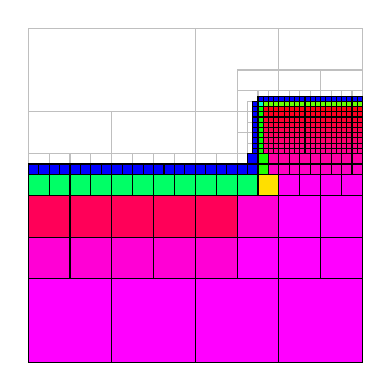
\begin{tikzpicture}[x={(.35\textwidth,0)},y={(0,.35\textwidth)}]
        \def\initiallinewidth{0.4pt}
\definecolor{fillcolor}{rgb}{1.000000,0.000000,1.000000}
\fill[fillcolor] (0.000000,0.000000) rectangle (0.250000,0.250000);
\definecolor{fillcolor}{rgb}{1.000000,0.000000,1.000000}
\fill[fillcolor] (0.250000,0.000000) rectangle (0.500000,0.250000);
\definecolor{fillcolor}{rgb}{1.000000,0.000000,0.834700}
\fill[fillcolor] (0.000000,0.250000) rectangle (0.125000,0.375000);
\definecolor{fillcolor}{rgb}{1.000000,0.000000,0.834700}
\fill[fillcolor] (0.125000,0.250000) rectangle (0.250000,0.375000);
\definecolor{fillcolor}{rgb}{1.000000,0.000000,0.343700}
\fill[fillcolor] (0.000000,0.375000) rectangle (0.125000,0.500000);
\definecolor{fillcolor}{rgb}{1.000000,0.000000,0.343700}
\fill[fillcolor] (0.125000,0.375000) rectangle (0.250000,0.500000);
\definecolor{fillcolor}{rgb}{1.000000,0.000000,0.834700}
\fill[fillcolor] (0.250000,0.250000) rectangle (0.375000,0.375000);
\definecolor{fillcolor}{rgb}{1.000000,0.000000,0.834700}
\fill[fillcolor] (0.375000,0.250000) rectangle (0.500000,0.375000);
\definecolor{fillcolor}{rgb}{1.000000,0.000000,0.343700}
\fill[fillcolor] (0.250000,0.375000) rectangle (0.375000,0.500000);
\definecolor{fillcolor}{rgb}{1.000000,0.000000,0.343700}
\fill[fillcolor] (0.375000,0.375000) rectangle (0.500000,0.500000);
\definecolor{fillcolor}{rgb}{1.000000,0.000000,1.000000}
\fill[fillcolor] (0.500000,0.000000) rectangle (0.750000,0.250000);
\definecolor{fillcolor}{rgb}{1.000000,0.000000,1.000000}
\fill[fillcolor] (0.750000,0.000000) rectangle (1.000000,0.250000);
\definecolor{fillcolor}{rgb}{1.000000,0.000000,0.834700}
\fill[fillcolor] (0.500000,0.250000) rectangle (0.625000,0.375000);
\definecolor{fillcolor}{rgb}{1.000000,0.000000,1.000000}
\fill[fillcolor] (0.625000,0.250000) rectangle (0.750000,0.375000);
\definecolor{fillcolor}{rgb}{1.000000,0.000000,0.343700}
\fill[fillcolor] (0.500000,0.375000) rectangle (0.625000,0.500000);
\definecolor{fillcolor}{rgb}{1.000000,0.000000,0.834700}
\fill[fillcolor] (0.625000,0.375000) rectangle (0.750000,0.500000);
\definecolor{fillcolor}{rgb}{1.000000,0.000000,1.000000}
\fill[fillcolor] (0.750000,0.250000) rectangle (0.875000,0.375000);
\definecolor{fillcolor}{rgb}{1.000000,0.000000,1.000000}
\fill[fillcolor] (0.875000,0.250000) rectangle (1.000000,0.375000);
\definecolor{fillcolor}{rgb}{1.000000,0.000000,1.000000}
\fill[fillcolor] (0.750000,0.375000) rectangle (0.875000,0.500000);
\definecolor{fillcolor}{rgb}{1.000000,0.000000,1.000000}
\fill[fillcolor] (0.875000,0.375000) rectangle (1.000000,0.500000);
\definecolor{fillcolor}{rgb}{0.000000,1.000000,0.400012}
\fill[fillcolor] (0.000000,0.500000) rectangle (0.062500,0.562500);
\definecolor{fillcolor}{rgb}{0.000000,1.000000,0.400012}
\fill[fillcolor] (0.062500,0.500000) rectangle (0.125000,0.562500);
\definecolor{fillcolor}{rgb}{0.000000,0.000000,1.000000}
\fill[fillcolor] (0.000000,0.562500) rectangle (0.031250,0.593750);
\definecolor{fillcolor}{rgb}{0.000000,0.000000,1.000000}
\fill[fillcolor] (0.031250,0.562500) rectangle (0.062500,0.593750);
\definecolor{fillcolor}{rgb}{0.000000,0.000000,1.000000}
\fill[fillcolor] (0.062500,0.562500) rectangle (0.093750,0.593750);
\definecolor{fillcolor}{rgb}{0.000000,0.000000,1.000000}
\fill[fillcolor] (0.093750,0.562500) rectangle (0.125000,0.593750);
\definecolor{fillcolor}{rgb}{0.000000,1.000000,0.400012}
\fill[fillcolor] (0.125000,0.500000) rectangle (0.187500,0.562500);
\definecolor{fillcolor}{rgb}{0.000000,1.000000,0.400012}
\fill[fillcolor] (0.187500,0.500000) rectangle (0.250000,0.562500);
\definecolor{fillcolor}{rgb}{0.000000,0.000000,1.000000}
\fill[fillcolor] (0.125000,0.562500) rectangle (0.156250,0.593750);
\definecolor{fillcolor}{rgb}{0.000000,0.000000,1.000000}
\fill[fillcolor] (0.156250,0.562500) rectangle (0.187500,0.593750);
\definecolor{fillcolor}{rgb}{0.000000,0.000000,1.000000}
\fill[fillcolor] (0.187500,0.562500) rectangle (0.218750,0.593750);
\definecolor{fillcolor}{rgb}{0.000000,0.000000,1.000000}
\fill[fillcolor] (0.218750,0.562500) rectangle (0.250000,0.593750);
\definecolor{fillcolor}{rgb}{0.000000,1.000000,0.400012}
\fill[fillcolor] (0.250000,0.500000) rectangle (0.312500,0.562500);
\definecolor{fillcolor}{rgb}{0.000000,1.000000,0.400012}
\fill[fillcolor] (0.312500,0.500000) rectangle (0.375000,0.562500);
\definecolor{fillcolor}{rgb}{0.000000,0.000000,1.000000}
\fill[fillcolor] (0.250000,0.562500) rectangle (0.281250,0.593750);
\definecolor{fillcolor}{rgb}{0.000000,0.000000,1.000000}
\fill[fillcolor] (0.281250,0.562500) rectangle (0.312500,0.593750);
\definecolor{fillcolor}{rgb}{0.000000,0.000000,1.000000}
\fill[fillcolor] (0.312500,0.562500) rectangle (0.343750,0.593750);
\definecolor{fillcolor}{rgb}{0.000000,0.000000,1.000000}
\fill[fillcolor] (0.343750,0.562500) rectangle (0.375000,0.593750);
\definecolor{fillcolor}{rgb}{0.000000,1.000000,0.400012}
\fill[fillcolor] (0.375000,0.500000) rectangle (0.437500,0.562500);
\definecolor{fillcolor}{rgb}{0.000000,1.000000,0.400012}
\fill[fillcolor] (0.437500,0.500000) rectangle (0.500000,0.562500);
\definecolor{fillcolor}{rgb}{0.000000,0.000000,1.000000}
\fill[fillcolor] (0.375000,0.562500) rectangle (0.406250,0.593750);
\definecolor{fillcolor}{rgb}{0.000000,0.000000,1.000000}
\fill[fillcolor] (0.406250,0.562500) rectangle (0.437500,0.593750);
\definecolor{fillcolor}{rgb}{0.000000,0.000000,1.000000}
\fill[fillcolor] (0.437500,0.562500) rectangle (0.468750,0.593750);
\definecolor{fillcolor}{rgb}{0.000000,0.000000,1.000000}
\fill[fillcolor] (0.468750,0.562500) rectangle (0.500000,0.593750);
\definecolor{fillcolor}{rgb}{0.000000,1.000000,0.400012}
\fill[fillcolor] (0.500000,0.500000) rectangle (0.562500,0.562500);
\definecolor{fillcolor}{rgb}{0.000000,1.000000,0.400012}
\fill[fillcolor] (0.562500,0.500000) rectangle (0.625000,0.562500);
\definecolor{fillcolor}{rgb}{0.000000,0.000000,1.000000}
\fill[fillcolor] (0.500000,0.562500) rectangle (0.531250,0.593750);
\definecolor{fillcolor}{rgb}{0.000000,0.000000,1.000000}
\fill[fillcolor] (0.531250,0.562500) rectangle (0.562500,0.593750);
\definecolor{fillcolor}{rgb}{0.000000,0.000000,1.000000}
\fill[fillcolor] (0.562500,0.562500) rectangle (0.593750,0.593750);
\definecolor{fillcolor}{rgb}{0.000000,0.000000,1.000000}
\fill[fillcolor] (0.593750,0.562500) rectangle (0.625000,0.593750);
\definecolor{fillcolor}{rgb}{0.000000,1.000000,0.400012}
\fill[fillcolor] (0.625000,0.500000) rectangle (0.687500,0.562500);
\definecolor{fillcolor}{rgb}{1.000000,0.873485,0.000000}
\fill[fillcolor] (0.687500,0.500000) rectangle (0.750000,0.562500);
\definecolor{fillcolor}{rgb}{0.000000,0.000000,1.000000}
\fill[fillcolor] (0.625000,0.562500) rectangle (0.656250,0.593750);
\definecolor{fillcolor}{rgb}{0.000000,0.000000,1.000000}
\fill[fillcolor] (0.656250,0.562500) rectangle (0.687500,0.593750);
\definecolor{fillcolor}{rgb}{0.000000,0.000000,1.000000}
\fill[fillcolor] (0.656250,0.593750) rectangle (0.687500,0.625000);
\definecolor{fillcolor}{rgb}{0.141162,1.000000,0.000000}
\fill[fillcolor] (0.687500,0.562500) rectangle (0.718750,0.593750);
\definecolor{fillcolor}{rgb}{1.000000,0.000000,0.773325}
\fill[fillcolor] (0.718750,0.562500) rectangle (0.750000,0.593750);
\definecolor{fillcolor}{rgb}{0.079788,1.000000,0.000000}
\fill[fillcolor] (0.687500,0.593750) rectangle (0.718750,0.625000);
\definecolor{fillcolor}{rgb}{1.000000,0.000000,0.650575}
\fill[fillcolor] (0.718750,0.593750) rectangle (0.750000,0.625000);
\definecolor{fillcolor}{rgb}{0.000000,0.000000,1.000000}
\fill[fillcolor] (0.671875,0.625000) rectangle (0.687500,0.640625);
\definecolor{fillcolor}{rgb}{0.000000,0.000000,1.000000}
\fill[fillcolor] (0.671875,0.640625) rectangle (0.687500,0.656250);
\definecolor{fillcolor}{rgb}{0.000000,0.000000,1.000000}
\fill[fillcolor] (0.671875,0.656250) rectangle (0.687500,0.671875);
\definecolor{fillcolor}{rgb}{0.000000,0.000000,1.000000}
\fill[fillcolor] (0.671875,0.671875) rectangle (0.687500,0.687500);
\definecolor{fillcolor}{rgb}{0.033756,1.000000,0.000000}
\fill[fillcolor] (0.687500,0.625000) rectangle (0.703125,0.640625);
\definecolor{fillcolor}{rgb}{1.000000,0.000000,0.558513}
\fill[fillcolor] (0.703125,0.625000) rectangle (0.718750,0.640625);
\definecolor{fillcolor}{rgb}{0.003069,1.000000,0.000000}
\fill[fillcolor] (0.687500,0.640625) rectangle (0.703125,0.656250);
\definecolor{fillcolor}{rgb}{1.000000,0.000000,0.497137}
\fill[fillcolor] (0.703125,0.640625) rectangle (0.718750,0.656250);
\definecolor{fillcolor}{rgb}{1.000000,0.000000,0.558513}
\fill[fillcolor] (0.718750,0.625000) rectangle (0.734375,0.640625);
\definecolor{fillcolor}{rgb}{1.000000,0.000000,0.558513}
\fill[fillcolor] (0.734375,0.625000) rectangle (0.750000,0.640625);
\definecolor{fillcolor}{rgb}{1.000000,0.000000,0.497137}
\fill[fillcolor] (0.718750,0.640625) rectangle (0.734375,0.656250);
\definecolor{fillcolor}{rgb}{1.000000,0.000000,0.497137}
\fill[fillcolor] (0.734375,0.640625) rectangle (0.750000,0.656250);
\definecolor{fillcolor}{rgb}{0.000000,1.000000,0.000034}
\fill[fillcolor] (0.687500,0.656250) rectangle (0.703125,0.671875);
\definecolor{fillcolor}{rgb}{1.000000,0.000000,0.435762}
\fill[fillcolor] (0.703125,0.656250) rectangle (0.718750,0.671875);
\definecolor{fillcolor}{rgb}{0.000000,1.000000,0.000073}
\fill[fillcolor] (0.687500,0.671875) rectangle (0.703125,0.687500);
\definecolor{fillcolor}{rgb}{1.000000,0.000000,0.374388}
\fill[fillcolor] (0.703125,0.671875) rectangle (0.718750,0.687500);
\definecolor{fillcolor}{rgb}{1.000000,0.000000,0.435762}
\fill[fillcolor] (0.718750,0.656250) rectangle (0.734375,0.671875);
\definecolor{fillcolor}{rgb}{1.000000,0.000000,0.435762}
\fill[fillcolor] (0.734375,0.656250) rectangle (0.750000,0.671875);
\definecolor{fillcolor}{rgb}{1.000000,0.000000,0.374388}
\fill[fillcolor] (0.718750,0.671875) rectangle (0.734375,0.687500);
\definecolor{fillcolor}{rgb}{1.000000,0.000000,0.374388}
\fill[fillcolor] (0.734375,0.671875) rectangle (0.750000,0.687500);
\definecolor{fillcolor}{rgb}{0.000000,0.000000,1.000000}
\fill[fillcolor] (0.671875,0.687500) rectangle (0.687500,0.703125);
\definecolor{fillcolor}{rgb}{0.000000,0.000000,1.000000}
\fill[fillcolor] (0.671875,0.703125) rectangle (0.687500,0.718750);
\definecolor{fillcolor}{rgb}{0.000000,0.000000,1.000000}
\fill[fillcolor] (0.671875,0.718750) rectangle (0.687500,0.734375);
\definecolor{fillcolor}{rgb}{0.000000,0.000000,1.000000}
\fill[fillcolor] (0.671875,0.734375) rectangle (0.687500,0.750000);
\definecolor{fillcolor}{rgb}{0.000000,1.000000,0.000111}
\fill[fillcolor] (0.687500,0.687500) rectangle (0.703125,0.703125);
\definecolor{fillcolor}{rgb}{1.000000,0.000000,0.313013}
\fill[fillcolor] (0.703125,0.687500) rectangle (0.718750,0.703125);
\definecolor{fillcolor}{rgb}{0.000000,1.000000,0.000149}
\fill[fillcolor] (0.687500,0.703125) rectangle (0.703125,0.718750);
\definecolor{fillcolor}{rgb}{1.000000,0.000000,0.251637}
\fill[fillcolor] (0.703125,0.703125) rectangle (0.718750,0.718750);
\definecolor{fillcolor}{rgb}{1.000000,0.000000,0.313013}
\fill[fillcolor] (0.718750,0.687500) rectangle (0.734375,0.703125);
\definecolor{fillcolor}{rgb}{1.000000,0.000000,0.313013}
\fill[fillcolor] (0.734375,0.687500) rectangle (0.750000,0.703125);
\definecolor{fillcolor}{rgb}{1.000000,0.000000,0.251637}
\fill[fillcolor] (0.718750,0.703125) rectangle (0.734375,0.718750);
\definecolor{fillcolor}{rgb}{1.000000,0.000000,0.251637}
\fill[fillcolor] (0.734375,0.703125) rectangle (0.750000,0.718750);
\definecolor{fillcolor}{rgb}{0.000000,1.000000,0.000187}
\fill[fillcolor] (0.687500,0.718750) rectangle (0.703125,0.734375);
\definecolor{fillcolor}{rgb}{1.000000,0.000000,0.190262}
\fill[fillcolor] (0.703125,0.718750) rectangle (0.718750,0.734375);
\definecolor{fillcolor}{rgb}{0.000000,1.000000,0.000224}
\fill[fillcolor] (0.687500,0.734375) rectangle (0.703125,0.750000);
\definecolor{fillcolor}{rgb}{1.000000,0.000000,0.128888}
\fill[fillcolor] (0.703125,0.734375) rectangle (0.718750,0.750000);
\definecolor{fillcolor}{rgb}{1.000000,0.000000,0.190262}
\fill[fillcolor] (0.718750,0.718750) rectangle (0.734375,0.734375);
\definecolor{fillcolor}{rgb}{1.000000,0.000000,0.190262}
\fill[fillcolor] (0.734375,0.718750) rectangle (0.750000,0.734375);
\definecolor{fillcolor}{rgb}{1.000000,0.000000,0.128888}
\fill[fillcolor] (0.718750,0.734375) rectangle (0.734375,0.750000);
\definecolor{fillcolor}{rgb}{1.000000,0.000000,0.128888}
\fill[fillcolor] (0.734375,0.734375) rectangle (0.750000,0.750000);
\definecolor{fillcolor}{rgb}{1.000000,0.000000,0.957450}
\fill[fillcolor] (0.750000,0.500000) rectangle (0.812500,0.562500);
\definecolor{fillcolor}{rgb}{1.000000,0.000000,0.957450}
\fill[fillcolor] (0.812500,0.500000) rectangle (0.875000,0.562500);
\definecolor{fillcolor}{rgb}{1.000000,0.000000,0.773325}
\fill[fillcolor] (0.750000,0.562500) rectangle (0.781250,0.593750);
\definecolor{fillcolor}{rgb}{1.000000,0.000000,0.773325}
\fill[fillcolor] (0.781250,0.562500) rectangle (0.812500,0.593750);
\definecolor{fillcolor}{rgb}{1.000000,0.000000,0.650575}
\fill[fillcolor] (0.750000,0.593750) rectangle (0.781250,0.625000);
\definecolor{fillcolor}{rgb}{1.000000,0.000000,0.650575}
\fill[fillcolor] (0.781250,0.593750) rectangle (0.812500,0.625000);
\definecolor{fillcolor}{rgb}{1.000000,0.000000,0.773325}
\fill[fillcolor] (0.812500,0.562500) rectangle (0.843750,0.593750);
\definecolor{fillcolor}{rgb}{1.000000,0.000000,0.773325}
\fill[fillcolor] (0.843750,0.562500) rectangle (0.875000,0.593750);
\definecolor{fillcolor}{rgb}{1.000000,0.000000,0.650575}
\fill[fillcolor] (0.812500,0.593750) rectangle (0.843750,0.625000);
\definecolor{fillcolor}{rgb}{1.000000,0.000000,0.650575}
\fill[fillcolor] (0.843750,0.593750) rectangle (0.875000,0.625000);
\definecolor{fillcolor}{rgb}{1.000000,0.000000,0.957450}
\fill[fillcolor] (0.875000,0.500000) rectangle (0.937500,0.562500);
\definecolor{fillcolor}{rgb}{1.000000,0.000000,0.957450}
\fill[fillcolor] (0.937500,0.500000) rectangle (1.000000,0.562500);
\definecolor{fillcolor}{rgb}{1.000000,0.000000,0.773325}
\fill[fillcolor] (0.875000,0.562500) rectangle (0.906250,0.593750);
\definecolor{fillcolor}{rgb}{1.000000,0.000000,0.773325}
\fill[fillcolor] (0.906250,0.562500) rectangle (0.937500,0.593750);
\definecolor{fillcolor}{rgb}{1.000000,0.000000,0.650575}
\fill[fillcolor] (0.875000,0.593750) rectangle (0.906250,0.625000);
\definecolor{fillcolor}{rgb}{1.000000,0.000000,0.650575}
\fill[fillcolor] (0.906250,0.593750) rectangle (0.937500,0.625000);
\definecolor{fillcolor}{rgb}{1.000000,0.000000,0.773325}
\fill[fillcolor] (0.937500,0.562500) rectangle (0.968750,0.593750);
\definecolor{fillcolor}{rgb}{1.000000,0.000000,0.773325}
\fill[fillcolor] (0.968750,0.562500) rectangle (1.000000,0.593750);
\definecolor{fillcolor}{rgb}{1.000000,0.000000,0.650575}
\fill[fillcolor] (0.937500,0.593750) rectangle (0.968750,0.625000);
\definecolor{fillcolor}{rgb}{1.000000,0.000000,0.650575}
\fill[fillcolor] (0.968750,0.593750) rectangle (1.000000,0.625000);
\definecolor{fillcolor}{rgb}{1.000000,0.000000,0.558513}
\fill[fillcolor] (0.750000,0.625000) rectangle (0.765625,0.640625);
\definecolor{fillcolor}{rgb}{1.000000,0.000000,0.558513}
\fill[fillcolor] (0.765625,0.625000) rectangle (0.781250,0.640625);
\definecolor{fillcolor}{rgb}{1.000000,0.000000,0.497137}
\fill[fillcolor] (0.750000,0.640625) rectangle (0.765625,0.656250);
\definecolor{fillcolor}{rgb}{1.000000,0.000000,0.497137}
\fill[fillcolor] (0.765625,0.640625) rectangle (0.781250,0.656250);
\definecolor{fillcolor}{rgb}{1.000000,0.000000,0.558513}
\fill[fillcolor] (0.781250,0.625000) rectangle (0.796875,0.640625);
\definecolor{fillcolor}{rgb}{1.000000,0.000000,0.558513}
\fill[fillcolor] (0.796875,0.625000) rectangle (0.812500,0.640625);
\definecolor{fillcolor}{rgb}{1.000000,0.000000,0.497137}
\fill[fillcolor] (0.781250,0.640625) rectangle (0.796875,0.656250);
\definecolor{fillcolor}{rgb}{1.000000,0.000000,0.497137}
\fill[fillcolor] (0.796875,0.640625) rectangle (0.812500,0.656250);
\definecolor{fillcolor}{rgb}{1.000000,0.000000,0.435762}
\fill[fillcolor] (0.750000,0.656250) rectangle (0.765625,0.671875);
\definecolor{fillcolor}{rgb}{1.000000,0.000000,0.435762}
\fill[fillcolor] (0.765625,0.656250) rectangle (0.781250,0.671875);
\definecolor{fillcolor}{rgb}{1.000000,0.000000,0.374388}
\fill[fillcolor] (0.750000,0.671875) rectangle (0.765625,0.687500);
\definecolor{fillcolor}{rgb}{1.000000,0.000000,0.374388}
\fill[fillcolor] (0.765625,0.671875) rectangle (0.781250,0.687500);
\definecolor{fillcolor}{rgb}{1.000000,0.000000,0.435762}
\fill[fillcolor] (0.781250,0.656250) rectangle (0.796875,0.671875);
\definecolor{fillcolor}{rgb}{1.000000,0.000000,0.435762}
\fill[fillcolor] (0.796875,0.656250) rectangle (0.812500,0.671875);
\definecolor{fillcolor}{rgb}{1.000000,0.000000,0.374388}
\fill[fillcolor] (0.781250,0.671875) rectangle (0.796875,0.687500);
\definecolor{fillcolor}{rgb}{1.000000,0.000000,0.374388}
\fill[fillcolor] (0.796875,0.671875) rectangle (0.812500,0.687500);
\definecolor{fillcolor}{rgb}{1.000000,0.000000,0.558513}
\fill[fillcolor] (0.812500,0.625000) rectangle (0.828125,0.640625);
\definecolor{fillcolor}{rgb}{1.000000,0.000000,0.558513}
\fill[fillcolor] (0.828125,0.625000) rectangle (0.843750,0.640625);
\definecolor{fillcolor}{rgb}{1.000000,0.000000,0.497137}
\fill[fillcolor] (0.812500,0.640625) rectangle (0.828125,0.656250);
\definecolor{fillcolor}{rgb}{1.000000,0.000000,0.497137}
\fill[fillcolor] (0.828125,0.640625) rectangle (0.843750,0.656250);
\definecolor{fillcolor}{rgb}{1.000000,0.000000,0.558513}
\fill[fillcolor] (0.843750,0.625000) rectangle (0.859375,0.640625);
\definecolor{fillcolor}{rgb}{1.000000,0.000000,0.558513}
\fill[fillcolor] (0.859375,0.625000) rectangle (0.875000,0.640625);
\definecolor{fillcolor}{rgb}{1.000000,0.000000,0.497137}
\fill[fillcolor] (0.843750,0.640625) rectangle (0.859375,0.656250);
\definecolor{fillcolor}{rgb}{1.000000,0.000000,0.497137}
\fill[fillcolor] (0.859375,0.640625) rectangle (0.875000,0.656250);
\definecolor{fillcolor}{rgb}{1.000000,0.000000,0.435762}
\fill[fillcolor] (0.812500,0.656250) rectangle (0.828125,0.671875);
\definecolor{fillcolor}{rgb}{1.000000,0.000000,0.435762}
\fill[fillcolor] (0.828125,0.656250) rectangle (0.843750,0.671875);
\definecolor{fillcolor}{rgb}{1.000000,0.000000,0.374388}
\fill[fillcolor] (0.812500,0.671875) rectangle (0.828125,0.687500);
\definecolor{fillcolor}{rgb}{1.000000,0.000000,0.374388}
\fill[fillcolor] (0.828125,0.671875) rectangle (0.843750,0.687500);
\definecolor{fillcolor}{rgb}{1.000000,0.000000,0.435762}
\fill[fillcolor] (0.843750,0.656250) rectangle (0.859375,0.671875);
\definecolor{fillcolor}{rgb}{1.000000,0.000000,0.435762}
\fill[fillcolor] (0.859375,0.656250) rectangle (0.875000,0.671875);
\definecolor{fillcolor}{rgb}{1.000000,0.000000,0.374388}
\fill[fillcolor] (0.843750,0.671875) rectangle (0.859375,0.687500);
\definecolor{fillcolor}{rgb}{1.000000,0.000000,0.374388}
\fill[fillcolor] (0.859375,0.671875) rectangle (0.875000,0.687500);
\definecolor{fillcolor}{rgb}{1.000000,0.000000,0.313013}
\fill[fillcolor] (0.750000,0.687500) rectangle (0.765625,0.703125);
\definecolor{fillcolor}{rgb}{1.000000,0.000000,0.313013}
\fill[fillcolor] (0.765625,0.687500) rectangle (0.781250,0.703125);
\definecolor{fillcolor}{rgb}{1.000000,0.000000,0.251637}
\fill[fillcolor] (0.750000,0.703125) rectangle (0.765625,0.718750);
\definecolor{fillcolor}{rgb}{1.000000,0.000000,0.251637}
\fill[fillcolor] (0.765625,0.703125) rectangle (0.781250,0.718750);
\definecolor{fillcolor}{rgb}{1.000000,0.000000,0.313013}
\fill[fillcolor] (0.781250,0.687500) rectangle (0.796875,0.703125);
\definecolor{fillcolor}{rgb}{1.000000,0.000000,0.313013}
\fill[fillcolor] (0.796875,0.687500) rectangle (0.812500,0.703125);
\definecolor{fillcolor}{rgb}{1.000000,0.000000,0.251637}
\fill[fillcolor] (0.781250,0.703125) rectangle (0.796875,0.718750);
\definecolor{fillcolor}{rgb}{1.000000,0.000000,0.251637}
\fill[fillcolor] (0.796875,0.703125) rectangle (0.812500,0.718750);
\definecolor{fillcolor}{rgb}{1.000000,0.000000,0.190262}
\fill[fillcolor] (0.750000,0.718750) rectangle (0.765625,0.734375);
\definecolor{fillcolor}{rgb}{1.000000,0.000000,0.190262}
\fill[fillcolor] (0.765625,0.718750) rectangle (0.781250,0.734375);
\definecolor{fillcolor}{rgb}{1.000000,0.000000,0.128888}
\fill[fillcolor] (0.750000,0.734375) rectangle (0.765625,0.750000);
\definecolor{fillcolor}{rgb}{1.000000,0.000000,0.128888}
\fill[fillcolor] (0.765625,0.734375) rectangle (0.781250,0.750000);
\definecolor{fillcolor}{rgb}{1.000000,0.000000,0.190262}
\fill[fillcolor] (0.781250,0.718750) rectangle (0.796875,0.734375);
\definecolor{fillcolor}{rgb}{1.000000,0.000000,0.190262}
\fill[fillcolor] (0.796875,0.718750) rectangle (0.812500,0.734375);
\definecolor{fillcolor}{rgb}{1.000000,0.000000,0.128888}
\fill[fillcolor] (0.781250,0.734375) rectangle (0.796875,0.750000);
\definecolor{fillcolor}{rgb}{1.000000,0.000000,0.128888}
\fill[fillcolor] (0.796875,0.734375) rectangle (0.812500,0.750000);
\definecolor{fillcolor}{rgb}{1.000000,0.000000,0.313013}
\fill[fillcolor] (0.812500,0.687500) rectangle (0.828125,0.703125);
\definecolor{fillcolor}{rgb}{1.000000,0.000000,0.313013}
\fill[fillcolor] (0.828125,0.687500) rectangle (0.843750,0.703125);
\definecolor{fillcolor}{rgb}{1.000000,0.000000,0.251637}
\fill[fillcolor] (0.812500,0.703125) rectangle (0.828125,0.718750);
\definecolor{fillcolor}{rgb}{1.000000,0.000000,0.251637}
\fill[fillcolor] (0.828125,0.703125) rectangle (0.843750,0.718750);
\definecolor{fillcolor}{rgb}{1.000000,0.000000,0.313013}
\fill[fillcolor] (0.843750,0.687500) rectangle (0.859375,0.703125);
\definecolor{fillcolor}{rgb}{1.000000,0.000000,0.313013}
\fill[fillcolor] (0.859375,0.687500) rectangle (0.875000,0.703125);
\definecolor{fillcolor}{rgb}{1.000000,0.000000,0.251637}
\fill[fillcolor] (0.843750,0.703125) rectangle (0.859375,0.718750);
\definecolor{fillcolor}{rgb}{1.000000,0.000000,0.251637}
\fill[fillcolor] (0.859375,0.703125) rectangle (0.875000,0.718750);
\definecolor{fillcolor}{rgb}{1.000000,0.000000,0.190262}
\fill[fillcolor] (0.812500,0.718750) rectangle (0.828125,0.734375);
\definecolor{fillcolor}{rgb}{1.000000,0.000000,0.190262}
\fill[fillcolor] (0.828125,0.718750) rectangle (0.843750,0.734375);
\definecolor{fillcolor}{rgb}{1.000000,0.000000,0.128888}
\fill[fillcolor] (0.812500,0.734375) rectangle (0.828125,0.750000);
\definecolor{fillcolor}{rgb}{1.000000,0.000000,0.128888}
\fill[fillcolor] (0.828125,0.734375) rectangle (0.843750,0.750000);
\definecolor{fillcolor}{rgb}{1.000000,0.000000,0.190262}
\fill[fillcolor] (0.843750,0.718750) rectangle (0.859375,0.734375);
\definecolor{fillcolor}{rgb}{1.000000,0.000000,0.190262}
\fill[fillcolor] (0.859375,0.718750) rectangle (0.875000,0.734375);
\definecolor{fillcolor}{rgb}{1.000000,0.000000,0.128888}
\fill[fillcolor] (0.843750,0.734375) rectangle (0.859375,0.750000);
\definecolor{fillcolor}{rgb}{1.000000,0.000000,0.128888}
\fill[fillcolor] (0.859375,0.734375) rectangle (0.875000,0.750000);
\definecolor{fillcolor}{rgb}{1.000000,0.000000,0.558513}
\fill[fillcolor] (0.875000,0.625000) rectangle (0.890625,0.640625);
\definecolor{fillcolor}{rgb}{1.000000,0.000000,0.558513}
\fill[fillcolor] (0.890625,0.625000) rectangle (0.906250,0.640625);
\definecolor{fillcolor}{rgb}{1.000000,0.000000,0.497137}
\fill[fillcolor] (0.875000,0.640625) rectangle (0.890625,0.656250);
\definecolor{fillcolor}{rgb}{1.000000,0.000000,0.497137}
\fill[fillcolor] (0.890625,0.640625) rectangle (0.906250,0.656250);
\definecolor{fillcolor}{rgb}{1.000000,0.000000,0.558513}
\fill[fillcolor] (0.906250,0.625000) rectangle (0.921875,0.640625);
\definecolor{fillcolor}{rgb}{1.000000,0.000000,0.558513}
\fill[fillcolor] (0.921875,0.625000) rectangle (0.937500,0.640625);
\definecolor{fillcolor}{rgb}{1.000000,0.000000,0.497137}
\fill[fillcolor] (0.906250,0.640625) rectangle (0.921875,0.656250);
\definecolor{fillcolor}{rgb}{1.000000,0.000000,0.497137}
\fill[fillcolor] (0.921875,0.640625) rectangle (0.937500,0.656250);
\definecolor{fillcolor}{rgb}{1.000000,0.000000,0.435762}
\fill[fillcolor] (0.875000,0.656250) rectangle (0.890625,0.671875);
\definecolor{fillcolor}{rgb}{1.000000,0.000000,0.435762}
\fill[fillcolor] (0.890625,0.656250) rectangle (0.906250,0.671875);
\definecolor{fillcolor}{rgb}{1.000000,0.000000,0.374388}
\fill[fillcolor] (0.875000,0.671875) rectangle (0.890625,0.687500);
\definecolor{fillcolor}{rgb}{1.000000,0.000000,0.374388}
\fill[fillcolor] (0.890625,0.671875) rectangle (0.906250,0.687500);
\definecolor{fillcolor}{rgb}{1.000000,0.000000,0.435762}
\fill[fillcolor] (0.906250,0.656250) rectangle (0.921875,0.671875);
\definecolor{fillcolor}{rgb}{1.000000,0.000000,0.435762}
\fill[fillcolor] (0.921875,0.656250) rectangle (0.937500,0.671875);
\definecolor{fillcolor}{rgb}{1.000000,0.000000,0.374388}
\fill[fillcolor] (0.906250,0.671875) rectangle (0.921875,0.687500);
\definecolor{fillcolor}{rgb}{1.000000,0.000000,0.374388}
\fill[fillcolor] (0.921875,0.671875) rectangle (0.937500,0.687500);
\definecolor{fillcolor}{rgb}{1.000000,0.000000,0.558513}
\fill[fillcolor] (0.937500,0.625000) rectangle (0.953125,0.640625);
\definecolor{fillcolor}{rgb}{1.000000,0.000000,0.558513}
\fill[fillcolor] (0.953125,0.625000) rectangle (0.968750,0.640625);
\definecolor{fillcolor}{rgb}{1.000000,0.000000,0.497137}
\fill[fillcolor] (0.937500,0.640625) rectangle (0.953125,0.656250);
\definecolor{fillcolor}{rgb}{1.000000,0.000000,0.497137}
\fill[fillcolor] (0.953125,0.640625) rectangle (0.968750,0.656250);
\definecolor{fillcolor}{rgb}{1.000000,0.000000,0.558513}
\fill[fillcolor] (0.968750,0.625000) rectangle (0.984375,0.640625);
\definecolor{fillcolor}{rgb}{1.000000,0.000000,0.558513}
\fill[fillcolor] (0.984375,0.625000) rectangle (1.000000,0.640625);
\definecolor{fillcolor}{rgb}{1.000000,0.000000,0.497137}
\fill[fillcolor] (0.968750,0.640625) rectangle (0.984375,0.656250);
\definecolor{fillcolor}{rgb}{1.000000,0.000000,0.497137}
\fill[fillcolor] (0.984375,0.640625) rectangle (1.000000,0.656250);
\definecolor{fillcolor}{rgb}{1.000000,0.000000,0.435762}
\fill[fillcolor] (0.937500,0.656250) rectangle (0.953125,0.671875);
\definecolor{fillcolor}{rgb}{1.000000,0.000000,0.435762}
\fill[fillcolor] (0.953125,0.656250) rectangle (0.968750,0.671875);
\definecolor{fillcolor}{rgb}{1.000000,0.000000,0.374388}
\fill[fillcolor] (0.937500,0.671875) rectangle (0.953125,0.687500);
\definecolor{fillcolor}{rgb}{1.000000,0.000000,0.374388}
\fill[fillcolor] (0.953125,0.671875) rectangle (0.968750,0.687500);
\definecolor{fillcolor}{rgb}{1.000000,0.000000,0.435762}
\fill[fillcolor] (0.968750,0.656250) rectangle (0.984375,0.671875);
\definecolor{fillcolor}{rgb}{1.000000,0.000000,0.435762}
\fill[fillcolor] (0.984375,0.656250) rectangle (1.000000,0.671875);
\definecolor{fillcolor}{rgb}{1.000000,0.000000,0.374388}
\fill[fillcolor] (0.968750,0.671875) rectangle (0.984375,0.687500);
\definecolor{fillcolor}{rgb}{1.000000,0.000000,0.374388}
\fill[fillcolor] (0.984375,0.671875) rectangle (1.000000,0.687500);
\definecolor{fillcolor}{rgb}{1.000000,0.000000,0.313013}
\fill[fillcolor] (0.875000,0.687500) rectangle (0.890625,0.703125);
\definecolor{fillcolor}{rgb}{1.000000,0.000000,0.313013}
\fill[fillcolor] (0.890625,0.687500) rectangle (0.906250,0.703125);
\definecolor{fillcolor}{rgb}{1.000000,0.000000,0.251637}
\fill[fillcolor] (0.875000,0.703125) rectangle (0.890625,0.718750);
\definecolor{fillcolor}{rgb}{1.000000,0.000000,0.251637}
\fill[fillcolor] (0.890625,0.703125) rectangle (0.906250,0.718750);
\definecolor{fillcolor}{rgb}{1.000000,0.000000,0.313013}
\fill[fillcolor] (0.906250,0.687500) rectangle (0.921875,0.703125);
\definecolor{fillcolor}{rgb}{1.000000,0.000000,0.313013}
\fill[fillcolor] (0.921875,0.687500) rectangle (0.937500,0.703125);
\definecolor{fillcolor}{rgb}{1.000000,0.000000,0.251637}
\fill[fillcolor] (0.906250,0.703125) rectangle (0.921875,0.718750);
\definecolor{fillcolor}{rgb}{1.000000,0.000000,0.251637}
\fill[fillcolor] (0.921875,0.703125) rectangle (0.937500,0.718750);
\definecolor{fillcolor}{rgb}{1.000000,0.000000,0.190262}
\fill[fillcolor] (0.875000,0.718750) rectangle (0.890625,0.734375);
\definecolor{fillcolor}{rgb}{1.000000,0.000000,0.190262}
\fill[fillcolor] (0.890625,0.718750) rectangle (0.906250,0.734375);
\definecolor{fillcolor}{rgb}{1.000000,0.000000,0.128888}
\fill[fillcolor] (0.875000,0.734375) rectangle (0.890625,0.750000);
\definecolor{fillcolor}{rgb}{1.000000,0.000000,0.128888}
\fill[fillcolor] (0.890625,0.734375) rectangle (0.906250,0.750000);
\definecolor{fillcolor}{rgb}{1.000000,0.000000,0.190262}
\fill[fillcolor] (0.906250,0.718750) rectangle (0.921875,0.734375);
\definecolor{fillcolor}{rgb}{1.000000,0.000000,0.190262}
\fill[fillcolor] (0.921875,0.718750) rectangle (0.937500,0.734375);
\definecolor{fillcolor}{rgb}{1.000000,0.000000,0.128888}
\fill[fillcolor] (0.906250,0.734375) rectangle (0.921875,0.750000);
\definecolor{fillcolor}{rgb}{1.000000,0.000000,0.128888}
\fill[fillcolor] (0.921875,0.734375) rectangle (0.937500,0.750000);
\definecolor{fillcolor}{rgb}{1.000000,0.000000,0.313013}
\fill[fillcolor] (0.937500,0.687500) rectangle (0.953125,0.703125);
\definecolor{fillcolor}{rgb}{1.000000,0.000000,0.313013}
\fill[fillcolor] (0.953125,0.687500) rectangle (0.968750,0.703125);
\definecolor{fillcolor}{rgb}{1.000000,0.000000,0.251637}
\fill[fillcolor] (0.937500,0.703125) rectangle (0.953125,0.718750);
\definecolor{fillcolor}{rgb}{1.000000,0.000000,0.251637}
\fill[fillcolor] (0.953125,0.703125) rectangle (0.968750,0.718750);
\definecolor{fillcolor}{rgb}{1.000000,0.000000,0.313013}
\fill[fillcolor] (0.968750,0.687500) rectangle (0.984375,0.703125);
\definecolor{fillcolor}{rgb}{1.000000,0.000000,0.313013}
\fill[fillcolor] (0.984375,0.687500) rectangle (1.000000,0.703125);
\definecolor{fillcolor}{rgb}{1.000000,0.000000,0.251637}
\fill[fillcolor] (0.968750,0.703125) rectangle (0.984375,0.718750);
\definecolor{fillcolor}{rgb}{1.000000,0.000000,0.251637}
\fill[fillcolor] (0.984375,0.703125) rectangle (1.000000,0.718750);
\definecolor{fillcolor}{rgb}{1.000000,0.000000,0.190262}
\fill[fillcolor] (0.937500,0.718750) rectangle (0.953125,0.734375);
\definecolor{fillcolor}{rgb}{1.000000,0.000000,0.190262}
\fill[fillcolor] (0.953125,0.718750) rectangle (0.968750,0.734375);
\definecolor{fillcolor}{rgb}{1.000000,0.000000,0.128888}
\fill[fillcolor] (0.937500,0.734375) rectangle (0.953125,0.750000);
\definecolor{fillcolor}{rgb}{1.000000,0.000000,0.128888}
\fill[fillcolor] (0.953125,0.734375) rectangle (0.968750,0.750000);
\definecolor{fillcolor}{rgb}{1.000000,0.000000,0.190262}
\fill[fillcolor] (0.968750,0.718750) rectangle (0.984375,0.734375);
\definecolor{fillcolor}{rgb}{1.000000,0.000000,0.190262}
\fill[fillcolor] (0.984375,0.718750) rectangle (1.000000,0.734375);
\definecolor{fillcolor}{rgb}{1.000000,0.000000,0.128888}
\fill[fillcolor] (0.968750,0.734375) rectangle (0.984375,0.750000);
\definecolor{fillcolor}{rgb}{1.000000,0.000000,0.128888}
\fill[fillcolor] (0.984375,0.734375) rectangle (1.000000,0.750000);
\definecolor{fillcolor}{rgb}{0.000000,0.000000,1.000000}
\fill[fillcolor] (0.671875,0.750000) rectangle (0.687500,0.765625);
\definecolor{fillcolor}{rgb}{0.000000,0.000000,1.000000}
\fill[fillcolor] (0.671875,0.765625) rectangle (0.687500,0.781250);
\definecolor{fillcolor}{rgb}{0.000000,1.000000,0.000262}
\fill[fillcolor] (0.687500,0.750000) rectangle (0.703125,0.765625);
\definecolor{fillcolor}{rgb}{1.000000,0.000000,0.067512}
\fill[fillcolor] (0.703125,0.750000) rectangle (0.718750,0.765625);
\definecolor{fillcolor}{rgb}{0.000000,1.000000,0.800180}
\fill[fillcolor] (0.687500,0.765625) rectangle (0.703125,0.781250);
\definecolor{fillcolor}{rgb}{0.403683,1.000000,0.000000}
\fill[fillcolor] (0.703125,0.765625) rectangle (0.718750,0.781250);
\definecolor{fillcolor}{rgb}{1.000000,0.000000,0.067512}
\fill[fillcolor] (0.718750,0.750000) rectangle (0.734375,0.765625);
\definecolor{fillcolor}{rgb}{1.000000,0.000000,0.067512}
\fill[fillcolor] (0.734375,0.750000) rectangle (0.750000,0.765625);
\definecolor{fillcolor}{rgb}{0.403683,1.000000,0.000000}
\fill[fillcolor] (0.718750,0.765625) rectangle (0.734375,0.781250);
\definecolor{fillcolor}{rgb}{0.403683,1.000000,0.000000}
\fill[fillcolor] (0.734375,0.765625) rectangle (0.750000,0.781250);
\definecolor{fillcolor}{rgb}{0.000000,0.000000,1.000000}
\fill[fillcolor] (0.687500,0.781250) rectangle (0.703125,0.796875);
\definecolor{fillcolor}{rgb}{0.000000,0.000000,1.000000}
\fill[fillcolor] (0.703125,0.781250) rectangle (0.718750,0.796875);
\definecolor{fillcolor}{rgb}{0.000000,0.000000,1.000000}
\fill[fillcolor] (0.718750,0.781250) rectangle (0.734375,0.796875);
\definecolor{fillcolor}{rgb}{0.000000,0.000000,1.000000}
\fill[fillcolor] (0.734375,0.781250) rectangle (0.750000,0.796875);
\definecolor{fillcolor}{rgb}{1.000000,0.000000,0.067512}
\fill[fillcolor] (0.750000,0.750000) rectangle (0.765625,0.765625);
\definecolor{fillcolor}{rgb}{1.000000,0.000000,0.067512}
\fill[fillcolor] (0.765625,0.750000) rectangle (0.781250,0.765625);
\definecolor{fillcolor}{rgb}{0.403683,1.000000,0.000000}
\fill[fillcolor] (0.750000,0.765625) rectangle (0.765625,0.781250);
\definecolor{fillcolor}{rgb}{0.403683,1.000000,0.000000}
\fill[fillcolor] (0.765625,0.765625) rectangle (0.781250,0.781250);
\definecolor{fillcolor}{rgb}{1.000000,0.000000,0.067512}
\fill[fillcolor] (0.781250,0.750000) rectangle (0.796875,0.765625);
\definecolor{fillcolor}{rgb}{1.000000,0.000000,0.067512}
\fill[fillcolor] (0.796875,0.750000) rectangle (0.812500,0.765625);
\definecolor{fillcolor}{rgb}{0.403683,1.000000,0.000000}
\fill[fillcolor] (0.781250,0.765625) rectangle (0.796875,0.781250);
\definecolor{fillcolor}{rgb}{0.403683,1.000000,0.000000}
\fill[fillcolor] (0.796875,0.765625) rectangle (0.812500,0.781250);
\definecolor{fillcolor}{rgb}{0.000000,0.000000,1.000000}
\fill[fillcolor] (0.750000,0.781250) rectangle (0.765625,0.796875);
\definecolor{fillcolor}{rgb}{0.000000,0.000000,1.000000}
\fill[fillcolor] (0.765625,0.781250) rectangle (0.781250,0.796875);
\definecolor{fillcolor}{rgb}{0.000000,0.000000,1.000000}
\fill[fillcolor] (0.781250,0.781250) rectangle (0.796875,0.796875);
\definecolor{fillcolor}{rgb}{0.000000,0.000000,1.000000}
\fill[fillcolor] (0.796875,0.781250) rectangle (0.812500,0.796875);
\definecolor{fillcolor}{rgb}{1.000000,0.000000,0.067512}
\fill[fillcolor] (0.812500,0.750000) rectangle (0.828125,0.765625);
\definecolor{fillcolor}{rgb}{1.000000,0.000000,0.067512}
\fill[fillcolor] (0.828125,0.750000) rectangle (0.843750,0.765625);
\definecolor{fillcolor}{rgb}{0.403683,1.000000,0.000000}
\fill[fillcolor] (0.812500,0.765625) rectangle (0.828125,0.781250);
\definecolor{fillcolor}{rgb}{0.403683,1.000000,0.000000}
\fill[fillcolor] (0.828125,0.765625) rectangle (0.843750,0.781250);
\definecolor{fillcolor}{rgb}{1.000000,0.000000,0.067512}
\fill[fillcolor] (0.843750,0.750000) rectangle (0.859375,0.765625);
\definecolor{fillcolor}{rgb}{1.000000,0.000000,0.067512}
\fill[fillcolor] (0.859375,0.750000) rectangle (0.875000,0.765625);
\definecolor{fillcolor}{rgb}{0.403683,1.000000,0.000000}
\fill[fillcolor] (0.843750,0.765625) rectangle (0.859375,0.781250);
\definecolor{fillcolor}{rgb}{0.403683,1.000000,0.000000}
\fill[fillcolor] (0.859375,0.765625) rectangle (0.875000,0.781250);
\definecolor{fillcolor}{rgb}{0.000000,0.000000,1.000000}
\fill[fillcolor] (0.812500,0.781250) rectangle (0.828125,0.796875);
\definecolor{fillcolor}{rgb}{0.000000,0.000000,1.000000}
\fill[fillcolor] (0.828125,0.781250) rectangle (0.843750,0.796875);
\definecolor{fillcolor}{rgb}{0.000000,0.000000,1.000000}
\fill[fillcolor] (0.843750,0.781250) rectangle (0.859375,0.796875);
\definecolor{fillcolor}{rgb}{0.000000,0.000000,1.000000}
\fill[fillcolor] (0.859375,0.781250) rectangle (0.875000,0.796875);
\definecolor{fillcolor}{rgb}{1.000000,0.000000,0.067512}
\fill[fillcolor] (0.875000,0.750000) rectangle (0.890625,0.765625);
\definecolor{fillcolor}{rgb}{1.000000,0.000000,0.067512}
\fill[fillcolor] (0.890625,0.750000) rectangle (0.906250,0.765625);
\definecolor{fillcolor}{rgb}{0.403683,1.000000,0.000000}
\fill[fillcolor] (0.875000,0.765625) rectangle (0.890625,0.781250);
\definecolor{fillcolor}{rgb}{0.403683,1.000000,0.000000}
\fill[fillcolor] (0.890625,0.765625) rectangle (0.906250,0.781250);
\definecolor{fillcolor}{rgb}{1.000000,0.000000,0.067512}
\fill[fillcolor] (0.906250,0.750000) rectangle (0.921875,0.765625);
\definecolor{fillcolor}{rgb}{1.000000,0.000000,0.067512}
\fill[fillcolor] (0.921875,0.750000) rectangle (0.937500,0.765625);
\definecolor{fillcolor}{rgb}{0.403683,1.000000,0.000000}
\fill[fillcolor] (0.906250,0.765625) rectangle (0.921875,0.781250);
\definecolor{fillcolor}{rgb}{0.403683,1.000000,0.000000}
\fill[fillcolor] (0.921875,0.765625) rectangle (0.937500,0.781250);
\definecolor{fillcolor}{rgb}{0.000000,0.000000,1.000000}
\fill[fillcolor] (0.875000,0.781250) rectangle (0.890625,0.796875);
\definecolor{fillcolor}{rgb}{0.000000,0.000000,1.000000}
\fill[fillcolor] (0.890625,0.781250) rectangle (0.906250,0.796875);
\definecolor{fillcolor}{rgb}{0.000000,0.000000,1.000000}
\fill[fillcolor] (0.906250,0.781250) rectangle (0.921875,0.796875);
\definecolor{fillcolor}{rgb}{0.000000,0.000000,1.000000}
\fill[fillcolor] (0.921875,0.781250) rectangle (0.937500,0.796875);
\definecolor{fillcolor}{rgb}{1.000000,0.000000,0.067512}
\fill[fillcolor] (0.937500,0.750000) rectangle (0.953125,0.765625);
\definecolor{fillcolor}{rgb}{1.000000,0.000000,0.067512}
\fill[fillcolor] (0.953125,0.750000) rectangle (0.968750,0.765625);
\definecolor{fillcolor}{rgb}{0.403683,1.000000,0.000000}
\fill[fillcolor] (0.937500,0.765625) rectangle (0.953125,0.781250);
\definecolor{fillcolor}{rgb}{0.403683,1.000000,0.000000}
\fill[fillcolor] (0.953125,0.765625) rectangle (0.968750,0.781250);
\definecolor{fillcolor}{rgb}{1.000000,0.000000,0.067512}
\fill[fillcolor] (0.968750,0.750000) rectangle (0.984375,0.765625);
\definecolor{fillcolor}{rgb}{1.000000,0.000000,0.067512}
\fill[fillcolor] (0.984375,0.750000) rectangle (1.000000,0.765625);
\definecolor{fillcolor}{rgb}{0.403683,1.000000,0.000000}
\fill[fillcolor] (0.968750,0.765625) rectangle (0.984375,0.781250);
\definecolor{fillcolor}{rgb}{0.403683,1.000000,0.000000}
\fill[fillcolor] (0.984375,0.765625) rectangle (1.000000,0.781250);
\definecolor{fillcolor}{rgb}{0.000000,0.000000,1.000000}
\fill[fillcolor] (0.937500,0.781250) rectangle (0.953125,0.796875);
\definecolor{fillcolor}{rgb}{0.000000,0.000000,1.000000}
\fill[fillcolor] (0.953125,0.781250) rectangle (0.968750,0.796875);
\definecolor{fillcolor}{rgb}{0.000000,0.000000,1.000000}
\fill[fillcolor] (0.968750,0.781250) rectangle (0.984375,0.796875);
\definecolor{fillcolor}{rgb}{0.000000,0.000000,1.000000}
\fill[fillcolor] (0.984375,0.781250) rectangle (1.000000,0.796875);
\definecolor{linecolor}{rgb}{0.750000,0.750000,0.750000}
\pgfsetlinewidth{1.000000*\initiallinewidth}
\draw[draw=linecolor,] (0.000000,0.000000) rectangle (1.000000,1.000000);
\draw[draw=linecolor,] (0.000000,0.000000) rectangle (0.500000,0.500000);
\draw[draw=linecolor,] (0.000000,0.250000) rectangle (0.250000,0.500000);
\draw[draw=linecolor,] (0.250000,0.250000) rectangle (0.500000,0.500000);
\draw[draw=linecolor,] (0.500000,0.000000) rectangle (1.000000,0.500000);
\draw[draw=linecolor,] (0.500000,0.250000) rectangle (0.750000,0.500000);
\draw[draw=linecolor,] (0.750000,0.250000) rectangle (1.000000,0.500000);
\draw[draw=linecolor,] (0.000000,0.500000) rectangle (0.500000,1.000000);
\draw[draw=linecolor,] (0.000000,0.500000) rectangle (0.250000,0.750000);
\draw[draw=linecolor,] (0.000000,0.500000) rectangle (0.125000,0.625000);
\draw[draw=linecolor,] (0.000000,0.562500) rectangle (0.062500,0.625000);
\draw[draw=linecolor,] (0.062500,0.562500) rectangle (0.125000,0.625000);
\draw[draw=linecolor,] (0.125000,0.500000) rectangle (0.250000,0.625000);
\draw[draw=linecolor,] (0.125000,0.562500) rectangle (0.187500,0.625000);
\draw[draw=linecolor,] (0.187500,0.562500) rectangle (0.250000,0.625000);
\draw[draw=linecolor,] (0.250000,0.500000) rectangle (0.500000,0.750000);
\draw[draw=linecolor,] (0.250000,0.500000) rectangle (0.375000,0.625000);
\draw[draw=linecolor,] (0.250000,0.562500) rectangle (0.312500,0.625000);
\draw[draw=linecolor,] (0.312500,0.562500) rectangle (0.375000,0.625000);
\draw[draw=linecolor,] (0.375000,0.500000) rectangle (0.500000,0.625000);
\draw[draw=linecolor,] (0.375000,0.562500) rectangle (0.437500,0.625000);
\draw[draw=linecolor,] (0.437500,0.562500) rectangle (0.500000,0.625000);
\draw[draw=linecolor,] (0.500000,0.500000) rectangle (1.000000,1.000000);
\draw[draw=linecolor,] (0.500000,0.500000) rectangle (0.750000,0.750000);
\draw[draw=linecolor,] (0.500000,0.500000) rectangle (0.625000,0.625000);
\draw[draw=linecolor,] (0.500000,0.562500) rectangle (0.562500,0.625000);
\draw[draw=linecolor,] (0.562500,0.562500) rectangle (0.625000,0.625000);
\draw[draw=linecolor,] (0.625000,0.500000) rectangle (0.750000,0.625000);
\draw[draw=linecolor,] (0.625000,0.562500) rectangle (0.687500,0.625000);
\draw[draw=linecolor,] (0.687500,0.562500) rectangle (0.750000,0.625000);
\draw[draw=linecolor,] (0.625000,0.625000) rectangle (0.750000,0.750000);
\draw[draw=linecolor,] (0.625000,0.625000) rectangle (0.687500,0.687500);
\draw[draw=linecolor,] (0.656250,0.625000) rectangle (0.687500,0.656250);
\draw[draw=linecolor,] (0.656250,0.656250) rectangle (0.687500,0.687500);
\draw[draw=linecolor,] (0.687500,0.625000) rectangle (0.750000,0.687500);
\draw[draw=linecolor,] (0.687500,0.625000) rectangle (0.718750,0.656250);
\draw[draw=linecolor,] (0.718750,0.625000) rectangle (0.750000,0.656250);
\draw[draw=linecolor,] (0.687500,0.656250) rectangle (0.718750,0.687500);
\draw[draw=linecolor,] (0.718750,0.656250) rectangle (0.750000,0.687500);
\draw[draw=linecolor,] (0.625000,0.687500) rectangle (0.687500,0.750000);
\draw[draw=linecolor,] (0.656250,0.687500) rectangle (0.687500,0.718750);
\draw[draw=linecolor,] (0.656250,0.718750) rectangle (0.687500,0.750000);
\draw[draw=linecolor,] (0.687500,0.687500) rectangle (0.750000,0.750000);
\draw[draw=linecolor,] (0.687500,0.687500) rectangle (0.718750,0.718750);
\draw[draw=linecolor,] (0.718750,0.687500) rectangle (0.750000,0.718750);
\draw[draw=linecolor,] (0.687500,0.718750) rectangle (0.718750,0.750000);
\draw[draw=linecolor,] (0.718750,0.718750) rectangle (0.750000,0.750000);
\draw[draw=linecolor,] (0.750000,0.500000) rectangle (1.000000,0.750000);
\draw[draw=linecolor,] (0.750000,0.500000) rectangle (0.875000,0.625000);
\draw[draw=linecolor,] (0.750000,0.562500) rectangle (0.812500,0.625000);
\draw[draw=linecolor,] (0.812500,0.562500) rectangle (0.875000,0.625000);
\draw[draw=linecolor,] (0.875000,0.500000) rectangle (1.000000,0.625000);
\draw[draw=linecolor,] (0.875000,0.562500) rectangle (0.937500,0.625000);
\draw[draw=linecolor,] (0.937500,0.562500) rectangle (1.000000,0.625000);
\draw[draw=linecolor,] (0.750000,0.625000) rectangle (0.875000,0.750000);
\draw[draw=linecolor,] (0.750000,0.625000) rectangle (0.812500,0.687500);
\draw[draw=linecolor,] (0.750000,0.625000) rectangle (0.781250,0.656250);
\draw[draw=linecolor,] (0.781250,0.625000) rectangle (0.812500,0.656250);
\draw[draw=linecolor,] (0.750000,0.656250) rectangle (0.781250,0.687500);
\draw[draw=linecolor,] (0.781250,0.656250) rectangle (0.812500,0.687500);
\draw[draw=linecolor,] (0.812500,0.625000) rectangle (0.875000,0.687500);
\draw[draw=linecolor,] (0.812500,0.625000) rectangle (0.843750,0.656250);
\draw[draw=linecolor,] (0.843750,0.625000) rectangle (0.875000,0.656250);
\draw[draw=linecolor,] (0.812500,0.656250) rectangle (0.843750,0.687500);
\draw[draw=linecolor,] (0.843750,0.656250) rectangle (0.875000,0.687500);
\draw[draw=linecolor,] (0.750000,0.687500) rectangle (0.812500,0.750000);
\draw[draw=linecolor,] (0.750000,0.687500) rectangle (0.781250,0.718750);
\draw[draw=linecolor,] (0.781250,0.687500) rectangle (0.812500,0.718750);
\draw[draw=linecolor,] (0.750000,0.718750) rectangle (0.781250,0.750000);
\draw[draw=linecolor,] (0.781250,0.718750) rectangle (0.812500,0.750000);
\draw[draw=linecolor,] (0.812500,0.687500) rectangle (0.875000,0.750000);
\draw[draw=linecolor,] (0.812500,0.687500) rectangle (0.843750,0.718750);
\draw[draw=linecolor,] (0.843750,0.687500) rectangle (0.875000,0.718750);
\draw[draw=linecolor,] (0.812500,0.718750) rectangle (0.843750,0.750000);
\draw[draw=linecolor,] (0.843750,0.718750) rectangle (0.875000,0.750000);
\draw[draw=linecolor,] (0.875000,0.625000) rectangle (1.000000,0.750000);
\draw[draw=linecolor,] (0.875000,0.625000) rectangle (0.937500,0.687500);
\draw[draw=linecolor,] (0.875000,0.625000) rectangle (0.906250,0.656250);
\draw[draw=linecolor,] (0.906250,0.625000) rectangle (0.937500,0.656250);
\draw[draw=linecolor,] (0.875000,0.656250) rectangle (0.906250,0.687500);
\draw[draw=linecolor,] (0.906250,0.656250) rectangle (0.937500,0.687500);
\draw[draw=linecolor,] (0.937500,0.625000) rectangle (1.000000,0.687500);
\draw[draw=linecolor,] (0.937500,0.625000) rectangle (0.968750,0.656250);
\draw[draw=linecolor,] (0.968750,0.625000) rectangle (1.000000,0.656250);
\draw[draw=linecolor,] (0.937500,0.656250) rectangle (0.968750,0.687500);
\draw[draw=linecolor,] (0.968750,0.656250) rectangle (1.000000,0.687500);
\draw[draw=linecolor,] (0.875000,0.687500) rectangle (0.937500,0.750000);
\draw[draw=linecolor,] (0.875000,0.687500) rectangle (0.906250,0.718750);
\draw[draw=linecolor,] (0.906250,0.687500) rectangle (0.937500,0.718750);
\draw[draw=linecolor,] (0.875000,0.718750) rectangle (0.906250,0.750000);
\draw[draw=linecolor,] (0.906250,0.718750) rectangle (0.937500,0.750000);
\draw[draw=linecolor,] (0.937500,0.687500) rectangle (1.000000,0.750000);
\draw[draw=linecolor,] (0.937500,0.687500) rectangle (0.968750,0.718750);
\draw[draw=linecolor,] (0.968750,0.687500) rectangle (1.000000,0.718750);
\draw[draw=linecolor,] (0.937500,0.718750) rectangle (0.968750,0.750000);
\draw[draw=linecolor,] (0.968750,0.718750) rectangle (1.000000,0.750000);
\draw[draw=linecolor,] (0.500000,0.750000) rectangle (0.750000,1.000000);
\draw[draw=linecolor,] (0.625000,0.750000) rectangle (0.750000,0.875000);
\draw[draw=linecolor,] (0.625000,0.750000) rectangle (0.687500,0.812500);
\draw[draw=linecolor,] (0.656250,0.750000) rectangle (0.687500,0.781250);
\draw[draw=linecolor,] (0.687500,0.750000) rectangle (0.750000,0.812500);
\draw[draw=linecolor,] (0.687500,0.750000) rectangle (0.718750,0.781250);
\draw[draw=linecolor,] (0.718750,0.750000) rectangle (0.750000,0.781250);
\draw[draw=linecolor,] (0.687500,0.781250) rectangle (0.718750,0.812500);
\draw[draw=linecolor,] (0.718750,0.781250) rectangle (0.750000,0.812500);
\draw[draw=linecolor,] (0.750000,0.750000) rectangle (1.000000,1.000000);
\draw[draw=linecolor,] (0.750000,0.750000) rectangle (0.875000,0.875000);
\draw[draw=linecolor,] (0.750000,0.750000) rectangle (0.812500,0.812500);
\draw[draw=linecolor,] (0.750000,0.750000) rectangle (0.781250,0.781250);
\draw[draw=linecolor,] (0.781250,0.750000) rectangle (0.812500,0.781250);
\draw[draw=linecolor,] (0.750000,0.781250) rectangle (0.781250,0.812500);
\draw[draw=linecolor,] (0.781250,0.781250) rectangle (0.812500,0.812500);
\draw[draw=linecolor,] (0.812500,0.750000) rectangle (0.875000,0.812500);
\draw[draw=linecolor,] (0.812500,0.750000) rectangle (0.843750,0.781250);
\draw[draw=linecolor,] (0.843750,0.750000) rectangle (0.875000,0.781250);
\draw[draw=linecolor,] (0.812500,0.781250) rectangle (0.843750,0.812500);
\draw[draw=linecolor,] (0.843750,0.781250) rectangle (0.875000,0.812500);
\draw[draw=linecolor,] (0.875000,0.750000) rectangle (1.000000,0.875000);
\draw[draw=linecolor,] (0.875000,0.750000) rectangle (0.937500,0.812500);
\draw[draw=linecolor,] (0.875000,0.750000) rectangle (0.906250,0.781250);
\draw[draw=linecolor,] (0.906250,0.750000) rectangle (0.937500,0.781250);
\draw[draw=linecolor,] (0.875000,0.781250) rectangle (0.906250,0.812500);
\draw[draw=linecolor,] (0.906250,0.781250) rectangle (0.937500,0.812500);
\draw[draw=linecolor,] (0.937500,0.750000) rectangle (1.000000,0.812500);
\draw[draw=linecolor,] (0.937500,0.750000) rectangle (0.968750,0.781250);
\draw[draw=linecolor,] (0.968750,0.750000) rectangle (1.000000,0.781250);
\draw[draw=linecolor,] (0.937500,0.781250) rectangle (0.968750,0.812500);
\draw[draw=linecolor,] (0.968750,0.781250) rectangle (1.000000,0.812500);
\pgfsetlinewidth{1.000000*\initiallinewidth}
\draw (0.000000,0.000000) rectangle (0.250000,0.250000);
\draw (0.250000,0.000000) rectangle (0.500000,0.250000);
\draw (0.000000,0.250000) rectangle (0.125000,0.375000);
\draw (0.125000,0.250000) rectangle (0.250000,0.375000);
\draw (0.000000,0.375000) rectangle (0.125000,0.500000);
\draw (0.125000,0.375000) rectangle (0.250000,0.500000);
\draw (0.250000,0.250000) rectangle (0.375000,0.375000);
\draw (0.375000,0.250000) rectangle (0.500000,0.375000);
\draw (0.250000,0.375000) rectangle (0.375000,0.500000);
\draw (0.375000,0.375000) rectangle (0.500000,0.500000);
\draw (0.500000,0.000000) rectangle (0.750000,0.250000);
\draw (0.750000,0.000000) rectangle (1.000000,0.250000);
\draw (0.500000,0.250000) rectangle (0.625000,0.375000);
\draw (0.625000,0.250000) rectangle (0.750000,0.375000);
\draw (0.500000,0.375000) rectangle (0.625000,0.500000);
\draw (0.625000,0.375000) rectangle (0.750000,0.500000);
\draw (0.750000,0.250000) rectangle (0.875000,0.375000);
\draw (0.875000,0.250000) rectangle (1.000000,0.375000);
\draw (0.750000,0.375000) rectangle (0.875000,0.500000);
\draw (0.875000,0.375000) rectangle (1.000000,0.500000);
\draw (0.000000,0.500000) rectangle (0.062500,0.562500);
\draw (0.062500,0.500000) rectangle (0.125000,0.562500);
\draw (0.000000,0.562500) rectangle (0.031250,0.593750);
\draw (0.031250,0.562500) rectangle (0.062500,0.593750);
\draw (0.062500,0.562500) rectangle (0.093750,0.593750);
\draw (0.093750,0.562500) rectangle (0.125000,0.593750);
\draw (0.125000,0.500000) rectangle (0.187500,0.562500);
\draw (0.187500,0.500000) rectangle (0.250000,0.562500);
\draw (0.125000,0.562500) rectangle (0.156250,0.593750);
\draw (0.156250,0.562500) rectangle (0.187500,0.593750);
\draw (0.187500,0.562500) rectangle (0.218750,0.593750);
\draw (0.218750,0.562500) rectangle (0.250000,0.593750);
\draw (0.250000,0.500000) rectangle (0.312500,0.562500);
\draw (0.312500,0.500000) rectangle (0.375000,0.562500);
\draw (0.250000,0.562500) rectangle (0.281250,0.593750);
\draw (0.281250,0.562500) rectangle (0.312500,0.593750);
\draw (0.312500,0.562500) rectangle (0.343750,0.593750);
\draw (0.343750,0.562500) rectangle (0.375000,0.593750);
\draw (0.375000,0.500000) rectangle (0.437500,0.562500);
\draw (0.437500,0.500000) rectangle (0.500000,0.562500);
\draw (0.375000,0.562500) rectangle (0.406250,0.593750);
\draw (0.406250,0.562500) rectangle (0.437500,0.593750);
\draw (0.437500,0.562500) rectangle (0.468750,0.593750);
\draw (0.468750,0.562500) rectangle (0.500000,0.593750);
\draw (0.500000,0.500000) rectangle (0.562500,0.562500);
\draw (0.562500,0.500000) rectangle (0.625000,0.562500);
\draw (0.500000,0.562500) rectangle (0.531250,0.593750);
\draw (0.531250,0.562500) rectangle (0.562500,0.593750);
\draw (0.562500,0.562500) rectangle (0.593750,0.593750);
\draw (0.593750,0.562500) rectangle (0.625000,0.593750);
\draw (0.625000,0.500000) rectangle (0.687500,0.562500);
\draw (0.687500,0.500000) rectangle (0.750000,0.562500);
\draw (0.625000,0.562500) rectangle (0.656250,0.593750);
\draw (0.656250,0.562500) rectangle (0.687500,0.593750);
\draw (0.656250,0.593750) rectangle (0.687500,0.625000);
\draw (0.687500,0.562500) rectangle (0.718750,0.593750);
\draw (0.718750,0.562500) rectangle (0.750000,0.593750);
\draw (0.687500,0.593750) rectangle (0.718750,0.625000);
\draw (0.718750,0.593750) rectangle (0.750000,0.625000);
\draw (0.671875,0.625000) rectangle (0.687500,0.640625);
\draw (0.671875,0.640625) rectangle (0.687500,0.656250);
\draw (0.671875,0.656250) rectangle (0.687500,0.671875);
\draw (0.671875,0.671875) rectangle (0.687500,0.687500);
\draw (0.687500,0.625000) rectangle (0.703125,0.640625);
\draw (0.703125,0.625000) rectangle (0.718750,0.640625);
\draw (0.687500,0.640625) rectangle (0.703125,0.656250);
\draw (0.703125,0.640625) rectangle (0.718750,0.656250);
\draw (0.718750,0.625000) rectangle (0.734375,0.640625);
\draw (0.734375,0.625000) rectangle (0.750000,0.640625);
\draw (0.718750,0.640625) rectangle (0.734375,0.656250);
\draw (0.734375,0.640625) rectangle (0.750000,0.656250);
\draw (0.687500,0.656250) rectangle (0.703125,0.671875);
\draw (0.703125,0.656250) rectangle (0.718750,0.671875);
\draw (0.687500,0.671875) rectangle (0.703125,0.687500);
\draw (0.703125,0.671875) rectangle (0.718750,0.687500);
\draw (0.718750,0.656250) rectangle (0.734375,0.671875);
\draw (0.734375,0.656250) rectangle (0.750000,0.671875);
\draw (0.718750,0.671875) rectangle (0.734375,0.687500);
\draw (0.734375,0.671875) rectangle (0.750000,0.687500);
\draw (0.671875,0.687500) rectangle (0.687500,0.703125);
\draw (0.671875,0.703125) rectangle (0.687500,0.718750);
\draw (0.671875,0.718750) rectangle (0.687500,0.734375);
\draw (0.671875,0.734375) rectangle (0.687500,0.750000);
\draw (0.687500,0.687500) rectangle (0.703125,0.703125);
\draw (0.703125,0.687500) rectangle (0.718750,0.703125);
\draw (0.687500,0.703125) rectangle (0.703125,0.718750);
\draw (0.703125,0.703125) rectangle (0.718750,0.718750);
\draw (0.718750,0.687500) rectangle (0.734375,0.703125);
\draw (0.734375,0.687500) rectangle (0.750000,0.703125);
\draw (0.718750,0.703125) rectangle (0.734375,0.718750);
\draw (0.734375,0.703125) rectangle (0.750000,0.718750);
\draw (0.687500,0.718750) rectangle (0.703125,0.734375);
\draw (0.703125,0.718750) rectangle (0.718750,0.734375);
\draw (0.687500,0.734375) rectangle (0.703125,0.750000);
\draw (0.703125,0.734375) rectangle (0.718750,0.750000);
\draw (0.718750,0.718750) rectangle (0.734375,0.734375);
\draw (0.734375,0.718750) rectangle (0.750000,0.734375);
\draw (0.718750,0.734375) rectangle (0.734375,0.750000);
\draw (0.734375,0.734375) rectangle (0.750000,0.750000);
\draw (0.750000,0.500000) rectangle (0.812500,0.562500);
\draw (0.812500,0.500000) rectangle (0.875000,0.562500);
\draw (0.750000,0.562500) rectangle (0.781250,0.593750);
\draw (0.781250,0.562500) rectangle (0.812500,0.593750);
\draw (0.750000,0.593750) rectangle (0.781250,0.625000);
\draw (0.781250,0.593750) rectangle (0.812500,0.625000);
\draw (0.812500,0.562500) rectangle (0.843750,0.593750);
\draw (0.843750,0.562500) rectangle (0.875000,0.593750);
\draw (0.812500,0.593750) rectangle (0.843750,0.625000);
\draw (0.843750,0.593750) rectangle (0.875000,0.625000);
\draw (0.875000,0.500000) rectangle (0.937500,0.562500);
\draw (0.937500,0.500000) rectangle (1.000000,0.562500);
\draw (0.875000,0.562500) rectangle (0.906250,0.593750);
\draw (0.906250,0.562500) rectangle (0.937500,0.593750);
\draw (0.875000,0.593750) rectangle (0.906250,0.625000);
\draw (0.906250,0.593750) rectangle (0.937500,0.625000);
\draw (0.937500,0.562500) rectangle (0.968750,0.593750);
\draw (0.968750,0.562500) rectangle (1.000000,0.593750);
\draw (0.937500,0.593750) rectangle (0.968750,0.625000);
\draw (0.968750,0.593750) rectangle (1.000000,0.625000);
\draw (0.750000,0.625000) rectangle (0.765625,0.640625);
\draw (0.765625,0.625000) rectangle (0.781250,0.640625);
\draw (0.750000,0.640625) rectangle (0.765625,0.656250);
\draw (0.765625,0.640625) rectangle (0.781250,0.656250);
\draw (0.781250,0.625000) rectangle (0.796875,0.640625);
\draw (0.796875,0.625000) rectangle (0.812500,0.640625);
\draw (0.781250,0.640625) rectangle (0.796875,0.656250);
\draw (0.796875,0.640625) rectangle (0.812500,0.656250);
\draw (0.750000,0.656250) rectangle (0.765625,0.671875);
\draw (0.765625,0.656250) rectangle (0.781250,0.671875);
\draw (0.750000,0.671875) rectangle (0.765625,0.687500);
\draw (0.765625,0.671875) rectangle (0.781250,0.687500);
\draw (0.781250,0.656250) rectangle (0.796875,0.671875);
\draw (0.796875,0.656250) rectangle (0.812500,0.671875);
\draw (0.781250,0.671875) rectangle (0.796875,0.687500);
\draw (0.796875,0.671875) rectangle (0.812500,0.687500);
\draw (0.812500,0.625000) rectangle (0.828125,0.640625);
\draw (0.828125,0.625000) rectangle (0.843750,0.640625);
\draw (0.812500,0.640625) rectangle (0.828125,0.656250);
\draw (0.828125,0.640625) rectangle (0.843750,0.656250);
\draw (0.843750,0.625000) rectangle (0.859375,0.640625);
\draw (0.859375,0.625000) rectangle (0.875000,0.640625);
\draw (0.843750,0.640625) rectangle (0.859375,0.656250);
\draw (0.859375,0.640625) rectangle (0.875000,0.656250);
\draw (0.812500,0.656250) rectangle (0.828125,0.671875);
\draw (0.828125,0.656250) rectangle (0.843750,0.671875);
\draw (0.812500,0.671875) rectangle (0.828125,0.687500);
\draw (0.828125,0.671875) rectangle (0.843750,0.687500);
\draw (0.843750,0.656250) rectangle (0.859375,0.671875);
\draw (0.859375,0.656250) rectangle (0.875000,0.671875);
\draw (0.843750,0.671875) rectangle (0.859375,0.687500);
\draw (0.859375,0.671875) rectangle (0.875000,0.687500);
\draw (0.750000,0.687500) rectangle (0.765625,0.703125);
\draw (0.765625,0.687500) rectangle (0.781250,0.703125);
\draw (0.750000,0.703125) rectangle (0.765625,0.718750);
\draw (0.765625,0.703125) rectangle (0.781250,0.718750);
\draw (0.781250,0.687500) rectangle (0.796875,0.703125);
\draw (0.796875,0.687500) rectangle (0.812500,0.703125);
\draw (0.781250,0.703125) rectangle (0.796875,0.718750);
\draw (0.796875,0.703125) rectangle (0.812500,0.718750);
\draw (0.750000,0.718750) rectangle (0.765625,0.734375);
\draw (0.765625,0.718750) rectangle (0.781250,0.734375);
\draw (0.750000,0.734375) rectangle (0.765625,0.750000);
\draw (0.765625,0.734375) rectangle (0.781250,0.750000);
\draw (0.781250,0.718750) rectangle (0.796875,0.734375);
\draw (0.796875,0.718750) rectangle (0.812500,0.734375);
\draw (0.781250,0.734375) rectangle (0.796875,0.750000);
\draw (0.796875,0.734375) rectangle (0.812500,0.750000);
\draw (0.812500,0.687500) rectangle (0.828125,0.703125);
\draw (0.828125,0.687500) rectangle (0.843750,0.703125);
\draw (0.812500,0.703125) rectangle (0.828125,0.718750);
\draw (0.828125,0.703125) rectangle (0.843750,0.718750);
\draw (0.843750,0.687500) rectangle (0.859375,0.703125);
\draw (0.859375,0.687500) rectangle (0.875000,0.703125);
\draw (0.843750,0.703125) rectangle (0.859375,0.718750);
\draw (0.859375,0.703125) rectangle (0.875000,0.718750);
\draw (0.812500,0.718750) rectangle (0.828125,0.734375);
\draw (0.828125,0.718750) rectangle (0.843750,0.734375);
\draw (0.812500,0.734375) rectangle (0.828125,0.750000);
\draw (0.828125,0.734375) rectangle (0.843750,0.750000);
\draw (0.843750,0.718750) rectangle (0.859375,0.734375);
\draw (0.859375,0.718750) rectangle (0.875000,0.734375);
\draw (0.843750,0.734375) rectangle (0.859375,0.750000);
\draw (0.859375,0.734375) rectangle (0.875000,0.750000);
\draw (0.875000,0.625000) rectangle (0.890625,0.640625);
\draw (0.890625,0.625000) rectangle (0.906250,0.640625);
\draw (0.875000,0.640625) rectangle (0.890625,0.656250);
\draw (0.890625,0.640625) rectangle (0.906250,0.656250);
\draw (0.906250,0.625000) rectangle (0.921875,0.640625);
\draw (0.921875,0.625000) rectangle (0.937500,0.640625);
\draw (0.906250,0.640625) rectangle (0.921875,0.656250);
\draw (0.921875,0.640625) rectangle (0.937500,0.656250);
\draw (0.875000,0.656250) rectangle (0.890625,0.671875);
\draw (0.890625,0.656250) rectangle (0.906250,0.671875);
\draw (0.875000,0.671875) rectangle (0.890625,0.687500);
\draw (0.890625,0.671875) rectangle (0.906250,0.687500);
\draw (0.906250,0.656250) rectangle (0.921875,0.671875);
\draw (0.921875,0.656250) rectangle (0.937500,0.671875);
\draw (0.906250,0.671875) rectangle (0.921875,0.687500);
\draw (0.921875,0.671875) rectangle (0.937500,0.687500);
\draw (0.937500,0.625000) rectangle (0.953125,0.640625);
\draw (0.953125,0.625000) rectangle (0.968750,0.640625);
\draw (0.937500,0.640625) rectangle (0.953125,0.656250);
\draw (0.953125,0.640625) rectangle (0.968750,0.656250);
\draw (0.968750,0.625000) rectangle (0.984375,0.640625);
\draw (0.984375,0.625000) rectangle (1.000000,0.640625);
\draw (0.968750,0.640625) rectangle (0.984375,0.656250);
\draw (0.984375,0.640625) rectangle (1.000000,0.656250);
\draw (0.937500,0.656250) rectangle (0.953125,0.671875);
\draw (0.953125,0.656250) rectangle (0.968750,0.671875);
\draw (0.937500,0.671875) rectangle (0.953125,0.687500);
\draw (0.953125,0.671875) rectangle (0.968750,0.687500);
\draw (0.968750,0.656250) rectangle (0.984375,0.671875);
\draw (0.984375,0.656250) rectangle (1.000000,0.671875);
\draw (0.968750,0.671875) rectangle (0.984375,0.687500);
\draw (0.984375,0.671875) rectangle (1.000000,0.687500);
\draw (0.875000,0.687500) rectangle (0.890625,0.703125);
\draw (0.890625,0.687500) rectangle (0.906250,0.703125);
\draw (0.875000,0.703125) rectangle (0.890625,0.718750);
\draw (0.890625,0.703125) rectangle (0.906250,0.718750);
\draw (0.906250,0.687500) rectangle (0.921875,0.703125);
\draw (0.921875,0.687500) rectangle (0.937500,0.703125);
\draw (0.906250,0.703125) rectangle (0.921875,0.718750);
\draw (0.921875,0.703125) rectangle (0.937500,0.718750);
\draw (0.875000,0.718750) rectangle (0.890625,0.734375);
\draw (0.890625,0.718750) rectangle (0.906250,0.734375);
\draw (0.875000,0.734375) rectangle (0.890625,0.750000);
\draw (0.890625,0.734375) rectangle (0.906250,0.750000);
\draw (0.906250,0.718750) rectangle (0.921875,0.734375);
\draw (0.921875,0.718750) rectangle (0.937500,0.734375);
\draw (0.906250,0.734375) rectangle (0.921875,0.750000);
\draw (0.921875,0.734375) rectangle (0.937500,0.750000);
\draw (0.937500,0.687500) rectangle (0.953125,0.703125);
\draw (0.953125,0.687500) rectangle (0.968750,0.703125);
\draw (0.937500,0.703125) rectangle (0.953125,0.718750);
\draw (0.953125,0.703125) rectangle (0.968750,0.718750);
\draw (0.968750,0.687500) rectangle (0.984375,0.703125);
\draw (0.984375,0.687500) rectangle (1.000000,0.703125);
\draw (0.968750,0.703125) rectangle (0.984375,0.718750);
\draw (0.984375,0.703125) rectangle (1.000000,0.718750);
\draw (0.937500,0.718750) rectangle (0.953125,0.734375);
\draw (0.953125,0.718750) rectangle (0.968750,0.734375);
\draw (0.937500,0.734375) rectangle (0.953125,0.750000);
\draw (0.953125,0.734375) rectangle (0.968750,0.750000);
\draw (0.968750,0.718750) rectangle (0.984375,0.734375);
\draw (0.984375,0.718750) rectangle (1.000000,0.734375);
\draw (0.968750,0.734375) rectangle (0.984375,0.750000);
\draw (0.984375,0.734375) rectangle (1.000000,0.750000);
\draw (0.671875,0.750000) rectangle (0.687500,0.765625);
\draw (0.671875,0.765625) rectangle (0.687500,0.781250);
\draw (0.687500,0.750000) rectangle (0.703125,0.765625);
\draw (0.703125,0.750000) rectangle (0.718750,0.765625);
\draw (0.687500,0.765625) rectangle (0.703125,0.781250);
\draw (0.703125,0.765625) rectangle (0.718750,0.781250);
\draw (0.718750,0.750000) rectangle (0.734375,0.765625);
\draw (0.734375,0.750000) rectangle (0.750000,0.765625);
\draw (0.718750,0.765625) rectangle (0.734375,0.781250);
\draw (0.734375,0.765625) rectangle (0.750000,0.781250);
\draw (0.687500,0.781250) rectangle (0.703125,0.796875);
\draw (0.703125,0.781250) rectangle (0.718750,0.796875);
\draw (0.718750,0.781250) rectangle (0.734375,0.796875);
\draw (0.734375,0.781250) rectangle (0.750000,0.796875);
\draw (0.750000,0.750000) rectangle (0.765625,0.765625);
\draw (0.765625,0.750000) rectangle (0.781250,0.765625);
\draw (0.750000,0.765625) rectangle (0.765625,0.781250);
\draw (0.765625,0.765625) rectangle (0.781250,0.781250);
\draw (0.781250,0.750000) rectangle (0.796875,0.765625);
\draw (0.796875,0.750000) rectangle (0.812500,0.765625);
\draw (0.781250,0.765625) rectangle (0.796875,0.781250);
\draw (0.796875,0.765625) rectangle (0.812500,0.781250);
\draw (0.750000,0.781250) rectangle (0.765625,0.796875);
\draw (0.765625,0.781250) rectangle (0.781250,0.796875);
\draw (0.781250,0.781250) rectangle (0.796875,0.796875);
\draw (0.796875,0.781250) rectangle (0.812500,0.796875);
\draw (0.812500,0.750000) rectangle (0.828125,0.765625);
\draw (0.828125,0.750000) rectangle (0.843750,0.765625);
\draw (0.812500,0.765625) rectangle (0.828125,0.781250);
\draw (0.828125,0.765625) rectangle (0.843750,0.781250);
\draw (0.843750,0.750000) rectangle (0.859375,0.765625);
\draw (0.859375,0.750000) rectangle (0.875000,0.765625);
\draw (0.843750,0.765625) rectangle (0.859375,0.781250);
\draw (0.859375,0.765625) rectangle (0.875000,0.781250);
\draw (0.812500,0.781250) rectangle (0.828125,0.796875);
\draw (0.828125,0.781250) rectangle (0.843750,0.796875);
\draw (0.843750,0.781250) rectangle (0.859375,0.796875);
\draw (0.859375,0.781250) rectangle (0.875000,0.796875);
\draw (0.875000,0.750000) rectangle (0.890625,0.765625);
\draw (0.890625,0.750000) rectangle (0.906250,0.765625);
\draw (0.875000,0.765625) rectangle (0.890625,0.781250);
\draw (0.890625,0.765625) rectangle (0.906250,0.781250);
\draw (0.906250,0.750000) rectangle (0.921875,0.765625);
\draw (0.921875,0.750000) rectangle (0.937500,0.765625);
\draw (0.906250,0.765625) rectangle (0.921875,0.781250);
\draw (0.921875,0.765625) rectangle (0.937500,0.781250);
\draw (0.875000,0.781250) rectangle (0.890625,0.796875);
\draw (0.890625,0.781250) rectangle (0.906250,0.796875);
\draw (0.906250,0.781250) rectangle (0.921875,0.796875);
\draw (0.921875,0.781250) rectangle (0.937500,0.796875);
\draw (0.937500,0.750000) rectangle (0.953125,0.765625);
\draw (0.953125,0.750000) rectangle (0.968750,0.765625);
\draw (0.937500,0.765625) rectangle (0.953125,0.781250);
\draw (0.953125,0.765625) rectangle (0.968750,0.781250);
\draw (0.968750,0.750000) rectangle (0.984375,0.765625);
\draw (0.984375,0.750000) rectangle (1.000000,0.765625);
\draw (0.968750,0.765625) rectangle (0.984375,0.781250);
\draw (0.984375,0.765625) rectangle (1.000000,0.781250);
\draw (0.937500,0.781250) rectangle (0.953125,0.796875);
\draw (0.953125,0.781250) rectangle (0.968750,0.796875);
\draw (0.968750,0.781250) rectangle (0.984375,0.796875);
\draw (0.984375,0.781250) rectangle (1.000000,0.796875);

        \end{tikzpicture}
    }
    \subcaptionbox{\label{fig:splashscreenshoot}}[.475\textwidth]{
        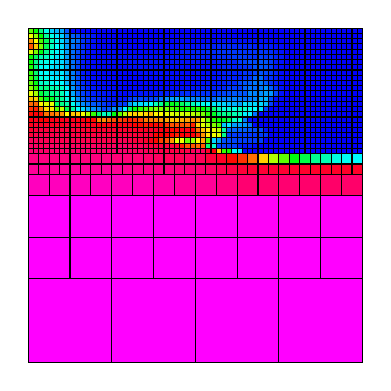
\begin{tikzpicture}[x={(.35\textwidth,0)},y={(0,.35\textwidth)}]
        \def\initiallinewidth{0.4pt}
\definecolor{fillcolor}{rgb}{1.000000,0.000000,1.000000}
\fill[fillcolor] (0.000000,0.000000) rectangle (0.250000,0.250000);
\definecolor{fillcolor}{rgb}{1.000000,0.000000,1.000000}
\fill[fillcolor] (0.250000,0.000000) rectangle (0.500000,0.250000);
\definecolor{fillcolor}{rgb}{1.000000,0.000000,1.000000}
\fill[fillcolor] (0.000000,0.250000) rectangle (0.125000,0.375000);
\definecolor{fillcolor}{rgb}{1.000000,0.000000,1.000000}
\fill[fillcolor] (0.125000,0.250000) rectangle (0.250000,0.375000);
\definecolor{fillcolor}{rgb}{1.000000,0.000000,1.000000}
\fill[fillcolor] (0.000000,0.375000) rectangle (0.125000,0.500000);
\definecolor{fillcolor}{rgb}{1.000000,0.000000,1.000000}
\fill[fillcolor] (0.125000,0.375000) rectangle (0.250000,0.500000);
\definecolor{fillcolor}{rgb}{1.000000,0.000000,1.000000}
\fill[fillcolor] (0.250000,0.250000) rectangle (0.375000,0.375000);
\definecolor{fillcolor}{rgb}{1.000000,0.000000,1.000000}
\fill[fillcolor] (0.375000,0.250000) rectangle (0.500000,0.375000);
\definecolor{fillcolor}{rgb}{1.000000,0.000000,1.000000}
\fill[fillcolor] (0.250000,0.375000) rectangle (0.375000,0.500000);
\definecolor{fillcolor}{rgb}{1.000000,0.000000,1.000000}
\fill[fillcolor] (0.375000,0.375000) rectangle (0.500000,0.500000);
\definecolor{fillcolor}{rgb}{1.000000,0.000000,1.000000}
\fill[fillcolor] (0.500000,0.000000) rectangle (0.750000,0.250000);
\definecolor{fillcolor}{rgb}{1.000000,0.000000,1.000000}
\fill[fillcolor] (0.750000,0.000000) rectangle (1.000000,0.250000);
\definecolor{fillcolor}{rgb}{1.000000,0.000000,1.000000}
\fill[fillcolor] (0.500000,0.250000) rectangle (0.625000,0.375000);
\definecolor{fillcolor}{rgb}{1.000000,0.000000,1.000000}
\fill[fillcolor] (0.625000,0.250000) rectangle (0.750000,0.375000);
\definecolor{fillcolor}{rgb}{1.000000,0.000000,1.000000}
\fill[fillcolor] (0.500000,0.375000) rectangle (0.625000,0.500000);
\definecolor{fillcolor}{rgb}{1.000000,0.000000,0.973407}
\fill[fillcolor] (0.625000,0.375000) rectangle (0.750000,0.500000);
\definecolor{fillcolor}{rgb}{1.000000,0.000000,1.000000}
\fill[fillcolor] (0.750000,0.250000) rectangle (0.875000,0.375000);
\definecolor{fillcolor}{rgb}{1.000000,0.000000,1.000000}
\fill[fillcolor] (0.875000,0.250000) rectangle (1.000000,0.375000);
\definecolor{fillcolor}{rgb}{1.000000,0.000000,0.967010}
\fill[fillcolor] (0.750000,0.375000) rectangle (0.875000,0.500000);
\definecolor{fillcolor}{rgb}{1.000000,0.000000,0.983925}
\fill[fillcolor] (0.875000,0.375000) rectangle (1.000000,0.500000);
\definecolor{fillcolor}{rgb}{1.000000,0.000000,0.746577}
\fill[fillcolor] (0.000000,0.500000) rectangle (0.062500,0.562500);
\definecolor{fillcolor}{rgb}{1.000000,0.000000,0.736508}
\fill[fillcolor] (0.062500,0.500000) rectangle (0.125000,0.562500);
\definecolor{fillcolor}{rgb}{1.000000,0.000000,0.599750}
\fill[fillcolor] (0.000000,0.562500) rectangle (0.031250,0.593750);
\definecolor{fillcolor}{rgb}{1.000000,0.000000,0.599327}
\fill[fillcolor] (0.031250,0.562500) rectangle (0.062500,0.593750);
\definecolor{fillcolor}{rgb}{1.000000,0.000000,0.512768}
\fill[fillcolor] (0.000000,0.593750) rectangle (0.031250,0.625000);
\definecolor{fillcolor}{rgb}{1.000000,0.000000,0.511668}
\fill[fillcolor] (0.031250,0.593750) rectangle (0.062500,0.625000);
\definecolor{fillcolor}{rgb}{1.000000,0.000000,0.591451}
\fill[fillcolor] (0.062500,0.562500) rectangle (0.093750,0.593750);
\definecolor{fillcolor}{rgb}{1.000000,0.000000,0.608837}
\fill[fillcolor] (0.093750,0.562500) rectangle (0.125000,0.593750);
\definecolor{fillcolor}{rgb}{1.000000,0.000000,0.502720}
\fill[fillcolor] (0.062500,0.593750) rectangle (0.093750,0.625000);
\definecolor{fillcolor}{rgb}{1.000000,0.000000,0.506204}
\fill[fillcolor] (0.093750,0.593750) rectangle (0.125000,0.625000);
\definecolor{fillcolor}{rgb}{1.000000,0.000000,0.748243}
\fill[fillcolor] (0.125000,0.500000) rectangle (0.187500,0.562500);
\definecolor{fillcolor}{rgb}{1.000000,0.000000,0.758200}
\fill[fillcolor] (0.187500,0.500000) rectangle (0.250000,0.562500);
\definecolor{fillcolor}{rgb}{1.000000,0.000000,0.604355}
\fill[fillcolor] (0.125000,0.562500) rectangle (0.156250,0.593750);
\definecolor{fillcolor}{rgb}{1.000000,0.000000,0.578468}
\fill[fillcolor] (0.156250,0.562500) rectangle (0.187500,0.593750);
\definecolor{fillcolor}{rgb}{1.000000,0.000000,0.508096}
\fill[fillcolor] (0.125000,0.593750) rectangle (0.156250,0.625000);
\definecolor{fillcolor}{rgb}{1.000000,0.000000,0.490625}
\fill[fillcolor] (0.156250,0.593750) rectangle (0.187500,0.625000);
\definecolor{fillcolor}{rgb}{1.000000,0.000000,0.580919}
\fill[fillcolor] (0.187500,0.562500) rectangle (0.218750,0.593750);
\definecolor{fillcolor}{rgb}{1.000000,0.000000,0.596826}
\fill[fillcolor] (0.218750,0.562500) rectangle (0.250000,0.593750);
\definecolor{fillcolor}{rgb}{1.000000,0.000000,0.499816}
\fill[fillcolor] (0.187500,0.593750) rectangle (0.218750,0.625000);
\definecolor{fillcolor}{rgb}{1.000000,0.000000,0.506208}
\fill[fillcolor] (0.218750,0.593750) rectangle (0.250000,0.625000);
\definecolor{fillcolor}{rgb}{1.000000,0.000000,0.452281}
\fill[fillcolor] (0.000000,0.625000) rectangle (0.015625,0.640625);
\definecolor{fillcolor}{rgb}{1.000000,0.000000,0.452714}
\fill[fillcolor] (0.015625,0.625000) rectangle (0.031250,0.640625);
\definecolor{fillcolor}{rgb}{1.000000,0.000000,0.406395}
\fill[fillcolor] (0.000000,0.640625) rectangle (0.015625,0.656250);
\definecolor{fillcolor}{rgb}{1.000000,0.000000,0.410049}
\fill[fillcolor] (0.015625,0.640625) rectangle (0.031250,0.656250);
\definecolor{fillcolor}{rgb}{1.000000,0.000000,0.414603}
\fill[fillcolor] (0.031250,0.625000) rectangle (0.046875,0.640625);
\definecolor{fillcolor}{rgb}{1.000000,0.000000,0.416782}
\fill[fillcolor] (0.046875,0.625000) rectangle (0.062500,0.640625);
\definecolor{fillcolor}{rgb}{1.000000,0.000000,0.338345}
\fill[fillcolor] (0.031250,0.640625) rectangle (0.046875,0.656250);
\definecolor{fillcolor}{rgb}{1.000000,0.000000,0.373404}
\fill[fillcolor] (0.046875,0.640625) rectangle (0.062500,0.656250);
\definecolor{fillcolor}{rgb}{1.000000,0.000000,0.365071}
\fill[fillcolor] (0.000000,0.656250) rectangle (0.015625,0.671875);
\definecolor{fillcolor}{rgb}{1.000000,0.000000,0.363928}
\fill[fillcolor] (0.015625,0.656250) rectangle (0.031250,0.671875);
\definecolor{fillcolor}{rgb}{1.000000,0.000000,0.225830}
\fill[fillcolor] (0.000000,0.671875) rectangle (0.015625,0.687500);
\definecolor{fillcolor}{rgb}{1.000000,0.000000,0.299114}
\fill[fillcolor] (0.015625,0.671875) rectangle (0.031250,0.687500);
\definecolor{fillcolor}{rgb}{1.000000,0.000000,0.344013}
\fill[fillcolor] (0.031250,0.656250) rectangle (0.046875,0.671875);
\definecolor{fillcolor}{rgb}{1.000000,0.000000,0.329832}
\fill[fillcolor] (0.046875,0.656250) rectangle (0.062500,0.671875);
\definecolor{fillcolor}{rgb}{1.000000,0.000000,0.298793}
\fill[fillcolor] (0.031250,0.671875) rectangle (0.046875,0.687500);
\definecolor{fillcolor}{rgb}{1.000000,0.000000,0.294624}
\fill[fillcolor] (0.046875,0.671875) rectangle (0.062500,0.687500);
\definecolor{fillcolor}{rgb}{1.000000,0.000000,0.432165}
\fill[fillcolor] (0.062500,0.625000) rectangle (0.078125,0.640625);
\definecolor{fillcolor}{rgb}{1.000000,0.000000,0.440253}
\fill[fillcolor] (0.078125,0.625000) rectangle (0.093750,0.640625);
\definecolor{fillcolor}{rgb}{1.000000,0.000000,0.397112}
\fill[fillcolor] (0.062500,0.640625) rectangle (0.078125,0.656250);
\definecolor{fillcolor}{rgb}{1.000000,0.000000,0.399312}
\fill[fillcolor] (0.078125,0.640625) rectangle (0.093750,0.656250);
\definecolor{fillcolor}{rgb}{1.000000,0.000000,0.429768}
\fill[fillcolor] (0.093750,0.625000) rectangle (0.109375,0.640625);
\definecolor{fillcolor}{rgb}{1.000000,0.000000,0.430106}
\fill[fillcolor] (0.109375,0.625000) rectangle (0.125000,0.640625);
\definecolor{fillcolor}{rgb}{1.000000,0.000000,0.371671}
\fill[fillcolor] (0.093750,0.640625) rectangle (0.109375,0.656250);
\definecolor{fillcolor}{rgb}{1.000000,0.000000,0.365898}
\fill[fillcolor] (0.109375,0.640625) rectangle (0.125000,0.656250);
\definecolor{fillcolor}{rgb}{1.000000,0.000000,0.338913}
\fill[fillcolor] (0.062500,0.656250) rectangle (0.078125,0.671875);
\definecolor{fillcolor}{rgb}{1.000000,0.000000,0.349497}
\fill[fillcolor] (0.078125,0.656250) rectangle (0.093750,0.671875);
\definecolor{fillcolor}{rgb}{1.000000,0.000000,0.292570}
\fill[fillcolor] (0.062500,0.671875) rectangle (0.078125,0.687500);
\definecolor{fillcolor}{rgb}{1.000000,0.000000,0.308763}
\fill[fillcolor] (0.078125,0.671875) rectangle (0.093750,0.687500);
\definecolor{fillcolor}{rgb}{1.000000,0.000000,0.314383}
\fill[fillcolor] (0.093750,0.656250) rectangle (0.109375,0.671875);
\definecolor{fillcolor}{rgb}{1.000000,0.000000,0.322536}
\fill[fillcolor] (0.109375,0.656250) rectangle (0.125000,0.671875);
\definecolor{fillcolor}{rgb}{1.000000,0.000000,0.297727}
\fill[fillcolor] (0.093750,0.671875) rectangle (0.109375,0.687500);
\definecolor{fillcolor}{rgb}{1.000000,0.000000,0.289849}
\fill[fillcolor] (0.109375,0.671875) rectangle (0.125000,0.687500);
\definecolor{fillcolor}{rgb}{1.000000,0.000000,0.173699}
\fill[fillcolor] (0.000000,0.687500) rectangle (0.015625,0.703125);
\definecolor{fillcolor}{rgb}{1.000000,0.000000,0.231016}
\fill[fillcolor] (0.015625,0.687500) rectangle (0.031250,0.703125);
\definecolor{fillcolor}{rgb}{1.000000,0.000000,0.115917}
\fill[fillcolor] (0.000000,0.703125) rectangle (0.015625,0.718750);
\definecolor{fillcolor}{rgb}{1.000000,0.000000,0.179824}
\fill[fillcolor] (0.015625,0.703125) rectangle (0.031250,0.718750);
\definecolor{fillcolor}{rgb}{1.000000,0.000000,0.244124}
\fill[fillcolor] (0.031250,0.687500) rectangle (0.046875,0.703125);
\definecolor{fillcolor}{rgb}{1.000000,0.000000,0.237896}
\fill[fillcolor] (0.046875,0.687500) rectangle (0.062500,0.703125);
\definecolor{fillcolor}{rgb}{1.000000,0.000000,0.155796}
\fill[fillcolor] (0.031250,0.703125) rectangle (0.046875,0.718750);
\definecolor{fillcolor}{rgb}{1.000000,0.000000,0.146004}
\fill[fillcolor] (0.046875,0.703125) rectangle (0.062500,0.718750);
\definecolor{fillcolor}{rgb}{1.000000,0.000000,0.051154}
\fill[fillcolor] (0.000000,0.718750) rectangle (0.015625,0.734375);
\definecolor{fillcolor}{rgb}{1.000000,0.000000,0.114547}
\fill[fillcolor] (0.015625,0.718750) rectangle (0.031250,0.734375);
\definecolor{fillcolor}{rgb}{1.000000,0.045635,0.000000}
\fill[fillcolor] (0.000000,0.734375) rectangle (0.015625,0.750000);
\definecolor{fillcolor}{rgb}{1.000000,0.000000,0.026961}
\fill[fillcolor] (0.015625,0.734375) rectangle (0.031250,0.750000);
\definecolor{fillcolor}{rgb}{1.000000,0.002278,0.000000}
\fill[fillcolor] (0.031250,0.718750) rectangle (0.046875,0.734375);
\definecolor{fillcolor}{rgb}{1.000000,0.000000,0.018083}
\fill[fillcolor] (0.046875,0.718750) rectangle (0.062500,0.734375);
\definecolor{fillcolor}{rgb}{1.000000,0.086244,0.000000}
\fill[fillcolor] (0.031250,0.734375) rectangle (0.046875,0.750000);
\definecolor{fillcolor}{rgb}{1.000000,0.453283,0.000000}
\fill[fillcolor] (0.046875,0.734375) rectangle (0.062500,0.750000);
\definecolor{fillcolor}{rgb}{1.000000,0.000000,0.243491}
\fill[fillcolor] (0.062500,0.687500) rectangle (0.078125,0.703125);
\definecolor{fillcolor}{rgb}{1.000000,0.000000,0.252331}
\fill[fillcolor] (0.078125,0.687500) rectangle (0.093750,0.703125);
\definecolor{fillcolor}{rgb}{1.000000,0.000000,0.148317}
\fill[fillcolor] (0.062500,0.703125) rectangle (0.078125,0.718750);
\definecolor{fillcolor}{rgb}{1.000000,0.000000,0.142754}
\fill[fillcolor] (0.078125,0.703125) rectangle (0.093750,0.718750);
\definecolor{fillcolor}{rgb}{1.000000,0.000000,0.247834}
\fill[fillcolor] (0.093750,0.687500) rectangle (0.109375,0.703125);
\definecolor{fillcolor}{rgb}{1.000000,0.000000,0.246056}
\fill[fillcolor] (0.109375,0.687500) rectangle (0.125000,0.703125);
\definecolor{fillcolor}{rgb}{1.000000,0.000000,0.134438}
\fill[fillcolor] (0.093750,0.703125) rectangle (0.109375,0.718750);
\definecolor{fillcolor}{rgb}{1.000000,0.000000,0.194303}
\fill[fillcolor] (0.109375,0.703125) rectangle (0.125000,0.718750);
\definecolor{fillcolor}{rgb}{1.000000,0.000000,0.081207}
\fill[fillcolor] (0.062500,0.718750) rectangle (0.078125,0.734375);
\definecolor{fillcolor}{rgb}{1.000000,0.000000,0.085287}
\fill[fillcolor] (0.078125,0.718750) rectangle (0.093750,0.734375);
\definecolor{fillcolor}{rgb}{1.000000,0.441379,0.000000}
\fill[fillcolor] (0.062500,0.734375) rectangle (0.078125,0.750000);
\definecolor{fillcolor}{rgb}{1.000000,0.538328,0.000000}
\fill[fillcolor] (0.078125,0.734375) rectangle (0.093750,0.750000);
\definecolor{fillcolor}{rgb}{1.000000,0.000000,0.094756}
\fill[fillcolor] (0.093750,0.718750) rectangle (0.109375,0.734375);
\definecolor{fillcolor}{rgb}{1.000000,0.000000,0.122622}
\fill[fillcolor] (0.109375,0.718750) rectangle (0.125000,0.734375);
\definecolor{fillcolor}{rgb}{1.000000,0.586219,0.000000}
\fill[fillcolor] (0.093750,0.734375) rectangle (0.109375,0.750000);
\definecolor{fillcolor}{rgb}{0.998173,1.000000,0.000000}
\fill[fillcolor] (0.109375,0.734375) rectangle (0.125000,0.750000);
\definecolor{fillcolor}{rgb}{1.000000,0.000000,0.429235}
\fill[fillcolor] (0.125000,0.625000) rectangle (0.140625,0.640625);
\definecolor{fillcolor}{rgb}{1.000000,0.000000,0.427533}
\fill[fillcolor] (0.140625,0.625000) rectangle (0.156250,0.640625);
\definecolor{fillcolor}{rgb}{1.000000,0.000000,0.369341}
\fill[fillcolor] (0.125000,0.640625) rectangle (0.140625,0.656250);
\definecolor{fillcolor}{rgb}{1.000000,0.000000,0.373001}
\fill[fillcolor] (0.140625,0.640625) rectangle (0.156250,0.656250);
\definecolor{fillcolor}{rgb}{1.000000,0.000000,0.426320}
\fill[fillcolor] (0.156250,0.625000) rectangle (0.171875,0.640625);
\definecolor{fillcolor}{rgb}{1.000000,0.000000,0.431297}
\fill[fillcolor] (0.171875,0.625000) rectangle (0.187500,0.640625);
\definecolor{fillcolor}{rgb}{1.000000,0.000000,0.369892}
\fill[fillcolor] (0.156250,0.640625) rectangle (0.171875,0.656250);
\definecolor{fillcolor}{rgb}{1.000000,0.000000,0.373869}
\fill[fillcolor] (0.171875,0.640625) rectangle (0.187500,0.656250);
\definecolor{fillcolor}{rgb}{1.000000,0.000000,0.320340}
\fill[fillcolor] (0.125000,0.656250) rectangle (0.140625,0.671875);
\definecolor{fillcolor}{rgb}{1.000000,0.000000,0.321132}
\fill[fillcolor] (0.140625,0.656250) rectangle (0.156250,0.671875);
\definecolor{fillcolor}{rgb}{1.000000,0.000000,0.270048}
\fill[fillcolor] (0.125000,0.671875) rectangle (0.140625,0.687500);
\definecolor{fillcolor}{rgb}{1.000000,0.000000,0.261938}
\fill[fillcolor] (0.140625,0.671875) rectangle (0.156250,0.687500);
\definecolor{fillcolor}{rgb}{1.000000,0.000000,0.313494}
\fill[fillcolor] (0.156250,0.656250) rectangle (0.171875,0.671875);
\definecolor{fillcolor}{rgb}{1.000000,0.000000,0.310706}
\fill[fillcolor] (0.171875,0.656250) rectangle (0.187500,0.671875);
\definecolor{fillcolor}{rgb}{1.000000,0.000000,0.253075}
\fill[fillcolor] (0.156250,0.671875) rectangle (0.171875,0.687500);
\definecolor{fillcolor}{rgb}{1.000000,0.000000,0.255256}
\fill[fillcolor] (0.171875,0.671875) rectangle (0.187500,0.687500);
\definecolor{fillcolor}{rgb}{1.000000,0.000000,0.438637}
\fill[fillcolor] (0.187500,0.625000) rectangle (0.203125,0.640625);
\definecolor{fillcolor}{rgb}{1.000000,0.000000,0.435730}
\fill[fillcolor] (0.203125,0.625000) rectangle (0.218750,0.640625);
\definecolor{fillcolor}{rgb}{1.000000,0.000000,0.387681}
\fill[fillcolor] (0.187500,0.640625) rectangle (0.203125,0.656250);
\definecolor{fillcolor}{rgb}{1.000000,0.000000,0.384578}
\fill[fillcolor] (0.203125,0.640625) rectangle (0.218750,0.656250);
\definecolor{fillcolor}{rgb}{1.000000,0.000000,0.432412}
\fill[fillcolor] (0.218750,0.625000) rectangle (0.234375,0.640625);
\definecolor{fillcolor}{rgb}{1.000000,0.000000,0.429825}
\fill[fillcolor] (0.234375,0.625000) rectangle (0.250000,0.640625);
\definecolor{fillcolor}{rgb}{1.000000,0.000000,0.370174}
\fill[fillcolor] (0.218750,0.640625) rectangle (0.234375,0.656250);
\definecolor{fillcolor}{rgb}{1.000000,0.000000,0.361179}
\fill[fillcolor] (0.234375,0.640625) rectangle (0.250000,0.656250);
\definecolor{fillcolor}{rgb}{1.000000,0.000000,0.321873}
\fill[fillcolor] (0.187500,0.656250) rectangle (0.203125,0.671875);
\definecolor{fillcolor}{rgb}{1.000000,0.000000,0.329579}
\fill[fillcolor] (0.203125,0.656250) rectangle (0.218750,0.671875);
\definecolor{fillcolor}{rgb}{1.000000,0.000000,0.258797}
\fill[fillcolor] (0.187500,0.671875) rectangle (0.203125,0.687500);
\definecolor{fillcolor}{rgb}{1.000000,0.000000,0.269175}
\fill[fillcolor] (0.203125,0.671875) rectangle (0.218750,0.687500);
\definecolor{fillcolor}{rgb}{1.000000,0.000000,0.308432}
\fill[fillcolor] (0.218750,0.656250) rectangle (0.234375,0.671875);
\definecolor{fillcolor}{rgb}{1.000000,0.000000,0.292583}
\fill[fillcolor] (0.234375,0.656250) rectangle (0.250000,0.671875);
\definecolor{fillcolor}{rgb}{1.000000,0.000000,0.260583}
\fill[fillcolor] (0.218750,0.671875) rectangle (0.234375,0.687500);
\definecolor{fillcolor}{rgb}{1.000000,0.000000,0.240064}
\fill[fillcolor] (0.234375,0.671875) rectangle (0.250000,0.687500);
\definecolor{fillcolor}{rgb}{1.000000,0.000000,0.232287}
\fill[fillcolor] (0.125000,0.687500) rectangle (0.140625,0.703125);
\definecolor{fillcolor}{rgb}{1.000000,0.000000,0.220103}
\fill[fillcolor] (0.140625,0.687500) rectangle (0.156250,0.703125);
\definecolor{fillcolor}{rgb}{1.000000,0.000000,0.183404}
\fill[fillcolor] (0.125000,0.703125) rectangle (0.140625,0.718750);
\definecolor{fillcolor}{rgb}{1.000000,0.000000,0.154017}
\fill[fillcolor] (0.140625,0.703125) rectangle (0.156250,0.718750);
\definecolor{fillcolor}{rgb}{1.000000,0.000000,0.202477}
\fill[fillcolor] (0.156250,0.687500) rectangle (0.171875,0.703125);
\definecolor{fillcolor}{rgb}{1.000000,0.000000,0.190761}
\fill[fillcolor] (0.171875,0.687500) rectangle (0.187500,0.703125);
\definecolor{fillcolor}{rgb}{1.000000,0.000000,0.154424}
\fill[fillcolor] (0.156250,0.703125) rectangle (0.171875,0.718750);
\definecolor{fillcolor}{rgb}{1.000000,0.000000,0.112734}
\fill[fillcolor] (0.171875,0.703125) rectangle (0.187500,0.718750);
\definecolor{fillcolor}{rgb}{1.000000,0.000000,0.106653}
\fill[fillcolor] (0.125000,0.718750) rectangle (0.140625,0.734375);
\definecolor{fillcolor}{rgb}{1.000000,0.000000,0.072196}
\fill[fillcolor] (0.140625,0.718750) rectangle (0.156250,0.734375);
\definecolor{fillcolor}{rgb}{1.000000,0.770793,0.000000}
\fill[fillcolor] (0.125000,0.734375) rectangle (0.140625,0.750000);
\definecolor{fillcolor}{rgb}{1.000000,0.809160,0.000000}
\fill[fillcolor] (0.140625,0.734375) rectangle (0.156250,0.750000);
\definecolor{fillcolor}{rgb}{1.000000,0.000000,0.065863}
\fill[fillcolor] (0.156250,0.718750) rectangle (0.171875,0.734375);
\definecolor{fillcolor}{rgb}{1.000000,0.000000,0.009906}
\fill[fillcolor] (0.171875,0.718750) rectangle (0.187500,0.734375);
\definecolor{fillcolor}{rgb}{0.978524,1.000000,0.000000}
\fill[fillcolor] (0.156250,0.734375) rectangle (0.171875,0.750000);
\definecolor{fillcolor}{rgb}{0.687288,1.000000,0.000000}
\fill[fillcolor] (0.171875,0.734375) rectangle (0.187500,0.750000);
\definecolor{fillcolor}{rgb}{1.000000,0.000000,0.175291}
\fill[fillcolor] (0.187500,0.687500) rectangle (0.203125,0.703125);
\definecolor{fillcolor}{rgb}{1.000000,0.000000,0.189429}
\fill[fillcolor] (0.203125,0.687500) rectangle (0.218750,0.703125);
\definecolor{fillcolor}{rgb}{1.000000,0.000000,0.105987}
\fill[fillcolor] (0.187500,0.703125) rectangle (0.203125,0.718750);
\definecolor{fillcolor}{rgb}{1.000000,0.000000,0.037351}
\fill[fillcolor] (0.203125,0.703125) rectangle (0.218750,0.718750);
\definecolor{fillcolor}{rgb}{1.000000,0.000000,0.197319}
\fill[fillcolor] (0.218750,0.687500) rectangle (0.234375,0.703125);
\definecolor{fillcolor}{rgb}{1.000000,0.000000,0.194246}
\fill[fillcolor] (0.234375,0.687500) rectangle (0.250000,0.703125);
\definecolor{fillcolor}{rgb}{1.000000,0.000000,0.071174}
\fill[fillcolor] (0.218750,0.703125) rectangle (0.234375,0.718750);
\definecolor{fillcolor}{rgb}{1.000000,0.000000,0.079739}
\fill[fillcolor] (0.234375,0.703125) rectangle (0.250000,0.718750);
\definecolor{fillcolor}{rgb}{1.000000,0.044118,0.000000}
\fill[fillcolor] (0.187500,0.718750) rectangle (0.203125,0.734375);
\definecolor{fillcolor}{rgb}{1.000000,0.534658,0.000000}
\fill[fillcolor] (0.203125,0.718750) rectangle (0.218750,0.734375);
\definecolor{fillcolor}{rgb}{0.195553,1.000000,0.000000}
\fill[fillcolor] (0.187500,0.734375) rectangle (0.203125,0.750000);
\definecolor{fillcolor}{rgb}{0.000000,1.000000,0.391611}
\fill[fillcolor] (0.203125,0.734375) rectangle (0.218750,0.750000);
\definecolor{fillcolor}{rgb}{1.000000,0.549750,0.000000}
\fill[fillcolor] (0.218750,0.718750) rectangle (0.234375,0.734375);
\definecolor{fillcolor}{rgb}{1.000000,0.413625,0.000000}
\fill[fillcolor] (0.234375,0.718750) rectangle (0.250000,0.734375);
\definecolor{fillcolor}{rgb}{0.000000,1.000000,0.758559}
\fill[fillcolor] (0.218750,0.734375) rectangle (0.234375,0.750000);
\definecolor{fillcolor}{rgb}{0.000000,1.000000,0.697042}
\fill[fillcolor] (0.234375,0.734375) rectangle (0.250000,0.750000);
\definecolor{fillcolor}{rgb}{1.000000,0.000000,0.741345}
\fill[fillcolor] (0.250000,0.500000) rectangle (0.312500,0.562500);
\definecolor{fillcolor}{rgb}{1.000000,0.000000,0.732795}
\fill[fillcolor] (0.312500,0.500000) rectangle (0.375000,0.562500);
\definecolor{fillcolor}{rgb}{1.000000,0.000000,0.587610}
\fill[fillcolor] (0.250000,0.562500) rectangle (0.281250,0.593750);
\definecolor{fillcolor}{rgb}{1.000000,0.000000,0.551935}
\fill[fillcolor] (0.281250,0.562500) rectangle (0.312500,0.593750);
\definecolor{fillcolor}{rgb}{1.000000,0.000000,0.470319}
\fill[fillcolor] (0.250000,0.593750) rectangle (0.281250,0.625000);
\definecolor{fillcolor}{rgb}{1.000000,0.000000,0.466140}
\fill[fillcolor] (0.281250,0.593750) rectangle (0.312500,0.625000);
\definecolor{fillcolor}{rgb}{1.000000,0.000000,0.531617}
\fill[fillcolor] (0.312500,0.562500) rectangle (0.343750,0.593750);
\definecolor{fillcolor}{rgb}{1.000000,0.000000,0.531082}
\fill[fillcolor] (0.343750,0.562500) rectangle (0.375000,0.593750);
\definecolor{fillcolor}{rgb}{1.000000,0.000000,0.460665}
\fill[fillcolor] (0.312500,0.593750) rectangle (0.343750,0.625000);
\definecolor{fillcolor}{rgb}{1.000000,0.000000,0.416920}
\fill[fillcolor] (0.343750,0.593750) rectangle (0.375000,0.625000);
\definecolor{fillcolor}{rgb}{1.000000,0.000000,0.682132}
\fill[fillcolor] (0.375000,0.500000) rectangle (0.437500,0.562500);
\definecolor{fillcolor}{rgb}{1.000000,0.000000,0.619526}
\fill[fillcolor] (0.437500,0.500000) rectangle (0.500000,0.562500);
\definecolor{fillcolor}{rgb}{1.000000,0.000000,0.501169}
\fill[fillcolor] (0.375000,0.562500) rectangle (0.406250,0.593750);
\definecolor{fillcolor}{rgb}{1.000000,0.000000,0.488953}
\fill[fillcolor] (0.406250,0.562500) rectangle (0.437500,0.593750);
\definecolor{fillcolor}{rgb}{1.000000,0.000000,0.386158}
\fill[fillcolor] (0.375000,0.593750) rectangle (0.406250,0.625000);
\definecolor{fillcolor}{rgb}{1.000000,0.000000,0.350099}
\fill[fillcolor] (0.406250,0.593750) rectangle (0.437500,0.625000);
\definecolor{fillcolor}{rgb}{1.000000,0.000000,0.462525}
\fill[fillcolor] (0.437500,0.562500) rectangle (0.468750,0.593750);
\definecolor{fillcolor}{rgb}{1.000000,0.000000,0.455596}
\fill[fillcolor] (0.468750,0.562500) rectangle (0.500000,0.593750);
\definecolor{fillcolor}{rgb}{1.000000,0.000000,0.332215}
\fill[fillcolor] (0.437500,0.593750) rectangle (0.468750,0.625000);
\definecolor{fillcolor}{rgb}{1.000000,0.000000,0.383348}
\fill[fillcolor] (0.468750,0.593750) rectangle (0.500000,0.625000);
\definecolor{fillcolor}{rgb}{1.000000,0.000000,0.435170}
\fill[fillcolor] (0.250000,0.625000) rectangle (0.265625,0.640625);
\definecolor{fillcolor}{rgb}{1.000000,0.000000,0.432600}
\fill[fillcolor] (0.265625,0.625000) rectangle (0.281250,0.640625);
\definecolor{fillcolor}{rgb}{1.000000,0.000000,0.382940}
\fill[fillcolor] (0.250000,0.640625) rectangle (0.265625,0.656250);
\definecolor{fillcolor}{rgb}{1.000000,0.000000,0.406289}
\fill[fillcolor] (0.265625,0.640625) rectangle (0.281250,0.656250);
\definecolor{fillcolor}{rgb}{1.000000,0.000000,0.423182}
\fill[fillcolor] (0.281250,0.625000) rectangle (0.296875,0.640625);
\definecolor{fillcolor}{rgb}{1.000000,0.000000,0.403421}
\fill[fillcolor] (0.296875,0.625000) rectangle (0.312500,0.640625);
\definecolor{fillcolor}{rgb}{1.000000,0.000000,0.402722}
\fill[fillcolor] (0.281250,0.640625) rectangle (0.296875,0.656250);
\definecolor{fillcolor}{rgb}{1.000000,0.000000,0.372985}
\fill[fillcolor] (0.296875,0.640625) rectangle (0.312500,0.656250);
\definecolor{fillcolor}{rgb}{1.000000,0.000000,0.307910}
\fill[fillcolor] (0.250000,0.656250) rectangle (0.265625,0.671875);
\definecolor{fillcolor}{rgb}{1.000000,0.000000,0.331464}
\fill[fillcolor] (0.265625,0.656250) rectangle (0.281250,0.671875);
\definecolor{fillcolor}{rgb}{1.000000,0.000000,0.233395}
\fill[fillcolor] (0.250000,0.671875) rectangle (0.265625,0.687500);
\definecolor{fillcolor}{rgb}{1.000000,0.000000,0.240728}
\fill[fillcolor] (0.265625,0.671875) rectangle (0.281250,0.687500);
\definecolor{fillcolor}{rgb}{1.000000,0.000000,0.331310}
\fill[fillcolor] (0.281250,0.656250) rectangle (0.296875,0.671875);
\definecolor{fillcolor}{rgb}{1.000000,0.000000,0.293312}
\fill[fillcolor] (0.296875,0.656250) rectangle (0.312500,0.671875);
\definecolor{fillcolor}{rgb}{1.000000,0.000000,0.252810}
\fill[fillcolor] (0.281250,0.671875) rectangle (0.296875,0.687500);
\definecolor{fillcolor}{rgb}{1.000000,0.000000,0.243865}
\fill[fillcolor] (0.296875,0.671875) rectangle (0.312500,0.687500);
\definecolor{fillcolor}{rgb}{1.000000,0.000000,0.372647}
\fill[fillcolor] (0.312500,0.625000) rectangle (0.328125,0.640625);
\definecolor{fillcolor}{rgb}{1.000000,0.000000,0.378745}
\fill[fillcolor] (0.328125,0.625000) rectangle (0.343750,0.640625);
\definecolor{fillcolor}{rgb}{1.000000,0.000000,0.335647}
\fill[fillcolor] (0.312500,0.640625) rectangle (0.328125,0.656250);
\definecolor{fillcolor}{rgb}{1.000000,0.000000,0.358679}
\fill[fillcolor] (0.328125,0.640625) rectangle (0.343750,0.656250);
\definecolor{fillcolor}{rgb}{1.000000,0.000000,0.357512}
\fill[fillcolor] (0.343750,0.625000) rectangle (0.359375,0.640625);
\definecolor{fillcolor}{rgb}{1.000000,0.000000,0.339815}
\fill[fillcolor] (0.359375,0.625000) rectangle (0.375000,0.640625);
\definecolor{fillcolor}{rgb}{1.000000,0.000000,0.328219}
\fill[fillcolor] (0.343750,0.640625) rectangle (0.359375,0.656250);
\definecolor{fillcolor}{rgb}{1.000000,0.000000,0.262520}
\fill[fillcolor] (0.359375,0.640625) rectangle (0.375000,0.656250);
\definecolor{fillcolor}{rgb}{1.000000,0.000000,0.239234}
\fill[fillcolor] (0.312500,0.656250) rectangle (0.328125,0.671875);
\definecolor{fillcolor}{rgb}{1.000000,0.000000,0.238403}
\fill[fillcolor] (0.328125,0.656250) rectangle (0.343750,0.671875);
\definecolor{fillcolor}{rgb}{1.000000,0.000000,0.218215}
\fill[fillcolor] (0.312500,0.671875) rectangle (0.328125,0.687500);
\definecolor{fillcolor}{rgb}{1.000000,0.000000,0.215468}
\fill[fillcolor] (0.328125,0.671875) rectangle (0.343750,0.687500);
\definecolor{fillcolor}{rgb}{1.000000,0.000000,0.171382}
\fill[fillcolor] (0.343750,0.656250) rectangle (0.359375,0.671875);
\definecolor{fillcolor}{rgb}{1.000000,0.000000,0.102330}
\fill[fillcolor] (0.359375,0.656250) rectangle (0.375000,0.671875);
\definecolor{fillcolor}{rgb}{1.000000,0.000000,0.237987}
\fill[fillcolor] (0.343750,0.671875) rectangle (0.359375,0.687500);
\definecolor{fillcolor}{rgb}{1.000000,0.000000,0.189982}
\fill[fillcolor] (0.359375,0.671875) rectangle (0.375000,0.687500);
\definecolor{fillcolor}{rgb}{1.000000,0.000000,0.186552}
\fill[fillcolor] (0.250000,0.687500) rectangle (0.265625,0.703125);
\definecolor{fillcolor}{rgb}{1.000000,0.000000,0.179321}
\fill[fillcolor] (0.265625,0.687500) rectangle (0.281250,0.703125);
\definecolor{fillcolor}{rgb}{1.000000,0.000000,0.083635}
\fill[fillcolor] (0.250000,0.703125) rectangle (0.265625,0.718750);
\definecolor{fillcolor}{rgb}{1.000000,0.000000,0.088110}
\fill[fillcolor] (0.265625,0.703125) rectangle (0.281250,0.718750);
\definecolor{fillcolor}{rgb}{1.000000,0.000000,0.183441}
\fill[fillcolor] (0.281250,0.687500) rectangle (0.296875,0.703125);
\definecolor{fillcolor}{rgb}{1.000000,0.000000,0.171615}
\fill[fillcolor] (0.296875,0.687500) rectangle (0.312500,0.703125);
\definecolor{fillcolor}{rgb}{1.000000,0.000000,0.081042}
\fill[fillcolor] (0.281250,0.703125) rectangle (0.296875,0.718750);
\definecolor{fillcolor}{rgb}{1.000000,0.000000,0.085790}
\fill[fillcolor] (0.296875,0.703125) rectangle (0.312500,0.718750);
\definecolor{fillcolor}{rgb}{1.000000,0.298699,0.000000}
\fill[fillcolor] (0.250000,0.718750) rectangle (0.265625,0.734375);
\definecolor{fillcolor}{rgb}{1.000000,0.260241,0.000000}
\fill[fillcolor] (0.265625,0.718750) rectangle (0.281250,0.734375);
\definecolor{fillcolor}{rgb}{0.000000,1.000000,0.060073}
\fill[fillcolor] (0.250000,0.734375) rectangle (0.265625,0.750000);
\definecolor{fillcolor}{rgb}{0.341789,1.000000,0.000000}
\fill[fillcolor] (0.265625,0.734375) rectangle (0.281250,0.750000);
\definecolor{fillcolor}{rgb}{1.000000,0.190225,0.000000}
\fill[fillcolor] (0.281250,0.718750) rectangle (0.296875,0.734375);
\definecolor{fillcolor}{rgb}{1.000000,0.146674,0.000000}
\fill[fillcolor] (0.296875,0.718750) rectangle (0.312500,0.734375);
\definecolor{fillcolor}{rgb}{0.696079,1.000000,0.000000}
\fill[fillcolor] (0.281250,0.734375) rectangle (0.296875,0.750000);
\definecolor{fillcolor}{rgb}{1.000000,0.864974,0.000000}
\fill[fillcolor] (0.296875,0.734375) rectangle (0.312500,0.750000);
\definecolor{fillcolor}{rgb}{1.000000,0.000000,0.141207}
\fill[fillcolor] (0.312500,0.687500) rectangle (0.328125,0.703125);
\definecolor{fillcolor}{rgb}{1.000000,0.000000,0.146236}
\fill[fillcolor] (0.328125,0.687500) rectangle (0.343750,0.703125);
\definecolor{fillcolor}{rgb}{1.000000,0.000000,0.003829}
\fill[fillcolor] (0.312500,0.703125) rectangle (0.328125,0.718750);
\definecolor{fillcolor}{rgb}{1.000000,0.041096,0.000000}
\fill[fillcolor] (0.328125,0.703125) rectangle (0.343750,0.718750);
\definecolor{fillcolor}{rgb}{1.000000,0.000000,0.146991}
\fill[fillcolor] (0.343750,0.687500) rectangle (0.359375,0.703125);
\definecolor{fillcolor}{rgb}{1.000000,0.000000,0.166421}
\fill[fillcolor] (0.359375,0.687500) rectangle (0.375000,0.703125);
\definecolor{fillcolor}{rgb}{1.000000,0.112790,0.000000}
\fill[fillcolor] (0.343750,0.703125) rectangle (0.359375,0.718750);
\definecolor{fillcolor}{rgb}{1.000000,0.010795,0.000000}
\fill[fillcolor] (0.359375,0.703125) rectangle (0.375000,0.718750);
\definecolor{fillcolor}{rgb}{1.000000,0.176276,0.000000}
\fill[fillcolor] (0.312500,0.718750) rectangle (0.328125,0.734375);
\definecolor{fillcolor}{rgb}{1.000000,0.265033,0.000000}
\fill[fillcolor] (0.328125,0.718750) rectangle (0.343750,0.734375);
\definecolor{fillcolor}{rgb}{1.000000,0.816308,0.000000}
\fill[fillcolor] (0.312500,0.734375) rectangle (0.328125,0.750000);
\definecolor{fillcolor}{rgb}{1.000000,0.886257,0.000000}
\fill[fillcolor] (0.328125,0.734375) rectangle (0.343750,0.750000);
\definecolor{fillcolor}{rgb}{1.000000,0.480032,0.000000}
\fill[fillcolor] (0.343750,0.718750) rectangle (0.359375,0.734375);
\definecolor{fillcolor}{rgb}{1.000000,0.489014,0.000000}
\fill[fillcolor] (0.359375,0.718750) rectangle (0.375000,0.734375);
\definecolor{fillcolor}{rgb}{1.000000,0.847136,0.000000}
\fill[fillcolor] (0.343750,0.734375) rectangle (0.359375,0.750000);
\definecolor{fillcolor}{rgb}{1.000000,0.734051,0.000000}
\fill[fillcolor] (0.359375,0.734375) rectangle (0.375000,0.750000);
\definecolor{fillcolor}{rgb}{1.000000,0.000000,0.333329}
\fill[fillcolor] (0.375000,0.625000) rectangle (0.390625,0.640625);
\definecolor{fillcolor}{rgb}{1.000000,0.000000,0.296790}
\fill[fillcolor] (0.390625,0.625000) rectangle (0.406250,0.640625);
\definecolor{fillcolor}{rgb}{1.000000,0.000000,0.256150}
\fill[fillcolor] (0.375000,0.640625) rectangle (0.390625,0.656250);
\definecolor{fillcolor}{rgb}{1.000000,0.000000,0.244600}
\fill[fillcolor] (0.390625,0.640625) rectangle (0.406250,0.656250);
\definecolor{fillcolor}{rgb}{1.000000,0.000000,0.280308}
\fill[fillcolor] (0.406250,0.625000) rectangle (0.421875,0.640625);
\definecolor{fillcolor}{rgb}{1.000000,0.000000,0.291603}
\fill[fillcolor] (0.421875,0.625000) rectangle (0.437500,0.640625);
\definecolor{fillcolor}{rgb}{1.000000,0.000000,0.253439}
\fill[fillcolor] (0.406250,0.640625) rectangle (0.421875,0.656250);
\definecolor{fillcolor}{rgb}{1.000000,0.000000,0.250763}
\fill[fillcolor] (0.421875,0.640625) rectangle (0.437500,0.656250);
\definecolor{fillcolor}{rgb}{1.000000,0.032079,0.000000}
\fill[fillcolor] (0.375000,0.656250) rectangle (0.390625,0.671875);
\definecolor{fillcolor}{rgb}{1.000000,0.253751,0.000000}
\fill[fillcolor] (0.390625,0.656250) rectangle (0.406250,0.671875);
\definecolor{fillcolor}{rgb}{1.000000,0.007177,0.000000}
\fill[fillcolor] (0.375000,0.671875) rectangle (0.390625,0.687500);
\definecolor{fillcolor}{rgb}{1.000000,0.006953,0.000000}
\fill[fillcolor] (0.390625,0.671875) rectangle (0.406250,0.687500);
\definecolor{fillcolor}{rgb}{1.000000,0.345065,0.000000}
\fill[fillcolor] (0.406250,0.656250) rectangle (0.421875,0.671875);
\definecolor{fillcolor}{rgb}{1.000000,0.586643,0.000000}
\fill[fillcolor] (0.421875,0.656250) rectangle (0.437500,0.671875);
\definecolor{fillcolor}{rgb}{1.000000,0.005219,0.000000}
\fill[fillcolor] (0.406250,0.671875) rectangle (0.421875,0.687500);
\definecolor{fillcolor}{rgb}{1.000000,0.031228,0.000000}
\fill[fillcolor] (0.421875,0.671875) rectangle (0.437500,0.687500);
\definecolor{fillcolor}{rgb}{1.000000,0.000000,0.272445}
\fill[fillcolor] (0.437500,0.625000) rectangle (0.453125,0.640625);
\definecolor{fillcolor}{rgb}{1.000000,0.000000,0.258313}
\fill[fillcolor] (0.453125,0.625000) rectangle (0.468750,0.640625);
\definecolor{fillcolor}{rgb}{1.000000,0.000000,0.189542}
\fill[fillcolor] (0.437500,0.640625) rectangle (0.453125,0.656250);
\definecolor{fillcolor}{rgb}{1.000000,0.115255,0.000000}
\fill[fillcolor] (0.453125,0.640625) rectangle (0.468750,0.656250);
\definecolor{fillcolor}{rgb}{1.000000,0.000000,0.295388}
\fill[fillcolor] (0.468750,0.625000) rectangle (0.484375,0.640625);
\definecolor{fillcolor}{rgb}{1.000000,0.000000,0.348699}
\fill[fillcolor] (0.484375,0.625000) rectangle (0.500000,0.640625);
\definecolor{fillcolor}{rgb}{1.000000,0.310102,0.000000}
\fill[fillcolor] (0.468750,0.640625) rectangle (0.484375,0.656250);
\definecolor{fillcolor}{rgb}{1.000000,0.322154,0.000000}
\fill[fillcolor] (0.484375,0.640625) rectangle (0.500000,0.656250);
\definecolor{fillcolor}{rgb}{0.905448,1.000000,0.000000}
\fill[fillcolor] (0.437500,0.656250) rectangle (0.453125,0.671875);
\definecolor{fillcolor}{rgb}{0.944101,1.000000,0.000000}
\fill[fillcolor] (0.453125,0.656250) rectangle (0.468750,0.671875);
\definecolor{fillcolor}{rgb}{1.000000,0.117164,0.000000}
\fill[fillcolor] (0.437500,0.671875) rectangle (0.453125,0.687500);
\definecolor{fillcolor}{rgb}{1.000000,0.000000,0.014346}
\fill[fillcolor] (0.453125,0.671875) rectangle (0.468750,0.687500);
\definecolor{fillcolor}{rgb}{0.409740,1.000000,0.000000}
\fill[fillcolor] (0.468750,0.656250) rectangle (0.484375,0.671875);
\definecolor{fillcolor}{rgb}{0.606874,1.000000,0.000000}
\fill[fillcolor] (0.484375,0.656250) rectangle (0.500000,0.671875);
\definecolor{fillcolor}{rgb}{1.000000,0.000000,0.046422}
\fill[fillcolor] (0.468750,0.671875) rectangle (0.484375,0.687500);
\definecolor{fillcolor}{rgb}{1.000000,0.000000,0.037785}
\fill[fillcolor] (0.484375,0.671875) rectangle (0.500000,0.687500);
\definecolor{fillcolor}{rgb}{1.000000,0.000000,0.138429}
\fill[fillcolor] (0.375000,0.687500) rectangle (0.390625,0.703125);
\definecolor{fillcolor}{rgb}{1.000000,0.000000,0.082938}
\fill[fillcolor] (0.390625,0.687500) rectangle (0.406250,0.703125);
\definecolor{fillcolor}{rgb}{1.000000,0.019375,0.000000}
\fill[fillcolor] (0.375000,0.703125) rectangle (0.390625,0.718750);
\definecolor{fillcolor}{rgb}{1.000000,0.078228,0.000000}
\fill[fillcolor] (0.390625,0.703125) rectangle (0.406250,0.718750);
\definecolor{fillcolor}{rgb}{1.000000,0.000000,0.034739}
\fill[fillcolor] (0.406250,0.687500) rectangle (0.421875,0.703125);
\definecolor{fillcolor}{rgb}{1.000000,0.028585,0.000000}
\fill[fillcolor] (0.421875,0.687500) rectangle (0.437500,0.703125);
\definecolor{fillcolor}{rgb}{1.000000,0.186064,0.000000}
\fill[fillcolor] (0.406250,0.703125) rectangle (0.421875,0.718750);
\definecolor{fillcolor}{rgb}{1.000000,0.324404,0.000000}
\fill[fillcolor] (0.421875,0.703125) rectangle (0.437500,0.718750);
\definecolor{fillcolor}{rgb}{1.000000,0.506460,0.000000}
\fill[fillcolor] (0.375000,0.718750) rectangle (0.390625,0.734375);
\definecolor{fillcolor}{rgb}{1.000000,0.569771,0.000000}
\fill[fillcolor] (0.390625,0.718750) rectangle (0.406250,0.734375);
\definecolor{fillcolor}{rgb}{1.000000,0.955060,0.000000}
\fill[fillcolor] (0.375000,0.734375) rectangle (0.390625,0.750000);
\definecolor{fillcolor}{rgb}{1.000000,0.995493,0.000000}
\fill[fillcolor] (0.390625,0.734375) rectangle (0.406250,0.750000);
\definecolor{fillcolor}{rgb}{1.000000,0.657924,0.000000}
\fill[fillcolor] (0.406250,0.718750) rectangle (0.421875,0.734375);
\definecolor{fillcolor}{rgb}{1.000000,0.760123,0.000000}
\fill[fillcolor] (0.421875,0.718750) rectangle (0.437500,0.734375);
\definecolor{fillcolor}{rgb}{0.898645,1.000000,0.000000}
\fill[fillcolor] (0.406250,0.734375) rectangle (0.421875,0.750000);
\definecolor{fillcolor}{rgb}{0.864061,1.000000,0.000000}
\fill[fillcolor] (0.421875,0.734375) rectangle (0.437500,0.750000);
\definecolor{fillcolor}{rgb}{1.000000,0.027470,0.000000}
\fill[fillcolor] (0.437500,0.687500) rectangle (0.453125,0.703125);
\definecolor{fillcolor}{rgb}{1.000000,0.000000,0.064616}
\fill[fillcolor] (0.453125,0.687500) rectangle (0.468750,0.703125);
\definecolor{fillcolor}{rgb}{1.000000,0.301406,0.000000}
\fill[fillcolor] (0.437500,0.703125) rectangle (0.453125,0.718750);
\definecolor{fillcolor}{rgb}{1.000000,0.315177,0.000000}
\fill[fillcolor] (0.453125,0.703125) rectangle (0.468750,0.718750);
\definecolor{fillcolor}{rgb}{1.000000,0.000000,0.070256}
\fill[fillcolor] (0.468750,0.687500) rectangle (0.484375,0.703125);
\definecolor{fillcolor}{rgb}{1.000000,0.000000,0.016765}
\fill[fillcolor] (0.484375,0.687500) rectangle (0.500000,0.703125);
\definecolor{fillcolor}{rgb}{1.000000,0.343648,0.000000}
\fill[fillcolor] (0.468750,0.703125) rectangle (0.484375,0.718750);
\definecolor{fillcolor}{rgb}{1.000000,0.140569,0.000000}
\fill[fillcolor] (0.484375,0.703125) rectangle (0.500000,0.718750);
\definecolor{fillcolor}{rgb}{1.000000,0.756039,0.000000}
\fill[fillcolor] (0.437500,0.718750) rectangle (0.453125,0.734375);
\definecolor{fillcolor}{rgb}{1.000000,0.683273,0.000000}
\fill[fillcolor] (0.453125,0.718750) rectangle (0.468750,0.734375);
\definecolor{fillcolor}{rgb}{0.796819,1.000000,0.000000}
\fill[fillcolor] (0.437500,0.734375) rectangle (0.453125,0.750000);
\definecolor{fillcolor}{rgb}{0.820413,1.000000,0.000000}
\fill[fillcolor] (0.453125,0.734375) rectangle (0.468750,0.750000);
\definecolor{fillcolor}{rgb}{1.000000,0.634945,0.000000}
\fill[fillcolor] (0.468750,0.718750) rectangle (0.484375,0.734375);
\definecolor{fillcolor}{rgb}{1.000000,0.588427,0.000000}
\fill[fillcolor] (0.484375,0.718750) rectangle (0.500000,0.734375);
\definecolor{fillcolor}{rgb}{0.796364,1.000000,0.000000}
\fill[fillcolor] (0.468750,0.734375) rectangle (0.484375,0.750000);
\definecolor{fillcolor}{rgb}{0.722597,1.000000,0.000000}
\fill[fillcolor] (0.484375,0.734375) rectangle (0.500000,0.750000);
\definecolor{fillcolor}{rgb}{1.000000,0.211948,0.000000}
\fill[fillcolor] (0.000000,0.750000) rectangle (0.015625,0.765625);
\definecolor{fillcolor}{rgb}{1.000000,0.138033,0.000000}
\fill[fillcolor] (0.015625,0.750000) rectangle (0.031250,0.765625);
\definecolor{fillcolor}{rgb}{1.000000,0.410207,0.000000}
\fill[fillcolor] (0.000000,0.765625) rectangle (0.015625,0.781250);
\definecolor{fillcolor}{rgb}{1.000000,0.396501,0.000000}
\fill[fillcolor] (0.015625,0.765625) rectangle (0.031250,0.781250);
\definecolor{fillcolor}{rgb}{1.000000,0.506630,0.000000}
\fill[fillcolor] (0.031250,0.750000) rectangle (0.046875,0.765625);
\definecolor{fillcolor}{rgb}{1.000000,0.864330,0.000000}
\fill[fillcolor] (0.046875,0.750000) rectangle (0.062500,0.765625);
\definecolor{fillcolor}{rgb}{1.000000,0.957666,0.000000}
\fill[fillcolor] (0.031250,0.765625) rectangle (0.046875,0.781250);
\definecolor{fillcolor}{rgb}{0.862143,1.000000,0.000000}
\fill[fillcolor] (0.046875,0.765625) rectangle (0.062500,0.781250);
\definecolor{fillcolor}{rgb}{1.000000,0.741787,0.000000}
\fill[fillcolor] (0.000000,0.781250) rectangle (0.015625,0.796875);
\definecolor{fillcolor}{rgb}{1.000000,0.803694,0.000000}
\fill[fillcolor] (0.015625,0.781250) rectangle (0.031250,0.796875);
\definecolor{fillcolor}{rgb}{0.895738,1.000000,0.000000}
\fill[fillcolor] (0.000000,0.796875) rectangle (0.015625,0.812500);
\definecolor{fillcolor}{rgb}{0.650259,1.000000,0.000000}
\fill[fillcolor] (0.015625,0.796875) rectangle (0.031250,0.812500);
\definecolor{fillcolor}{rgb}{0.273564,1.000000,0.000000}
\fill[fillcolor] (0.031250,0.781250) rectangle (0.046875,0.796875);
\definecolor{fillcolor}{rgb}{0.000000,1.000000,0.127656}
\fill[fillcolor] (0.046875,0.781250) rectangle (0.062500,0.796875);
\definecolor{fillcolor}{rgb}{0.000000,1.000000,0.240914}
\fill[fillcolor] (0.031250,0.796875) rectangle (0.046875,0.812500);
\definecolor{fillcolor}{rgb}{0.000000,1.000000,0.419985}
\fill[fillcolor] (0.046875,0.796875) rectangle (0.062500,0.812500);
\definecolor{fillcolor}{rgb}{1.000000,0.896820,0.000000}
\fill[fillcolor] (0.062500,0.750000) rectangle (0.078125,0.765625);
\definecolor{fillcolor}{rgb}{0.330508,1.000000,0.000000}
\fill[fillcolor] (0.078125,0.750000) rectangle (0.093750,0.765625);
\definecolor{fillcolor}{rgb}{0.917117,1.000000,0.000000}
\fill[fillcolor] (0.062500,0.765625) rectangle (0.078125,0.781250);
\definecolor{fillcolor}{rgb}{0.000000,1.000000,0.404415}
\fill[fillcolor] (0.078125,0.765625) rectangle (0.093750,0.781250);
\definecolor{fillcolor}{rgb}{0.738469,1.000000,0.000000}
\fill[fillcolor] (0.093750,0.750000) rectangle (0.109375,0.765625);
\definecolor{fillcolor}{rgb}{0.000000,1.000000,0.324414}
\fill[fillcolor] (0.109375,0.750000) rectangle (0.125000,0.765625);
\definecolor{fillcolor}{rgb}{0.000000,1.000000,0.535178}
\fill[fillcolor] (0.093750,0.765625) rectangle (0.109375,0.781250);
\definecolor{fillcolor}{rgb}{0.000000,1.000000,0.681458}
\fill[fillcolor] (0.109375,0.765625) rectangle (0.125000,0.781250);
\definecolor{fillcolor}{rgb}{0.000000,1.000000,0.111493}
\fill[fillcolor] (0.062500,0.781250) rectangle (0.078125,0.796875);
\definecolor{fillcolor}{rgb}{0.000000,1.000000,0.530328}
\fill[fillcolor] (0.078125,0.781250) rectangle (0.093750,0.796875);
\definecolor{fillcolor}{rgb}{0.000000,1.000000,0.553968}
\fill[fillcolor] (0.062500,0.796875) rectangle (0.078125,0.812500);
\definecolor{fillcolor}{rgb}{0.000000,1.000000,0.561311}
\fill[fillcolor] (0.078125,0.796875) rectangle (0.093750,0.812500);
\definecolor{fillcolor}{rgb}{0.000000,1.000000,0.586146}
\fill[fillcolor] (0.093750,0.781250) rectangle (0.109375,0.796875);
\definecolor{fillcolor}{rgb}{0.000000,1.000000,0.904683}
\fill[fillcolor] (0.109375,0.781250) rectangle (0.125000,0.796875);
\definecolor{fillcolor}{rgb}{0.000000,1.000000,0.722558}
\fill[fillcolor] (0.093750,0.796875) rectangle (0.109375,0.812500);
\definecolor{fillcolor}{rgb}{0.000000,0.965575,1.000000}
\fill[fillcolor] (0.109375,0.796875) rectangle (0.125000,0.812500);
\definecolor{fillcolor}{rgb}{0.538131,1.000000,0.000000}
\fill[fillcolor] (0.000000,0.812500) rectangle (0.015625,0.828125);
\definecolor{fillcolor}{rgb}{0.221351,1.000000,0.000000}
\fill[fillcolor] (0.015625,0.812500) rectangle (0.031250,0.828125);
\definecolor{fillcolor}{rgb}{0.352616,1.000000,0.000000}
\fill[fillcolor] (0.000000,0.828125) rectangle (0.015625,0.843750);
\definecolor{fillcolor}{rgb}{0.000000,1.000000,0.078797}
\fill[fillcolor] (0.015625,0.828125) rectangle (0.031250,0.843750);
\definecolor{fillcolor}{rgb}{0.000000,1.000000,0.530539}
\fill[fillcolor] (0.031250,0.812500) rectangle (0.046875,0.828125);
\definecolor{fillcolor}{rgb}{0.000000,1.000000,0.505289}
\fill[fillcolor] (0.046875,0.812500) rectangle (0.062500,0.828125);
\definecolor{fillcolor}{rgb}{0.000000,1.000000,0.774260}
\fill[fillcolor] (0.031250,0.828125) rectangle (0.046875,0.843750);
\definecolor{fillcolor}{rgb}{0.000000,1.000000,0.783257}
\fill[fillcolor] (0.046875,0.828125) rectangle (0.062500,0.843750);
\definecolor{fillcolor}{rgb}{0.242976,1.000000,0.000000}
\fill[fillcolor] (0.000000,0.843750) rectangle (0.015625,0.859375);
\definecolor{fillcolor}{rgb}{0.000000,1.000000,0.306172}
\fill[fillcolor] (0.015625,0.843750) rectangle (0.031250,0.859375);
\definecolor{fillcolor}{rgb}{0.174230,1.000000,0.000000}
\fill[fillcolor] (0.000000,0.859375) rectangle (0.015625,0.875000);
\definecolor{fillcolor}{rgb}{0.000000,1.000000,0.419089}
\fill[fillcolor] (0.015625,0.859375) rectangle (0.031250,0.875000);
\definecolor{fillcolor}{rgb}{0.000000,1.000000,0.857057}
\fill[fillcolor] (0.031250,0.843750) rectangle (0.046875,0.859375);
\definecolor{fillcolor}{rgb}{0.000000,1.000000,0.929864}
\fill[fillcolor] (0.046875,0.843750) rectangle (0.062500,0.859375);
\definecolor{fillcolor}{rgb}{0.000000,1.000000,0.973879}
\fill[fillcolor] (0.031250,0.859375) rectangle (0.046875,0.875000);
\definecolor{fillcolor}{rgb}{0.000000,1.000000,0.987194}
\fill[fillcolor] (0.046875,0.859375) rectangle (0.062500,0.875000);
\definecolor{fillcolor}{rgb}{0.000000,1.000000,0.658984}
\fill[fillcolor] (0.062500,0.812500) rectangle (0.078125,0.828125);
\definecolor{fillcolor}{rgb}{0.000000,1.000000,0.717968}
\fill[fillcolor] (0.078125,0.812500) rectangle (0.093750,0.828125);
\definecolor{fillcolor}{rgb}{0.000000,1.000000,0.961374}
\fill[fillcolor] (0.062500,0.828125) rectangle (0.078125,0.843750);
\definecolor{fillcolor}{rgb}{0.000000,1.000000,0.999674}
\fill[fillcolor] (0.078125,0.828125) rectangle (0.093750,0.843750);
\definecolor{fillcolor}{rgb}{0.000000,1.000000,0.767506}
\fill[fillcolor] (0.093750,0.812500) rectangle (0.109375,0.828125);
\definecolor{fillcolor}{rgb}{0.000000,0.940479,1.000000}
\fill[fillcolor] (0.109375,0.812500) rectangle (0.125000,0.828125);
\definecolor{fillcolor}{rgb}{0.000000,0.980767,1.000000}
\fill[fillcolor] (0.093750,0.828125) rectangle (0.109375,0.843750);
\definecolor{fillcolor}{rgb}{0.000000,0.734007,1.000000}
\fill[fillcolor] (0.109375,0.828125) rectangle (0.125000,0.843750);
\definecolor{fillcolor}{rgb}{0.000000,0.943859,1.000000}
\fill[fillcolor] (0.062500,0.843750) rectangle (0.078125,0.859375);
\definecolor{fillcolor}{rgb}{0.000000,0.906460,1.000000}
\fill[fillcolor] (0.078125,0.843750) rectangle (0.093750,0.859375);
\definecolor{fillcolor}{rgb}{0.000000,0.875029,1.000000}
\fill[fillcolor] (0.062500,0.859375) rectangle (0.078125,0.875000);
\definecolor{fillcolor}{rgb}{0.000000,0.820929,1.000000}
\fill[fillcolor] (0.078125,0.859375) rectangle (0.093750,0.875000);
\definecolor{fillcolor}{rgb}{0.000000,0.953616,1.000000}
\fill[fillcolor] (0.093750,0.843750) rectangle (0.109375,0.859375);
\definecolor{fillcolor}{rgb}{0.000000,0.715794,1.000000}
\fill[fillcolor] (0.109375,0.843750) rectangle (0.125000,0.859375);
\definecolor{fillcolor}{rgb}{0.000000,0.920031,1.000000}
\fill[fillcolor] (0.093750,0.859375) rectangle (0.109375,0.875000);
\definecolor{fillcolor}{rgb}{0.000000,0.705131,1.000000}
\fill[fillcolor] (0.109375,0.859375) rectangle (0.125000,0.875000);
\definecolor{fillcolor}{rgb}{0.000000,1.000000,0.642858}
\fill[fillcolor] (0.125000,0.750000) rectangle (0.140625,0.765625);
\definecolor{fillcolor}{rgb}{0.000000,1.000000,0.997827}
\fill[fillcolor] (0.140625,0.750000) rectangle (0.156250,0.765625);
\definecolor{fillcolor}{rgb}{0.000000,1.000000,0.945762}
\fill[fillcolor] (0.125000,0.765625) rectangle (0.140625,0.781250);
\definecolor{fillcolor}{rgb}{0.000000,0.767577,1.000000}
\fill[fillcolor] (0.140625,0.765625) rectangle (0.156250,0.781250);
\definecolor{fillcolor}{rgb}{0.000000,0.848406,1.000000}
\fill[fillcolor] (0.156250,0.750000) rectangle (0.171875,0.765625);
\definecolor{fillcolor}{rgb}{0.000000,0.675107,1.000000}
\fill[fillcolor] (0.171875,0.750000) rectangle (0.187500,0.765625);
\definecolor{fillcolor}{rgb}{0.000000,0.555646,1.000000}
\fill[fillcolor] (0.156250,0.765625) rectangle (0.171875,0.781250);
\definecolor{fillcolor}{rgb}{0.000000,0.435672,1.000000}
\fill[fillcolor] (0.171875,0.765625) rectangle (0.187500,0.781250);
\definecolor{fillcolor}{rgb}{0.000000,0.833955,1.000000}
\fill[fillcolor] (0.125000,0.781250) rectangle (0.140625,0.796875);
\definecolor{fillcolor}{rgb}{0.000000,0.538772,1.000000}
\fill[fillcolor] (0.140625,0.781250) rectangle (0.156250,0.796875);
\definecolor{fillcolor}{rgb}{0.000000,0.650127,1.000000}
\fill[fillcolor] (0.125000,0.796875) rectangle (0.140625,0.812500);
\definecolor{fillcolor}{rgb}{0.000000,0.392460,1.000000}
\fill[fillcolor] (0.140625,0.796875) rectangle (0.156250,0.812500);
\definecolor{fillcolor}{rgb}{0.000000,0.356683,1.000000}
\fill[fillcolor] (0.156250,0.781250) rectangle (0.171875,0.796875);
\definecolor{fillcolor}{rgb}{0.000000,0.260423,1.000000}
\fill[fillcolor] (0.171875,0.781250) rectangle (0.187500,0.796875);
\definecolor{fillcolor}{rgb}{0.000000,0.258634,1.000000}
\fill[fillcolor] (0.156250,0.796875) rectangle (0.171875,0.812500);
\definecolor{fillcolor}{rgb}{0.000000,0.170060,1.000000}
\fill[fillcolor] (0.171875,0.796875) rectangle (0.187500,0.812500);
\definecolor{fillcolor}{rgb}{0.000000,0.574533,1.000000}
\fill[fillcolor] (0.187500,0.750000) rectangle (0.203125,0.765625);
\definecolor{fillcolor}{rgb}{0.000000,0.506882,1.000000}
\fill[fillcolor] (0.203125,0.750000) rectangle (0.218750,0.765625);
\definecolor{fillcolor}{rgb}{0.000000,0.351800,1.000000}
\fill[fillcolor] (0.187500,0.765625) rectangle (0.203125,0.781250);
\definecolor{fillcolor}{rgb}{0.000000,0.317595,1.000000}
\fill[fillcolor] (0.203125,0.765625) rectangle (0.218750,0.781250);
\definecolor{fillcolor}{rgb}{0.000000,0.307485,1.000000}
\fill[fillcolor] (0.218750,0.750000) rectangle (0.234375,0.765625);
\definecolor{fillcolor}{rgb}{0.000000,0.342094,1.000000}
\fill[fillcolor] (0.234375,0.750000) rectangle (0.250000,0.765625);
\definecolor{fillcolor}{rgb}{0.000000,0.231234,1.000000}
\fill[fillcolor] (0.218750,0.765625) rectangle (0.234375,0.781250);
\definecolor{fillcolor}{rgb}{0.000000,0.156613,1.000000}
\fill[fillcolor] (0.234375,0.765625) rectangle (0.250000,0.781250);
\definecolor{fillcolor}{rgb}{0.000000,0.194413,1.000000}
\fill[fillcolor] (0.187500,0.781250) rectangle (0.203125,0.796875);
\definecolor{fillcolor}{rgb}{0.000000,0.170995,1.000000}
\fill[fillcolor] (0.203125,0.781250) rectangle (0.218750,0.796875);
\definecolor{fillcolor}{rgb}{0.000000,0.126371,1.000000}
\fill[fillcolor] (0.187500,0.796875) rectangle (0.203125,0.812500);
\definecolor{fillcolor}{rgb}{0.000000,0.103353,1.000000}
\fill[fillcolor] (0.203125,0.796875) rectangle (0.218750,0.812500);
\definecolor{fillcolor}{rgb}{0.000000,0.148307,1.000000}
\fill[fillcolor] (0.218750,0.781250) rectangle (0.234375,0.796875);
\definecolor{fillcolor}{rgb}{0.000000,0.108994,1.000000}
\fill[fillcolor] (0.234375,0.781250) rectangle (0.250000,0.796875);
\definecolor{fillcolor}{rgb}{0.000000,0.086803,1.000000}
\fill[fillcolor] (0.218750,0.796875) rectangle (0.234375,0.812500);
\definecolor{fillcolor}{rgb}{0.000000,0.072532,1.000000}
\fill[fillcolor] (0.234375,0.796875) rectangle (0.250000,0.812500);
\definecolor{fillcolor}{rgb}{0.000000,0.599719,1.000000}
\fill[fillcolor] (0.125000,0.812500) rectangle (0.140625,0.828125);
\definecolor{fillcolor}{rgb}{0.000000,0.358801,1.000000}
\fill[fillcolor] (0.140625,0.812500) rectangle (0.156250,0.828125);
\definecolor{fillcolor}{rgb}{0.000000,0.528406,1.000000}
\fill[fillcolor] (0.125000,0.828125) rectangle (0.140625,0.843750);
\definecolor{fillcolor}{rgb}{0.000000,0.322610,1.000000}
\fill[fillcolor] (0.140625,0.828125) rectangle (0.156250,0.843750);
\definecolor{fillcolor}{rgb}{0.000000,0.219499,1.000000}
\fill[fillcolor] (0.156250,0.812500) rectangle (0.171875,0.828125);
\definecolor{fillcolor}{rgb}{0.000000,0.132377,1.000000}
\fill[fillcolor] (0.171875,0.812500) rectangle (0.187500,0.828125);
\definecolor{fillcolor}{rgb}{0.000000,0.171225,1.000000}
\fill[fillcolor] (0.156250,0.828125) rectangle (0.171875,0.843750);
\definecolor{fillcolor}{rgb}{0.000000,0.093822,1.000000}
\fill[fillcolor] (0.171875,0.828125) rectangle (0.187500,0.843750);
\definecolor{fillcolor}{rgb}{0.000000,0.501987,1.000000}
\fill[fillcolor] (0.125000,0.843750) rectangle (0.140625,0.859375);
\definecolor{fillcolor}{rgb}{0.000000,0.295819,1.000000}
\fill[fillcolor] (0.140625,0.843750) rectangle (0.156250,0.859375);
\definecolor{fillcolor}{rgb}{0.000000,0.476667,1.000000}
\fill[fillcolor] (0.125000,0.859375) rectangle (0.140625,0.875000);
\definecolor{fillcolor}{rgb}{0.000000,0.272889,1.000000}
\fill[fillcolor] (0.140625,0.859375) rectangle (0.156250,0.875000);
\definecolor{fillcolor}{rgb}{0.000000,0.127723,1.000000}
\fill[fillcolor] (0.156250,0.843750) rectangle (0.171875,0.859375);
\definecolor{fillcolor}{rgb}{0.000000,0.070516,1.000000}
\fill[fillcolor] (0.171875,0.843750) rectangle (0.187500,0.859375);
\definecolor{fillcolor}{rgb}{0.000000,0.112763,1.000000}
\fill[fillcolor] (0.156250,0.859375) rectangle (0.171875,0.875000);
\definecolor{fillcolor}{rgb}{0.000000,0.056314,1.000000}
\fill[fillcolor] (0.171875,0.859375) rectangle (0.187500,0.875000);
\definecolor{fillcolor}{rgb}{0.000000,0.089523,1.000000}
\fill[fillcolor] (0.187500,0.812500) rectangle (0.203125,0.828125);
\definecolor{fillcolor}{rgb}{0.000000,0.067425,1.000000}
\fill[fillcolor] (0.203125,0.812500) rectangle (0.218750,0.828125);
\definecolor{fillcolor}{rgb}{0.000000,0.060358,1.000000}
\fill[fillcolor] (0.187500,0.828125) rectangle (0.203125,0.843750);
\definecolor{fillcolor}{rgb}{0.000000,0.046163,1.000000}
\fill[fillcolor] (0.203125,0.828125) rectangle (0.218750,0.843750);
\definecolor{fillcolor}{rgb}{0.000000,0.055768,1.000000}
\fill[fillcolor] (0.218750,0.812500) rectangle (0.234375,0.828125);
\definecolor{fillcolor}{rgb}{0.000000,0.044666,1.000000}
\fill[fillcolor] (0.234375,0.812500) rectangle (0.250000,0.828125);
\definecolor{fillcolor}{rgb}{0.000000,0.037125,1.000000}
\fill[fillcolor] (0.218750,0.828125) rectangle (0.234375,0.843750);
\definecolor{fillcolor}{rgb}{0.000000,0.027632,1.000000}
\fill[fillcolor] (0.234375,0.828125) rectangle (0.250000,0.843750);
\definecolor{fillcolor}{rgb}{0.000000,0.042927,1.000000}
\fill[fillcolor] (0.187500,0.843750) rectangle (0.203125,0.859375);
\definecolor{fillcolor}{rgb}{0.000000,0.033057,1.000000}
\fill[fillcolor] (0.203125,0.843750) rectangle (0.218750,0.859375);
\definecolor{fillcolor}{rgb}{0.000000,0.035969,1.000000}
\fill[fillcolor] (0.187500,0.859375) rectangle (0.203125,0.875000);
\definecolor{fillcolor}{rgb}{0.000000,0.025625,1.000000}
\fill[fillcolor] (0.203125,0.859375) rectangle (0.218750,0.875000);
\definecolor{fillcolor}{rgb}{0.000000,0.027236,1.000000}
\fill[fillcolor] (0.218750,0.843750) rectangle (0.234375,0.859375);
\definecolor{fillcolor}{rgb}{0.000000,0.021912,1.000000}
\fill[fillcolor] (0.234375,0.843750) rectangle (0.250000,0.859375);
\definecolor{fillcolor}{rgb}{0.000000,0.019269,1.000000}
\fill[fillcolor] (0.218750,0.859375) rectangle (0.234375,0.875000);
\definecolor{fillcolor}{rgb}{0.000000,0.013395,1.000000}
\fill[fillcolor] (0.234375,0.859375) rectangle (0.250000,0.875000);
\definecolor{fillcolor}{rgb}{0.111731,1.000000,0.000000}
\fill[fillcolor] (0.000000,0.875000) rectangle (0.015625,0.890625);
\definecolor{fillcolor}{rgb}{0.000000,1.000000,0.491847}
\fill[fillcolor] (0.015625,0.875000) rectangle (0.031250,0.890625);
\definecolor{fillcolor}{rgb}{0.011912,1.000000,0.000000}
\fill[fillcolor] (0.000000,0.890625) rectangle (0.015625,0.906250);
\definecolor{fillcolor}{rgb}{0.000000,1.000000,0.533940}
\fill[fillcolor] (0.015625,0.890625) rectangle (0.031250,0.906250);
\definecolor{fillcolor}{rgb}{0.000000,1.000000,0.972397}
\fill[fillcolor] (0.031250,0.875000) rectangle (0.046875,0.890625);
\definecolor{fillcolor}{rgb}{0.000000,1.000000,0.996352}
\fill[fillcolor] (0.046875,0.875000) rectangle (0.062500,0.890625);
\definecolor{fillcolor}{rgb}{0.000000,1.000000,0.867932}
\fill[fillcolor] (0.031250,0.890625) rectangle (0.046875,0.906250);
\definecolor{fillcolor}{rgb}{0.000000,1.000000,0.923089}
\fill[fillcolor] (0.046875,0.890625) rectangle (0.062500,0.906250);
\definecolor{fillcolor}{rgb}{0.040377,1.000000,0.000000}
\fill[fillcolor] (0.000000,0.906250) rectangle (0.015625,0.921875);
\definecolor{fillcolor}{rgb}{0.000000,1.000000,0.380649}
\fill[fillcolor] (0.015625,0.906250) rectangle (0.031250,0.921875);
\definecolor{fillcolor}{rgb}{0.874828,1.000000,0.000000}
\fill[fillcolor] (0.000000,0.921875) rectangle (0.015625,0.937500);
\definecolor{fillcolor}{rgb}{0.465586,1.000000,0.000000}
\fill[fillcolor] (0.015625,0.921875) rectangle (0.031250,0.937500);
\definecolor{fillcolor}{rgb}{0.000000,1.000000,0.687544}
\fill[fillcolor] (0.031250,0.906250) rectangle (0.046875,0.921875);
\definecolor{fillcolor}{rgb}{0.000000,1.000000,0.758201}
\fill[fillcolor] (0.046875,0.906250) rectangle (0.062500,0.921875);
\definecolor{fillcolor}{rgb}{0.000000,1.000000,0.064138}
\fill[fillcolor] (0.031250,0.921875) rectangle (0.046875,0.937500);
\definecolor{fillcolor}{rgb}{0.000000,1.000000,0.543697}
\fill[fillcolor] (0.046875,0.921875) rectangle (0.062500,0.937500);
\definecolor{fillcolor}{rgb}{0.000000,0.889755,1.000000}
\fill[fillcolor] (0.062500,0.875000) rectangle (0.078125,0.890625);
\definecolor{fillcolor}{rgb}{0.000000,0.833544,1.000000}
\fill[fillcolor] (0.078125,0.875000) rectangle (0.093750,0.890625);
\definecolor{fillcolor}{rgb}{0.000000,0.966615,1.000000}
\fill[fillcolor] (0.062500,0.890625) rectangle (0.078125,0.906250);
\definecolor{fillcolor}{rgb}{0.000000,0.864073,1.000000}
\fill[fillcolor] (0.078125,0.890625) rectangle (0.093750,0.906250);
\definecolor{fillcolor}{rgb}{0.000000,0.878852,1.000000}
\fill[fillcolor] (0.093750,0.875000) rectangle (0.109375,0.890625);
\definecolor{fillcolor}{rgb}{0.000000,0.658888,1.000000}
\fill[fillcolor] (0.109375,0.875000) rectangle (0.125000,0.890625);
\definecolor{fillcolor}{rgb}{0.000000,0.850729,1.000000}
\fill[fillcolor] (0.093750,0.890625) rectangle (0.109375,0.906250);
\definecolor{fillcolor}{rgb}{0.000000,0.641212,1.000000}
\fill[fillcolor] (0.109375,0.890625) rectangle (0.125000,0.906250);
\definecolor{fillcolor}{rgb}{0.000000,1.000000,0.937992}
\fill[fillcolor] (0.062500,0.906250) rectangle (0.078125,0.921875);
\definecolor{fillcolor}{rgb}{0.000000,0.899643,1.000000}
\fill[fillcolor] (0.078125,0.906250) rectangle (0.093750,0.921875);
\definecolor{fillcolor}{rgb}{0.000000,1.000000,0.836019}
\fill[fillcolor] (0.062500,0.921875) rectangle (0.078125,0.937500);
\definecolor{fillcolor}{rgb}{0.000000,0.977107,1.000000}
\fill[fillcolor] (0.078125,0.921875) rectangle (0.093750,0.937500);
\definecolor{fillcolor}{rgb}{0.000000,0.872776,1.000000}
\fill[fillcolor] (0.093750,0.906250) rectangle (0.109375,0.921875);
\definecolor{fillcolor}{rgb}{0.000000,0.616904,1.000000}
\fill[fillcolor] (0.109375,0.906250) rectangle (0.125000,0.921875);
\definecolor{fillcolor}{rgb}{0.000000,0.889796,1.000000}
\fill[fillcolor] (0.093750,0.921875) rectangle (0.109375,0.937500);
\definecolor{fillcolor}{rgb}{0.000000,0.631011,1.000000}
\fill[fillcolor] (0.109375,0.921875) rectangle (0.125000,0.937500);
\definecolor{fillcolor}{rgb}{1.000000,0.332192,0.000000}
\fill[fillcolor] (0.000000,0.937500) rectangle (0.015625,0.953125);
\definecolor{fillcolor}{rgb}{1.000000,0.772035,0.000000}
\fill[fillcolor] (0.015625,0.937500) rectangle (0.031250,0.953125);
\definecolor{fillcolor}{rgb}{1.000000,0.597020,0.000000}
\fill[fillcolor] (0.000000,0.953125) rectangle (0.015625,0.968750);
\definecolor{fillcolor}{rgb}{0.994244,1.000000,0.000000}
\fill[fillcolor] (0.015625,0.953125) rectangle (0.031250,0.968750);
\definecolor{fillcolor}{rgb}{0.472863,1.000000,0.000000}
\fill[fillcolor] (0.031250,0.937500) rectangle (0.046875,0.953125);
\definecolor{fillcolor}{rgb}{0.000000,1.000000,0.344438}
\fill[fillcolor] (0.046875,0.937500) rectangle (0.062500,0.953125);
\definecolor{fillcolor}{rgb}{0.272659,1.000000,0.000000}
\fill[fillcolor] (0.031250,0.953125) rectangle (0.046875,0.968750);
\definecolor{fillcolor}{rgb}{0.000000,1.000000,0.331867}
\fill[fillcolor] (0.046875,0.953125) rectangle (0.062500,0.968750);
\definecolor{fillcolor}{rgb}{0.934527,1.000000,0.000000}
\fill[fillcolor] (0.000000,0.968750) rectangle (0.015625,0.984375);
\definecolor{fillcolor}{rgb}{0.572929,1.000000,0.000000}
\fill[fillcolor] (0.015625,0.968750) rectangle (0.031250,0.984375);
\definecolor{fillcolor}{rgb}{0.355593,1.000000,0.000000}
\fill[fillcolor] (0.000000,0.984375) rectangle (0.015625,1.000000);
\definecolor{fillcolor}{rgb}{0.014141,1.000000,0.000000}
\fill[fillcolor] (0.015625,0.984375) rectangle (0.031250,1.000000);
\definecolor{fillcolor}{rgb}{0.010608,1.000000,0.000000}
\fill[fillcolor] (0.031250,0.968750) rectangle (0.046875,0.984375);
\definecolor{fillcolor}{rgb}{0.000000,1.000000,0.594366}
\fill[fillcolor] (0.046875,0.968750) rectangle (0.062500,0.984375);
\definecolor{fillcolor}{rgb}{0.000000,1.000000,0.474190}
\fill[fillcolor] (0.031250,0.984375) rectangle (0.046875,1.000000);
\definecolor{fillcolor}{rgb}{0.000000,1.000000,0.928366}
\fill[fillcolor] (0.046875,0.984375) rectangle (0.062500,1.000000);
\definecolor{fillcolor}{rgb}{0.000000,1.000000,0.763673}
\fill[fillcolor] (0.062500,0.937500) rectangle (0.078125,0.953125);
\definecolor{fillcolor}{rgb}{0.000000,0.999881,1.000000}
\fill[fillcolor] (0.078125,0.937500) rectangle (0.093750,0.953125);
\definecolor{fillcolor}{rgb}{0.000000,1.000000,0.717487}
\fill[fillcolor] (0.062500,0.953125) rectangle (0.078125,0.968750);
\definecolor{fillcolor}{rgb}{0.000000,0.969989,1.000000}
\fill[fillcolor] (0.078125,0.953125) rectangle (0.093750,0.968750);
\definecolor{fillcolor}{rgb}{0.000000,0.858675,1.000000}
\fill[fillcolor] (0.093750,0.937500) rectangle (0.109375,0.953125);
\definecolor{fillcolor}{rgb}{0.000000,0.607104,1.000000}
\fill[fillcolor] (0.109375,0.937500) rectangle (0.125000,0.953125);
\definecolor{fillcolor}{rgb}{0.000000,0.852451,1.000000}
\fill[fillcolor] (0.093750,0.953125) rectangle (0.109375,0.968750);
\definecolor{fillcolor}{rgb}{0.000000,0.609774,1.000000}
\fill[fillcolor] (0.109375,0.953125) rectangle (0.125000,0.968750);
\definecolor{fillcolor}{rgb}{0.000000,1.000000,0.905774}
\fill[fillcolor] (0.062500,0.968750) rectangle (0.078125,0.984375);
\definecolor{fillcolor}{rgb}{0.000000,0.905251,1.000000}
\fill[fillcolor] (0.078125,0.968750) rectangle (0.093750,0.984375);
\definecolor{fillcolor}{rgb}{0.000000,0.827372,1.000000}
\fill[fillcolor] (0.062500,0.984375) rectangle (0.078125,1.000000);
\definecolor{fillcolor}{rgb}{0.000000,0.702697,1.000000}
\fill[fillcolor] (0.078125,0.984375) rectangle (0.093750,1.000000);
\definecolor{fillcolor}{rgb}{0.000000,0.813921,1.000000}
\fill[fillcolor] (0.093750,0.968750) rectangle (0.109375,0.984375);
\definecolor{fillcolor}{rgb}{0.000000,0.522544,1.000000}
\fill[fillcolor] (0.109375,0.968750) rectangle (0.125000,0.984375);
\definecolor{fillcolor}{rgb}{0.000000,0.670777,1.000000}
\fill[fillcolor] (0.093750,0.984375) rectangle (0.109375,1.000000);
\definecolor{fillcolor}{rgb}{0.000000,0.319264,1.000000}
\fill[fillcolor] (0.109375,0.984375) rectangle (0.125000,1.000000);
\definecolor{fillcolor}{rgb}{0.000000,0.431464,1.000000}
\fill[fillcolor] (0.125000,0.875000) rectangle (0.140625,0.890625);
\definecolor{fillcolor}{rgb}{0.000000,0.252153,1.000000}
\fill[fillcolor] (0.140625,0.875000) rectangle (0.156250,0.890625);
\definecolor{fillcolor}{rgb}{0.000000,0.434560,1.000000}
\fill[fillcolor] (0.125000,0.890625) rectangle (0.140625,0.906250);
\definecolor{fillcolor}{rgb}{0.000000,0.271885,1.000000}
\fill[fillcolor] (0.140625,0.890625) rectangle (0.156250,0.906250);
\definecolor{fillcolor}{rgb}{0.000000,0.097259,1.000000}
\fill[fillcolor] (0.156250,0.875000) rectangle (0.171875,0.890625);
\definecolor{fillcolor}{rgb}{0.000000,0.046939,1.000000}
\fill[fillcolor] (0.171875,0.875000) rectangle (0.187500,0.890625);
\definecolor{fillcolor}{rgb}{0.000000,0.110582,1.000000}
\fill[fillcolor] (0.156250,0.890625) rectangle (0.171875,0.906250);
\definecolor{fillcolor}{rgb}{0.000000,0.052653,1.000000}
\fill[fillcolor] (0.171875,0.890625) rectangle (0.187500,0.906250);
\definecolor{fillcolor}{rgb}{0.000000,0.404887,1.000000}
\fill[fillcolor] (0.125000,0.906250) rectangle (0.140625,0.921875);
\definecolor{fillcolor}{rgb}{0.000000,0.247414,1.000000}
\fill[fillcolor] (0.140625,0.906250) rectangle (0.156250,0.921875);
\definecolor{fillcolor}{rgb}{0.000000,0.425623,1.000000}
\fill[fillcolor] (0.125000,0.921875) rectangle (0.140625,0.937500);
\definecolor{fillcolor}{rgb}{0.000000,0.282050,1.000000}
\fill[fillcolor] (0.140625,0.921875) rectangle (0.156250,0.937500);
\definecolor{fillcolor}{rgb}{0.000000,0.124020,1.000000}
\fill[fillcolor] (0.156250,0.906250) rectangle (0.171875,0.921875);
\definecolor{fillcolor}{rgb}{0.000000,0.052663,1.000000}
\fill[fillcolor] (0.171875,0.906250) rectangle (0.187500,0.921875);
\definecolor{fillcolor}{rgb}{0.000000,0.173580,1.000000}
\fill[fillcolor] (0.156250,0.921875) rectangle (0.171875,0.937500);
\definecolor{fillcolor}{rgb}{0.000000,0.063532,1.000000}
\fill[fillcolor] (0.171875,0.921875) rectangle (0.187500,0.937500);
\definecolor{fillcolor}{rgb}{0.000000,0.033217,1.000000}
\fill[fillcolor] (0.187500,0.875000) rectangle (0.203125,0.890625);
\definecolor{fillcolor}{rgb}{0.000000,0.027155,1.000000}
\fill[fillcolor] (0.203125,0.875000) rectangle (0.218750,0.890625);
\definecolor{fillcolor}{rgb}{0.000000,0.038915,1.000000}
\fill[fillcolor] (0.187500,0.890625) rectangle (0.203125,0.906250);
\definecolor{fillcolor}{rgb}{0.000000,0.028551,1.000000}
\fill[fillcolor] (0.203125,0.890625) rectangle (0.218750,0.906250);
\definecolor{fillcolor}{rgb}{0.000000,0.024490,1.000000}
\fill[fillcolor] (0.218750,0.875000) rectangle (0.234375,0.890625);
\definecolor{fillcolor}{rgb}{0.000000,0.016914,1.000000}
\fill[fillcolor] (0.234375,0.875000) rectangle (0.250000,0.890625);
\definecolor{fillcolor}{rgb}{0.000000,0.033804,1.000000}
\fill[fillcolor] (0.218750,0.890625) rectangle (0.234375,0.906250);
\definecolor{fillcolor}{rgb}{0.000000,0.034880,1.000000}
\fill[fillcolor] (0.234375,0.890625) rectangle (0.250000,0.906250);
\definecolor{fillcolor}{rgb}{0.000000,0.036039,1.000000}
\fill[fillcolor] (0.187500,0.906250) rectangle (0.203125,0.921875);
\definecolor{fillcolor}{rgb}{0.000000,0.024161,1.000000}
\fill[fillcolor] (0.203125,0.906250) rectangle (0.218750,0.921875);
\definecolor{fillcolor}{rgb}{0.000000,0.042520,1.000000}
\fill[fillcolor] (0.187500,0.921875) rectangle (0.203125,0.937500);
\definecolor{fillcolor}{rgb}{0.000000,0.019810,1.000000}
\fill[fillcolor] (0.203125,0.921875) rectangle (0.218750,0.937500);
\definecolor{fillcolor}{rgb}{0.000000,0.031449,1.000000}
\fill[fillcolor] (0.218750,0.906250) rectangle (0.234375,0.921875);
\definecolor{fillcolor}{rgb}{0.000000,0.036520,1.000000}
\fill[fillcolor] (0.234375,0.906250) rectangle (0.250000,0.921875);
\definecolor{fillcolor}{rgb}{0.000000,0.024810,1.000000}
\fill[fillcolor] (0.218750,0.921875) rectangle (0.234375,0.937500);
\definecolor{fillcolor}{rgb}{0.000000,0.026081,1.000000}
\fill[fillcolor] (0.234375,0.921875) rectangle (0.250000,0.937500);
\definecolor{fillcolor}{rgb}{0.000000,0.449507,1.000000}
\fill[fillcolor] (0.125000,0.937500) rectangle (0.140625,0.953125);
\definecolor{fillcolor}{rgb}{0.000000,0.329754,1.000000}
\fill[fillcolor] (0.140625,0.937500) rectangle (0.156250,0.953125);
\definecolor{fillcolor}{rgb}{0.000000,0.495219,1.000000}
\fill[fillcolor] (0.125000,0.953125) rectangle (0.140625,0.968750);
\definecolor{fillcolor}{rgb}{0.000000,0.418885,1.000000}
\fill[fillcolor] (0.140625,0.953125) rectangle (0.156250,0.968750);
\definecolor{fillcolor}{rgb}{0.000000,0.182529,1.000000}
\fill[fillcolor] (0.156250,0.937500) rectangle (0.171875,0.953125);
\definecolor{fillcolor}{rgb}{0.000000,0.084682,1.000000}
\fill[fillcolor] (0.171875,0.937500) rectangle (0.187500,0.953125);
\definecolor{fillcolor}{rgb}{0.000000,0.203305,1.000000}
\fill[fillcolor] (0.156250,0.953125) rectangle (0.171875,0.968750);
\definecolor{fillcolor}{rgb}{0.000000,0.118587,1.000000}
\fill[fillcolor] (0.171875,0.953125) rectangle (0.187500,0.968750);
\definecolor{fillcolor}{rgb}{0.000000,0.361579,1.000000}
\fill[fillcolor] (0.125000,0.968750) rectangle (0.140625,0.984375);
\definecolor{fillcolor}{rgb}{0.000000,0.310469,1.000000}
\fill[fillcolor] (0.140625,0.968750) rectangle (0.156250,0.984375);
\definecolor{fillcolor}{rgb}{0.000000,0.004217,1.000000}
\fill[fillcolor] (0.125000,0.984375) rectangle (0.140625,1.000000);
\definecolor{fillcolor}{rgb}{0.000000,0.004270,1.000000}
\fill[fillcolor] (0.140625,0.984375) rectangle (0.156250,1.000000);
\definecolor{fillcolor}{rgb}{0.000000,0.160557,1.000000}
\fill[fillcolor] (0.156250,0.968750) rectangle (0.171875,0.984375);
\definecolor{fillcolor}{rgb}{0.000000,0.154289,1.000000}
\fill[fillcolor] (0.171875,0.968750) rectangle (0.187500,0.984375);
\definecolor{fillcolor}{rgb}{0.000000,0.003988,1.000000}
\fill[fillcolor] (0.156250,0.984375) rectangle (0.171875,1.000000);
\definecolor{fillcolor}{rgb}{0.000000,0.003696,1.000000}
\fill[fillcolor] (0.171875,0.984375) rectangle (0.187500,1.000000);
\definecolor{fillcolor}{rgb}{0.000000,0.055767,1.000000}
\fill[fillcolor] (0.187500,0.937500) rectangle (0.203125,0.953125);
\definecolor{fillcolor}{rgb}{0.000000,0.014952,1.000000}
\fill[fillcolor] (0.203125,0.937500) rectangle (0.218750,0.953125);
\definecolor{fillcolor}{rgb}{0.000000,0.076154,1.000000}
\fill[fillcolor] (0.187500,0.953125) rectangle (0.203125,0.968750);
\definecolor{fillcolor}{rgb}{0.000000,0.010509,1.000000}
\fill[fillcolor] (0.203125,0.953125) rectangle (0.218750,0.968750);
\definecolor{fillcolor}{rgb}{0.000000,0.020897,1.000000}
\fill[fillcolor] (0.218750,0.937500) rectangle (0.234375,0.953125);
\definecolor{fillcolor}{rgb}{0.000000,0.022340,1.000000}
\fill[fillcolor] (0.234375,0.937500) rectangle (0.250000,0.953125);
\definecolor{fillcolor}{rgb}{0.000000,0.010682,1.000000}
\fill[fillcolor] (0.218750,0.953125) rectangle (0.234375,0.968750);
\definecolor{fillcolor}{rgb}{0.000000,0.012594,1.000000}
\fill[fillcolor] (0.234375,0.953125) rectangle (0.250000,0.968750);
\definecolor{fillcolor}{rgb}{0.000000,0.091203,1.000000}
\fill[fillcolor] (0.187500,0.968750) rectangle (0.203125,0.984375);
\definecolor{fillcolor}{rgb}{0.000000,0.006942,1.000000}
\fill[fillcolor] (0.203125,0.968750) rectangle (0.218750,0.984375);
\definecolor{fillcolor}{rgb}{0.000000,0.003749,1.000000}
\fill[fillcolor] (0.187500,0.984375) rectangle (0.203125,1.000000);
\definecolor{fillcolor}{rgb}{0.000000,0.003808,1.000000}
\fill[fillcolor] (0.203125,0.984375) rectangle (0.218750,1.000000);
\definecolor{fillcolor}{rgb}{0.000000,0.005493,1.000000}
\fill[fillcolor] (0.218750,0.968750) rectangle (0.234375,0.984375);
\definecolor{fillcolor}{rgb}{0.000000,0.005311,1.000000}
\fill[fillcolor] (0.234375,0.968750) rectangle (0.250000,0.984375);
\definecolor{fillcolor}{rgb}{0.000000,0.002682,1.000000}
\fill[fillcolor] (0.218750,0.984375) rectangle (0.234375,1.000000);
\definecolor{fillcolor}{rgb}{0.000000,0.002143,1.000000}
\fill[fillcolor] (0.234375,0.984375) rectangle (0.250000,1.000000);
\definecolor{fillcolor}{rgb}{0.000000,0.573755,1.000000}
\fill[fillcolor] (0.250000,0.750000) rectangle (0.265625,0.765625);
\definecolor{fillcolor}{rgb}{0.000000,0.574696,1.000000}
\fill[fillcolor] (0.265625,0.750000) rectangle (0.281250,0.765625);
\definecolor{fillcolor}{rgb}{0.000000,0.151677,1.000000}
\fill[fillcolor] (0.250000,0.765625) rectangle (0.265625,0.781250);
\definecolor{fillcolor}{rgb}{0.000000,0.224183,1.000000}
\fill[fillcolor] (0.265625,0.765625) rectangle (0.281250,0.781250);
\definecolor{fillcolor}{rgb}{0.000000,0.967044,1.000000}
\fill[fillcolor] (0.281250,0.750000) rectangle (0.296875,0.765625);
\definecolor{fillcolor}{rgb}{0.000000,1.000000,0.351152}
\fill[fillcolor] (0.296875,0.750000) rectangle (0.312500,0.765625);
\definecolor{fillcolor}{rgb}{0.000000,0.221810,1.000000}
\fill[fillcolor] (0.281250,0.765625) rectangle (0.296875,0.781250);
\definecolor{fillcolor}{rgb}{0.000000,0.640617,1.000000}
\fill[fillcolor] (0.296875,0.765625) rectangle (0.312500,0.781250);
\definecolor{fillcolor}{rgb}{0.000000,0.072969,1.000000}
\fill[fillcolor] (0.250000,0.781250) rectangle (0.265625,0.796875);
\definecolor{fillcolor}{rgb}{0.000000,0.094502,1.000000}
\fill[fillcolor] (0.265625,0.781250) rectangle (0.281250,0.796875);
\definecolor{fillcolor}{rgb}{0.000000,0.059686,1.000000}
\fill[fillcolor] (0.250000,0.796875) rectangle (0.265625,0.812500);
\definecolor{fillcolor}{rgb}{0.000000,0.030178,1.000000}
\fill[fillcolor] (0.265625,0.796875) rectangle (0.281250,0.812500);
\definecolor{fillcolor}{rgb}{0.000000,0.088684,1.000000}
\fill[fillcolor] (0.281250,0.781250) rectangle (0.296875,0.796875);
\definecolor{fillcolor}{rgb}{0.000000,0.215937,1.000000}
\fill[fillcolor] (0.296875,0.781250) rectangle (0.312500,0.796875);
\definecolor{fillcolor}{rgb}{0.000000,0.021128,1.000000}
\fill[fillcolor] (0.281250,0.796875) rectangle (0.296875,0.812500);
\definecolor{fillcolor}{rgb}{0.000000,0.064300,1.000000}
\fill[fillcolor] (0.296875,0.796875) rectangle (0.312500,0.812500);
\definecolor{fillcolor}{rgb}{0.000000,1.000000,0.055229}
\fill[fillcolor] (0.312500,0.750000) rectangle (0.328125,0.765625);
\definecolor{fillcolor}{rgb}{0.175960,1.000000,0.000000}
\fill[fillcolor] (0.328125,0.750000) rectangle (0.343750,0.765625);
\definecolor{fillcolor}{rgb}{0.000000,0.834992,1.000000}
\fill[fillcolor] (0.312500,0.765625) rectangle (0.328125,0.781250);
\definecolor{fillcolor}{rgb}{0.000000,0.859137,1.000000}
\fill[fillcolor] (0.328125,0.765625) rectangle (0.343750,0.781250);
\definecolor{fillcolor}{rgb}{0.285088,1.000000,0.000000}
\fill[fillcolor] (0.343750,0.750000) rectangle (0.359375,0.765625);
\definecolor{fillcolor}{rgb}{0.411973,1.000000,0.000000}
\fill[fillcolor] (0.359375,0.750000) rectangle (0.375000,0.765625);
\definecolor{fillcolor}{rgb}{0.000000,0.899282,1.000000}
\fill[fillcolor] (0.343750,0.765625) rectangle (0.359375,0.781250);
\definecolor{fillcolor}{rgb}{0.000000,0.985590,1.000000}
\fill[fillcolor] (0.359375,0.765625) rectangle (0.375000,0.781250);
\definecolor{fillcolor}{rgb}{0.000000,0.288652,1.000000}
\fill[fillcolor] (0.312500,0.781250) rectangle (0.328125,0.796875);
\definecolor{fillcolor}{rgb}{0.000000,0.279346,1.000000}
\fill[fillcolor] (0.328125,0.781250) rectangle (0.343750,0.796875);
\definecolor{fillcolor}{rgb}{0.000000,0.089444,1.000000}
\fill[fillcolor] (0.312500,0.796875) rectangle (0.328125,0.812500);
\definecolor{fillcolor}{rgb}{0.000000,0.083591,1.000000}
\fill[fillcolor] (0.328125,0.796875) rectangle (0.343750,0.812500);
\definecolor{fillcolor}{rgb}{0.000000,0.261980,1.000000}
\fill[fillcolor] (0.343750,0.781250) rectangle (0.359375,0.796875);
\definecolor{fillcolor}{rgb}{0.000000,0.258411,1.000000}
\fill[fillcolor] (0.359375,0.781250) rectangle (0.375000,0.796875);
\definecolor{fillcolor}{rgb}{0.000000,0.080038,1.000000}
\fill[fillcolor] (0.343750,0.796875) rectangle (0.359375,0.812500);
\definecolor{fillcolor}{rgb}{0.000000,0.077841,1.000000}
\fill[fillcolor] (0.359375,0.796875) rectangle (0.375000,0.812500);
\definecolor{fillcolor}{rgb}{0.000000,0.034574,1.000000}
\fill[fillcolor] (0.250000,0.812500) rectangle (0.265625,0.828125);
\definecolor{fillcolor}{rgb}{0.000000,0.030490,1.000000}
\fill[fillcolor] (0.265625,0.812500) rectangle (0.281250,0.828125);
\definecolor{fillcolor}{rgb}{0.000000,0.020968,1.000000}
\fill[fillcolor] (0.250000,0.828125) rectangle (0.265625,0.843750);
\definecolor{fillcolor}{rgb}{0.000000,0.018346,1.000000}
\fill[fillcolor] (0.265625,0.828125) rectangle (0.281250,0.843750);
\definecolor{fillcolor}{rgb}{0.000000,0.013250,1.000000}
\fill[fillcolor] (0.281250,0.812500) rectangle (0.296875,0.828125);
\definecolor{fillcolor}{rgb}{0.000000,0.017915,1.000000}
\fill[fillcolor] (0.296875,0.812500) rectangle (0.312500,0.828125);
\definecolor{fillcolor}{rgb}{0.000000,0.009992,1.000000}
\fill[fillcolor] (0.281250,0.828125) rectangle (0.296875,0.843750);
\definecolor{fillcolor}{rgb}{0.000000,0.009986,1.000000}
\fill[fillcolor] (0.296875,0.828125) rectangle (0.312500,0.843750);
\definecolor{fillcolor}{rgb}{0.000000,0.016785,1.000000}
\fill[fillcolor] (0.250000,0.843750) rectangle (0.265625,0.859375);
\definecolor{fillcolor}{rgb}{0.000000,0.009872,1.000000}
\fill[fillcolor] (0.265625,0.843750) rectangle (0.281250,0.859375);
\definecolor{fillcolor}{rgb}{0.000000,0.010147,1.000000}
\fill[fillcolor] (0.250000,0.859375) rectangle (0.265625,0.875000);
\definecolor{fillcolor}{rgb}{0.000000,0.009914,1.000000}
\fill[fillcolor] (0.265625,0.859375) rectangle (0.281250,0.875000);
\definecolor{fillcolor}{rgb}{0.000000,0.009922,1.000000}
\fill[fillcolor] (0.281250,0.843750) rectangle (0.296875,0.859375);
\definecolor{fillcolor}{rgb}{0.000000,0.009923,1.000000}
\fill[fillcolor] (0.296875,0.843750) rectangle (0.312500,0.859375);
\definecolor{fillcolor}{rgb}{0.000000,0.009859,1.000000}
\fill[fillcolor] (0.281250,0.859375) rectangle (0.296875,0.875000);
\definecolor{fillcolor}{rgb}{0.000000,0.009795,1.000000}
\fill[fillcolor] (0.296875,0.859375) rectangle (0.312500,0.875000);
\definecolor{fillcolor}{rgb}{0.000000,0.030842,1.000000}
\fill[fillcolor] (0.312500,0.812500) rectangle (0.328125,0.828125);
\definecolor{fillcolor}{rgb}{0.000000,0.029050,1.000000}
\fill[fillcolor] (0.328125,0.812500) rectangle (0.343750,0.828125);
\definecolor{fillcolor}{rgb}{0.000000,0.012656,1.000000}
\fill[fillcolor] (0.312500,0.828125) rectangle (0.328125,0.843750);
\definecolor{fillcolor}{rgb}{0.000000,0.013183,1.000000}
\fill[fillcolor] (0.328125,0.828125) rectangle (0.343750,0.843750);
\definecolor{fillcolor}{rgb}{0.000000,0.028045,1.000000}
\fill[fillcolor] (0.343750,0.812500) rectangle (0.359375,0.828125);
\definecolor{fillcolor}{rgb}{0.000000,0.027831,1.000000}
\fill[fillcolor] (0.359375,0.812500) rectangle (0.375000,0.828125);
\definecolor{fillcolor}{rgb}{0.000000,0.023094,1.000000}
\fill[fillcolor] (0.343750,0.828125) rectangle (0.359375,0.843750);
\definecolor{fillcolor}{rgb}{0.000000,0.016660,1.000000}
\fill[fillcolor] (0.359375,0.828125) rectangle (0.375000,0.843750);
\definecolor{fillcolor}{rgb}{0.000000,0.014193,1.000000}
\fill[fillcolor] (0.312500,0.843750) rectangle (0.328125,0.859375);
\definecolor{fillcolor}{rgb}{0.000000,0.014679,1.000000}
\fill[fillcolor] (0.328125,0.843750) rectangle (0.343750,0.859375);
\definecolor{fillcolor}{rgb}{0.000000,0.034297,1.000000}
\fill[fillcolor] (0.312500,0.859375) rectangle (0.328125,0.875000);
\definecolor{fillcolor}{rgb}{0.000000,0.047069,1.000000}
\fill[fillcolor] (0.328125,0.859375) rectangle (0.343750,0.875000);
\definecolor{fillcolor}{rgb}{0.000000,0.043841,1.000000}
\fill[fillcolor] (0.343750,0.843750) rectangle (0.359375,0.859375);
\definecolor{fillcolor}{rgb}{0.000000,0.031899,1.000000}
\fill[fillcolor] (0.359375,0.843750) rectangle (0.375000,0.859375);
\definecolor{fillcolor}{rgb}{0.000000,0.060878,1.000000}
\fill[fillcolor] (0.343750,0.859375) rectangle (0.359375,0.875000);
\definecolor{fillcolor}{rgb}{0.000000,0.042048,1.000000}
\fill[fillcolor] (0.359375,0.859375) rectangle (0.375000,0.875000);
\definecolor{fillcolor}{rgb}{0.482958,1.000000,0.000000}
\fill[fillcolor] (0.375000,0.750000) rectangle (0.390625,0.765625);
\definecolor{fillcolor}{rgb}{0.474818,1.000000,0.000000}
\fill[fillcolor] (0.390625,0.750000) rectangle (0.406250,0.765625);
\definecolor{fillcolor}{rgb}{0.000000,1.000000,0.720289}
\fill[fillcolor] (0.375000,0.765625) rectangle (0.390625,0.781250);
\definecolor{fillcolor}{rgb}{0.000000,1.000000,0.559235}
\fill[fillcolor] (0.390625,0.765625) rectangle (0.406250,0.781250);
\definecolor{fillcolor}{rgb}{0.433024,1.000000,0.000000}
\fill[fillcolor] (0.406250,0.750000) rectangle (0.421875,0.765625);
\definecolor{fillcolor}{rgb}{0.297714,1.000000,0.000000}
\fill[fillcolor] (0.421875,0.750000) rectangle (0.437500,0.765625);
\definecolor{fillcolor}{rgb}{0.000000,1.000000,0.247095}
\fill[fillcolor] (0.406250,0.765625) rectangle (0.421875,0.781250);
\definecolor{fillcolor}{rgb}{0.000000,1.000000,0.111141}
\fill[fillcolor] (0.421875,0.765625) rectangle (0.437500,0.781250);
\definecolor{fillcolor}{rgb}{0.000000,0.290939,1.000000}
\fill[fillcolor] (0.375000,0.781250) rectangle (0.390625,0.796875);
\definecolor{fillcolor}{rgb}{0.000000,0.450363,1.000000}
\fill[fillcolor] (0.390625,0.781250) rectangle (0.406250,0.796875);
\definecolor{fillcolor}{rgb}{0.000000,0.089061,1.000000}
\fill[fillcolor] (0.375000,0.796875) rectangle (0.390625,0.812500);
\definecolor{fillcolor}{rgb}{0.000000,0.123446,1.000000}
\fill[fillcolor] (0.390625,0.796875) rectangle (0.406250,0.812500);
\definecolor{fillcolor}{rgb}{0.000000,0.587946,1.000000}
\fill[fillcolor] (0.406250,0.781250) rectangle (0.421875,0.796875);
\definecolor{fillcolor}{rgb}{0.000000,0.625733,1.000000}
\fill[fillcolor] (0.421875,0.781250) rectangle (0.437500,0.796875);
\definecolor{fillcolor}{rgb}{0.000000,0.119086,1.000000}
\fill[fillcolor] (0.406250,0.796875) rectangle (0.421875,0.812500);
\definecolor{fillcolor}{rgb}{0.000000,0.133543,1.000000}
\fill[fillcolor] (0.421875,0.796875) rectangle (0.437500,0.812500);
\definecolor{fillcolor}{rgb}{0.174681,1.000000,0.000000}
\fill[fillcolor] (0.437500,0.750000) rectangle (0.453125,0.765625);
\definecolor{fillcolor}{rgb}{0.066632,1.000000,0.000000}
\fill[fillcolor] (0.453125,0.750000) rectangle (0.468750,0.765625);
\definecolor{fillcolor}{rgb}{0.000000,1.000000,0.190619}
\fill[fillcolor] (0.437500,0.765625) rectangle (0.453125,0.781250);
\definecolor{fillcolor}{rgb}{0.000000,1.000000,0.360607}
\fill[fillcolor] (0.453125,0.765625) rectangle (0.468750,0.781250);
\definecolor{fillcolor}{rgb}{0.113325,1.000000,0.000000}
\fill[fillcolor] (0.468750,0.750000) rectangle (0.484375,0.765625);
\definecolor{fillcolor}{rgb}{0.095076,1.000000,0.000000}
\fill[fillcolor] (0.484375,0.750000) rectangle (0.500000,0.765625);
\definecolor{fillcolor}{rgb}{0.000000,1.000000,0.568715}
\fill[fillcolor] (0.468750,0.765625) rectangle (0.484375,0.781250);
\definecolor{fillcolor}{rgb}{0.000000,1.000000,0.738883}
\fill[fillcolor] (0.484375,0.765625) rectangle (0.500000,0.781250);
\definecolor{fillcolor}{rgb}{0.000000,0.665020,1.000000}
\fill[fillcolor] (0.437500,0.781250) rectangle (0.453125,0.796875);
\definecolor{fillcolor}{rgb}{0.000000,0.670997,1.000000}
\fill[fillcolor] (0.453125,0.781250) rectangle (0.468750,0.796875);
\definecolor{fillcolor}{rgb}{0.000000,0.134644,1.000000}
\fill[fillcolor] (0.437500,0.796875) rectangle (0.453125,0.812500);
\definecolor{fillcolor}{rgb}{0.000000,0.174791,1.000000}
\fill[fillcolor] (0.453125,0.796875) rectangle (0.468750,0.812500);
\definecolor{fillcolor}{rgb}{0.000000,0.573474,1.000000}
\fill[fillcolor] (0.468750,0.781250) rectangle (0.484375,0.796875);
\definecolor{fillcolor}{rgb}{0.000000,0.521165,1.000000}
\fill[fillcolor] (0.484375,0.781250) rectangle (0.500000,0.796875);
\definecolor{fillcolor}{rgb}{0.000000,0.178131,1.000000}
\fill[fillcolor] (0.468750,0.796875) rectangle (0.484375,0.812500);
\definecolor{fillcolor}{rgb}{0.000000,0.182558,1.000000}
\fill[fillcolor] (0.484375,0.796875) rectangle (0.500000,0.812500);
\definecolor{fillcolor}{rgb}{0.000000,0.029798,1.000000}
\fill[fillcolor] (0.375000,0.812500) rectangle (0.390625,0.828125);
\definecolor{fillcolor}{rgb}{0.000000,0.032295,1.000000}
\fill[fillcolor] (0.390625,0.812500) rectangle (0.406250,0.828125);
\definecolor{fillcolor}{rgb}{0.000000,0.019855,1.000000}
\fill[fillcolor] (0.375000,0.828125) rectangle (0.390625,0.843750);
\definecolor{fillcolor}{rgb}{0.000000,0.020333,1.000000}
\fill[fillcolor] (0.390625,0.828125) rectangle (0.406250,0.843750);
\definecolor{fillcolor}{rgb}{0.000000,0.031812,1.000000}
\fill[fillcolor] (0.406250,0.812500) rectangle (0.421875,0.828125);
\definecolor{fillcolor}{rgb}{0.000000,0.038628,1.000000}
\fill[fillcolor] (0.421875,0.812500) rectangle (0.437500,0.828125);
\definecolor{fillcolor}{rgb}{0.000000,0.020985,1.000000}
\fill[fillcolor] (0.406250,0.828125) rectangle (0.421875,0.843750);
\definecolor{fillcolor}{rgb}{0.000000,0.023034,1.000000}
\fill[fillcolor] (0.421875,0.828125) rectangle (0.437500,0.843750);
\definecolor{fillcolor}{rgb}{0.000000,0.040604,1.000000}
\fill[fillcolor] (0.375000,0.843750) rectangle (0.390625,0.859375);
\definecolor{fillcolor}{rgb}{0.000000,0.030570,1.000000}
\fill[fillcolor] (0.390625,0.843750) rectangle (0.406250,0.859375);
\definecolor{fillcolor}{rgb}{0.000000,0.059089,1.000000}
\fill[fillcolor] (0.375000,0.859375) rectangle (0.390625,0.875000);
\definecolor{fillcolor}{rgb}{0.000000,0.057737,1.000000}
\fill[fillcolor] (0.390625,0.859375) rectangle (0.406250,0.875000);
\definecolor{fillcolor}{rgb}{0.000000,0.028587,1.000000}
\fill[fillcolor] (0.406250,0.843750) rectangle (0.421875,0.859375);
\definecolor{fillcolor}{rgb}{0.000000,0.041225,1.000000}
\fill[fillcolor] (0.421875,0.843750) rectangle (0.437500,0.859375);
\definecolor{fillcolor}{rgb}{0.000000,0.052907,1.000000}
\fill[fillcolor] (0.406250,0.859375) rectangle (0.421875,0.875000);
\definecolor{fillcolor}{rgb}{0.000000,0.050516,1.000000}
\fill[fillcolor] (0.421875,0.859375) rectangle (0.437500,0.875000);
\definecolor{fillcolor}{rgb}{0.000000,0.039336,1.000000}
\fill[fillcolor] (0.437500,0.812500) rectangle (0.453125,0.828125);
\definecolor{fillcolor}{rgb}{0.000000,0.050787,1.000000}
\fill[fillcolor] (0.453125,0.812500) rectangle (0.468750,0.828125);
\definecolor{fillcolor}{rgb}{0.000000,0.023534,1.000000}
\fill[fillcolor] (0.437500,0.828125) rectangle (0.453125,0.843750);
\definecolor{fillcolor}{rgb}{0.000000,0.023640,1.000000}
\fill[fillcolor] (0.453125,0.828125) rectangle (0.468750,0.843750);
\definecolor{fillcolor}{rgb}{0.000000,0.061475,1.000000}
\fill[fillcolor] (0.468750,0.812500) rectangle (0.484375,0.828125);
\definecolor{fillcolor}{rgb}{0.000000,0.079178,1.000000}
\fill[fillcolor] (0.484375,0.812500) rectangle (0.500000,0.828125);
\definecolor{fillcolor}{rgb}{0.000000,0.031815,1.000000}
\fill[fillcolor] (0.468750,0.828125) rectangle (0.484375,0.843750);
\definecolor{fillcolor}{rgb}{0.000000,0.044382,1.000000}
\fill[fillcolor] (0.484375,0.828125) rectangle (0.500000,0.843750);
\definecolor{fillcolor}{rgb}{0.000000,0.038285,1.000000}
\fill[fillcolor] (0.437500,0.843750) rectangle (0.453125,0.859375);
\definecolor{fillcolor}{rgb}{0.000000,0.024307,1.000000}
\fill[fillcolor] (0.453125,0.843750) rectangle (0.468750,0.859375);
\definecolor{fillcolor}{rgb}{0.000000,0.034440,1.000000}
\fill[fillcolor] (0.437500,0.859375) rectangle (0.453125,0.875000);
\definecolor{fillcolor}{rgb}{0.000000,0.047593,1.000000}
\fill[fillcolor] (0.453125,0.859375) rectangle (0.468750,0.875000);
\definecolor{fillcolor}{rgb}{0.000000,0.025374,1.000000}
\fill[fillcolor] (0.468750,0.843750) rectangle (0.484375,0.859375);
\definecolor{fillcolor}{rgb}{0.000000,0.028781,1.000000}
\fill[fillcolor] (0.484375,0.843750) rectangle (0.500000,0.859375);
\definecolor{fillcolor}{rgb}{0.000000,0.035499,1.000000}
\fill[fillcolor] (0.468750,0.859375) rectangle (0.484375,0.875000);
\definecolor{fillcolor}{rgb}{0.000000,0.027275,1.000000}
\fill[fillcolor] (0.484375,0.859375) rectangle (0.500000,0.875000);
\definecolor{fillcolor}{rgb}{0.000000,0.010110,1.000000}
\fill[fillcolor] (0.250000,0.875000) rectangle (0.265625,0.890625);
\definecolor{fillcolor}{rgb}{0.000000,0.012050,1.000000}
\fill[fillcolor] (0.265625,0.875000) rectangle (0.281250,0.890625);
\definecolor{fillcolor}{rgb}{0.000000,0.033598,1.000000}
\fill[fillcolor] (0.250000,0.890625) rectangle (0.265625,0.906250);
\definecolor{fillcolor}{rgb}{0.000000,0.038709,1.000000}
\fill[fillcolor] (0.265625,0.890625) rectangle (0.281250,0.906250);
\definecolor{fillcolor}{rgb}{0.000000,0.022737,1.000000}
\fill[fillcolor] (0.281250,0.875000) rectangle (0.296875,0.890625);
\definecolor{fillcolor}{rgb}{0.000000,0.046631,1.000000}
\fill[fillcolor] (0.296875,0.875000) rectangle (0.312500,0.890625);
\definecolor{fillcolor}{rgb}{0.000000,0.044786,1.000000}
\fill[fillcolor] (0.281250,0.890625) rectangle (0.296875,0.906250);
\definecolor{fillcolor}{rgb}{0.000000,0.066480,1.000000}
\fill[fillcolor] (0.296875,0.890625) rectangle (0.312500,0.906250);
\definecolor{fillcolor}{rgb}{0.000000,0.048944,1.000000}
\fill[fillcolor] (0.250000,0.906250) rectangle (0.265625,0.921875);
\definecolor{fillcolor}{rgb}{0.000000,0.050242,1.000000}
\fill[fillcolor] (0.265625,0.906250) rectangle (0.281250,0.921875);
\definecolor{fillcolor}{rgb}{0.000000,0.034066,1.000000}
\fill[fillcolor] (0.250000,0.921875) rectangle (0.265625,0.937500);
\definecolor{fillcolor}{rgb}{0.000000,0.032463,1.000000}
\fill[fillcolor] (0.265625,0.921875) rectangle (0.281250,0.937500);
\definecolor{fillcolor}{rgb}{0.000000,0.051862,1.000000}
\fill[fillcolor] (0.281250,0.906250) rectangle (0.296875,0.921875);
\definecolor{fillcolor}{rgb}{0.000000,0.054461,1.000000}
\fill[fillcolor] (0.296875,0.906250) rectangle (0.312500,0.921875);
\definecolor{fillcolor}{rgb}{0.000000,0.030454,1.000000}
\fill[fillcolor] (0.281250,0.921875) rectangle (0.296875,0.937500);
\definecolor{fillcolor}{rgb}{0.000000,0.028846,1.000000}
\fill[fillcolor] (0.296875,0.921875) rectangle (0.312500,0.937500);
\definecolor{fillcolor}{rgb}{0.000000,0.057016,1.000000}
\fill[fillcolor] (0.312500,0.875000) rectangle (0.328125,0.890625);
\definecolor{fillcolor}{rgb}{0.000000,0.066593,1.000000}
\fill[fillcolor] (0.328125,0.875000) rectangle (0.343750,0.890625);
\definecolor{fillcolor}{rgb}{0.000000,0.069119,1.000000}
\fill[fillcolor] (0.312500,0.890625) rectangle (0.328125,0.906250);
\definecolor{fillcolor}{rgb}{0.000000,0.070631,1.000000}
\fill[fillcolor] (0.328125,0.890625) rectangle (0.343750,0.906250);
\definecolor{fillcolor}{rgb}{0.000000,0.066826,1.000000}
\fill[fillcolor] (0.343750,0.875000) rectangle (0.359375,0.890625);
\definecolor{fillcolor}{rgb}{0.000000,0.065393,1.000000}
\fill[fillcolor] (0.359375,0.875000) rectangle (0.375000,0.890625);
\definecolor{fillcolor}{rgb}{0.000000,0.071949,1.000000}
\fill[fillcolor] (0.343750,0.890625) rectangle (0.359375,0.906250);
\definecolor{fillcolor}{rgb}{0.000000,0.072812,1.000000}
\fill[fillcolor] (0.359375,0.890625) rectangle (0.375000,0.906250);
\definecolor{fillcolor}{rgb}{0.000000,0.053273,1.000000}
\fill[fillcolor] (0.312500,0.906250) rectangle (0.328125,0.921875);
\definecolor{fillcolor}{rgb}{0.000000,0.052077,1.000000}
\fill[fillcolor] (0.328125,0.906250) rectangle (0.343750,0.921875);
\definecolor{fillcolor}{rgb}{0.000000,0.027456,1.000000}
\fill[fillcolor] (0.312500,0.921875) rectangle (0.328125,0.937500);
\definecolor{fillcolor}{rgb}{0.000000,0.026670,1.000000}
\fill[fillcolor] (0.328125,0.921875) rectangle (0.343750,0.937500);
\definecolor{fillcolor}{rgb}{0.000000,0.054063,1.000000}
\fill[fillcolor] (0.343750,0.906250) rectangle (0.359375,0.921875);
\definecolor{fillcolor}{rgb}{0.000000,0.060569,1.000000}
\fill[fillcolor] (0.359375,0.906250) rectangle (0.375000,0.921875);
\definecolor{fillcolor}{rgb}{0.000000,0.026247,1.000000}
\fill[fillcolor] (0.343750,0.921875) rectangle (0.359375,0.937500);
\definecolor{fillcolor}{rgb}{0.000000,0.036623,1.000000}
\fill[fillcolor] (0.359375,0.921875) rectangle (0.375000,0.937500);
\definecolor{fillcolor}{rgb}{0.000000,0.022973,1.000000}
\fill[fillcolor] (0.250000,0.937500) rectangle (0.265625,0.953125);
\definecolor{fillcolor}{rgb}{0.000000,0.021244,1.000000}
\fill[fillcolor] (0.265625,0.937500) rectangle (0.281250,0.953125);
\definecolor{fillcolor}{rgb}{0.000000,0.014915,1.000000}
\fill[fillcolor] (0.250000,0.953125) rectangle (0.265625,0.968750);
\definecolor{fillcolor}{rgb}{0.000000,0.013252,1.000000}
\fill[fillcolor] (0.265625,0.953125) rectangle (0.281250,0.968750);
\definecolor{fillcolor}{rgb}{0.000000,0.015807,1.000000}
\fill[fillcolor] (0.281250,0.937500) rectangle (0.296875,0.953125);
\definecolor{fillcolor}{rgb}{0.000000,0.011296,1.000000}
\fill[fillcolor] (0.296875,0.937500) rectangle (0.312500,0.953125);
\definecolor{fillcolor}{rgb}{0.000000,0.008217,1.000000}
\fill[fillcolor] (0.281250,0.953125) rectangle (0.296875,0.968750);
\definecolor{fillcolor}{rgb}{0.000000,0.004855,1.000000}
\fill[fillcolor] (0.296875,0.953125) rectangle (0.312500,0.968750);
\definecolor{fillcolor}{rgb}{0.000000,0.005324,1.000000}
\fill[fillcolor] (0.250000,0.968750) rectangle (0.265625,0.984375);
\definecolor{fillcolor}{rgb}{0.000000,0.005126,1.000000}
\fill[fillcolor] (0.265625,0.968750) rectangle (0.281250,0.984375);
\definecolor{fillcolor}{rgb}{0.000000,0.001946,1.000000}
\fill[fillcolor] (0.250000,0.984375) rectangle (0.265625,1.000000);
\definecolor{fillcolor}{rgb}{0.000000,0.001798,1.000000}
\fill[fillcolor] (0.265625,0.984375) rectangle (0.281250,1.000000);
\definecolor{fillcolor}{rgb}{0.000000,0.003288,1.000000}
\fill[fillcolor] (0.281250,0.968750) rectangle (0.296875,0.984375);
\definecolor{fillcolor}{rgb}{0.000000,0.003078,1.000000}
\fill[fillcolor] (0.296875,0.968750) rectangle (0.312500,0.984375);
\definecolor{fillcolor}{rgb}{0.000000,0.001745,1.000000}
\fill[fillcolor] (0.281250,0.984375) rectangle (0.296875,1.000000);
\definecolor{fillcolor}{rgb}{0.000000,0.001906,1.000000}
\fill[fillcolor] (0.296875,0.984375) rectangle (0.312500,1.000000);
\definecolor{fillcolor}{rgb}{0.000000,0.009096,1.000000}
\fill[fillcolor] (0.312500,0.937500) rectangle (0.328125,0.953125);
\definecolor{fillcolor}{rgb}{0.000000,0.008996,1.000000}
\fill[fillcolor] (0.328125,0.937500) rectangle (0.343750,0.953125);
\definecolor{fillcolor}{rgb}{0.000000,0.003923,1.000000}
\fill[fillcolor] (0.312500,0.953125) rectangle (0.328125,0.968750);
\definecolor{fillcolor}{rgb}{0.000000,0.003556,1.000000}
\fill[fillcolor] (0.328125,0.953125) rectangle (0.343750,0.968750);
\definecolor{fillcolor}{rgb}{0.000000,0.008219,1.000000}
\fill[fillcolor] (0.343750,0.937500) rectangle (0.359375,0.953125);
\definecolor{fillcolor}{rgb}{0.000000,0.013781,1.000000}
\fill[fillcolor] (0.359375,0.937500) rectangle (0.375000,0.953125);
\definecolor{fillcolor}{rgb}{0.000000,0.006253,1.000000}
\fill[fillcolor] (0.343750,0.953125) rectangle (0.359375,0.968750);
\definecolor{fillcolor}{rgb}{0.000000,0.007239,1.000000}
\fill[fillcolor] (0.359375,0.953125) rectangle (0.375000,0.968750);
\definecolor{fillcolor}{rgb}{0.000000,0.002442,1.000000}
\fill[fillcolor] (0.312500,0.968750) rectangle (0.328125,0.984375);
\definecolor{fillcolor}{rgb}{0.000000,0.001823,1.000000}
\fill[fillcolor] (0.328125,0.968750) rectangle (0.343750,0.984375);
\definecolor{fillcolor}{rgb}{0.000000,0.001849,1.000000}
\fill[fillcolor] (0.312500,0.984375) rectangle (0.328125,1.000000);
\definecolor{fillcolor}{rgb}{0.000000,0.001403,1.000000}
\fill[fillcolor] (0.328125,0.984375) rectangle (0.343750,1.000000);
\definecolor{fillcolor}{rgb}{0.000000,0.001983,1.000000}
\fill[fillcolor] (0.343750,0.968750) rectangle (0.359375,0.984375);
\definecolor{fillcolor}{rgb}{0.000000,0.003496,1.000000}
\fill[fillcolor] (0.359375,0.968750) rectangle (0.375000,0.984375);
\definecolor{fillcolor}{rgb}{0.000000,0.001362,1.000000}
\fill[fillcolor] (0.343750,0.984375) rectangle (0.359375,1.000000);
\definecolor{fillcolor}{rgb}{0.000000,0.001369,1.000000}
\fill[fillcolor] (0.359375,0.984375) rectangle (0.375000,1.000000);
\definecolor{fillcolor}{rgb}{0.000000,0.065118,1.000000}
\fill[fillcolor] (0.375000,0.875000) rectangle (0.390625,0.890625);
\definecolor{fillcolor}{rgb}{0.000000,0.062752,1.000000}
\fill[fillcolor] (0.390625,0.875000) rectangle (0.406250,0.890625);
\definecolor{fillcolor}{rgb}{0.000000,0.073254,1.000000}
\fill[fillcolor] (0.375000,0.890625) rectangle (0.390625,0.906250);
\definecolor{fillcolor}{rgb}{0.000000,0.074272,1.000000}
\fill[fillcolor] (0.390625,0.890625) rectangle (0.406250,0.906250);
\definecolor{fillcolor}{rgb}{0.000000,0.060243,1.000000}
\fill[fillcolor] (0.406250,0.875000) rectangle (0.421875,0.890625);
\definecolor{fillcolor}{rgb}{0.000000,0.056642,1.000000}
\fill[fillcolor] (0.421875,0.875000) rectangle (0.437500,0.890625);
\definecolor{fillcolor}{rgb}{0.000000,0.074364,1.000000}
\fill[fillcolor] (0.406250,0.890625) rectangle (0.421875,0.906250);
\definecolor{fillcolor}{rgb}{0.000000,0.073346,1.000000}
\fill[fillcolor] (0.421875,0.890625) rectangle (0.437500,0.906250);
\definecolor{fillcolor}{rgb}{0.000000,0.060394,1.000000}
\fill[fillcolor] (0.375000,0.906250) rectangle (0.390625,0.921875);
\definecolor{fillcolor}{rgb}{0.000000,0.066300,1.000000}
\fill[fillcolor] (0.390625,0.906250) rectangle (0.406250,0.921875);
\definecolor{fillcolor}{rgb}{0.000000,0.036628,1.000000}
\fill[fillcolor] (0.375000,0.921875) rectangle (0.390625,0.937500);
\definecolor{fillcolor}{rgb}{0.000000,0.039464,1.000000}
\fill[fillcolor] (0.390625,0.921875) rectangle (0.406250,0.937500);
\definecolor{fillcolor}{rgb}{0.000000,0.070781,1.000000}
\fill[fillcolor] (0.406250,0.906250) rectangle (0.421875,0.921875);
\definecolor{fillcolor}{rgb}{0.000000,0.072705,1.000000}
\fill[fillcolor] (0.421875,0.906250) rectangle (0.437500,0.921875);
\definecolor{fillcolor}{rgb}{0.000000,0.047727,1.000000}
\fill[fillcolor] (0.406250,0.921875) rectangle (0.421875,0.937500);
\definecolor{fillcolor}{rgb}{0.000000,0.052286,1.000000}
\fill[fillcolor] (0.421875,0.921875) rectangle (0.437500,0.937500);
\definecolor{fillcolor}{rgb}{0.000000,0.050989,1.000000}
\fill[fillcolor] (0.437500,0.875000) rectangle (0.453125,0.890625);
\definecolor{fillcolor}{rgb}{0.000000,0.046391,1.000000}
\fill[fillcolor] (0.453125,0.875000) rectangle (0.468750,0.890625);
\definecolor{fillcolor}{rgb}{0.000000,0.071758,1.000000}
\fill[fillcolor] (0.437500,0.890625) rectangle (0.453125,0.906250);
\definecolor{fillcolor}{rgb}{0.000000,0.067642,1.000000}
\fill[fillcolor] (0.453125,0.890625) rectangle (0.468750,0.906250);
\definecolor{fillcolor}{rgb}{0.000000,0.036074,1.000000}
\fill[fillcolor] (0.468750,0.875000) rectangle (0.484375,0.890625);
\definecolor{fillcolor}{rgb}{0.000000,0.036347,1.000000}
\fill[fillcolor] (0.484375,0.875000) rectangle (0.500000,0.890625);
\definecolor{fillcolor}{rgb}{0.000000,0.060792,1.000000}
\fill[fillcolor] (0.468750,0.890625) rectangle (0.484375,0.906250);
\definecolor{fillcolor}{rgb}{0.000000,0.074361,1.000000}
\fill[fillcolor] (0.484375,0.890625) rectangle (0.500000,0.906250);
\definecolor{fillcolor}{rgb}{0.000000,0.080802,1.000000}
\fill[fillcolor] (0.437500,0.906250) rectangle (0.453125,0.921875);
\definecolor{fillcolor}{rgb}{0.000000,0.087708,1.000000}
\fill[fillcolor] (0.453125,0.906250) rectangle (0.468750,0.921875);
\definecolor{fillcolor}{rgb}{0.000000,0.067621,1.000000}
\fill[fillcolor] (0.437500,0.921875) rectangle (0.453125,0.937500);
\definecolor{fillcolor}{rgb}{0.000000,0.093824,1.000000}
\fill[fillcolor] (0.453125,0.921875) rectangle (0.468750,0.937500);
\definecolor{fillcolor}{rgb}{0.000000,0.086146,1.000000}
\fill[fillcolor] (0.468750,0.906250) rectangle (0.484375,0.921875);
\definecolor{fillcolor}{rgb}{0.000000,0.118473,1.000000}
\fill[fillcolor] (0.484375,0.906250) rectangle (0.500000,0.921875);
\definecolor{fillcolor}{rgb}{0.000000,0.108790,1.000000}
\fill[fillcolor] (0.468750,0.921875) rectangle (0.484375,0.937500);
\definecolor{fillcolor}{rgb}{0.000000,0.122004,1.000000}
\fill[fillcolor] (0.484375,0.921875) rectangle (0.500000,0.937500);
\definecolor{fillcolor}{rgb}{0.000000,0.017875,1.000000}
\fill[fillcolor] (0.375000,0.937500) rectangle (0.390625,0.953125);
\definecolor{fillcolor}{rgb}{0.000000,0.021845,1.000000}
\fill[fillcolor] (0.390625,0.937500) rectangle (0.406250,0.953125);
\definecolor{fillcolor}{rgb}{0.000000,0.007640,1.000000}
\fill[fillcolor] (0.375000,0.953125) rectangle (0.390625,0.968750);
\definecolor{fillcolor}{rgb}{0.000000,0.010958,1.000000}
\fill[fillcolor] (0.390625,0.953125) rectangle (0.406250,0.968750);
\definecolor{fillcolor}{rgb}{0.000000,0.024879,1.000000}
\fill[fillcolor] (0.406250,0.937500) rectangle (0.421875,0.953125);
\definecolor{fillcolor}{rgb}{0.000000,0.031440,1.000000}
\fill[fillcolor] (0.421875,0.937500) rectangle (0.437500,0.953125);
\definecolor{fillcolor}{rgb}{0.000000,0.012602,1.000000}
\fill[fillcolor] (0.406250,0.953125) rectangle (0.421875,0.968750);
\definecolor{fillcolor}{rgb}{0.000000,0.014374,1.000000}
\fill[fillcolor] (0.421875,0.953125) rectangle (0.437500,0.968750);
\definecolor{fillcolor}{rgb}{0.000000,0.002374,1.000000}
\fill[fillcolor] (0.375000,0.968750) rectangle (0.390625,0.984375);
\definecolor{fillcolor}{rgb}{0.000000,0.002520,1.000000}
\fill[fillcolor] (0.390625,0.968750) rectangle (0.406250,0.984375);
\definecolor{fillcolor}{rgb}{0.000000,0.001207,1.000000}
\fill[fillcolor] (0.375000,0.984375) rectangle (0.390625,1.000000);
\definecolor{fillcolor}{rgb}{0.000000,0.001456,1.000000}
\fill[fillcolor] (0.390625,0.984375) rectangle (0.406250,1.000000);
\definecolor{fillcolor}{rgb}{0.000000,0.003833,1.000000}
\fill[fillcolor] (0.406250,0.968750) rectangle (0.421875,0.984375);
\definecolor{fillcolor}{rgb}{0.000000,0.005710,1.000000}
\fill[fillcolor] (0.421875,0.968750) rectangle (0.437500,0.984375);
\definecolor{fillcolor}{rgb}{0.000000,0.000811,1.000000}
\fill[fillcolor] (0.406250,0.984375) rectangle (0.421875,1.000000);
\definecolor{fillcolor}{rgb}{0.000000,0.000830,1.000000}
\fill[fillcolor] (0.421875,0.984375) rectangle (0.437500,1.000000);
\definecolor{fillcolor}{rgb}{0.000000,0.037216,1.000000}
\fill[fillcolor] (0.437500,0.937500) rectangle (0.453125,0.953125);
\definecolor{fillcolor}{rgb}{0.000000,0.042698,1.000000}
\fill[fillcolor] (0.453125,0.937500) rectangle (0.468750,0.953125);
\definecolor{fillcolor}{rgb}{0.000000,0.014859,1.000000}
\fill[fillcolor] (0.437500,0.953125) rectangle (0.453125,0.968750);
\definecolor{fillcolor}{rgb}{0.000000,0.015398,1.000000}
\fill[fillcolor] (0.453125,0.953125) rectangle (0.468750,0.968750);
\definecolor{fillcolor}{rgb}{0.000000,0.050657,1.000000}
\fill[fillcolor] (0.468750,0.937500) rectangle (0.484375,0.953125);
\definecolor{fillcolor}{rgb}{0.000000,0.057305,1.000000}
\fill[fillcolor] (0.484375,0.937500) rectangle (0.500000,0.953125);
\definecolor{fillcolor}{rgb}{0.000000,0.016328,1.000000}
\fill[fillcolor] (0.468750,0.953125) rectangle (0.484375,0.968750);
\definecolor{fillcolor}{rgb}{0.000000,0.016549,1.000000}
\fill[fillcolor] (0.484375,0.953125) rectangle (0.500000,0.968750);
\definecolor{fillcolor}{rgb}{0.000000,0.004946,1.000000}
\fill[fillcolor] (0.437500,0.968750) rectangle (0.453125,0.984375);
\definecolor{fillcolor}{rgb}{0.000000,0.004923,1.000000}
\fill[fillcolor] (0.453125,0.968750) rectangle (0.468750,0.984375);
\definecolor{fillcolor}{rgb}{0.000000,0.001384,1.000000}
\fill[fillcolor] (0.437500,0.984375) rectangle (0.453125,1.000000);
\definecolor{fillcolor}{rgb}{0.000000,0.001652,1.000000}
\fill[fillcolor] (0.453125,0.984375) rectangle (0.468750,1.000000);
\definecolor{fillcolor}{rgb}{0.000000,0.005354,1.000000}
\fill[fillcolor] (0.468750,0.968750) rectangle (0.484375,0.984375);
\definecolor{fillcolor}{rgb}{0.000000,0.005624,1.000000}
\fill[fillcolor] (0.484375,0.968750) rectangle (0.500000,0.984375);
\definecolor{fillcolor}{rgb}{0.000000,0.001555,1.000000}
\fill[fillcolor] (0.468750,0.984375) rectangle (0.484375,1.000000);
\definecolor{fillcolor}{rgb}{0.000000,0.001571,1.000000}
\fill[fillcolor] (0.484375,0.984375) rectangle (0.500000,1.000000);
\definecolor{fillcolor}{rgb}{1.000000,0.000000,0.597619}
\fill[fillcolor] (0.500000,0.500000) rectangle (0.562500,0.562500);
\definecolor{fillcolor}{rgb}{1.000000,0.000000,0.523068}
\fill[fillcolor] (0.562500,0.500000) rectangle (0.625000,0.562500);
\definecolor{fillcolor}{rgb}{1.000000,0.000000,0.445949}
\fill[fillcolor] (0.500000,0.562500) rectangle (0.531250,0.593750);
\definecolor{fillcolor}{rgb}{1.000000,0.000000,0.392484}
\fill[fillcolor] (0.531250,0.562500) rectangle (0.562500,0.593750);
\definecolor{fillcolor}{rgb}{1.000000,0.000000,0.346100}
\fill[fillcolor] (0.500000,0.593750) rectangle (0.531250,0.625000);
\definecolor{fillcolor}{rgb}{1.000000,0.000000,0.231179}
\fill[fillcolor] (0.531250,0.593750) rectangle (0.562500,0.625000);
\definecolor{fillcolor}{rgb}{1.000000,0.000000,0.320696}
\fill[fillcolor] (0.562500,0.562500) rectangle (0.593750,0.593750);
\definecolor{fillcolor}{rgb}{1.000000,0.000000,0.275902}
\fill[fillcolor] (0.593750,0.562500) rectangle (0.625000,0.593750);
\definecolor{fillcolor}{rgb}{1.000000,0.000000,0.143230}
\fill[fillcolor] (0.562500,0.593750) rectangle (0.593750,0.625000);
\definecolor{fillcolor}{rgb}{1.000000,0.039857,0.000000}
\fill[fillcolor] (0.593750,0.593750) rectangle (0.625000,0.625000);
\definecolor{fillcolor}{rgb}{1.000000,0.000000,0.438802}
\fill[fillcolor] (0.625000,0.500000) rectangle (0.687500,0.562500);
\definecolor{fillcolor}{rgb}{1.000000,0.000000,0.434700}
\fill[fillcolor] (0.687500,0.500000) rectangle (0.750000,0.562500);
\definecolor{fillcolor}{rgb}{1.000000,0.000000,0.224347}
\fill[fillcolor] (0.625000,0.562500) rectangle (0.656250,0.593750);
\definecolor{fillcolor}{rgb}{1.000000,0.000000,0.213521}
\fill[fillcolor] (0.656250,0.562500) rectangle (0.687500,0.593750);
\definecolor{fillcolor}{rgb}{1.000000,0.196358,0.000000}
\fill[fillcolor] (0.625000,0.593750) rectangle (0.656250,0.625000);
\definecolor{fillcolor}{rgb}{1.000000,0.439696,0.000000}
\fill[fillcolor] (0.656250,0.593750) rectangle (0.687500,0.625000);
\definecolor{fillcolor}{rgb}{1.000000,0.000000,0.212388}
\fill[fillcolor] (0.687500,0.562500) rectangle (0.718750,0.593750);
\definecolor{fillcolor}{rgb}{1.000000,0.000000,0.203910}
\fill[fillcolor] (0.718750,0.562500) rectangle (0.750000,0.593750);
\definecolor{fillcolor}{rgb}{1.000000,0.810452,0.000000}
\fill[fillcolor] (0.687500,0.593750) rectangle (0.718750,0.625000);
\definecolor{fillcolor}{rgb}{0.696570,1.000000,0.000000}
\fill[fillcolor] (0.718750,0.593750) rectangle (0.750000,0.625000);
\definecolor{fillcolor}{rgb}{1.000000,0.000000,0.434532}
\fill[fillcolor] (0.500000,0.625000) rectangle (0.515625,0.640625);
\definecolor{fillcolor}{rgb}{1.000000,0.000000,0.340810}
\fill[fillcolor] (0.515625,0.625000) rectangle (0.531250,0.640625);
\definecolor{fillcolor}{rgb}{1.000000,0.404775,0.000000}
\fill[fillcolor] (0.500000,0.640625) rectangle (0.515625,0.656250);
\definecolor{fillcolor}{rgb}{1.000000,0.348258,0.000000}
\fill[fillcolor] (0.515625,0.640625) rectangle (0.531250,0.656250);
\definecolor{fillcolor}{rgb}{1.000000,0.000000,0.168593}
\fill[fillcolor] (0.531250,0.625000) rectangle (0.546875,0.640625);
\definecolor{fillcolor}{rgb}{1.000000,0.000000,0.047064}
\fill[fillcolor] (0.546875,0.625000) rectangle (0.562500,0.640625);
\definecolor{fillcolor}{rgb}{0.000000,1.000000,0.431072}
\fill[fillcolor] (0.531250,0.640625) rectangle (0.546875,0.656250);
\definecolor{fillcolor}{rgb}{0.000000,1.000000,0.791728}
\fill[fillcolor] (0.546875,0.640625) rectangle (0.562500,0.656250);
\definecolor{fillcolor}{rgb}{1.000000,0.981237,0.000000}
\fill[fillcolor] (0.500000,0.656250) rectangle (0.515625,0.671875);
\definecolor{fillcolor}{rgb}{1.000000,0.656570,0.000000}
\fill[fillcolor] (0.515625,0.656250) rectangle (0.531250,0.671875);
\definecolor{fillcolor}{rgb}{1.000000,0.176944,0.000000}
\fill[fillcolor] (0.500000,0.671875) rectangle (0.515625,0.687500);
\definecolor{fillcolor}{rgb}{1.000000,0.578286,0.000000}
\fill[fillcolor] (0.515625,0.671875) rectangle (0.531250,0.687500);
\definecolor{fillcolor}{rgb}{0.303996,1.000000,0.000000}
\fill[fillcolor] (0.531250,0.656250) rectangle (0.546875,0.671875);
\definecolor{fillcolor}{rgb}{0.000000,0.833077,1.000000}
\fill[fillcolor] (0.546875,0.656250) rectangle (0.562500,0.671875);
\definecolor{fillcolor}{rgb}{1.000000,0.922141,0.000000}
\fill[fillcolor] (0.531250,0.671875) rectangle (0.546875,0.687500);
\definecolor{fillcolor}{rgb}{0.939038,1.000000,0.000000}
\fill[fillcolor] (0.546875,0.671875) rectangle (0.562500,0.687500);
\definecolor{fillcolor}{rgb}{1.000000,0.802749,0.000000}
\fill[fillcolor] (0.562500,0.625000) rectangle (0.578125,0.640625);
\definecolor{fillcolor}{rgb}{0.196720,1.000000,0.000000}
\fill[fillcolor] (0.578125,0.625000) rectangle (0.593750,0.640625);
\definecolor{fillcolor}{rgb}{0.000000,0.252037,1.000000}
\fill[fillcolor] (0.562500,0.640625) rectangle (0.578125,0.656250);
\definecolor{fillcolor}{rgb}{0.000000,0.249816,1.000000}
\fill[fillcolor] (0.578125,0.640625) rectangle (0.593750,0.656250);
\definecolor{fillcolor}{rgb}{0.058191,1.000000,0.000000}
\fill[fillcolor] (0.593750,0.625000) rectangle (0.609375,0.640625);
\definecolor{fillcolor}{rgb}{0.000000,0.992365,1.000000}
\fill[fillcolor] (0.609375,0.625000) rectangle (0.625000,0.640625);
\definecolor{fillcolor}{rgb}{0.000000,0.226378,1.000000}
\fill[fillcolor] (0.593750,0.640625) rectangle (0.609375,0.656250);
\definecolor{fillcolor}{rgb}{0.000000,0.247994,1.000000}
\fill[fillcolor] (0.609375,0.640625) rectangle (0.625000,0.656250);
\definecolor{fillcolor}{rgb}{0.000000,0.600187,1.000000}
\fill[fillcolor] (0.562500,0.656250) rectangle (0.578125,0.671875);
\definecolor{fillcolor}{rgb}{0.000000,0.314488,1.000000}
\fill[fillcolor] (0.578125,0.656250) rectangle (0.593750,0.671875);
\definecolor{fillcolor}{rgb}{0.883001,1.000000,0.000000}
\fill[fillcolor] (0.562500,0.671875) rectangle (0.578125,0.687500);
\definecolor{fillcolor}{rgb}{0.000000,1.000000,0.538245}
\fill[fillcolor] (0.578125,0.671875) rectangle (0.593750,0.687500);
\definecolor{fillcolor}{rgb}{0.000000,0.283042,1.000000}
\fill[fillcolor] (0.593750,0.656250) rectangle (0.609375,0.671875);
\definecolor{fillcolor}{rgb}{0.000000,0.266520,1.000000}
\fill[fillcolor] (0.609375,0.656250) rectangle (0.625000,0.671875);
\definecolor{fillcolor}{rgb}{0.000000,0.236026,1.000000}
\fill[fillcolor] (0.593750,0.671875) rectangle (0.609375,0.687500);
\definecolor{fillcolor}{rgb}{0.000000,0.227310,1.000000}
\fill[fillcolor] (0.609375,0.671875) rectangle (0.625000,0.687500);
\definecolor{fillcolor}{rgb}{1.000000,0.441464,0.000000}
\fill[fillcolor] (0.500000,0.687500) rectangle (0.515625,0.703125);
\definecolor{fillcolor}{rgb}{1.000000,0.748265,0.000000}
\fill[fillcolor] (0.515625,0.687500) rectangle (0.531250,0.703125);
\definecolor{fillcolor}{rgb}{1.000000,0.800235,0.000000}
\fill[fillcolor] (0.500000,0.703125) rectangle (0.515625,0.718750);
\definecolor{fillcolor}{rgb}{0.877477,1.000000,0.000000}
\fill[fillcolor] (0.515625,0.703125) rectangle (0.531250,0.718750);
\definecolor{fillcolor}{rgb}{1.000000,0.933964,0.000000}
\fill[fillcolor] (0.531250,0.687500) rectangle (0.546875,0.703125);
\definecolor{fillcolor}{rgb}{0.895865,1.000000,0.000000}
\fill[fillcolor] (0.546875,0.687500) rectangle (0.562500,0.703125);
\definecolor{fillcolor}{rgb}{0.701199,1.000000,0.000000}
\fill[fillcolor] (0.531250,0.703125) rectangle (0.546875,0.718750);
\definecolor{fillcolor}{rgb}{0.503894,1.000000,0.000000}
\fill[fillcolor] (0.546875,0.703125) rectangle (0.562500,0.718750);
\definecolor{fillcolor}{rgb}{1.000000,0.623973,0.000000}
\fill[fillcolor] (0.500000,0.718750) rectangle (0.515625,0.734375);
\definecolor{fillcolor}{rgb}{0.849583,1.000000,0.000000}
\fill[fillcolor] (0.515625,0.718750) rectangle (0.531250,0.734375);
\definecolor{fillcolor}{rgb}{0.631873,1.000000,0.000000}
\fill[fillcolor] (0.500000,0.734375) rectangle (0.515625,0.750000);
\definecolor{fillcolor}{rgb}{0.472620,1.000000,0.000000}
\fill[fillcolor] (0.515625,0.734375) rectangle (0.531250,0.750000);
\definecolor{fillcolor}{rgb}{0.423798,1.000000,0.000000}
\fill[fillcolor] (0.531250,0.718750) rectangle (0.546875,0.734375);
\definecolor{fillcolor}{rgb}{0.151605,1.000000,0.000000}
\fill[fillcolor] (0.546875,0.718750) rectangle (0.562500,0.734375);
\definecolor{fillcolor}{rgb}{0.185599,1.000000,0.000000}
\fill[fillcolor] (0.531250,0.734375) rectangle (0.546875,0.750000);
\definecolor{fillcolor}{rgb}{0.000000,1.000000,0.140925}
\fill[fillcolor] (0.546875,0.734375) rectangle (0.562500,0.750000);
\definecolor{fillcolor}{rgb}{0.705835,1.000000,0.000000}
\fill[fillcolor] (0.562500,0.687500) rectangle (0.578125,0.703125);
\definecolor{fillcolor}{rgb}{0.000000,1.000000,0.618052}
\fill[fillcolor] (0.578125,0.687500) rectangle (0.593750,0.703125);
\definecolor{fillcolor}{rgb}{0.299883,1.000000,0.000000}
\fill[fillcolor] (0.562500,0.703125) rectangle (0.578125,0.718750);
\definecolor{fillcolor}{rgb}{0.000000,0.777621,1.000000}
\fill[fillcolor] (0.578125,0.703125) rectangle (0.593750,0.718750);
\definecolor{fillcolor}{rgb}{0.000000,0.411602,1.000000}
\fill[fillcolor] (0.593750,0.687500) rectangle (0.609375,0.703125);
\definecolor{fillcolor}{rgb}{0.000000,0.386551,1.000000}
\fill[fillcolor] (0.609375,0.687500) rectangle (0.625000,0.703125);
\definecolor{fillcolor}{rgb}{0.000000,0.899790,1.000000}
\fill[fillcolor] (0.593750,0.703125) rectangle (0.609375,0.718750);
\definecolor{fillcolor}{rgb}{0.000000,0.606486,1.000000}
\fill[fillcolor] (0.609375,0.703125) rectangle (0.625000,0.718750);
\definecolor{fillcolor}{rgb}{0.000000,1.000000,0.046407}
\fill[fillcolor] (0.562500,0.718750) rectangle (0.578125,0.734375);
\definecolor{fillcolor}{rgb}{0.000000,1.000000,0.141204}
\fill[fillcolor] (0.578125,0.718750) rectangle (0.593750,0.734375);
\definecolor{fillcolor}{rgb}{0.000000,1.000000,0.468852}
\fill[fillcolor] (0.562500,0.734375) rectangle (0.578125,0.750000);
\definecolor{fillcolor}{rgb}{0.000000,1.000000,0.564839}
\fill[fillcolor] (0.578125,0.734375) rectangle (0.593750,0.750000);
\definecolor{fillcolor}{rgb}{0.000000,1.000000,0.265053}
\fill[fillcolor] (0.593750,0.718750) rectangle (0.609375,0.734375);
\definecolor{fillcolor}{rgb}{0.000000,1.000000,0.757663}
\fill[fillcolor] (0.609375,0.718750) rectangle (0.625000,0.734375);
\definecolor{fillcolor}{rgb}{0.000000,1.000000,0.505782}
\fill[fillcolor] (0.593750,0.734375) rectangle (0.609375,0.750000);
\definecolor{fillcolor}{rgb}{0.000000,1.000000,0.693474}
\fill[fillcolor] (0.609375,0.734375) rectangle (0.625000,0.750000);
\definecolor{fillcolor}{rgb}{0.000000,0.909747,1.000000}
\fill[fillcolor] (0.625000,0.625000) rectangle (0.640625,0.640625);
\definecolor{fillcolor}{rgb}{0.000000,0.019756,1.000000}
\fill[fillcolor] (0.640625,0.625000) rectangle (0.656250,0.640625);
\definecolor{fillcolor}{rgb}{0.000000,0.120772,1.000000}
\fill[fillcolor] (0.625000,0.640625) rectangle (0.640625,0.656250);
\definecolor{fillcolor}{rgb}{0.000000,0.069602,1.000000}
\fill[fillcolor] (0.640625,0.640625) rectangle (0.656250,0.656250);
\definecolor{fillcolor}{rgb}{0.000000,0.022651,1.000000}
\fill[fillcolor] (0.656250,0.625000) rectangle (0.671875,0.640625);
\definecolor{fillcolor}{rgb}{0.000000,0.001661,1.000000}
\fill[fillcolor] (0.671875,0.625000) rectangle (0.687500,0.640625);
\definecolor{fillcolor}{rgb}{0.000000,0.109539,1.000000}
\fill[fillcolor] (0.656250,0.640625) rectangle (0.671875,0.656250);
\definecolor{fillcolor}{rgb}{0.000000,0.038598,1.000000}
\fill[fillcolor] (0.671875,0.640625) rectangle (0.687500,0.656250);
\definecolor{fillcolor}{rgb}{0.000000,0.247755,1.000000}
\fill[fillcolor] (0.625000,0.656250) rectangle (0.640625,0.671875);
\definecolor{fillcolor}{rgb}{0.000000,0.243729,1.000000}
\fill[fillcolor] (0.640625,0.656250) rectangle (0.656250,0.671875);
\definecolor{fillcolor}{rgb}{0.000000,0.223654,1.000000}
\fill[fillcolor] (0.625000,0.671875) rectangle (0.640625,0.687500);
\definecolor{fillcolor}{rgb}{0.000000,0.227149,1.000000}
\fill[fillcolor] (0.640625,0.671875) rectangle (0.656250,0.687500);
\definecolor{fillcolor}{rgb}{0.000000,0.232988,1.000000}
\fill[fillcolor] (0.656250,0.656250) rectangle (0.671875,0.671875);
\definecolor{fillcolor}{rgb}{0.000000,0.233374,1.000000}
\fill[fillcolor] (0.671875,0.656250) rectangle (0.687500,0.671875);
\definecolor{fillcolor}{rgb}{0.000000,0.215984,1.000000}
\fill[fillcolor] (0.656250,0.671875) rectangle (0.671875,0.687500);
\definecolor{fillcolor}{rgb}{0.000000,0.212856,1.000000}
\fill[fillcolor] (0.671875,0.671875) rectangle (0.687500,0.687500);
\definecolor{fillcolor}{rgb}{0.000000,0.001476,1.000000}
\fill[fillcolor] (0.687500,0.625000) rectangle (0.703125,0.640625);
\definecolor{fillcolor}{rgb}{0.000000,0.001640,1.000000}
\fill[fillcolor] (0.703125,0.625000) rectangle (0.718750,0.640625);
\definecolor{fillcolor}{rgb}{0.000000,0.002593,1.000000}
\fill[fillcolor] (0.687500,0.640625) rectangle (0.703125,0.656250);
\definecolor{fillcolor}{rgb}{0.000000,0.001431,1.000000}
\fill[fillcolor] (0.703125,0.640625) rectangle (0.718750,0.656250);
\definecolor{fillcolor}{rgb}{0.000000,0.002000,1.000000}
\fill[fillcolor] (0.718750,0.625000) rectangle (0.734375,0.640625);
\definecolor{fillcolor}{rgb}{0.000000,0.001488,1.000000}
\fill[fillcolor] (0.734375,0.625000) rectangle (0.750000,0.640625);
\definecolor{fillcolor}{rgb}{0.000000,0.002328,1.000000}
\fill[fillcolor] (0.718750,0.640625) rectangle (0.734375,0.656250);
\definecolor{fillcolor}{rgb}{0.000000,0.003183,1.000000}
\fill[fillcolor] (0.734375,0.640625) rectangle (0.750000,0.656250);
\definecolor{fillcolor}{rgb}{0.000000,0.234889,1.000000}
\fill[fillcolor] (0.687500,0.656250) rectangle (0.703125,0.671875);
\definecolor{fillcolor}{rgb}{0.000000,0.007446,1.000000}
\fill[fillcolor] (0.703125,0.656250) rectangle (0.718750,0.671875);
\definecolor{fillcolor}{rgb}{0.000000,0.219820,1.000000}
\fill[fillcolor] (0.687500,0.671875) rectangle (0.703125,0.687500);
\definecolor{fillcolor}{rgb}{0.000000,0.205988,1.000000}
\fill[fillcolor] (0.703125,0.671875) rectangle (0.718750,0.687500);
\definecolor{fillcolor}{rgb}{0.000000,0.001044,1.000000}
\fill[fillcolor] (0.718750,0.656250) rectangle (0.734375,0.671875);
\definecolor{fillcolor}{rgb}{0.000000,0.001029,1.000000}
\fill[fillcolor] (0.734375,0.656250) rectangle (0.750000,0.671875);
\definecolor{fillcolor}{rgb}{0.000000,0.000911,1.000000}
\fill[fillcolor] (0.718750,0.671875) rectangle (0.734375,0.687500);
\definecolor{fillcolor}{rgb}{0.000000,0.000893,1.000000}
\fill[fillcolor] (0.734375,0.671875) rectangle (0.750000,0.687500);
\definecolor{fillcolor}{rgb}{0.000000,0.372923,1.000000}
\fill[fillcolor] (0.625000,0.687500) rectangle (0.640625,0.703125);
\definecolor{fillcolor}{rgb}{0.000000,0.366003,1.000000}
\fill[fillcolor] (0.640625,0.687500) rectangle (0.656250,0.703125);
\definecolor{fillcolor}{rgb}{0.000000,0.620761,1.000000}
\fill[fillcolor] (0.625000,0.703125) rectangle (0.640625,0.718750);
\definecolor{fillcolor}{rgb}{0.000000,0.573581,1.000000}
\fill[fillcolor] (0.640625,0.703125) rectangle (0.656250,0.718750);
\definecolor{fillcolor}{rgb}{0.000000,0.321657,1.000000}
\fill[fillcolor] (0.656250,0.687500) rectangle (0.671875,0.703125);
\definecolor{fillcolor}{rgb}{0.000000,0.303033,1.000000}
\fill[fillcolor] (0.671875,0.687500) rectangle (0.687500,0.703125);
\definecolor{fillcolor}{rgb}{0.000000,0.467629,1.000000}
\fill[fillcolor] (0.656250,0.703125) rectangle (0.671875,0.718750);
\definecolor{fillcolor}{rgb}{0.000000,0.030628,1.000000}
\fill[fillcolor] (0.671875,0.703125) rectangle (0.687500,0.718750);
\definecolor{fillcolor}{rgb}{0.000000,1.000000,0.805564}
\fill[fillcolor] (0.625000,0.718750) rectangle (0.640625,0.734375);
\definecolor{fillcolor}{rgb}{0.000000,0.480781,1.000000}
\fill[fillcolor] (0.640625,0.718750) rectangle (0.656250,0.734375);
\definecolor{fillcolor}{rgb}{0.000000,1.000000,0.731093}
\fill[fillcolor] (0.625000,0.734375) rectangle (0.640625,0.750000);
\definecolor{fillcolor}{rgb}{0.000000,0.941896,1.000000}
\fill[fillcolor] (0.640625,0.734375) rectangle (0.656250,0.750000);
\definecolor{fillcolor}{rgb}{0.000000,0.069527,1.000000}
\fill[fillcolor] (0.656250,0.718750) rectangle (0.671875,0.734375);
\definecolor{fillcolor}{rgb}{0.000000,0.005189,1.000000}
\fill[fillcolor] (0.671875,0.718750) rectangle (0.687500,0.734375);
\definecolor{fillcolor}{rgb}{0.000000,0.955085,1.000000}
\fill[fillcolor] (0.656250,0.734375) rectangle (0.671875,0.750000);
\definecolor{fillcolor}{rgb}{0.000000,0.448867,1.000000}
\fill[fillcolor] (0.671875,0.734375) rectangle (0.687500,0.750000);
\definecolor{fillcolor}{rgb}{0.000000,0.293897,1.000000}
\fill[fillcolor] (0.687500,0.687500) rectangle (0.703125,0.703125);
\definecolor{fillcolor}{rgb}{0.000000,0.076747,1.000000}
\fill[fillcolor] (0.703125,0.687500) rectangle (0.718750,0.703125);
\definecolor{fillcolor}{rgb}{0.000000,0.007920,1.000000}
\fill[fillcolor] (0.687500,0.703125) rectangle (0.703125,0.718750);
\definecolor{fillcolor}{rgb}{0.000000,0.001585,1.000000}
\fill[fillcolor] (0.703125,0.703125) rectangle (0.718750,0.718750);
\definecolor{fillcolor}{rgb}{0.000000,0.000621,1.000000}
\fill[fillcolor] (0.718750,0.687500) rectangle (0.734375,0.703125);
\definecolor{fillcolor}{rgb}{0.000000,0.000631,1.000000}
\fill[fillcolor] (0.734375,0.687500) rectangle (0.750000,0.703125);
\definecolor{fillcolor}{rgb}{0.000000,0.001402,1.000000}
\fill[fillcolor] (0.718750,0.703125) rectangle (0.734375,0.718750);
\definecolor{fillcolor}{rgb}{0.000000,0.001256,1.000000}
\fill[fillcolor] (0.734375,0.703125) rectangle (0.750000,0.718750);
\definecolor{fillcolor}{rgb}{0.000000,0.004150,1.000000}
\fill[fillcolor] (0.687500,0.718750) rectangle (0.703125,0.734375);
\definecolor{fillcolor}{rgb}{0.000000,0.003711,1.000000}
\fill[fillcolor] (0.703125,0.718750) rectangle (0.718750,0.734375);
\definecolor{fillcolor}{rgb}{0.000000,0.010672,1.000000}
\fill[fillcolor] (0.687500,0.734375) rectangle (0.703125,0.750000);
\definecolor{fillcolor}{rgb}{0.000000,0.009087,1.000000}
\fill[fillcolor] (0.703125,0.734375) rectangle (0.718750,0.750000);
\definecolor{fillcolor}{rgb}{0.000000,0.003189,1.000000}
\fill[fillcolor] (0.718750,0.718750) rectangle (0.734375,0.734375);
\definecolor{fillcolor}{rgb}{0.000000,0.002695,1.000000}
\fill[fillcolor] (0.734375,0.718750) rectangle (0.750000,0.734375);
\definecolor{fillcolor}{rgb}{0.000000,0.006977,1.000000}
\fill[fillcolor] (0.718750,0.734375) rectangle (0.734375,0.750000);
\definecolor{fillcolor}{rgb}{0.000000,0.005326,1.000000}
\fill[fillcolor] (0.734375,0.734375) rectangle (0.750000,0.750000);
\definecolor{fillcolor}{rgb}{1.000000,0.000000,0.441056}
\fill[fillcolor] (0.750000,0.500000) rectangle (0.812500,0.562500);
\definecolor{fillcolor}{rgb}{1.000000,0.000000,0.418962}
\fill[fillcolor] (0.812500,0.500000) rectangle (0.875000,0.562500);
\definecolor{fillcolor}{rgb}{1.000000,0.000000,0.195525}
\fill[fillcolor] (0.750000,0.562500) rectangle (0.781250,0.593750);
\definecolor{fillcolor}{rgb}{1.000000,0.000000,0.184437}
\fill[fillcolor] (0.781250,0.562500) rectangle (0.812500,0.593750);
\definecolor{fillcolor}{rgb}{0.368628,1.000000,0.000000}
\fill[fillcolor] (0.750000,0.593750) rectangle (0.781250,0.625000);
\definecolor{fillcolor}{rgb}{0.000000,1.000000,0.051329}
\fill[fillcolor] (0.781250,0.593750) rectangle (0.812500,0.625000);
\definecolor{fillcolor}{rgb}{1.000000,0.000000,0.170737}
\fill[fillcolor] (0.812500,0.562500) rectangle (0.843750,0.593750);
\definecolor{fillcolor}{rgb}{1.000000,0.000000,0.162172}
\fill[fillcolor] (0.843750,0.562500) rectangle (0.875000,0.593750);
\definecolor{fillcolor}{rgb}{0.000000,1.000000,0.273934}
\fill[fillcolor] (0.812500,0.593750) rectangle (0.843750,0.625000);
\definecolor{fillcolor}{rgb}{0.000000,1.000000,0.565744}
\fill[fillcolor] (0.843750,0.593750) rectangle (0.875000,0.625000);
\definecolor{fillcolor}{rgb}{1.000000,0.000000,0.409260}
\fill[fillcolor] (0.875000,0.500000) rectangle (0.937500,0.562500);
\definecolor{fillcolor}{rgb}{1.000000,0.000000,0.411771}
\fill[fillcolor] (0.937500,0.500000) rectangle (1.000000,0.562500);
\definecolor{fillcolor}{rgb}{1.000000,0.000000,0.157562}
\fill[fillcolor] (0.875000,0.562500) rectangle (0.906250,0.593750);
\definecolor{fillcolor}{rgb}{1.000000,0.000000,0.157355}
\fill[fillcolor] (0.906250,0.562500) rectangle (0.937500,0.593750);
\definecolor{fillcolor}{rgb}{0.000000,1.000000,0.699518}
\fill[fillcolor] (0.875000,0.593750) rectangle (0.906250,0.625000);
\definecolor{fillcolor}{rgb}{0.000000,1.000000,0.882996}
\fill[fillcolor] (0.906250,0.593750) rectangle (0.937500,0.625000);
\definecolor{fillcolor}{rgb}{1.000000,0.000000,0.157905}
\fill[fillcolor] (0.937500,0.562500) rectangle (0.968750,0.593750);
\definecolor{fillcolor}{rgb}{1.000000,0.000000,0.157288}
\fill[fillcolor] (0.968750,0.562500) rectangle (1.000000,0.593750);
\definecolor{fillcolor}{rgb}{0.000000,1.000000,0.957080}
\fill[fillcolor] (0.937500,0.593750) rectangle (0.968750,0.625000);
\definecolor{fillcolor}{rgb}{0.000000,0.983147,1.000000}
\fill[fillcolor] (0.968750,0.593750) rectangle (1.000000,0.625000);
\definecolor{fillcolor}{rgb}{0.000000,0.001819,1.000000}
\fill[fillcolor] (0.750000,0.625000) rectangle (0.765625,0.640625);
\definecolor{fillcolor}{rgb}{0.000000,0.000998,1.000000}
\fill[fillcolor] (0.765625,0.625000) rectangle (0.781250,0.640625);
\definecolor{fillcolor}{rgb}{0.000000,0.003115,1.000000}
\fill[fillcolor] (0.750000,0.640625) rectangle (0.765625,0.656250);
\definecolor{fillcolor}{rgb}{0.000000,0.002959,1.000000}
\fill[fillcolor] (0.765625,0.640625) rectangle (0.781250,0.656250);
\definecolor{fillcolor}{rgb}{0.000000,0.000877,1.000000}
\fill[fillcolor] (0.781250,0.625000) rectangle (0.796875,0.640625);
\definecolor{fillcolor}{rgb}{0.000000,0.000699,1.000000}
\fill[fillcolor] (0.796875,0.625000) rectangle (0.812500,0.640625);
\definecolor{fillcolor}{rgb}{0.000000,0.002071,1.000000}
\fill[fillcolor] (0.781250,0.640625) rectangle (0.796875,0.656250);
\definecolor{fillcolor}{rgb}{0.000000,0.001123,1.000000}
\fill[fillcolor] (0.796875,0.640625) rectangle (0.812500,0.656250);
\definecolor{fillcolor}{rgb}{0.000000,0.001279,1.000000}
\fill[fillcolor] (0.750000,0.656250) rectangle (0.765625,0.671875);
\definecolor{fillcolor}{rgb}{0.000000,0.001911,1.000000}
\fill[fillcolor] (0.765625,0.656250) rectangle (0.781250,0.671875);
\definecolor{fillcolor}{rgb}{0.000000,0.000882,1.000000}
\fill[fillcolor] (0.750000,0.671875) rectangle (0.765625,0.687500);
\definecolor{fillcolor}{rgb}{0.000000,0.000663,1.000000}
\fill[fillcolor] (0.765625,0.671875) rectangle (0.781250,0.687500);
\definecolor{fillcolor}{rgb}{0.000000,0.001889,1.000000}
\fill[fillcolor] (0.781250,0.656250) rectangle (0.796875,0.671875);
\definecolor{fillcolor}{rgb}{0.000000,0.001136,1.000000}
\fill[fillcolor] (0.796875,0.656250) rectangle (0.812500,0.671875);
\definecolor{fillcolor}{rgb}{0.000000,0.000336,1.000000}
\fill[fillcolor] (0.781250,0.671875) rectangle (0.796875,0.687500);
\definecolor{fillcolor}{rgb}{0.000000,0.000260,1.000000}
\fill[fillcolor] (0.796875,0.671875) rectangle (0.812500,0.687500);
\definecolor{fillcolor}{rgb}{0.000000,0.000748,1.000000}
\fill[fillcolor] (0.812500,0.625000) rectangle (0.828125,0.640625);
\definecolor{fillcolor}{rgb}{0.000000,0.000739,1.000000}
\fill[fillcolor] (0.828125,0.625000) rectangle (0.843750,0.640625);
\definecolor{fillcolor}{rgb}{0.000000,0.001001,1.000000}
\fill[fillcolor] (0.812500,0.640625) rectangle (0.828125,0.656250);
\definecolor{fillcolor}{rgb}{0.000000,0.000934,1.000000}
\fill[fillcolor] (0.828125,0.640625) rectangle (0.843750,0.656250);
\definecolor{fillcolor}{rgb}{0.000000,0.000918,1.000000}
\fill[fillcolor] (0.843750,0.625000) rectangle (0.859375,0.640625);
\definecolor{fillcolor}{rgb}{0.000000,0.001080,1.000000}
\fill[fillcolor] (0.859375,0.625000) rectangle (0.875000,0.640625);
\definecolor{fillcolor}{rgb}{0.000000,0.001017,1.000000}
\fill[fillcolor] (0.843750,0.640625) rectangle (0.859375,0.656250);
\definecolor{fillcolor}{rgb}{0.000000,0.001328,1.000000}
\fill[fillcolor] (0.859375,0.640625) rectangle (0.875000,0.656250);
\definecolor{fillcolor}{rgb}{0.000000,0.000713,1.000000}
\fill[fillcolor] (0.812500,0.656250) rectangle (0.828125,0.671875);
\definecolor{fillcolor}{rgb}{0.000000,0.000807,1.000000}
\fill[fillcolor] (0.828125,0.656250) rectangle (0.843750,0.671875);
\definecolor{fillcolor}{rgb}{0.000000,0.000248,1.000000}
\fill[fillcolor] (0.812500,0.671875) rectangle (0.828125,0.687500);
\definecolor{fillcolor}{rgb}{0.000000,0.001084,1.000000}
\fill[fillcolor] (0.828125,0.671875) rectangle (0.843750,0.687500);
\definecolor{fillcolor}{rgb}{0.000000,0.001216,1.000000}
\fill[fillcolor] (0.843750,0.656250) rectangle (0.859375,0.671875);
\definecolor{fillcolor}{rgb}{0.000000,0.001145,1.000000}
\fill[fillcolor] (0.859375,0.656250) rectangle (0.875000,0.671875);
\definecolor{fillcolor}{rgb}{0.000000,0.001222,1.000000}
\fill[fillcolor] (0.843750,0.671875) rectangle (0.859375,0.687500);
\definecolor{fillcolor}{rgb}{0.000000,0.000631,1.000000}
\fill[fillcolor] (0.859375,0.671875) rectangle (0.875000,0.687500);
\definecolor{fillcolor}{rgb}{0.000000,0.000652,1.000000}
\fill[fillcolor] (0.750000,0.687500) rectangle (0.765625,0.703125);
\definecolor{fillcolor}{rgb}{0.000000,0.000423,1.000000}
\fill[fillcolor] (0.765625,0.687500) rectangle (0.781250,0.703125);
\definecolor{fillcolor}{rgb}{0.000000,0.000856,1.000000}
\fill[fillcolor] (0.750000,0.703125) rectangle (0.765625,0.718750);
\definecolor{fillcolor}{rgb}{0.000000,0.000266,1.000000}
\fill[fillcolor] (0.765625,0.703125) rectangle (0.781250,0.718750);
\definecolor{fillcolor}{rgb}{0.000000,0.000148,1.000000}
\fill[fillcolor] (0.781250,0.687500) rectangle (0.796875,0.703125);
\definecolor{fillcolor}{rgb}{0.000000,0.000149,1.000000}
\fill[fillcolor] (0.796875,0.687500) rectangle (0.812500,0.703125);
\definecolor{fillcolor}{rgb}{0.000000,0.000237,1.000000}
\fill[fillcolor] (0.781250,0.703125) rectangle (0.796875,0.718750);
\definecolor{fillcolor}{rgb}{0.000000,0.000223,1.000000}
\fill[fillcolor] (0.796875,0.703125) rectangle (0.812500,0.718750);
\definecolor{fillcolor}{rgb}{0.000000,0.001774,1.000000}
\fill[fillcolor] (0.750000,0.718750) rectangle (0.765625,0.734375);
\definecolor{fillcolor}{rgb}{0.000000,0.000670,1.000000}
\fill[fillcolor] (0.765625,0.718750) rectangle (0.781250,0.734375);
\definecolor{fillcolor}{rgb}{0.000000,0.002272,1.000000}
\fill[fillcolor] (0.750000,0.734375) rectangle (0.765625,0.750000);
\definecolor{fillcolor}{rgb}{0.000000,0.000776,1.000000}
\fill[fillcolor] (0.765625,0.734375) rectangle (0.781250,0.750000);
\definecolor{fillcolor}{rgb}{0.000000,0.000685,1.000000}
\fill[fillcolor] (0.781250,0.718750) rectangle (0.796875,0.734375);
\definecolor{fillcolor}{rgb}{0.000000,0.000546,1.000000}
\fill[fillcolor] (0.796875,0.718750) rectangle (0.812500,0.734375);
\definecolor{fillcolor}{rgb}{0.000000,0.000423,1.000000}
\fill[fillcolor] (0.781250,0.734375) rectangle (0.796875,0.750000);
\definecolor{fillcolor}{rgb}{0.000000,0.000131,1.000000}
\fill[fillcolor] (0.796875,0.734375) rectangle (0.812500,0.750000);
\definecolor{fillcolor}{rgb}{0.000000,0.000150,1.000000}
\fill[fillcolor] (0.812500,0.687500) rectangle (0.828125,0.703125);
\definecolor{fillcolor}{rgb}{0.000000,0.000172,1.000000}
\fill[fillcolor] (0.828125,0.687500) rectangle (0.843750,0.703125);
\definecolor{fillcolor}{rgb}{0.000000,0.000242,1.000000}
\fill[fillcolor] (0.812500,0.703125) rectangle (0.828125,0.718750);
\definecolor{fillcolor}{rgb}{0.000000,0.000294,1.000000}
\fill[fillcolor] (0.828125,0.703125) rectangle (0.843750,0.718750);
\definecolor{fillcolor}{rgb}{0.000000,0.000208,1.000000}
\fill[fillcolor] (0.843750,0.687500) rectangle (0.859375,0.703125);
\definecolor{fillcolor}{rgb}{0.000000,0.000194,1.000000}
\fill[fillcolor] (0.859375,0.687500) rectangle (0.875000,0.703125);
\definecolor{fillcolor}{rgb}{0.000000,0.000290,1.000000}
\fill[fillcolor] (0.843750,0.703125) rectangle (0.859375,0.718750);
\definecolor{fillcolor}{rgb}{0.000000,0.000022,1.000000}
\fill[fillcolor] (0.859375,0.703125) rectangle (0.875000,0.718750);
\definecolor{fillcolor}{rgb}{0.000000,0.000082,1.000000}
\fill[fillcolor] (0.812500,0.718750) rectangle (0.828125,0.734375);
\definecolor{fillcolor}{rgb}{0.000000,0.000048,1.000000}
\fill[fillcolor] (0.828125,0.718750) rectangle (0.843750,0.734375);
\definecolor{fillcolor}{rgb}{0.000000,0.000043,1.000000}
\fill[fillcolor] (0.812500,0.734375) rectangle (0.828125,0.750000);
\definecolor{fillcolor}{rgb}{0.000000,0.000020,1.000000}
\fill[fillcolor] (0.828125,0.734375) rectangle (0.843750,0.750000);
\definecolor{fillcolor}{rgb}{0.000000,0.000022,1.000000}
\fill[fillcolor] (0.843750,0.718750) rectangle (0.859375,0.734375);
\definecolor{fillcolor}{rgb}{0.000000,0.000023,1.000000}
\fill[fillcolor] (0.859375,0.718750) rectangle (0.875000,0.734375);
\definecolor{fillcolor}{rgb}{0.000000,0.000008,1.000000}
\fill[fillcolor] (0.843750,0.734375) rectangle (0.859375,0.750000);
\definecolor{fillcolor}{rgb}{0.000000,0.000004,1.000000}
\fill[fillcolor] (0.859375,0.734375) rectangle (0.875000,0.750000);
\definecolor{fillcolor}{rgb}{0.000000,0.001482,1.000000}
\fill[fillcolor] (0.875000,0.625000) rectangle (0.890625,0.640625);
\definecolor{fillcolor}{rgb}{0.000000,0.001384,1.000000}
\fill[fillcolor] (0.890625,0.625000) rectangle (0.906250,0.640625);
\definecolor{fillcolor}{rgb}{0.000000,0.001602,1.000000}
\fill[fillcolor] (0.875000,0.640625) rectangle (0.890625,0.656250);
\definecolor{fillcolor}{rgb}{0.000000,0.001510,1.000000}
\fill[fillcolor] (0.890625,0.640625) rectangle (0.906250,0.656250);
\definecolor{fillcolor}{rgb}{0.000000,0.001176,1.000000}
\fill[fillcolor] (0.906250,0.625000) rectangle (0.921875,0.640625);
\definecolor{fillcolor}{rgb}{0.000000,0.001042,1.000000}
\fill[fillcolor] (0.921875,0.625000) rectangle (0.937500,0.640625);
\definecolor{fillcolor}{rgb}{0.000000,0.001159,1.000000}
\fill[fillcolor] (0.906250,0.640625) rectangle (0.921875,0.656250);
\definecolor{fillcolor}{rgb}{0.000000,0.001010,1.000000}
\fill[fillcolor] (0.921875,0.640625) rectangle (0.937500,0.656250);
\definecolor{fillcolor}{rgb}{0.000000,0.000901,1.000000}
\fill[fillcolor] (0.875000,0.656250) rectangle (0.890625,0.671875);
\definecolor{fillcolor}{rgb}{0.000000,0.000772,1.000000}
\fill[fillcolor] (0.890625,0.656250) rectangle (0.906250,0.671875);
\definecolor{fillcolor}{rgb}{0.000000,0.000183,1.000000}
\fill[fillcolor] (0.875000,0.671875) rectangle (0.890625,0.687500);
\definecolor{fillcolor}{rgb}{0.000000,0.000105,1.000000}
\fill[fillcolor] (0.890625,0.671875) rectangle (0.906250,0.687500);
\definecolor{fillcolor}{rgb}{0.000000,0.000473,1.000000}
\fill[fillcolor] (0.906250,0.656250) rectangle (0.921875,0.671875);
\definecolor{fillcolor}{rgb}{0.000000,0.000268,1.000000}
\fill[fillcolor] (0.921875,0.656250) rectangle (0.937500,0.671875);
\definecolor{fillcolor}{rgb}{0.000000,0.000063,1.000000}
\fill[fillcolor] (0.906250,0.671875) rectangle (0.921875,0.687500);
\definecolor{fillcolor}{rgb}{0.000000,0.000041,1.000000}
\fill[fillcolor] (0.921875,0.671875) rectangle (0.937500,0.687500);
\definecolor{fillcolor}{rgb}{0.000000,0.000960,1.000000}
\fill[fillcolor] (0.937500,0.625000) rectangle (0.953125,0.640625);
\definecolor{fillcolor}{rgb}{0.000000,0.000781,1.000000}
\fill[fillcolor] (0.953125,0.625000) rectangle (0.968750,0.640625);
\definecolor{fillcolor}{rgb}{0.000000,0.000941,1.000000}
\fill[fillcolor] (0.937500,0.640625) rectangle (0.953125,0.656250);
\definecolor{fillcolor}{rgb}{0.000000,0.000978,1.000000}
\fill[fillcolor] (0.953125,0.640625) rectangle (0.968750,0.656250);
\definecolor{fillcolor}{rgb}{0.000000,0.000204,1.000000}
\fill[fillcolor] (0.968750,0.625000) rectangle (0.984375,0.640625);
\definecolor{fillcolor}{rgb}{0.000000,0.000063,1.000000}
\fill[fillcolor] (0.984375,0.625000) rectangle (1.000000,0.640625);
\definecolor{fillcolor}{rgb}{0.000000,0.000593,1.000000}
\fill[fillcolor] (0.968750,0.640625) rectangle (0.984375,0.656250);
\definecolor{fillcolor}{rgb}{0.000000,0.000088,1.000000}
\fill[fillcolor] (0.984375,0.640625) rectangle (1.000000,0.656250);
\definecolor{fillcolor}{rgb}{0.000000,0.000137,1.000000}
\fill[fillcolor] (0.937500,0.656250) rectangle (0.953125,0.671875);
\definecolor{fillcolor}{rgb}{0.000000,0.000094,1.000000}
\fill[fillcolor] (0.953125,0.656250) rectangle (0.968750,0.671875);
\definecolor{fillcolor}{rgb}{0.000000,0.000026,1.000000}
\fill[fillcolor] (0.937500,0.671875) rectangle (0.953125,0.687500);
\definecolor{fillcolor}{rgb}{0.000000,0.000013,1.000000}
\fill[fillcolor] (0.953125,0.671875) rectangle (0.968750,0.687500);
\definecolor{fillcolor}{rgb}{0.000000,0.000047,1.000000}
\fill[fillcolor] (0.968750,0.656250) rectangle (0.984375,0.671875);
\definecolor{fillcolor}{rgb}{0.000000,0.000051,1.000000}
\fill[fillcolor] (0.984375,0.656250) rectangle (1.000000,0.671875);
\definecolor{fillcolor}{rgb}{0.000000,0.000005,1.000000}
\fill[fillcolor] (0.968750,0.671875) rectangle (0.984375,0.687500);
\definecolor{fillcolor}{rgb}{0.000000,0.000003,1.000000}
\fill[fillcolor] (0.984375,0.671875) rectangle (1.000000,0.687500);
\definecolor{fillcolor}{rgb}{0.000000,0.000052,1.000000}
\fill[fillcolor] (0.875000,0.687500) rectangle (0.890625,0.703125);
\definecolor{fillcolor}{rgb}{0.000000,0.000026,1.000000}
\fill[fillcolor] (0.890625,0.687500) rectangle (0.906250,0.703125);
\definecolor{fillcolor}{rgb}{0.000000,0.000021,1.000000}
\fill[fillcolor] (0.875000,0.703125) rectangle (0.890625,0.718750);
\definecolor{fillcolor}{rgb}{0.000000,0.000021,1.000000}
\fill[fillcolor] (0.890625,0.703125) rectangle (0.906250,0.718750);
\definecolor{fillcolor}{rgb}{0.000000,0.000027,1.000000}
\fill[fillcolor] (0.906250,0.687500) rectangle (0.921875,0.703125);
\definecolor{fillcolor}{rgb}{0.000000,0.000030,1.000000}
\fill[fillcolor] (0.921875,0.687500) rectangle (0.937500,0.703125);
\definecolor{fillcolor}{rgb}{0.000000,0.000032,1.000000}
\fill[fillcolor] (0.906250,0.703125) rectangle (0.921875,0.718750);
\definecolor{fillcolor}{rgb}{0.000000,0.000033,1.000000}
\fill[fillcolor] (0.921875,0.703125) rectangle (0.937500,0.718750);
\definecolor{fillcolor}{rgb}{0.000000,0.000021,1.000000}
\fill[fillcolor] (0.875000,0.718750) rectangle (0.890625,0.734375);
\definecolor{fillcolor}{rgb}{0.000000,0.000023,1.000000}
\fill[fillcolor] (0.890625,0.718750) rectangle (0.906250,0.734375);
\definecolor{fillcolor}{rgb}{0.000000,0.000004,1.000000}
\fill[fillcolor] (0.875000,0.734375) rectangle (0.890625,0.750000);
\definecolor{fillcolor}{rgb}{0.000000,0.000004,1.000000}
\fill[fillcolor] (0.890625,0.734375) rectangle (0.906250,0.750000);
\definecolor{fillcolor}{rgb}{0.000000,0.000024,1.000000}
\fill[fillcolor] (0.906250,0.718750) rectangle (0.921875,0.734375);
\definecolor{fillcolor}{rgb}{0.000000,0.000025,1.000000}
\fill[fillcolor] (0.921875,0.718750) rectangle (0.937500,0.734375);
\definecolor{fillcolor}{rgb}{0.000000,0.000005,1.000000}
\fill[fillcolor] (0.906250,0.734375) rectangle (0.921875,0.750000);
\definecolor{fillcolor}{rgb}{0.000000,0.000006,1.000000}
\fill[fillcolor] (0.921875,0.734375) rectangle (0.937500,0.750000);
\definecolor{fillcolor}{rgb}{0.000000,0.000025,1.000000}
\fill[fillcolor] (0.937500,0.687500) rectangle (0.953125,0.703125);
\definecolor{fillcolor}{rgb}{0.000000,0.000012,1.000000}
\fill[fillcolor] (0.953125,0.687500) rectangle (0.968750,0.703125);
\definecolor{fillcolor}{rgb}{0.000000,0.000012,1.000000}
\fill[fillcolor] (0.937500,0.703125) rectangle (0.953125,0.718750);
\definecolor{fillcolor}{rgb}{0.000000,0.000004,1.000000}
\fill[fillcolor] (0.953125,0.703125) rectangle (0.968750,0.718750);
\definecolor{fillcolor}{rgb}{0.000000,0.000004,1.000000}
\fill[fillcolor] (0.968750,0.687500) rectangle (0.984375,0.703125);
\definecolor{fillcolor}{rgb}{0.000000,0.000003,1.000000}
\fill[fillcolor] (0.984375,0.687500) rectangle (1.000000,0.703125);
\definecolor{fillcolor}{rgb}{0.000000,0.000003,1.000000}
\fill[fillcolor] (0.968750,0.703125) rectangle (0.984375,0.718750);
\definecolor{fillcolor}{rgb}{0.000000,0.000003,1.000000}
\fill[fillcolor] (0.984375,0.703125) rectangle (1.000000,0.718750);
\definecolor{fillcolor}{rgb}{0.000000,0.000010,1.000000}
\fill[fillcolor] (0.937500,0.718750) rectangle (0.953125,0.734375);
\definecolor{fillcolor}{rgb}{0.000000,0.000004,1.000000}
\fill[fillcolor] (0.953125,0.718750) rectangle (0.968750,0.734375);
\definecolor{fillcolor}{rgb}{0.000000,0.000006,1.000000}
\fill[fillcolor] (0.937500,0.734375) rectangle (0.953125,0.750000);
\definecolor{fillcolor}{rgb}{0.000000,0.000003,1.000000}
\fill[fillcolor] (0.953125,0.734375) rectangle (0.968750,0.750000);
\definecolor{fillcolor}{rgb}{0.000000,0.000003,1.000000}
\fill[fillcolor] (0.968750,0.718750) rectangle (0.984375,0.734375);
\definecolor{fillcolor}{rgb}{0.000000,0.000002,1.000000}
\fill[fillcolor] (0.984375,0.718750) rectangle (1.000000,0.734375);
\definecolor{fillcolor}{rgb}{0.000000,0.000002,1.000000}
\fill[fillcolor] (0.968750,0.734375) rectangle (0.984375,0.750000);
\definecolor{fillcolor}{rgb}{0.000000,0.000001,1.000000}
\fill[fillcolor] (0.984375,0.734375) rectangle (1.000000,0.750000);
\definecolor{fillcolor}{rgb}{0.154727,1.000000,0.000000}
\fill[fillcolor] (0.500000,0.750000) rectangle (0.515625,0.765625);
\definecolor{fillcolor}{rgb}{0.005787,1.000000,0.000000}
\fill[fillcolor] (0.515625,0.750000) rectangle (0.531250,0.765625);
\definecolor{fillcolor}{rgb}{0.000000,1.000000,0.884209}
\fill[fillcolor] (0.500000,0.765625) rectangle (0.515625,0.781250);
\definecolor{fillcolor}{rgb}{0.000000,1.000000,0.928567}
\fill[fillcolor] (0.515625,0.765625) rectangle (0.531250,0.781250);
\definecolor{fillcolor}{rgb}{0.000000,1.000000,0.221654}
\fill[fillcolor] (0.531250,0.750000) rectangle (0.546875,0.765625);
\definecolor{fillcolor}{rgb}{0.000000,1.000000,0.472118}
\fill[fillcolor] (0.546875,0.750000) rectangle (0.562500,0.765625);
\definecolor{fillcolor}{rgb}{0.000000,0.998645,1.000000}
\fill[fillcolor] (0.531250,0.765625) rectangle (0.546875,0.781250);
\definecolor{fillcolor}{rgb}{0.000000,0.904154,1.000000}
\fill[fillcolor] (0.546875,0.765625) rectangle (0.562500,0.781250);
\definecolor{fillcolor}{rgb}{0.000000,0.494186,1.000000}
\fill[fillcolor] (0.500000,0.781250) rectangle (0.515625,0.796875);
\definecolor{fillcolor}{rgb}{0.000000,0.446636,1.000000}
\fill[fillcolor] (0.515625,0.781250) rectangle (0.531250,0.796875);
\definecolor{fillcolor}{rgb}{0.000000,0.197788,1.000000}
\fill[fillcolor] (0.500000,0.796875) rectangle (0.515625,0.812500);
\definecolor{fillcolor}{rgb}{0.000000,0.198701,1.000000}
\fill[fillcolor] (0.515625,0.796875) rectangle (0.531250,0.812500);
\definecolor{fillcolor}{rgb}{0.000000,0.433806,1.000000}
\fill[fillcolor] (0.531250,0.781250) rectangle (0.546875,0.796875);
\definecolor{fillcolor}{rgb}{0.000000,0.410245,1.000000}
\fill[fillcolor] (0.546875,0.781250) rectangle (0.562500,0.796875);
\definecolor{fillcolor}{rgb}{0.000000,0.197015,1.000000}
\fill[fillcolor] (0.531250,0.796875) rectangle (0.546875,0.812500);
\definecolor{fillcolor}{rgb}{0.000000,0.191386,1.000000}
\fill[fillcolor] (0.546875,0.796875) rectangle (0.562500,0.812500);
\definecolor{fillcolor}{rgb}{0.000000,1.000000,0.689872}
\fill[fillcolor] (0.562500,0.750000) rectangle (0.578125,0.765625);
\definecolor{fillcolor}{rgb}{0.000000,1.000000,0.876347}
\fill[fillcolor] (0.578125,0.750000) rectangle (0.593750,0.765625);
\definecolor{fillcolor}{rgb}{0.000000,0.885278,1.000000}
\fill[fillcolor] (0.562500,0.765625) rectangle (0.578125,0.781250);
\definecolor{fillcolor}{rgb}{0.000000,0.838931,1.000000}
\fill[fillcolor] (0.578125,0.765625) rectangle (0.593750,0.781250);
\definecolor{fillcolor}{rgb}{0.000000,1.000000,0.848159}
\fill[fillcolor] (0.593750,0.750000) rectangle (0.609375,0.765625);
\definecolor{fillcolor}{rgb}{0.000000,1.000000,0.879943}
\fill[fillcolor] (0.609375,0.750000) rectangle (0.625000,0.765625);
\definecolor{fillcolor}{rgb}{0.000000,0.755342,1.000000}
\fill[fillcolor] (0.593750,0.765625) rectangle (0.609375,0.781250);
\definecolor{fillcolor}{rgb}{0.000000,0.697519,1.000000}
\fill[fillcolor] (0.609375,0.765625) rectangle (0.625000,0.781250);
\definecolor{fillcolor}{rgb}{0.000000,0.484427,1.000000}
\fill[fillcolor] (0.562500,0.781250) rectangle (0.578125,0.796875);
\definecolor{fillcolor}{rgb}{0.000000,0.493664,1.000000}
\fill[fillcolor] (0.578125,0.781250) rectangle (0.593750,0.796875);
\definecolor{fillcolor}{rgb}{0.000000,0.230794,1.000000}
\fill[fillcolor] (0.562500,0.796875) rectangle (0.578125,0.812500);
\definecolor{fillcolor}{rgb}{0.000000,0.266972,1.000000}
\fill[fillcolor] (0.578125,0.796875) rectangle (0.593750,0.812500);
\definecolor{fillcolor}{rgb}{0.000000,0.493459,1.000000}
\fill[fillcolor] (0.593750,0.781250) rectangle (0.609375,0.796875);
\definecolor{fillcolor}{rgb}{0.000000,0.500630,1.000000}
\fill[fillcolor] (0.609375,0.781250) rectangle (0.625000,0.796875);
\definecolor{fillcolor}{rgb}{0.000000,0.290582,1.000000}
\fill[fillcolor] (0.593750,0.796875) rectangle (0.609375,0.812500);
\definecolor{fillcolor}{rgb}{0.000000,0.342052,1.000000}
\fill[fillcolor] (0.609375,0.796875) rectangle (0.625000,0.812500);
\definecolor{fillcolor}{rgb}{0.000000,0.089639,1.000000}
\fill[fillcolor] (0.500000,0.812500) rectangle (0.515625,0.828125);
\definecolor{fillcolor}{rgb}{0.000000,0.115503,1.000000}
\fill[fillcolor] (0.515625,0.812500) rectangle (0.531250,0.828125);
\definecolor{fillcolor}{rgb}{0.000000,0.056742,1.000000}
\fill[fillcolor] (0.500000,0.828125) rectangle (0.515625,0.843750);
\definecolor{fillcolor}{rgb}{0.000000,0.066255,1.000000}
\fill[fillcolor] (0.515625,0.828125) rectangle (0.531250,0.843750);
\definecolor{fillcolor}{rgb}{0.000000,0.117610,1.000000}
\fill[fillcolor] (0.531250,0.812500) rectangle (0.546875,0.828125);
\definecolor{fillcolor}{rgb}{0.000000,0.118619,1.000000}
\fill[fillcolor] (0.546875,0.812500) rectangle (0.562500,0.828125);
\definecolor{fillcolor}{rgb}{0.000000,0.074594,1.000000}
\fill[fillcolor] (0.531250,0.828125) rectangle (0.546875,0.843750);
\definecolor{fillcolor}{rgb}{0.000000,0.082447,1.000000}
\fill[fillcolor] (0.546875,0.828125) rectangle (0.562500,0.843750);
\definecolor{fillcolor}{rgb}{0.000000,0.039095,1.000000}
\fill[fillcolor] (0.500000,0.843750) rectangle (0.515625,0.859375);
\definecolor{fillcolor}{rgb}{0.000000,0.047950,1.000000}
\fill[fillcolor] (0.515625,0.843750) rectangle (0.531250,0.859375);
\definecolor{fillcolor}{rgb}{0.000000,0.044766,1.000000}
\fill[fillcolor] (0.500000,0.859375) rectangle (0.515625,0.875000);
\definecolor{fillcolor}{rgb}{0.000000,0.046442,1.000000}
\fill[fillcolor] (0.515625,0.859375) rectangle (0.531250,0.875000);
\definecolor{fillcolor}{rgb}{0.000000,0.053424,1.000000}
\fill[fillcolor] (0.531250,0.843750) rectangle (0.546875,0.859375);
\definecolor{fillcolor}{rgb}{0.000000,0.063608,1.000000}
\fill[fillcolor] (0.546875,0.843750) rectangle (0.562500,0.859375);
\definecolor{fillcolor}{rgb}{0.000000,0.051447,1.000000}
\fill[fillcolor] (0.531250,0.859375) rectangle (0.546875,0.875000);
\definecolor{fillcolor}{rgb}{0.000000,0.069900,1.000000}
\fill[fillcolor] (0.546875,0.859375) rectangle (0.562500,0.875000);
\definecolor{fillcolor}{rgb}{0.000000,0.130132,1.000000}
\fill[fillcolor] (0.562500,0.812500) rectangle (0.578125,0.828125);
\definecolor{fillcolor}{rgb}{0.000000,0.150946,1.000000}
\fill[fillcolor] (0.578125,0.812500) rectangle (0.593750,0.828125);
\definecolor{fillcolor}{rgb}{0.000000,0.092189,1.000000}
\fill[fillcolor] (0.562500,0.828125) rectangle (0.578125,0.843750);
\definecolor{fillcolor}{rgb}{0.000000,0.125331,1.000000}
\fill[fillcolor] (0.578125,0.828125) rectangle (0.593750,0.843750);
\definecolor{fillcolor}{rgb}{0.000000,0.226140,1.000000}
\fill[fillcolor] (0.593750,0.812500) rectangle (0.609375,0.828125);
\definecolor{fillcolor}{rgb}{0.000000,0.226266,1.000000}
\fill[fillcolor] (0.609375,0.812500) rectangle (0.625000,0.828125);
\definecolor{fillcolor}{rgb}{0.000000,0.149137,1.000000}
\fill[fillcolor] (0.593750,0.828125) rectangle (0.609375,0.843750);
\definecolor{fillcolor}{rgb}{0.000000,0.153594,1.000000}
\fill[fillcolor] (0.609375,0.828125) rectangle (0.625000,0.843750);
\definecolor{fillcolor}{rgb}{0.000000,0.078367,1.000000}
\fill[fillcolor] (0.562500,0.843750) rectangle (0.578125,0.859375);
\definecolor{fillcolor}{rgb}{0.000000,0.114551,1.000000}
\fill[fillcolor] (0.578125,0.843750) rectangle (0.593750,0.859375);
\definecolor{fillcolor}{rgb}{0.000000,0.078696,1.000000}
\fill[fillcolor] (0.562500,0.859375) rectangle (0.578125,0.875000);
\definecolor{fillcolor}{rgb}{0.000000,0.117799,1.000000}
\fill[fillcolor] (0.578125,0.859375) rectangle (0.593750,0.875000);
\definecolor{fillcolor}{rgb}{0.000000,0.124863,1.000000}
\fill[fillcolor] (0.593750,0.843750) rectangle (0.609375,0.859375);
\definecolor{fillcolor}{rgb}{0.000000,0.129151,1.000000}
\fill[fillcolor] (0.609375,0.843750) rectangle (0.625000,0.859375);
\definecolor{fillcolor}{rgb}{0.000000,0.126354,1.000000}
\fill[fillcolor] (0.593750,0.859375) rectangle (0.609375,0.875000);
\definecolor{fillcolor}{rgb}{0.000000,0.124319,1.000000}
\fill[fillcolor] (0.609375,0.859375) rectangle (0.625000,0.875000);
\definecolor{fillcolor}{rgb}{0.000000,1.000000,0.734259}
\fill[fillcolor] (0.625000,0.750000) rectangle (0.640625,0.765625);
\definecolor{fillcolor}{rgb}{0.000000,1.000000,0.809742}
\fill[fillcolor] (0.640625,0.750000) rectangle (0.656250,0.765625);
\definecolor{fillcolor}{rgb}{0.000000,0.640062,1.000000}
\fill[fillcolor] (0.625000,0.765625) rectangle (0.640625,0.781250);
\definecolor{fillcolor}{rgb}{0.000000,0.887705,1.000000}
\fill[fillcolor] (0.640625,0.765625) rectangle (0.656250,0.781250);
\definecolor{fillcolor}{rgb}{0.000000,1.000000,0.913851}
\fill[fillcolor] (0.656250,0.750000) rectangle (0.671875,0.765625);
\definecolor{fillcolor}{rgb}{0.000000,0.990221,1.000000}
\fill[fillcolor] (0.671875,0.750000) rectangle (0.687500,0.765625);
\definecolor{fillcolor}{rgb}{0.000000,0.826611,1.000000}
\fill[fillcolor] (0.656250,0.765625) rectangle (0.671875,0.781250);
\definecolor{fillcolor}{rgb}{0.000000,0.853856,1.000000}
\fill[fillcolor] (0.671875,0.765625) rectangle (0.687500,0.781250);
\definecolor{fillcolor}{rgb}{0.000000,0.473509,1.000000}
\fill[fillcolor] (0.625000,0.781250) rectangle (0.640625,0.796875);
\definecolor{fillcolor}{rgb}{0.000000,0.447061,1.000000}
\fill[fillcolor] (0.640625,0.781250) rectangle (0.656250,0.796875);
\definecolor{fillcolor}{rgb}{0.000000,0.335574,1.000000}
\fill[fillcolor] (0.625000,0.796875) rectangle (0.640625,0.812500);
\definecolor{fillcolor}{rgb}{0.000000,0.338641,1.000000}
\fill[fillcolor] (0.640625,0.796875) rectangle (0.656250,0.812500);
\definecolor{fillcolor}{rgb}{0.000000,0.483657,1.000000}
\fill[fillcolor] (0.656250,0.781250) rectangle (0.671875,0.796875);
\definecolor{fillcolor}{rgb}{0.000000,0.521465,1.000000}
\fill[fillcolor] (0.671875,0.781250) rectangle (0.687500,0.796875);
\definecolor{fillcolor}{rgb}{0.000000,0.534561,1.000000}
\fill[fillcolor] (0.656250,0.796875) rectangle (0.671875,0.812500);
\definecolor{fillcolor}{rgb}{0.000000,0.509792,1.000000}
\fill[fillcolor] (0.671875,0.796875) rectangle (0.687500,0.812500);
\definecolor{fillcolor}{rgb}{0.000000,0.880272,1.000000}
\fill[fillcolor] (0.687500,0.750000) rectangle (0.703125,0.765625);
\definecolor{fillcolor}{rgb}{0.000000,0.260005,1.000000}
\fill[fillcolor] (0.703125,0.750000) rectangle (0.718750,0.765625);
\definecolor{fillcolor}{rgb}{0.000000,0.845970,1.000000}
\fill[fillcolor] (0.687500,0.765625) rectangle (0.703125,0.781250);
\definecolor{fillcolor}{rgb}{0.000000,0.726830,1.000000}
\fill[fillcolor] (0.703125,0.765625) rectangle (0.718750,0.781250);
\definecolor{fillcolor}{rgb}{0.000000,0.015872,1.000000}
\fill[fillcolor] (0.718750,0.750000) rectangle (0.734375,0.765625);
\definecolor{fillcolor}{rgb}{0.000000,0.011486,1.000000}
\fill[fillcolor] (0.734375,0.750000) rectangle (0.750000,0.765625);
\definecolor{fillcolor}{rgb}{0.000000,0.242243,1.000000}
\fill[fillcolor] (0.718750,0.765625) rectangle (0.734375,0.781250);
\definecolor{fillcolor}{rgb}{0.000000,0.031408,1.000000}
\fill[fillcolor] (0.734375,0.765625) rectangle (0.750000,0.781250);
\definecolor{fillcolor}{rgb}{0.000000,0.663370,1.000000}
\fill[fillcolor] (0.687500,0.781250) rectangle (0.703125,0.796875);
\definecolor{fillcolor}{rgb}{0.000000,0.679598,1.000000}
\fill[fillcolor] (0.703125,0.781250) rectangle (0.718750,0.796875);
\definecolor{fillcolor}{rgb}{0.000000,0.550900,1.000000}
\fill[fillcolor] (0.687500,0.796875) rectangle (0.703125,0.812500);
\definecolor{fillcolor}{rgb}{0.000000,0.607354,1.000000}
\fill[fillcolor] (0.703125,0.796875) rectangle (0.718750,0.812500);
\definecolor{fillcolor}{rgb}{0.000000,0.301305,1.000000}
\fill[fillcolor] (0.718750,0.781250) rectangle (0.734375,0.796875);
\definecolor{fillcolor}{rgb}{0.000000,0.063150,1.000000}
\fill[fillcolor] (0.734375,0.781250) rectangle (0.750000,0.796875);
\definecolor{fillcolor}{rgb}{0.000000,0.575595,1.000000}
\fill[fillcolor] (0.718750,0.796875) rectangle (0.734375,0.812500);
\definecolor{fillcolor}{rgb}{0.000000,0.277513,1.000000}
\fill[fillcolor] (0.734375,0.796875) rectangle (0.750000,0.812500);
\definecolor{fillcolor}{rgb}{0.000000,0.223232,1.000000}
\fill[fillcolor] (0.625000,0.812500) rectangle (0.640625,0.828125);
\definecolor{fillcolor}{rgb}{0.000000,0.374449,1.000000}
\fill[fillcolor] (0.640625,0.812500) rectangle (0.656250,0.828125);
\definecolor{fillcolor}{rgb}{0.000000,0.280050,1.000000}
\fill[fillcolor] (0.625000,0.828125) rectangle (0.640625,0.843750);
\definecolor{fillcolor}{rgb}{0.000000,0.332425,1.000000}
\fill[fillcolor] (0.640625,0.828125) rectangle (0.656250,0.843750);
\definecolor{fillcolor}{rgb}{0.000000,0.448645,1.000000}
\fill[fillcolor] (0.656250,0.812500) rectangle (0.671875,0.828125);
\definecolor{fillcolor}{rgb}{0.000000,0.422449,1.000000}
\fill[fillcolor] (0.671875,0.812500) rectangle (0.687500,0.828125);
\definecolor{fillcolor}{rgb}{0.000000,0.375320,1.000000}
\fill[fillcolor] (0.656250,0.828125) rectangle (0.671875,0.843750);
\definecolor{fillcolor}{rgb}{0.000000,0.466037,1.000000}
\fill[fillcolor] (0.671875,0.828125) rectangle (0.687500,0.843750);
\definecolor{fillcolor}{rgb}{0.000000,0.128303,1.000000}
\fill[fillcolor] (0.625000,0.843750) rectangle (0.640625,0.859375);
\definecolor{fillcolor}{rgb}{0.000000,0.202923,1.000000}
\fill[fillcolor] (0.640625,0.843750) rectangle (0.656250,0.859375);
\definecolor{fillcolor}{rgb}{0.000000,0.138680,1.000000}
\fill[fillcolor] (0.625000,0.859375) rectangle (0.640625,0.875000);
\definecolor{fillcolor}{rgb}{0.000000,0.203009,1.000000}
\fill[fillcolor] (0.640625,0.859375) rectangle (0.656250,0.875000);
\definecolor{fillcolor}{rgb}{0.000000,0.221276,1.000000}
\fill[fillcolor] (0.656250,0.843750) rectangle (0.671875,0.859375);
\definecolor{fillcolor}{rgb}{0.000000,0.386418,1.000000}
\fill[fillcolor] (0.671875,0.843750) rectangle (0.687500,0.859375);
\definecolor{fillcolor}{rgb}{0.000000,0.201555,1.000000}
\fill[fillcolor] (0.656250,0.859375) rectangle (0.671875,0.875000);
\definecolor{fillcolor}{rgb}{0.000000,0.275368,1.000000}
\fill[fillcolor] (0.671875,0.859375) rectangle (0.687500,0.875000);
\definecolor{fillcolor}{rgb}{0.000000,0.454670,1.000000}
\fill[fillcolor] (0.687500,0.812500) rectangle (0.703125,0.828125);
\definecolor{fillcolor}{rgb}{0.000000,0.565778,1.000000}
\fill[fillcolor] (0.703125,0.812500) rectangle (0.718750,0.828125);
\definecolor{fillcolor}{rgb}{0.000000,0.463282,1.000000}
\fill[fillcolor] (0.687500,0.828125) rectangle (0.703125,0.843750);
\definecolor{fillcolor}{rgb}{0.000000,0.344648,1.000000}
\fill[fillcolor] (0.703125,0.828125) rectangle (0.718750,0.843750);
\definecolor{fillcolor}{rgb}{0.000000,0.362161,1.000000}
\fill[fillcolor] (0.718750,0.812500) rectangle (0.734375,0.828125);
\definecolor{fillcolor}{rgb}{0.000000,0.198577,1.000000}
\fill[fillcolor] (0.734375,0.812500) rectangle (0.750000,0.828125);
\definecolor{fillcolor}{rgb}{0.000000,0.191036,1.000000}
\fill[fillcolor] (0.718750,0.828125) rectangle (0.734375,0.843750);
\definecolor{fillcolor}{rgb}{0.000000,0.100229,1.000000}
\fill[fillcolor] (0.734375,0.828125) rectangle (0.750000,0.843750);
\definecolor{fillcolor}{rgb}{0.000000,0.418760,1.000000}
\fill[fillcolor] (0.687500,0.843750) rectangle (0.703125,0.859375);
\definecolor{fillcolor}{rgb}{0.000000,0.206977,1.000000}
\fill[fillcolor] (0.703125,0.843750) rectangle (0.718750,0.859375);
\definecolor{fillcolor}{rgb}{0.000000,0.322219,1.000000}
\fill[fillcolor] (0.687500,0.859375) rectangle (0.703125,0.875000);
\definecolor{fillcolor}{rgb}{0.000000,0.277385,1.000000}
\fill[fillcolor] (0.703125,0.859375) rectangle (0.718750,0.875000);
\definecolor{fillcolor}{rgb}{0.000000,0.190447,1.000000}
\fill[fillcolor] (0.718750,0.843750) rectangle (0.734375,0.859375);
\definecolor{fillcolor}{rgb}{0.000000,0.117785,1.000000}
\fill[fillcolor] (0.734375,0.843750) rectangle (0.750000,0.859375);
\definecolor{fillcolor}{rgb}{0.000000,0.225115,1.000000}
\fill[fillcolor] (0.718750,0.859375) rectangle (0.734375,0.875000);
\definecolor{fillcolor}{rgb}{0.000000,0.135091,1.000000}
\fill[fillcolor] (0.734375,0.859375) rectangle (0.750000,0.875000);
\definecolor{fillcolor}{rgb}{0.000000,0.058395,1.000000}
\fill[fillcolor] (0.500000,0.875000) rectangle (0.515625,0.890625);
\definecolor{fillcolor}{rgb}{0.000000,0.047772,1.000000}
\fill[fillcolor] (0.515625,0.875000) rectangle (0.531250,0.890625);
\definecolor{fillcolor}{rgb}{0.000000,0.065394,1.000000}
\fill[fillcolor] (0.500000,0.890625) rectangle (0.515625,0.906250);
\definecolor{fillcolor}{rgb}{0.000000,0.054864,1.000000}
\fill[fillcolor] (0.515625,0.890625) rectangle (0.531250,0.906250);
\definecolor{fillcolor}{rgb}{0.000000,0.050988,1.000000}
\fill[fillcolor] (0.531250,0.875000) rectangle (0.546875,0.890625);
\definecolor{fillcolor}{rgb}{0.000000,0.067878,1.000000}
\fill[fillcolor] (0.546875,0.875000) rectangle (0.562500,0.890625);
\definecolor{fillcolor}{rgb}{0.000000,0.058629,1.000000}
\fill[fillcolor] (0.531250,0.890625) rectangle (0.546875,0.906250);
\definecolor{fillcolor}{rgb}{0.000000,0.067006,1.000000}
\fill[fillcolor] (0.546875,0.890625) rectangle (0.562500,0.906250);
\definecolor{fillcolor}{rgb}{0.000000,0.123229,1.000000}
\fill[fillcolor] (0.500000,0.906250) rectangle (0.515625,0.921875);
\definecolor{fillcolor}{rgb}{0.000000,0.128139,1.000000}
\fill[fillcolor] (0.515625,0.906250) rectangle (0.531250,0.921875);
\definecolor{fillcolor}{rgb}{0.000000,0.132070,1.000000}
\fill[fillcolor] (0.500000,0.921875) rectangle (0.515625,0.937500);
\definecolor{fillcolor}{rgb}{0.000000,0.143086,1.000000}
\fill[fillcolor] (0.515625,0.921875) rectangle (0.531250,0.937500);
\definecolor{fillcolor}{rgb}{0.000000,0.110703,1.000000}
\fill[fillcolor] (0.531250,0.906250) rectangle (0.546875,0.921875);
\definecolor{fillcolor}{rgb}{0.000000,0.142025,1.000000}
\fill[fillcolor] (0.546875,0.906250) rectangle (0.562500,0.921875);
\definecolor{fillcolor}{rgb}{0.000000,0.157844,1.000000}
\fill[fillcolor] (0.531250,0.921875) rectangle (0.546875,0.937500);
\definecolor{fillcolor}{rgb}{0.000000,0.167776,1.000000}
\fill[fillcolor] (0.546875,0.921875) rectangle (0.562500,0.937500);
\definecolor{fillcolor}{rgb}{0.000000,0.077941,1.000000}
\fill[fillcolor] (0.562500,0.875000) rectangle (0.578125,0.890625);
\definecolor{fillcolor}{rgb}{0.000000,0.142763,1.000000}
\fill[fillcolor] (0.578125,0.875000) rectangle (0.593750,0.890625);
\definecolor{fillcolor}{rgb}{0.000000,0.113803,1.000000}
\fill[fillcolor] (0.562500,0.890625) rectangle (0.578125,0.906250);
\definecolor{fillcolor}{rgb}{0.000000,0.116530,1.000000}
\fill[fillcolor] (0.578125,0.890625) rectangle (0.593750,0.906250);
\definecolor{fillcolor}{rgb}{0.000000,0.142092,1.000000}
\fill[fillcolor] (0.593750,0.875000) rectangle (0.609375,0.890625);
\definecolor{fillcolor}{rgb}{0.000000,0.125671,1.000000}
\fill[fillcolor] (0.609375,0.875000) rectangle (0.625000,0.890625);
\definecolor{fillcolor}{rgb}{0.000000,0.127411,1.000000}
\fill[fillcolor] (0.593750,0.890625) rectangle (0.609375,0.906250);
\definecolor{fillcolor}{rgb}{0.000000,0.129578,1.000000}
\fill[fillcolor] (0.609375,0.890625) rectangle (0.625000,0.906250);
\definecolor{fillcolor}{rgb}{0.000000,0.169893,1.000000}
\fill[fillcolor] (0.562500,0.906250) rectangle (0.578125,0.921875);
\definecolor{fillcolor}{rgb}{0.000000,0.168025,1.000000}
\fill[fillcolor] (0.578125,0.906250) rectangle (0.593750,0.921875);
\definecolor{fillcolor}{rgb}{0.000000,0.188615,1.000000}
\fill[fillcolor] (0.562500,0.921875) rectangle (0.578125,0.937500);
\definecolor{fillcolor}{rgb}{0.000000,0.198345,1.000000}
\fill[fillcolor] (0.578125,0.921875) rectangle (0.593750,0.937500);
\definecolor{fillcolor}{rgb}{0.000000,0.175540,1.000000}
\fill[fillcolor] (0.593750,0.906250) rectangle (0.609375,0.921875);
\definecolor{fillcolor}{rgb}{0.000000,0.231139,1.000000}
\fill[fillcolor] (0.609375,0.906250) rectangle (0.625000,0.921875);
\definecolor{fillcolor}{rgb}{0.000000,0.199282,1.000000}
\fill[fillcolor] (0.593750,0.921875) rectangle (0.609375,0.937500);
\definecolor{fillcolor}{rgb}{0.000000,0.216678,1.000000}
\fill[fillcolor] (0.609375,0.921875) rectangle (0.625000,0.937500);
\definecolor{fillcolor}{rgb}{0.000000,0.058895,1.000000}
\fill[fillcolor] (0.500000,0.937500) rectangle (0.515625,0.953125);
\definecolor{fillcolor}{rgb}{0.000000,0.099013,1.000000}
\fill[fillcolor] (0.515625,0.937500) rectangle (0.531250,0.953125);
\definecolor{fillcolor}{rgb}{0.000000,0.019461,1.000000}
\fill[fillcolor] (0.500000,0.953125) rectangle (0.515625,0.968750);
\definecolor{fillcolor}{rgb}{0.000000,0.023858,1.000000}
\fill[fillcolor] (0.515625,0.953125) rectangle (0.531250,0.968750);
\definecolor{fillcolor}{rgb}{0.000000,0.113262,1.000000}
\fill[fillcolor] (0.531250,0.937500) rectangle (0.546875,0.953125);
\definecolor{fillcolor}{rgb}{0.000000,0.129940,1.000000}
\fill[fillcolor] (0.546875,0.937500) rectangle (0.562500,0.953125);
\definecolor{fillcolor}{rgb}{0.000000,0.025667,1.000000}
\fill[fillcolor] (0.531250,0.953125) rectangle (0.546875,0.968750);
\definecolor{fillcolor}{rgb}{0.000000,0.028142,1.000000}
\fill[fillcolor] (0.546875,0.953125) rectangle (0.562500,0.968750);
\definecolor{fillcolor}{rgb}{0.000000,0.006172,1.000000}
\fill[fillcolor] (0.500000,0.968750) rectangle (0.515625,0.984375);
\definecolor{fillcolor}{rgb}{0.000000,0.006414,1.000000}
\fill[fillcolor] (0.515625,0.968750) rectangle (0.531250,0.984375);
\definecolor{fillcolor}{rgb}{0.000000,0.001583,1.000000}
\fill[fillcolor] (0.500000,0.984375) rectangle (0.515625,1.000000);
\definecolor{fillcolor}{rgb}{0.000000,0.001644,1.000000}
\fill[fillcolor] (0.515625,0.984375) rectangle (0.531250,1.000000);
\definecolor{fillcolor}{rgb}{0.000000,0.006933,1.000000}
\fill[fillcolor] (0.531250,0.968750) rectangle (0.546875,0.984375);
\definecolor{fillcolor}{rgb}{0.000000,0.007504,1.000000}
\fill[fillcolor] (0.546875,0.968750) rectangle (0.562500,0.984375);
\definecolor{fillcolor}{rgb}{0.000000,0.002656,1.000000}
\fill[fillcolor] (0.531250,0.984375) rectangle (0.546875,1.000000);
\definecolor{fillcolor}{rgb}{0.000000,0.002486,1.000000}
\fill[fillcolor] (0.546875,0.984375) rectangle (0.562500,1.000000);
\definecolor{fillcolor}{rgb}{0.000000,0.146382,1.000000}
\fill[fillcolor] (0.562500,0.937500) rectangle (0.578125,0.953125);
\definecolor{fillcolor}{rgb}{0.000000,0.156413,1.000000}
\fill[fillcolor] (0.578125,0.937500) rectangle (0.593750,0.953125);
\definecolor{fillcolor}{rgb}{0.000000,0.049057,1.000000}
\fill[fillcolor] (0.562500,0.953125) rectangle (0.578125,0.968750);
\definecolor{fillcolor}{rgb}{0.000000,0.065221,1.000000}
\fill[fillcolor] (0.578125,0.953125) rectangle (0.593750,0.968750);
\definecolor{fillcolor}{rgb}{0.000000,0.153737,1.000000}
\fill[fillcolor] (0.593750,0.937500) rectangle (0.609375,0.953125);
\definecolor{fillcolor}{rgb}{0.000000,0.150256,1.000000}
\fill[fillcolor] (0.609375,0.937500) rectangle (0.625000,0.953125);
\definecolor{fillcolor}{rgb}{0.000000,0.060604,1.000000}
\fill[fillcolor] (0.593750,0.953125) rectangle (0.609375,0.968750);
\definecolor{fillcolor}{rgb}{0.000000,0.067168,1.000000}
\fill[fillcolor] (0.609375,0.953125) rectangle (0.625000,0.968750);
\definecolor{fillcolor}{rgb}{0.000000,0.011048,1.000000}
\fill[fillcolor] (0.562500,0.968750) rectangle (0.578125,0.984375);
\definecolor{fillcolor}{rgb}{0.000000,0.018293,1.000000}
\fill[fillcolor] (0.578125,0.968750) rectangle (0.593750,0.984375);
\definecolor{fillcolor}{rgb}{0.000000,0.001355,1.000000}
\fill[fillcolor] (0.562500,0.984375) rectangle (0.578125,1.000000);
\definecolor{fillcolor}{rgb}{0.000000,0.001384,1.000000}
\fill[fillcolor] (0.578125,0.984375) rectangle (0.593750,1.000000);
\definecolor{fillcolor}{rgb}{0.000000,0.013781,1.000000}
\fill[fillcolor] (0.593750,0.968750) rectangle (0.609375,0.984375);
\definecolor{fillcolor}{rgb}{0.000000,0.013409,1.000000}
\fill[fillcolor] (0.609375,0.968750) rectangle (0.625000,0.984375);
\definecolor{fillcolor}{rgb}{0.000000,0.001318,1.000000}
\fill[fillcolor] (0.593750,0.984375) rectangle (0.609375,1.000000);
\definecolor{fillcolor}{rgb}{0.000000,0.001332,1.000000}
\fill[fillcolor] (0.609375,0.984375) rectangle (0.625000,1.000000);
\definecolor{fillcolor}{rgb}{0.000000,0.153359,1.000000}
\fill[fillcolor] (0.625000,0.875000) rectangle (0.640625,0.890625);
\definecolor{fillcolor}{rgb}{0.000000,0.176703,1.000000}
\fill[fillcolor] (0.640625,0.875000) rectangle (0.656250,0.890625);
\definecolor{fillcolor}{rgb}{0.000000,0.222402,1.000000}
\fill[fillcolor] (0.625000,0.890625) rectangle (0.640625,0.906250);
\definecolor{fillcolor}{rgb}{0.000000,0.252530,1.000000}
\fill[fillcolor] (0.640625,0.890625) rectangle (0.656250,0.906250);
\definecolor{fillcolor}{rgb}{0.000000,0.203368,1.000000}
\fill[fillcolor] (0.656250,0.875000) rectangle (0.671875,0.890625);
\definecolor{fillcolor}{rgb}{0.000000,0.321613,1.000000}
\fill[fillcolor] (0.671875,0.875000) rectangle (0.687500,0.890625);
\definecolor{fillcolor}{rgb}{0.000000,0.299174,1.000000}
\fill[fillcolor] (0.656250,0.890625) rectangle (0.671875,0.906250);
\definecolor{fillcolor}{rgb}{0.000000,0.290311,1.000000}
\fill[fillcolor] (0.671875,0.890625) rectangle (0.687500,0.906250);
\definecolor{fillcolor}{rgb}{0.000000,0.223181,1.000000}
\fill[fillcolor] (0.625000,0.906250) rectangle (0.640625,0.921875);
\definecolor{fillcolor}{rgb}{0.000000,0.218652,1.000000}
\fill[fillcolor] (0.640625,0.906250) rectangle (0.656250,0.921875);
\definecolor{fillcolor}{rgb}{0.000000,0.204979,1.000000}
\fill[fillcolor] (0.625000,0.921875) rectangle (0.640625,0.937500);
\definecolor{fillcolor}{rgb}{0.000000,0.199896,1.000000}
\fill[fillcolor] (0.640625,0.921875) rectangle (0.656250,0.937500);
\definecolor{fillcolor}{rgb}{0.000000,0.202945,1.000000}
\fill[fillcolor] (0.656250,0.906250) rectangle (0.671875,0.921875);
\definecolor{fillcolor}{rgb}{0.000000,0.189099,1.000000}
\fill[fillcolor] (0.671875,0.906250) rectangle (0.687500,0.921875);
\definecolor{fillcolor}{rgb}{0.000000,0.193067,1.000000}
\fill[fillcolor] (0.656250,0.921875) rectangle (0.671875,0.937500);
\definecolor{fillcolor}{rgb}{0.000000,0.202725,1.000000}
\fill[fillcolor] (0.671875,0.921875) rectangle (0.687500,0.937500);
\definecolor{fillcolor}{rgb}{0.000000,0.331444,1.000000}
\fill[fillcolor] (0.687500,0.875000) rectangle (0.703125,0.890625);
\definecolor{fillcolor}{rgb}{0.000000,0.319367,1.000000}
\fill[fillcolor] (0.703125,0.875000) rectangle (0.718750,0.890625);
\definecolor{fillcolor}{rgb}{0.000000,0.329566,1.000000}
\fill[fillcolor] (0.687500,0.890625) rectangle (0.703125,0.906250);
\definecolor{fillcolor}{rgb}{0.000000,0.317663,1.000000}
\fill[fillcolor] (0.703125,0.890625) rectangle (0.718750,0.906250);
\definecolor{fillcolor}{rgb}{0.000000,0.238134,1.000000}
\fill[fillcolor] (0.718750,0.875000) rectangle (0.734375,0.890625);
\definecolor{fillcolor}{rgb}{0.000000,0.095851,1.000000}
\fill[fillcolor] (0.734375,0.875000) rectangle (0.750000,0.890625);
\definecolor{fillcolor}{rgb}{0.000000,0.232215,1.000000}
\fill[fillcolor] (0.718750,0.890625) rectangle (0.734375,0.906250);
\definecolor{fillcolor}{rgb}{0.000000,0.114381,1.000000}
\fill[fillcolor] (0.734375,0.890625) rectangle (0.750000,0.906250);
\definecolor{fillcolor}{rgb}{0.000000,0.254362,1.000000}
\fill[fillcolor] (0.687500,0.906250) rectangle (0.703125,0.921875);
\definecolor{fillcolor}{rgb}{0.000000,0.212401,1.000000}
\fill[fillcolor] (0.703125,0.906250) rectangle (0.718750,0.921875);
\definecolor{fillcolor}{rgb}{0.000000,0.208393,1.000000}
\fill[fillcolor] (0.687500,0.921875) rectangle (0.703125,0.937500);
\definecolor{fillcolor}{rgb}{0.000000,0.202861,1.000000}
\fill[fillcolor] (0.703125,0.921875) rectangle (0.718750,0.937500);
\definecolor{fillcolor}{rgb}{0.000000,0.229256,1.000000}
\fill[fillcolor] (0.718750,0.906250) rectangle (0.734375,0.921875);
\definecolor{fillcolor}{rgb}{0.000000,0.143946,1.000000}
\fill[fillcolor] (0.734375,0.906250) rectangle (0.750000,0.921875);
\definecolor{fillcolor}{rgb}{0.000000,0.181116,1.000000}
\fill[fillcolor] (0.718750,0.921875) rectangle (0.734375,0.937500);
\definecolor{fillcolor}{rgb}{0.000000,0.120401,1.000000}
\fill[fillcolor] (0.734375,0.921875) rectangle (0.750000,0.937500);
\definecolor{fillcolor}{rgb}{0.000000,0.140043,1.000000}
\fill[fillcolor] (0.625000,0.937500) rectangle (0.640625,0.953125);
\definecolor{fillcolor}{rgb}{0.000000,0.141010,1.000000}
\fill[fillcolor] (0.640625,0.937500) rectangle (0.656250,0.953125);
\definecolor{fillcolor}{rgb}{0.000000,0.068453,1.000000}
\fill[fillcolor] (0.625000,0.953125) rectangle (0.640625,0.968750);
\definecolor{fillcolor}{rgb}{0.000000,0.060418,1.000000}
\fill[fillcolor] (0.640625,0.953125) rectangle (0.656250,0.968750);
\definecolor{fillcolor}{rgb}{0.000000,0.159295,1.000000}
\fill[fillcolor] (0.656250,0.937500) rectangle (0.671875,0.953125);
\definecolor{fillcolor}{rgb}{0.000000,0.128746,1.000000}
\fill[fillcolor] (0.671875,0.937500) rectangle (0.687500,0.953125);
\definecolor{fillcolor}{rgb}{0.000000,0.070394,1.000000}
\fill[fillcolor] (0.656250,0.953125) rectangle (0.671875,0.968750);
\definecolor{fillcolor}{rgb}{0.000000,0.063754,1.000000}
\fill[fillcolor] (0.671875,0.953125) rectangle (0.687500,0.968750);
\definecolor{fillcolor}{rgb}{0.000000,0.012811,1.000000}
\fill[fillcolor] (0.625000,0.968750) rectangle (0.640625,0.984375);
\definecolor{fillcolor}{rgb}{0.000000,0.011529,1.000000}
\fill[fillcolor] (0.640625,0.968750) rectangle (0.656250,0.984375);
\definecolor{fillcolor}{rgb}{0.000000,0.001348,1.000000}
\fill[fillcolor] (0.625000,0.984375) rectangle (0.640625,1.000000);
\definecolor{fillcolor}{rgb}{0.000000,0.003457,1.000000}
\fill[fillcolor] (0.640625,0.984375) rectangle (0.656250,1.000000);
\definecolor{fillcolor}{rgb}{0.000000,0.017752,1.000000}
\fill[fillcolor] (0.656250,0.968750) rectangle (0.671875,0.984375);
\definecolor{fillcolor}{rgb}{0.000000,0.018183,1.000000}
\fill[fillcolor] (0.671875,0.968750) rectangle (0.687500,0.984375);
\definecolor{fillcolor}{rgb}{0.000000,0.003589,1.000000}
\fill[fillcolor] (0.656250,0.984375) rectangle (0.671875,1.000000);
\definecolor{fillcolor}{rgb}{0.000000,0.003650,1.000000}
\fill[fillcolor] (0.671875,0.984375) rectangle (0.687500,1.000000);
\definecolor{fillcolor}{rgb}{0.000000,0.113504,1.000000}
\fill[fillcolor] (0.687500,0.937500) rectangle (0.703125,0.953125);
\definecolor{fillcolor}{rgb}{0.000000,0.122203,1.000000}
\fill[fillcolor] (0.703125,0.937500) rectangle (0.718750,0.953125);
\definecolor{fillcolor}{rgb}{0.000000,0.049950,1.000000}
\fill[fillcolor] (0.687500,0.953125) rectangle (0.703125,0.968750);
\definecolor{fillcolor}{rgb}{0.000000,0.050554,1.000000}
\fill[fillcolor] (0.703125,0.953125) rectangle (0.718750,0.968750);
\definecolor{fillcolor}{rgb}{0.000000,0.097372,1.000000}
\fill[fillcolor] (0.718750,0.937500) rectangle (0.734375,0.953125);
\definecolor{fillcolor}{rgb}{0.000000,0.063067,1.000000}
\fill[fillcolor] (0.734375,0.937500) rectangle (0.750000,0.953125);
\definecolor{fillcolor}{rgb}{0.000000,0.023644,1.000000}
\fill[fillcolor] (0.718750,0.953125) rectangle (0.734375,0.968750);
\definecolor{fillcolor}{rgb}{0.000000,0.009497,1.000000}
\fill[fillcolor] (0.734375,0.953125) rectangle (0.750000,0.968750);
\definecolor{fillcolor}{rgb}{0.000000,0.018137,1.000000}
\fill[fillcolor] (0.687500,0.968750) rectangle (0.703125,0.984375);
\definecolor{fillcolor}{rgb}{0.000000,0.013042,1.000000}
\fill[fillcolor] (0.703125,0.968750) rectangle (0.718750,0.984375);
\definecolor{fillcolor}{rgb}{0.000000,0.003516,1.000000}
\fill[fillcolor] (0.687500,0.984375) rectangle (0.703125,1.000000);
\definecolor{fillcolor}{rgb}{0.000000,0.002659,1.000000}
\fill[fillcolor] (0.703125,0.984375) rectangle (0.718750,1.000000);
\definecolor{fillcolor}{rgb}{0.000000,0.003129,1.000000}
\fill[fillcolor] (0.718750,0.968750) rectangle (0.734375,0.984375);
\definecolor{fillcolor}{rgb}{0.000000,0.001132,1.000000}
\fill[fillcolor] (0.734375,0.968750) rectangle (0.750000,0.984375);
\definecolor{fillcolor}{rgb}{0.000000,0.001215,1.000000}
\fill[fillcolor] (0.718750,0.984375) rectangle (0.734375,1.000000);
\definecolor{fillcolor}{rgb}{0.000000,0.001230,1.000000}
\fill[fillcolor] (0.734375,0.984375) rectangle (0.750000,1.000000);
\definecolor{fillcolor}{rgb}{0.000000,0.005184,1.000000}
\fill[fillcolor] (0.750000,0.750000) rectangle (0.765625,0.765625);
\definecolor{fillcolor}{rgb}{0.000000,0.001816,1.000000}
\fill[fillcolor] (0.765625,0.750000) rectangle (0.781250,0.765625);
\definecolor{fillcolor}{rgb}{0.000000,0.008880,1.000000}
\fill[fillcolor] (0.750000,0.765625) rectangle (0.765625,0.781250);
\definecolor{fillcolor}{rgb}{0.000000,0.005539,1.000000}
\fill[fillcolor] (0.765625,0.765625) rectangle (0.781250,0.781250);
\definecolor{fillcolor}{rgb}{0.000000,0.001038,1.000000}
\fill[fillcolor] (0.781250,0.750000) rectangle (0.796875,0.765625);
\definecolor{fillcolor}{rgb}{0.000000,0.000042,1.000000}
\fill[fillcolor] (0.796875,0.750000) rectangle (0.812500,0.765625);
\definecolor{fillcolor}{rgb}{0.000000,0.003768,1.000000}
\fill[fillcolor] (0.781250,0.765625) rectangle (0.796875,0.781250);
\definecolor{fillcolor}{rgb}{0.000000,0.001008,1.000000}
\fill[fillcolor] (0.796875,0.765625) rectangle (0.812500,0.781250);
\definecolor{fillcolor}{rgb}{0.000000,0.034009,1.000000}
\fill[fillcolor] (0.750000,0.781250) rectangle (0.765625,0.796875);
\definecolor{fillcolor}{rgb}{0.000000,0.005516,1.000000}
\fill[fillcolor] (0.765625,0.781250) rectangle (0.781250,0.796875);
\definecolor{fillcolor}{rgb}{0.000000,0.068324,1.000000}
\fill[fillcolor] (0.750000,0.796875) rectangle (0.765625,0.812500);
\definecolor{fillcolor}{rgb}{0.000000,0.003961,1.000000}
\fill[fillcolor] (0.765625,0.796875) rectangle (0.781250,0.812500);
\definecolor{fillcolor}{rgb}{0.000000,0.000940,1.000000}
\fill[fillcolor] (0.781250,0.781250) rectangle (0.796875,0.796875);
\definecolor{fillcolor}{rgb}{0.000000,0.000024,1.000000}
\fill[fillcolor] (0.796875,0.781250) rectangle (0.812500,0.796875);
\definecolor{fillcolor}{rgb}{0.000000,0.000826,1.000000}
\fill[fillcolor] (0.781250,0.796875) rectangle (0.796875,0.812500);
\definecolor{fillcolor}{rgb}{0.000000,0.000289,1.000000}
\fill[fillcolor] (0.796875,0.796875) rectangle (0.812500,0.812500);
\definecolor{fillcolor}{rgb}{0.000000,0.000009,1.000000}
\fill[fillcolor] (0.812500,0.750000) rectangle (0.828125,0.765625);
\definecolor{fillcolor}{rgb}{0.000000,0.000007,1.000000}
\fill[fillcolor] (0.828125,0.750000) rectangle (0.843750,0.765625);
\definecolor{fillcolor}{rgb}{0.000000,0.000012,1.000000}
\fill[fillcolor] (0.812500,0.765625) rectangle (0.828125,0.781250);
\definecolor{fillcolor}{rgb}{0.000000,0.000004,1.000000}
\fill[fillcolor] (0.828125,0.765625) rectangle (0.843750,0.781250);
\definecolor{fillcolor}{rgb}{0.000000,0.000004,1.000000}
\fill[fillcolor] (0.843750,0.750000) rectangle (0.859375,0.765625);
\definecolor{fillcolor}{rgb}{0.000000,0.000006,1.000000}
\fill[fillcolor] (0.859375,0.750000) rectangle (0.875000,0.765625);
\definecolor{fillcolor}{rgb}{0.000000,0.000001,1.000000}
\fill[fillcolor] (0.843750,0.765625) rectangle (0.859375,0.781250);
\definecolor{fillcolor}{rgb}{0.000000,0.000001,1.000000}
\fill[fillcolor] (0.859375,0.765625) rectangle (0.875000,0.781250);
\definecolor{fillcolor}{rgb}{0.000000,0.000012,1.000000}
\fill[fillcolor] (0.812500,0.781250) rectangle (0.828125,0.796875);
\definecolor{fillcolor}{rgb}{0.000000,0.000006,1.000000}
\fill[fillcolor] (0.828125,0.781250) rectangle (0.843750,0.796875);
\definecolor{fillcolor}{rgb}{0.000000,0.000195,1.000000}
\fill[fillcolor] (0.812500,0.796875) rectangle (0.828125,0.812500);
\definecolor{fillcolor}{rgb}{0.000000,0.000183,1.000000}
\fill[fillcolor] (0.828125,0.796875) rectangle (0.843750,0.812500);
\definecolor{fillcolor}{rgb}{0.000000,0.000003,1.000000}
\fill[fillcolor] (0.843750,0.781250) rectangle (0.859375,0.796875);
\definecolor{fillcolor}{rgb}{0.000000,0.000002,1.000000}
\fill[fillcolor] (0.859375,0.781250) rectangle (0.875000,0.796875);
\definecolor{fillcolor}{rgb}{0.000000,0.000040,1.000000}
\fill[fillcolor] (0.843750,0.796875) rectangle (0.859375,0.812500);
\definecolor{fillcolor}{rgb}{0.000000,0.000010,1.000000}
\fill[fillcolor] (0.859375,0.796875) rectangle (0.875000,0.812500);
\definecolor{fillcolor}{rgb}{0.000000,0.072426,1.000000}
\fill[fillcolor] (0.750000,0.812500) rectangle (0.765625,0.828125);
\definecolor{fillcolor}{rgb}{0.000000,0.007268,1.000000}
\fill[fillcolor] (0.765625,0.812500) rectangle (0.781250,0.828125);
\definecolor{fillcolor}{rgb}{0.000000,0.040001,1.000000}
\fill[fillcolor] (0.750000,0.828125) rectangle (0.765625,0.843750);
\definecolor{fillcolor}{rgb}{0.000000,0.009179,1.000000}
\fill[fillcolor] (0.765625,0.828125) rectangle (0.781250,0.843750);
\definecolor{fillcolor}{rgb}{0.000000,0.001165,1.000000}
\fill[fillcolor] (0.781250,0.812500) rectangle (0.796875,0.828125);
\definecolor{fillcolor}{rgb}{0.000000,0.000280,1.000000}
\fill[fillcolor] (0.796875,0.812500) rectangle (0.812500,0.828125);
\definecolor{fillcolor}{rgb}{0.000000,0.001687,1.000000}
\fill[fillcolor] (0.781250,0.828125) rectangle (0.796875,0.843750);
\definecolor{fillcolor}{rgb}{0.000000,0.000876,1.000000}
\fill[fillcolor] (0.796875,0.828125) rectangle (0.812500,0.843750);
\definecolor{fillcolor}{rgb}{0.000000,0.043267,1.000000}
\fill[fillcolor] (0.750000,0.843750) rectangle (0.765625,0.859375);
\definecolor{fillcolor}{rgb}{0.000000,0.013628,1.000000}
\fill[fillcolor] (0.765625,0.843750) rectangle (0.781250,0.859375);
\definecolor{fillcolor}{rgb}{0.000000,0.044766,1.000000}
\fill[fillcolor] (0.750000,0.859375) rectangle (0.765625,0.875000);
\definecolor{fillcolor}{rgb}{0.000000,0.010305,1.000000}
\fill[fillcolor] (0.765625,0.859375) rectangle (0.781250,0.875000);
\definecolor{fillcolor}{rgb}{0.000000,0.004930,1.000000}
\fill[fillcolor] (0.781250,0.843750) rectangle (0.796875,0.859375);
\definecolor{fillcolor}{rgb}{0.000000,0.001834,1.000000}
\fill[fillcolor] (0.796875,0.843750) rectangle (0.812500,0.859375);
\definecolor{fillcolor}{rgb}{0.000000,0.004687,1.000000}
\fill[fillcolor] (0.781250,0.859375) rectangle (0.796875,0.875000);
\definecolor{fillcolor}{rgb}{0.000000,0.000067,1.000000}
\fill[fillcolor] (0.796875,0.859375) rectangle (0.812500,0.875000);
\definecolor{fillcolor}{rgb}{0.000000,0.000196,1.000000}
\fill[fillcolor] (0.812500,0.812500) rectangle (0.828125,0.828125);
\definecolor{fillcolor}{rgb}{0.000000,0.000033,1.000000}
\fill[fillcolor] (0.828125,0.812500) rectangle (0.843750,0.828125);
\definecolor{fillcolor}{rgb}{0.000000,0.000123,1.000000}
\fill[fillcolor] (0.812500,0.828125) rectangle (0.828125,0.843750);
\definecolor{fillcolor}{rgb}{0.000000,0.000028,1.000000}
\fill[fillcolor] (0.828125,0.828125) rectangle (0.843750,0.843750);
\definecolor{fillcolor}{rgb}{0.000000,0.000022,1.000000}
\fill[fillcolor] (0.843750,0.812500) rectangle (0.859375,0.828125);
\definecolor{fillcolor}{rgb}{0.000000,0.000015,1.000000}
\fill[fillcolor] (0.859375,0.812500) rectangle (0.875000,0.828125);
\definecolor{fillcolor}{rgb}{0.000000,0.000023,1.000000}
\fill[fillcolor] (0.843750,0.828125) rectangle (0.859375,0.843750);
\definecolor{fillcolor}{rgb}{0.000000,0.000006,1.000000}
\fill[fillcolor] (0.859375,0.828125) rectangle (0.875000,0.843750);
\definecolor{fillcolor}{rgb}{0.000000,0.000025,1.000000}
\fill[fillcolor] (0.812500,0.843750) rectangle (0.828125,0.859375);
\definecolor{fillcolor}{rgb}{0.000000,0.000027,1.000000}
\fill[fillcolor] (0.828125,0.843750) rectangle (0.843750,0.859375);
\definecolor{fillcolor}{rgb}{0.000000,0.000032,1.000000}
\fill[fillcolor] (0.812500,0.859375) rectangle (0.828125,0.875000);
\definecolor{fillcolor}{rgb}{0.000000,0.000047,1.000000}
\fill[fillcolor] (0.828125,0.859375) rectangle (0.843750,0.875000);
\definecolor{fillcolor}{rgb}{0.000000,0.000025,1.000000}
\fill[fillcolor] (0.843750,0.843750) rectangle (0.859375,0.859375);
\definecolor{fillcolor}{rgb}{0.000000,0.000022,1.000000}
\fill[fillcolor] (0.859375,0.843750) rectangle (0.875000,0.859375);
\definecolor{fillcolor}{rgb}{0.000000,0.000047,1.000000}
\fill[fillcolor] (0.843750,0.859375) rectangle (0.859375,0.875000);
\definecolor{fillcolor}{rgb}{0.000000,0.000046,1.000000}
\fill[fillcolor] (0.859375,0.859375) rectangle (0.875000,0.875000);
\definecolor{fillcolor}{rgb}{0.000000,0.000002,1.000000}
\fill[fillcolor] (0.875000,0.750000) rectangle (0.890625,0.765625);
\definecolor{fillcolor}{rgb}{0.000000,0.000002,1.000000}
\fill[fillcolor] (0.890625,0.750000) rectangle (0.906250,0.765625);
\definecolor{fillcolor}{rgb}{0.000000,0.000002,1.000000}
\fill[fillcolor] (0.875000,0.765625) rectangle (0.890625,0.781250);
\definecolor{fillcolor}{rgb}{0.000000,0.000003,1.000000}
\fill[fillcolor] (0.890625,0.765625) rectangle (0.906250,0.781250);
\definecolor{fillcolor}{rgb}{0.000000,0.000002,1.000000}
\fill[fillcolor] (0.906250,0.750000) rectangle (0.921875,0.765625);
\definecolor{fillcolor}{rgb}{0.000000,0.000002,1.000000}
\fill[fillcolor] (0.921875,0.750000) rectangle (0.937500,0.765625);
\definecolor{fillcolor}{rgb}{0.000000,0.000004,1.000000}
\fill[fillcolor] (0.906250,0.765625) rectangle (0.921875,0.781250);
\definecolor{fillcolor}{rgb}{0.000000,0.000002,1.000000}
\fill[fillcolor] (0.921875,0.765625) rectangle (0.937500,0.781250);
\definecolor{fillcolor}{rgb}{0.000000,0.000005,1.000000}
\fill[fillcolor] (0.875000,0.781250) rectangle (0.890625,0.796875);
\definecolor{fillcolor}{rgb}{0.000000,0.000002,1.000000}
\fill[fillcolor] (0.890625,0.781250) rectangle (0.906250,0.796875);
\definecolor{fillcolor}{rgb}{0.000000,0.000017,1.000000}
\fill[fillcolor] (0.875000,0.796875) rectangle (0.890625,0.812500);
\definecolor{fillcolor}{rgb}{0.000000,0.000004,1.000000}
\fill[fillcolor] (0.890625,0.796875) rectangle (0.906250,0.812500);
\definecolor{fillcolor}{rgb}{0.000000,0.000001,1.000000}
\fill[fillcolor] (0.906250,0.781250) rectangle (0.921875,0.796875);
\definecolor{fillcolor}{rgb}{0.000000,0.000001,1.000000}
\fill[fillcolor] (0.921875,0.781250) rectangle (0.937500,0.796875);
\definecolor{fillcolor}{rgb}{0.000000,0.000001,1.000000}
\fill[fillcolor] (0.906250,0.796875) rectangle (0.921875,0.812500);
\definecolor{fillcolor}{rgb}{0.000000,0.000001,1.000000}
\fill[fillcolor] (0.921875,0.796875) rectangle (0.937500,0.812500);
\definecolor{fillcolor}{rgb}{0.000000,0.000005,1.000000}
\fill[fillcolor] (0.937500,0.750000) rectangle (0.953125,0.765625);
\definecolor{fillcolor}{rgb}{0.000000,0.000004,1.000000}
\fill[fillcolor] (0.953125,0.750000) rectangle (0.968750,0.765625);
\definecolor{fillcolor}{rgb}{0.000000,0.000000,1.000000}
\fill[fillcolor] (0.937500,0.765625) rectangle (0.953125,0.781250);
\definecolor{fillcolor}{rgb}{0.000000,0.000000,1.000000}
\fill[fillcolor] (0.953125,0.765625) rectangle (0.968750,0.781250);
\definecolor{fillcolor}{rgb}{0.000000,0.000002,1.000000}
\fill[fillcolor] (0.968750,0.750000) rectangle (0.984375,0.765625);
\definecolor{fillcolor}{rgb}{0.000000,0.000001,1.000000}
\fill[fillcolor] (0.984375,0.750000) rectangle (1.000000,0.765625);
\definecolor{fillcolor}{rgb}{0.000000,0.000001,1.000000}
\fill[fillcolor] (0.968750,0.765625) rectangle (0.984375,0.781250);
\definecolor{fillcolor}{rgb}{0.000000,0.000001,1.000000}
\fill[fillcolor] (0.984375,0.765625) rectangle (1.000000,0.781250);
\definecolor{fillcolor}{rgb}{0.000000,0.000001,1.000000}
\fill[fillcolor] (0.937500,0.781250) rectangle (0.953125,0.796875);
\definecolor{fillcolor}{rgb}{0.000000,0.000000,1.000000}
\fill[fillcolor] (0.953125,0.781250) rectangle (0.968750,0.796875);
\definecolor{fillcolor}{rgb}{0.000000,0.000000,1.000000}
\fill[fillcolor] (0.937500,0.796875) rectangle (0.953125,0.812500);
\definecolor{fillcolor}{rgb}{0.000000,0.000000,1.000000}
\fill[fillcolor] (0.953125,0.796875) rectangle (0.968750,0.812500);
\definecolor{fillcolor}{rgb}{0.000000,0.000000,1.000000}
\fill[fillcolor] (0.968750,0.781250) rectangle (0.984375,0.796875);
\definecolor{fillcolor}{rgb}{0.000000,0.000001,1.000000}
\fill[fillcolor] (0.984375,0.781250) rectangle (1.000000,0.796875);
\definecolor{fillcolor}{rgb}{0.000000,0.000000,1.000000}
\fill[fillcolor] (0.968750,0.796875) rectangle (0.984375,0.812500);
\definecolor{fillcolor}{rgb}{0.000000,0.000000,1.000000}
\fill[fillcolor] (0.984375,0.796875) rectangle (1.000000,0.812500);
\definecolor{fillcolor}{rgb}{0.000000,0.000005,1.000000}
\fill[fillcolor] (0.875000,0.812500) rectangle (0.890625,0.828125);
\definecolor{fillcolor}{rgb}{0.000000,0.000000,1.000000}
\fill[fillcolor] (0.890625,0.812500) rectangle (0.906250,0.828125);
\definecolor{fillcolor}{rgb}{0.000000,0.000000,1.000000}
\fill[fillcolor] (0.875000,0.828125) rectangle (0.890625,0.843750);
\definecolor{fillcolor}{rgb}{0.000000,0.000002,1.000000}
\fill[fillcolor] (0.890625,0.828125) rectangle (0.906250,0.843750);
\definecolor{fillcolor}{rgb}{0.000000,0.000003,1.000000}
\fill[fillcolor] (0.906250,0.812500) rectangle (0.921875,0.828125);
\definecolor{fillcolor}{rgb}{0.000000,0.000001,1.000000}
\fill[fillcolor] (0.921875,0.812500) rectangle (0.937500,0.828125);
\definecolor{fillcolor}{rgb}{0.000000,0.000041,1.000000}
\fill[fillcolor] (0.906250,0.828125) rectangle (0.921875,0.843750);
\definecolor{fillcolor}{rgb}{0.000000,0.000020,1.000000}
\fill[fillcolor] (0.921875,0.828125) rectangle (0.937500,0.843750);
\definecolor{fillcolor}{rgb}{0.000000,0.000011,1.000000}
\fill[fillcolor] (0.875000,0.843750) rectangle (0.890625,0.859375);
\definecolor{fillcolor}{rgb}{0.000000,0.000010,1.000000}
\fill[fillcolor] (0.890625,0.843750) rectangle (0.906250,0.859375);
\definecolor{fillcolor}{rgb}{0.000000,0.000026,1.000000}
\fill[fillcolor] (0.875000,0.859375) rectangle (0.890625,0.875000);
\definecolor{fillcolor}{rgb}{0.000000,0.000044,1.000000}
\fill[fillcolor] (0.890625,0.859375) rectangle (0.906250,0.875000);
\definecolor{fillcolor}{rgb}{0.000000,0.000074,1.000000}
\fill[fillcolor] (0.906250,0.843750) rectangle (0.921875,0.859375);
\definecolor{fillcolor}{rgb}{0.000000,0.000045,1.000000}
\fill[fillcolor] (0.921875,0.843750) rectangle (0.937500,0.859375);
\definecolor{fillcolor}{rgb}{0.000000,0.000097,1.000000}
\fill[fillcolor] (0.906250,0.859375) rectangle (0.921875,0.875000);
\definecolor{fillcolor}{rgb}{0.000000,0.000002,1.000000}
\fill[fillcolor] (0.921875,0.859375) rectangle (0.937500,0.875000);
\definecolor{fillcolor}{rgb}{0.000000,0.000000,1.000000}
\fill[fillcolor] (0.937500,0.812500) rectangle (0.953125,0.828125);
\definecolor{fillcolor}{rgb}{0.000000,0.000000,1.000000}
\fill[fillcolor] (0.953125,0.812500) rectangle (0.968750,0.828125);
\definecolor{fillcolor}{rgb}{0.000000,0.000000,1.000000}
\fill[fillcolor] (0.937500,0.828125) rectangle (0.953125,0.843750);
\definecolor{fillcolor}{rgb}{0.000000,0.000000,1.000000}
\fill[fillcolor] (0.953125,0.828125) rectangle (0.968750,0.843750);
\definecolor{fillcolor}{rgb}{0.000000,0.000000,1.000000}
\fill[fillcolor] (0.968750,0.812500) rectangle (0.984375,0.828125);
\definecolor{fillcolor}{rgb}{0.000000,0.000000,1.000000}
\fill[fillcolor] (0.984375,0.812500) rectangle (1.000000,0.828125);
\definecolor{fillcolor}{rgb}{0.000000,0.000000,1.000000}
\fill[fillcolor] (0.968750,0.828125) rectangle (0.984375,0.843750);
\definecolor{fillcolor}{rgb}{0.000000,0.000000,1.000000}
\fill[fillcolor] (0.984375,0.828125) rectangle (1.000000,0.843750);
\definecolor{fillcolor}{rgb}{0.000000,0.000000,1.000000}
\fill[fillcolor] (0.937500,0.843750) rectangle (0.953125,0.859375);
\definecolor{fillcolor}{rgb}{0.000000,0.000000,1.000000}
\fill[fillcolor] (0.953125,0.843750) rectangle (0.968750,0.859375);
\definecolor{fillcolor}{rgb}{0.000000,0.000001,1.000000}
\fill[fillcolor] (0.937500,0.859375) rectangle (0.953125,0.875000);
\definecolor{fillcolor}{rgb}{0.000000,0.000001,1.000000}
\fill[fillcolor] (0.953125,0.859375) rectangle (0.968750,0.875000);
\definecolor{fillcolor}{rgb}{0.000000,0.000000,1.000000}
\fill[fillcolor] (0.968750,0.843750) rectangle (0.984375,0.859375);
\definecolor{fillcolor}{rgb}{0.000000,0.000000,1.000000}
\fill[fillcolor] (0.984375,0.843750) rectangle (1.000000,0.859375);
\definecolor{fillcolor}{rgb}{0.000000,0.000000,1.000000}
\fill[fillcolor] (0.968750,0.859375) rectangle (0.984375,0.875000);
\definecolor{fillcolor}{rgb}{0.000000,0.000000,1.000000}
\fill[fillcolor] (0.984375,0.859375) rectangle (1.000000,0.875000);
\definecolor{fillcolor}{rgb}{0.000000,0.044121,1.000000}
\fill[fillcolor] (0.750000,0.875000) rectangle (0.765625,0.890625);
\definecolor{fillcolor}{rgb}{0.000000,0.018579,1.000000}
\fill[fillcolor] (0.765625,0.875000) rectangle (0.781250,0.890625);
\definecolor{fillcolor}{rgb}{0.000000,0.069795,1.000000}
\fill[fillcolor] (0.750000,0.890625) rectangle (0.765625,0.906250);
\definecolor{fillcolor}{rgb}{0.000000,0.006317,1.000000}
\fill[fillcolor] (0.765625,0.890625) rectangle (0.781250,0.906250);
\definecolor{fillcolor}{rgb}{0.000000,0.001449,1.000000}
\fill[fillcolor] (0.781250,0.875000) rectangle (0.796875,0.890625);
\definecolor{fillcolor}{rgb}{0.000000,0.000062,1.000000}
\fill[fillcolor] (0.796875,0.875000) rectangle (0.812500,0.890625);
\definecolor{fillcolor}{rgb}{0.000000,0.000403,1.000000}
\fill[fillcolor] (0.781250,0.890625) rectangle (0.796875,0.906250);
\definecolor{fillcolor}{rgb}{0.000000,0.000087,1.000000}
\fill[fillcolor] (0.796875,0.890625) rectangle (0.812500,0.906250);
\definecolor{fillcolor}{rgb}{0.000000,0.089664,1.000000}
\fill[fillcolor] (0.750000,0.906250) rectangle (0.765625,0.921875);
\definecolor{fillcolor}{rgb}{0.000000,0.013111,1.000000}
\fill[fillcolor] (0.765625,0.906250) rectangle (0.781250,0.921875);
\definecolor{fillcolor}{rgb}{0.000000,0.070905,1.000000}
\fill[fillcolor] (0.750000,0.921875) rectangle (0.765625,0.937500);
\definecolor{fillcolor}{rgb}{0.000000,0.003428,1.000000}
\fill[fillcolor] (0.765625,0.921875) rectangle (0.781250,0.937500);
\definecolor{fillcolor}{rgb}{0.000000,0.000391,1.000000}
\fill[fillcolor] (0.781250,0.906250) rectangle (0.796875,0.921875);
\definecolor{fillcolor}{rgb}{0.000000,0.000096,1.000000}
\fill[fillcolor] (0.796875,0.906250) rectangle (0.812500,0.921875);
\definecolor{fillcolor}{rgb}{0.000000,0.000391,1.000000}
\fill[fillcolor] (0.781250,0.921875) rectangle (0.796875,0.937500);
\definecolor{fillcolor}{rgb}{0.000000,0.000146,1.000000}
\fill[fillcolor] (0.796875,0.921875) rectangle (0.812500,0.937500);
\definecolor{fillcolor}{rgb}{0.000000,0.000033,1.000000}
\fill[fillcolor] (0.812500,0.875000) rectangle (0.828125,0.890625);
\definecolor{fillcolor}{rgb}{0.000000,0.000048,1.000000}
\fill[fillcolor] (0.828125,0.875000) rectangle (0.843750,0.890625);
\definecolor{fillcolor}{rgb}{0.000000,0.000053,1.000000}
\fill[fillcolor] (0.812500,0.890625) rectangle (0.828125,0.906250);
\definecolor{fillcolor}{rgb}{0.000000,0.000085,1.000000}
\fill[fillcolor] (0.828125,0.890625) rectangle (0.843750,0.906250);
\definecolor{fillcolor}{rgb}{0.000000,0.000048,1.000000}
\fill[fillcolor] (0.843750,0.875000) rectangle (0.859375,0.890625);
\definecolor{fillcolor}{rgb}{0.000000,0.000047,1.000000}
\fill[fillcolor] (0.859375,0.875000) rectangle (0.875000,0.890625);
\definecolor{fillcolor}{rgb}{0.000000,0.000284,1.000000}
\fill[fillcolor] (0.843750,0.890625) rectangle (0.859375,0.906250);
\definecolor{fillcolor}{rgb}{0.000000,0.000601,1.000000}
\fill[fillcolor] (0.859375,0.890625) rectangle (0.875000,0.906250);
\definecolor{fillcolor}{rgb}{0.000000,0.000090,1.000000}
\fill[fillcolor] (0.812500,0.906250) rectangle (0.828125,0.921875);
\definecolor{fillcolor}{rgb}{0.000000,0.000271,1.000000}
\fill[fillcolor] (0.828125,0.906250) rectangle (0.843750,0.921875);
\definecolor{fillcolor}{rgb}{0.000000,0.000101,1.000000}
\fill[fillcolor] (0.812500,0.921875) rectangle (0.828125,0.937500);
\definecolor{fillcolor}{rgb}{0.000000,0.000243,1.000000}
\fill[fillcolor] (0.828125,0.921875) rectangle (0.843750,0.937500);
\definecolor{fillcolor}{rgb}{0.000000,0.000394,1.000000}
\fill[fillcolor] (0.843750,0.906250) rectangle (0.859375,0.921875);
\definecolor{fillcolor}{rgb}{0.000000,0.000485,1.000000}
\fill[fillcolor] (0.859375,0.906250) rectangle (0.875000,0.921875);
\definecolor{fillcolor}{rgb}{0.000000,0.000437,1.000000}
\fill[fillcolor] (0.843750,0.921875) rectangle (0.859375,0.937500);
\definecolor{fillcolor}{rgb}{0.000000,0.000478,1.000000}
\fill[fillcolor] (0.859375,0.921875) rectangle (0.875000,0.937500);
\definecolor{fillcolor}{rgb}{0.000000,0.033305,1.000000}
\fill[fillcolor] (0.750000,0.937500) rectangle (0.765625,0.953125);
\definecolor{fillcolor}{rgb}{0.000000,0.000793,1.000000}
\fill[fillcolor] (0.765625,0.937500) rectangle (0.781250,0.953125);
\definecolor{fillcolor}{rgb}{0.000000,0.001937,1.000000}
\fill[fillcolor] (0.750000,0.953125) rectangle (0.765625,0.968750);
\definecolor{fillcolor}{rgb}{0.000000,0.000641,1.000000}
\fill[fillcolor] (0.765625,0.953125) rectangle (0.781250,0.968750);
\definecolor{fillcolor}{rgb}{0.000000,0.000281,1.000000}
\fill[fillcolor] (0.781250,0.937500) rectangle (0.796875,0.953125);
\definecolor{fillcolor}{rgb}{0.000000,0.000147,1.000000}
\fill[fillcolor] (0.796875,0.937500) rectangle (0.812500,0.953125);
\definecolor{fillcolor}{rgb}{0.000000,0.000239,1.000000}
\fill[fillcolor] (0.781250,0.953125) rectangle (0.796875,0.968750);
\definecolor{fillcolor}{rgb}{0.000000,0.000205,1.000000}
\fill[fillcolor] (0.796875,0.953125) rectangle (0.812500,0.968750);
\definecolor{fillcolor}{rgb}{0.000000,0.000803,1.000000}
\fill[fillcolor] (0.750000,0.968750) rectangle (0.765625,0.984375);
\definecolor{fillcolor}{rgb}{0.000000,0.000400,1.000000}
\fill[fillcolor] (0.765625,0.968750) rectangle (0.781250,0.984375);
\definecolor{fillcolor}{rgb}{0.000000,0.001234,1.000000}
\fill[fillcolor] (0.750000,0.984375) rectangle (0.765625,1.000000);
\definecolor{fillcolor}{rgb}{0.000000,0.001247,1.000000}
\fill[fillcolor] (0.765625,0.984375) rectangle (0.781250,1.000000);
\definecolor{fillcolor}{rgb}{0.000000,0.000295,1.000000}
\fill[fillcolor] (0.781250,0.968750) rectangle (0.796875,0.984375);
\definecolor{fillcolor}{rgb}{0.000000,0.000340,1.000000}
\fill[fillcolor] (0.796875,0.968750) rectangle (0.812500,0.984375);
\definecolor{fillcolor}{rgb}{0.000000,0.001271,1.000000}
\fill[fillcolor] (0.781250,0.984375) rectangle (0.796875,1.000000);
\definecolor{fillcolor}{rgb}{0.000000,0.001311,1.000000}
\fill[fillcolor] (0.796875,0.984375) rectangle (0.812500,1.000000);
\definecolor{fillcolor}{rgb}{0.000000,0.000153,1.000000}
\fill[fillcolor] (0.812500,0.937500) rectangle (0.828125,0.953125);
\definecolor{fillcolor}{rgb}{0.000000,0.000506,1.000000}
\fill[fillcolor] (0.828125,0.937500) rectangle (0.843750,0.953125);
\definecolor{fillcolor}{rgb}{0.000000,0.000349,1.000000}
\fill[fillcolor] (0.812500,0.953125) rectangle (0.828125,0.968750);
\definecolor{fillcolor}{rgb}{0.000000,0.000510,1.000000}
\fill[fillcolor] (0.828125,0.953125) rectangle (0.843750,0.968750);
\definecolor{fillcolor}{rgb}{0.000000,0.000492,1.000000}
\fill[fillcolor] (0.843750,0.937500) rectangle (0.859375,0.953125);
\definecolor{fillcolor}{rgb}{0.000000,0.000482,1.000000}
\fill[fillcolor] (0.859375,0.937500) rectangle (0.875000,0.953125);
\definecolor{fillcolor}{rgb}{0.000000,0.000494,1.000000}
\fill[fillcolor] (0.843750,0.953125) rectangle (0.859375,0.968750);
\definecolor{fillcolor}{rgb}{0.000000,0.000488,1.000000}
\fill[fillcolor] (0.859375,0.953125) rectangle (0.875000,0.968750);
\definecolor{fillcolor}{rgb}{0.000000,0.000462,1.000000}
\fill[fillcolor] (0.812500,0.968750) rectangle (0.828125,0.984375);
\definecolor{fillcolor}{rgb}{0.000000,0.001292,1.000000}
\fill[fillcolor] (0.828125,0.968750) rectangle (0.843750,0.984375);
\definecolor{fillcolor}{rgb}{0.000000,0.001508,1.000000}
\fill[fillcolor] (0.812500,0.984375) rectangle (0.828125,1.000000);
\definecolor{fillcolor}{rgb}{0.000000,0.001056,1.000000}
\fill[fillcolor] (0.828125,0.984375) rectangle (0.843750,1.000000);
\definecolor{fillcolor}{rgb}{0.000000,0.000723,1.000000}
\fill[fillcolor] (0.843750,0.968750) rectangle (0.859375,0.984375);
\definecolor{fillcolor}{rgb}{0.000000,0.001476,1.000000}
\fill[fillcolor] (0.859375,0.968750) rectangle (0.875000,0.984375);
\definecolor{fillcolor}{rgb}{0.000000,0.000470,1.000000}
\fill[fillcolor] (0.843750,0.984375) rectangle (0.859375,1.000000);
\definecolor{fillcolor}{rgb}{0.000000,0.000152,1.000000}
\fill[fillcolor] (0.859375,0.984375) rectangle (0.875000,1.000000);
\definecolor{fillcolor}{rgb}{0.000000,0.000228,1.000000}
\fill[fillcolor] (0.875000,0.875000) rectangle (0.890625,0.890625);
\definecolor{fillcolor}{rgb}{0.000000,0.000536,1.000000}
\fill[fillcolor] (0.890625,0.875000) rectangle (0.906250,0.890625);
\definecolor{fillcolor}{rgb}{0.000000,0.000583,1.000000}
\fill[fillcolor] (0.875000,0.890625) rectangle (0.890625,0.906250);
\definecolor{fillcolor}{rgb}{0.000000,0.000406,1.000000}
\fill[fillcolor] (0.890625,0.890625) rectangle (0.906250,0.906250);
\definecolor{fillcolor}{rgb}{0.000000,0.000361,1.000000}
\fill[fillcolor] (0.906250,0.875000) rectangle (0.921875,0.890625);
\definecolor{fillcolor}{rgb}{0.000000,0.000002,1.000000}
\fill[fillcolor] (0.921875,0.875000) rectangle (0.937500,0.890625);
\definecolor{fillcolor}{rgb}{0.000000,0.000002,1.000000}
\fill[fillcolor] (0.906250,0.890625) rectangle (0.921875,0.906250);
\definecolor{fillcolor}{rgb}{0.000000,0.000002,1.000000}
\fill[fillcolor] (0.921875,0.890625) rectangle (0.937500,0.906250);
\definecolor{fillcolor}{rgb}{0.000000,0.000366,1.000000}
\fill[fillcolor] (0.875000,0.906250) rectangle (0.890625,0.921875);
\definecolor{fillcolor}{rgb}{0.000000,0.000005,1.000000}
\fill[fillcolor] (0.890625,0.906250) rectangle (0.906250,0.921875);
\definecolor{fillcolor}{rgb}{0.000000,0.000317,1.000000}
\fill[fillcolor] (0.875000,0.921875) rectangle (0.890625,0.937500);
\definecolor{fillcolor}{rgb}{0.000000,0.000079,1.000000}
\fill[fillcolor] (0.890625,0.921875) rectangle (0.906250,0.937500);
\definecolor{fillcolor}{rgb}{0.000000,0.000053,1.000000}
\fill[fillcolor] (0.906250,0.906250) rectangle (0.921875,0.921875);
\definecolor{fillcolor}{rgb}{0.000000,0.000044,1.000000}
\fill[fillcolor] (0.921875,0.906250) rectangle (0.937500,0.921875);
\definecolor{fillcolor}{rgb}{0.000000,0.000078,1.000000}
\fill[fillcolor] (0.906250,0.921875) rectangle (0.921875,0.937500);
\definecolor{fillcolor}{rgb}{0.000000,0.000210,1.000000}
\fill[fillcolor] (0.921875,0.921875) rectangle (0.937500,0.937500);
\definecolor{fillcolor}{rgb}{0.000000,0.000003,1.000000}
\fill[fillcolor] (0.937500,0.875000) rectangle (0.953125,0.890625);
\definecolor{fillcolor}{rgb}{0.000000,0.000001,1.000000}
\fill[fillcolor] (0.953125,0.875000) rectangle (0.968750,0.890625);
\definecolor{fillcolor}{rgb}{0.000000,0.000003,1.000000}
\fill[fillcolor] (0.937500,0.890625) rectangle (0.953125,0.906250);
\definecolor{fillcolor}{rgb}{0.000000,0.000000,1.000000}
\fill[fillcolor] (0.953125,0.890625) rectangle (0.968750,0.906250);
\definecolor{fillcolor}{rgb}{0.000000,0.000000,1.000000}
\fill[fillcolor] (0.968750,0.875000) rectangle (0.984375,0.890625);
\definecolor{fillcolor}{rgb}{0.000000,0.000000,1.000000}
\fill[fillcolor] (0.984375,0.875000) rectangle (1.000000,0.890625);
\definecolor{fillcolor}{rgb}{0.000000,0.000000,1.000000}
\fill[fillcolor] (0.968750,0.890625) rectangle (0.984375,0.906250);
\definecolor{fillcolor}{rgb}{0.000000,0.000000,1.000000}
\fill[fillcolor] (0.984375,0.890625) rectangle (1.000000,0.906250);
\definecolor{fillcolor}{rgb}{0.000000,0.000008,1.000000}
\fill[fillcolor] (0.937500,0.906250) rectangle (0.953125,0.921875);
\definecolor{fillcolor}{rgb}{0.000000,0.000003,1.000000}
\fill[fillcolor] (0.953125,0.906250) rectangle (0.968750,0.921875);
\definecolor{fillcolor}{rgb}{0.000000,0.000002,1.000000}
\fill[fillcolor] (0.937500,0.921875) rectangle (0.953125,0.937500);
\definecolor{fillcolor}{rgb}{0.000000,0.000000,1.000000}
\fill[fillcolor] (0.953125,0.921875) rectangle (0.968750,0.937500);
\definecolor{fillcolor}{rgb}{0.000000,0.000001,1.000000}
\fill[fillcolor] (0.968750,0.906250) rectangle (0.984375,0.921875);
\definecolor{fillcolor}{rgb}{0.000000,0.000000,1.000000}
\fill[fillcolor] (0.984375,0.906250) rectangle (1.000000,0.921875);
\definecolor{fillcolor}{rgb}{0.000000,0.000000,1.000000}
\fill[fillcolor] (0.968750,0.921875) rectangle (0.984375,0.937500);
\definecolor{fillcolor}{rgb}{0.000000,0.000000,1.000000}
\fill[fillcolor] (0.984375,0.921875) rectangle (1.000000,0.937500);
\definecolor{fillcolor}{rgb}{0.000000,0.000363,1.000000}
\fill[fillcolor] (0.875000,0.937500) rectangle (0.890625,0.953125);
\definecolor{fillcolor}{rgb}{0.000000,0.000349,1.000000}
\fill[fillcolor] (0.890625,0.937500) rectangle (0.906250,0.953125);
\definecolor{fillcolor}{rgb}{0.000000,0.000865,1.000000}
\fill[fillcolor] (0.875000,0.953125) rectangle (0.890625,0.968750);
\definecolor{fillcolor}{rgb}{0.000000,0.001975,1.000000}
\fill[fillcolor] (0.890625,0.953125) rectangle (0.906250,0.968750);
\definecolor{fillcolor}{rgb}{0.000000,0.000652,1.000000}
\fill[fillcolor] (0.906250,0.937500) rectangle (0.921875,0.953125);
\definecolor{fillcolor}{rgb}{0.000000,0.000766,1.000000}
\fill[fillcolor] (0.921875,0.937500) rectangle (0.937500,0.953125);
\definecolor{fillcolor}{rgb}{0.000000,0.001913,1.000000}
\fill[fillcolor] (0.906250,0.953125) rectangle (0.921875,0.968750);
\definecolor{fillcolor}{rgb}{0.000000,0.000846,1.000000}
\fill[fillcolor] (0.921875,0.953125) rectangle (0.937500,0.968750);
\definecolor{fillcolor}{rgb}{0.000000,0.000435,1.000000}
\fill[fillcolor] (0.875000,0.968750) rectangle (0.890625,0.984375);
\definecolor{fillcolor}{rgb}{0.000000,0.001350,1.000000}
\fill[fillcolor] (0.890625,0.968750) rectangle (0.906250,0.984375);
\definecolor{fillcolor}{rgb}{0.000000,0.000000,1.000000}
\fill[fillcolor] (0.875000,0.984375) rectangle (0.890625,1.000000);
\definecolor{fillcolor}{rgb}{0.000000,0.000669,1.000000}
\fill[fillcolor] (0.890625,0.984375) rectangle (0.906250,1.000000);
\definecolor{fillcolor}{rgb}{0.000000,0.001579,1.000000}
\fill[fillcolor] (0.906250,0.968750) rectangle (0.921875,0.984375);
\definecolor{fillcolor}{rgb}{0.000000,0.000686,1.000000}
\fill[fillcolor] (0.921875,0.968750) rectangle (0.937500,0.984375);
\definecolor{fillcolor}{rgb}{0.000000,0.000206,1.000000}
\fill[fillcolor] (0.906250,0.984375) rectangle (0.921875,1.000000);
\definecolor{fillcolor}{rgb}{0.000000,0.000000,1.000000}
\fill[fillcolor] (0.921875,0.984375) rectangle (0.937500,1.000000);
\definecolor{fillcolor}{rgb}{0.000000,0.000029,1.000000}
\fill[fillcolor] (0.937500,0.937500) rectangle (0.953125,0.953125);
\definecolor{fillcolor}{rgb}{0.000000,0.000001,1.000000}
\fill[fillcolor] (0.953125,0.937500) rectangle (0.968750,0.953125);
\definecolor{fillcolor}{rgb}{0.000000,0.000136,1.000000}
\fill[fillcolor] (0.937500,0.953125) rectangle (0.953125,0.968750);
\definecolor{fillcolor}{rgb}{0.000000,0.000000,1.000000}
\fill[fillcolor] (0.953125,0.953125) rectangle (0.968750,0.968750);
\definecolor{fillcolor}{rgb}{0.000000,0.000000,1.000000}
\fill[fillcolor] (0.968750,0.937500) rectangle (0.984375,0.953125);
\definecolor{fillcolor}{rgb}{0.000000,0.000000,1.000000}
\fill[fillcolor] (0.984375,0.937500) rectangle (1.000000,0.953125);
\definecolor{fillcolor}{rgb}{0.000000,0.000000,1.000000}
\fill[fillcolor] (0.968750,0.953125) rectangle (0.984375,0.968750);
\definecolor{fillcolor}{rgb}{0.000000,0.000000,1.000000}
\fill[fillcolor] (0.984375,0.953125) rectangle (1.000000,0.968750);
\definecolor{fillcolor}{rgb}{0.000000,0.000000,1.000000}
\fill[fillcolor] (0.937500,0.968750) rectangle (0.953125,0.984375);
\definecolor{fillcolor}{rgb}{0.000000,0.000000,1.000000}
\fill[fillcolor] (0.953125,0.968750) rectangle (0.968750,0.984375);
\definecolor{fillcolor}{rgb}{0.000000,0.000000,1.000000}
\fill[fillcolor] (0.937500,0.984375) rectangle (0.953125,1.000000);
\definecolor{fillcolor}{rgb}{0.000000,0.000000,1.000000}
\fill[fillcolor] (0.953125,0.984375) rectangle (0.968750,1.000000);
\definecolor{fillcolor}{rgb}{0.000000,0.000000,1.000000}
\fill[fillcolor] (0.968750,0.968750) rectangle (0.984375,0.984375);
\definecolor{fillcolor}{rgb}{0.000000,0.000000,1.000000}
\fill[fillcolor] (0.984375,0.968750) rectangle (1.000000,0.984375);
\definecolor{fillcolor}{rgb}{0.000000,0.000000,1.000000}
\fill[fillcolor] (0.968750,0.984375) rectangle (0.984375,1.000000);
\definecolor{fillcolor}{rgb}{0.000000,0.000000,1.000000}
\fill[fillcolor] (0.984375,0.984375) rectangle (1.000000,1.000000);
\pgfsetlinewidth{1.000000*\initiallinewidth}
\draw (0.000000,0.000000) rectangle (0.250000,0.250000);
\draw (0.250000,0.000000) rectangle (0.500000,0.250000);
\draw (0.000000,0.250000) rectangle (0.125000,0.375000);
\draw (0.125000,0.250000) rectangle (0.250000,0.375000);
\draw (0.000000,0.375000) rectangle (0.125000,0.500000);
\draw (0.125000,0.375000) rectangle (0.250000,0.500000);
\draw (0.250000,0.250000) rectangle (0.375000,0.375000);
\draw (0.375000,0.250000) rectangle (0.500000,0.375000);
\draw (0.250000,0.375000) rectangle (0.375000,0.500000);
\draw (0.375000,0.375000) rectangle (0.500000,0.500000);
\draw (0.500000,0.000000) rectangle (0.750000,0.250000);
\draw (0.750000,0.000000) rectangle (1.000000,0.250000);
\draw (0.500000,0.250000) rectangle (0.625000,0.375000);
\draw (0.625000,0.250000) rectangle (0.750000,0.375000);
\draw (0.500000,0.375000) rectangle (0.625000,0.500000);
\draw (0.625000,0.375000) rectangle (0.750000,0.500000);
\draw (0.750000,0.250000) rectangle (0.875000,0.375000);
\draw (0.875000,0.250000) rectangle (1.000000,0.375000);
\draw (0.750000,0.375000) rectangle (0.875000,0.500000);
\draw (0.875000,0.375000) rectangle (1.000000,0.500000);
\draw (0.000000,0.500000) rectangle (0.062500,0.562500);
\draw (0.062500,0.500000) rectangle (0.125000,0.562500);
\draw (0.000000,0.562500) rectangle (0.031250,0.593750);
\draw (0.031250,0.562500) rectangle (0.062500,0.593750);
\draw (0.000000,0.593750) rectangle (0.031250,0.625000);
\draw (0.031250,0.593750) rectangle (0.062500,0.625000);
\draw (0.062500,0.562500) rectangle (0.093750,0.593750);
\draw (0.093750,0.562500) rectangle (0.125000,0.593750);
\draw (0.062500,0.593750) rectangle (0.093750,0.625000);
\draw (0.093750,0.593750) rectangle (0.125000,0.625000);
\draw (0.125000,0.500000) rectangle (0.187500,0.562500);
\draw (0.187500,0.500000) rectangle (0.250000,0.562500);
\draw (0.125000,0.562500) rectangle (0.156250,0.593750);
\draw (0.156250,0.562500) rectangle (0.187500,0.593750);
\draw (0.125000,0.593750) rectangle (0.156250,0.625000);
\draw (0.156250,0.593750) rectangle (0.187500,0.625000);
\draw (0.187500,0.562500) rectangle (0.218750,0.593750);
\draw (0.218750,0.562500) rectangle (0.250000,0.593750);
\draw (0.187500,0.593750) rectangle (0.218750,0.625000);
\draw (0.218750,0.593750) rectangle (0.250000,0.625000);
\draw (0.000000,0.625000) rectangle (0.015625,0.640625);
\draw (0.015625,0.625000) rectangle (0.031250,0.640625);
\draw (0.000000,0.640625) rectangle (0.015625,0.656250);
\draw (0.015625,0.640625) rectangle (0.031250,0.656250);
\draw (0.031250,0.625000) rectangle (0.046875,0.640625);
\draw (0.046875,0.625000) rectangle (0.062500,0.640625);
\draw (0.031250,0.640625) rectangle (0.046875,0.656250);
\draw (0.046875,0.640625) rectangle (0.062500,0.656250);
\draw (0.000000,0.656250) rectangle (0.015625,0.671875);
\draw (0.015625,0.656250) rectangle (0.031250,0.671875);
\draw (0.000000,0.671875) rectangle (0.015625,0.687500);
\draw (0.015625,0.671875) rectangle (0.031250,0.687500);
\draw (0.031250,0.656250) rectangle (0.046875,0.671875);
\draw (0.046875,0.656250) rectangle (0.062500,0.671875);
\draw (0.031250,0.671875) rectangle (0.046875,0.687500);
\draw (0.046875,0.671875) rectangle (0.062500,0.687500);
\draw (0.062500,0.625000) rectangle (0.078125,0.640625);
\draw (0.078125,0.625000) rectangle (0.093750,0.640625);
\draw (0.062500,0.640625) rectangle (0.078125,0.656250);
\draw (0.078125,0.640625) rectangle (0.093750,0.656250);
\draw (0.093750,0.625000) rectangle (0.109375,0.640625);
\draw (0.109375,0.625000) rectangle (0.125000,0.640625);
\draw (0.093750,0.640625) rectangle (0.109375,0.656250);
\draw (0.109375,0.640625) rectangle (0.125000,0.656250);
\draw (0.062500,0.656250) rectangle (0.078125,0.671875);
\draw (0.078125,0.656250) rectangle (0.093750,0.671875);
\draw (0.062500,0.671875) rectangle (0.078125,0.687500);
\draw (0.078125,0.671875) rectangle (0.093750,0.687500);
\draw (0.093750,0.656250) rectangle (0.109375,0.671875);
\draw (0.109375,0.656250) rectangle (0.125000,0.671875);
\draw (0.093750,0.671875) rectangle (0.109375,0.687500);
\draw (0.109375,0.671875) rectangle (0.125000,0.687500);
\draw (0.000000,0.687500) rectangle (0.015625,0.703125);
\draw (0.015625,0.687500) rectangle (0.031250,0.703125);
\draw (0.000000,0.703125) rectangle (0.015625,0.718750);
\draw (0.015625,0.703125) rectangle (0.031250,0.718750);
\draw (0.031250,0.687500) rectangle (0.046875,0.703125);
\draw (0.046875,0.687500) rectangle (0.062500,0.703125);
\draw (0.031250,0.703125) rectangle (0.046875,0.718750);
\draw (0.046875,0.703125) rectangle (0.062500,0.718750);
\draw (0.000000,0.718750) rectangle (0.015625,0.734375);
\draw (0.015625,0.718750) rectangle (0.031250,0.734375);
\draw (0.000000,0.734375) rectangle (0.015625,0.750000);
\draw (0.015625,0.734375) rectangle (0.031250,0.750000);
\draw (0.031250,0.718750) rectangle (0.046875,0.734375);
\draw (0.046875,0.718750) rectangle (0.062500,0.734375);
\draw (0.031250,0.734375) rectangle (0.046875,0.750000);
\draw (0.046875,0.734375) rectangle (0.062500,0.750000);
\draw (0.062500,0.687500) rectangle (0.078125,0.703125);
\draw (0.078125,0.687500) rectangle (0.093750,0.703125);
\draw (0.062500,0.703125) rectangle (0.078125,0.718750);
\draw (0.078125,0.703125) rectangle (0.093750,0.718750);
\draw (0.093750,0.687500) rectangle (0.109375,0.703125);
\draw (0.109375,0.687500) rectangle (0.125000,0.703125);
\draw (0.093750,0.703125) rectangle (0.109375,0.718750);
\draw (0.109375,0.703125) rectangle (0.125000,0.718750);
\draw (0.062500,0.718750) rectangle (0.078125,0.734375);
\draw (0.078125,0.718750) rectangle (0.093750,0.734375);
\draw (0.062500,0.734375) rectangle (0.078125,0.750000);
\draw (0.078125,0.734375) rectangle (0.093750,0.750000);
\draw (0.093750,0.718750) rectangle (0.109375,0.734375);
\draw (0.109375,0.718750) rectangle (0.125000,0.734375);
\draw (0.093750,0.734375) rectangle (0.109375,0.750000);
\draw (0.109375,0.734375) rectangle (0.125000,0.750000);
\draw (0.125000,0.625000) rectangle (0.140625,0.640625);
\draw (0.140625,0.625000) rectangle (0.156250,0.640625);
\draw (0.125000,0.640625) rectangle (0.140625,0.656250);
\draw (0.140625,0.640625) rectangle (0.156250,0.656250);
\draw (0.156250,0.625000) rectangle (0.171875,0.640625);
\draw (0.171875,0.625000) rectangle (0.187500,0.640625);
\draw (0.156250,0.640625) rectangle (0.171875,0.656250);
\draw (0.171875,0.640625) rectangle (0.187500,0.656250);
\draw (0.125000,0.656250) rectangle (0.140625,0.671875);
\draw (0.140625,0.656250) rectangle (0.156250,0.671875);
\draw (0.125000,0.671875) rectangle (0.140625,0.687500);
\draw (0.140625,0.671875) rectangle (0.156250,0.687500);
\draw (0.156250,0.656250) rectangle (0.171875,0.671875);
\draw (0.171875,0.656250) rectangle (0.187500,0.671875);
\draw (0.156250,0.671875) rectangle (0.171875,0.687500);
\draw (0.171875,0.671875) rectangle (0.187500,0.687500);
\draw (0.187500,0.625000) rectangle (0.203125,0.640625);
\draw (0.203125,0.625000) rectangle (0.218750,0.640625);
\draw (0.187500,0.640625) rectangle (0.203125,0.656250);
\draw (0.203125,0.640625) rectangle (0.218750,0.656250);
\draw (0.218750,0.625000) rectangle (0.234375,0.640625);
\draw (0.234375,0.625000) rectangle (0.250000,0.640625);
\draw (0.218750,0.640625) rectangle (0.234375,0.656250);
\draw (0.234375,0.640625) rectangle (0.250000,0.656250);
\draw (0.187500,0.656250) rectangle (0.203125,0.671875);
\draw (0.203125,0.656250) rectangle (0.218750,0.671875);
\draw (0.187500,0.671875) rectangle (0.203125,0.687500);
\draw (0.203125,0.671875) rectangle (0.218750,0.687500);
\draw (0.218750,0.656250) rectangle (0.234375,0.671875);
\draw (0.234375,0.656250) rectangle (0.250000,0.671875);
\draw (0.218750,0.671875) rectangle (0.234375,0.687500);
\draw (0.234375,0.671875) rectangle (0.250000,0.687500);
\draw (0.125000,0.687500) rectangle (0.140625,0.703125);
\draw (0.140625,0.687500) rectangle (0.156250,0.703125);
\draw (0.125000,0.703125) rectangle (0.140625,0.718750);
\draw (0.140625,0.703125) rectangle (0.156250,0.718750);
\draw (0.156250,0.687500) rectangle (0.171875,0.703125);
\draw (0.171875,0.687500) rectangle (0.187500,0.703125);
\draw (0.156250,0.703125) rectangle (0.171875,0.718750);
\draw (0.171875,0.703125) rectangle (0.187500,0.718750);
\draw (0.125000,0.718750) rectangle (0.140625,0.734375);
\draw (0.140625,0.718750) rectangle (0.156250,0.734375);
\draw (0.125000,0.734375) rectangle (0.140625,0.750000);
\draw (0.140625,0.734375) rectangle (0.156250,0.750000);
\draw (0.156250,0.718750) rectangle (0.171875,0.734375);
\draw (0.171875,0.718750) rectangle (0.187500,0.734375);
\draw (0.156250,0.734375) rectangle (0.171875,0.750000);
\draw (0.171875,0.734375) rectangle (0.187500,0.750000);
\draw (0.187500,0.687500) rectangle (0.203125,0.703125);
\draw (0.203125,0.687500) rectangle (0.218750,0.703125);
\draw (0.187500,0.703125) rectangle (0.203125,0.718750);
\draw (0.203125,0.703125) rectangle (0.218750,0.718750);
\draw (0.218750,0.687500) rectangle (0.234375,0.703125);
\draw (0.234375,0.687500) rectangle (0.250000,0.703125);
\draw (0.218750,0.703125) rectangle (0.234375,0.718750);
\draw (0.234375,0.703125) rectangle (0.250000,0.718750);
\draw (0.187500,0.718750) rectangle (0.203125,0.734375);
\draw (0.203125,0.718750) rectangle (0.218750,0.734375);
\draw (0.187500,0.734375) rectangle (0.203125,0.750000);
\draw (0.203125,0.734375) rectangle (0.218750,0.750000);
\draw (0.218750,0.718750) rectangle (0.234375,0.734375);
\draw (0.234375,0.718750) rectangle (0.250000,0.734375);
\draw (0.218750,0.734375) rectangle (0.234375,0.750000);
\draw (0.234375,0.734375) rectangle (0.250000,0.750000);
\draw (0.250000,0.500000) rectangle (0.312500,0.562500);
\draw (0.312500,0.500000) rectangle (0.375000,0.562500);
\draw (0.250000,0.562500) rectangle (0.281250,0.593750);
\draw (0.281250,0.562500) rectangle (0.312500,0.593750);
\draw (0.250000,0.593750) rectangle (0.281250,0.625000);
\draw (0.281250,0.593750) rectangle (0.312500,0.625000);
\draw (0.312500,0.562500) rectangle (0.343750,0.593750);
\draw (0.343750,0.562500) rectangle (0.375000,0.593750);
\draw (0.312500,0.593750) rectangle (0.343750,0.625000);
\draw (0.343750,0.593750) rectangle (0.375000,0.625000);
\draw (0.375000,0.500000) rectangle (0.437500,0.562500);
\draw (0.437500,0.500000) rectangle (0.500000,0.562500);
\draw (0.375000,0.562500) rectangle (0.406250,0.593750);
\draw (0.406250,0.562500) rectangle (0.437500,0.593750);
\draw (0.375000,0.593750) rectangle (0.406250,0.625000);
\draw (0.406250,0.593750) rectangle (0.437500,0.625000);
\draw (0.437500,0.562500) rectangle (0.468750,0.593750);
\draw (0.468750,0.562500) rectangle (0.500000,0.593750);
\draw (0.437500,0.593750) rectangle (0.468750,0.625000);
\draw (0.468750,0.593750) rectangle (0.500000,0.625000);
\draw (0.250000,0.625000) rectangle (0.265625,0.640625);
\draw (0.265625,0.625000) rectangle (0.281250,0.640625);
\draw (0.250000,0.640625) rectangle (0.265625,0.656250);
\draw (0.265625,0.640625) rectangle (0.281250,0.656250);
\draw (0.281250,0.625000) rectangle (0.296875,0.640625);
\draw (0.296875,0.625000) rectangle (0.312500,0.640625);
\draw (0.281250,0.640625) rectangle (0.296875,0.656250);
\draw (0.296875,0.640625) rectangle (0.312500,0.656250);
\draw (0.250000,0.656250) rectangle (0.265625,0.671875);
\draw (0.265625,0.656250) rectangle (0.281250,0.671875);
\draw (0.250000,0.671875) rectangle (0.265625,0.687500);
\draw (0.265625,0.671875) rectangle (0.281250,0.687500);
\draw (0.281250,0.656250) rectangle (0.296875,0.671875);
\draw (0.296875,0.656250) rectangle (0.312500,0.671875);
\draw (0.281250,0.671875) rectangle (0.296875,0.687500);
\draw (0.296875,0.671875) rectangle (0.312500,0.687500);
\draw (0.312500,0.625000) rectangle (0.328125,0.640625);
\draw (0.328125,0.625000) rectangle (0.343750,0.640625);
\draw (0.312500,0.640625) rectangle (0.328125,0.656250);
\draw (0.328125,0.640625) rectangle (0.343750,0.656250);
\draw (0.343750,0.625000) rectangle (0.359375,0.640625);
\draw (0.359375,0.625000) rectangle (0.375000,0.640625);
\draw (0.343750,0.640625) rectangle (0.359375,0.656250);
\draw (0.359375,0.640625) rectangle (0.375000,0.656250);
\draw (0.312500,0.656250) rectangle (0.328125,0.671875);
\draw (0.328125,0.656250) rectangle (0.343750,0.671875);
\draw (0.312500,0.671875) rectangle (0.328125,0.687500);
\draw (0.328125,0.671875) rectangle (0.343750,0.687500);
\draw (0.343750,0.656250) rectangle (0.359375,0.671875);
\draw (0.359375,0.656250) rectangle (0.375000,0.671875);
\draw (0.343750,0.671875) rectangle (0.359375,0.687500);
\draw (0.359375,0.671875) rectangle (0.375000,0.687500);
\draw (0.250000,0.687500) rectangle (0.265625,0.703125);
\draw (0.265625,0.687500) rectangle (0.281250,0.703125);
\draw (0.250000,0.703125) rectangle (0.265625,0.718750);
\draw (0.265625,0.703125) rectangle (0.281250,0.718750);
\draw (0.281250,0.687500) rectangle (0.296875,0.703125);
\draw (0.296875,0.687500) rectangle (0.312500,0.703125);
\draw (0.281250,0.703125) rectangle (0.296875,0.718750);
\draw (0.296875,0.703125) rectangle (0.312500,0.718750);
\draw (0.250000,0.718750) rectangle (0.265625,0.734375);
\draw (0.265625,0.718750) rectangle (0.281250,0.734375);
\draw (0.250000,0.734375) rectangle (0.265625,0.750000);
\draw (0.265625,0.734375) rectangle (0.281250,0.750000);
\draw (0.281250,0.718750) rectangle (0.296875,0.734375);
\draw (0.296875,0.718750) rectangle (0.312500,0.734375);
\draw (0.281250,0.734375) rectangle (0.296875,0.750000);
\draw (0.296875,0.734375) rectangle (0.312500,0.750000);
\draw (0.312500,0.687500) rectangle (0.328125,0.703125);
\draw (0.328125,0.687500) rectangle (0.343750,0.703125);
\draw (0.312500,0.703125) rectangle (0.328125,0.718750);
\draw (0.328125,0.703125) rectangle (0.343750,0.718750);
\draw (0.343750,0.687500) rectangle (0.359375,0.703125);
\draw (0.359375,0.687500) rectangle (0.375000,0.703125);
\draw (0.343750,0.703125) rectangle (0.359375,0.718750);
\draw (0.359375,0.703125) rectangle (0.375000,0.718750);
\draw (0.312500,0.718750) rectangle (0.328125,0.734375);
\draw (0.328125,0.718750) rectangle (0.343750,0.734375);
\draw (0.312500,0.734375) rectangle (0.328125,0.750000);
\draw (0.328125,0.734375) rectangle (0.343750,0.750000);
\draw (0.343750,0.718750) rectangle (0.359375,0.734375);
\draw (0.359375,0.718750) rectangle (0.375000,0.734375);
\draw (0.343750,0.734375) rectangle (0.359375,0.750000);
\draw (0.359375,0.734375) rectangle (0.375000,0.750000);
\draw (0.375000,0.625000) rectangle (0.390625,0.640625);
\draw (0.390625,0.625000) rectangle (0.406250,0.640625);
\draw (0.375000,0.640625) rectangle (0.390625,0.656250);
\draw (0.390625,0.640625) rectangle (0.406250,0.656250);
\draw (0.406250,0.625000) rectangle (0.421875,0.640625);
\draw (0.421875,0.625000) rectangle (0.437500,0.640625);
\draw (0.406250,0.640625) rectangle (0.421875,0.656250);
\draw (0.421875,0.640625) rectangle (0.437500,0.656250);
\draw (0.375000,0.656250) rectangle (0.390625,0.671875);
\draw (0.390625,0.656250) rectangle (0.406250,0.671875);
\draw (0.375000,0.671875) rectangle (0.390625,0.687500);
\draw (0.390625,0.671875) rectangle (0.406250,0.687500);
\draw (0.406250,0.656250) rectangle (0.421875,0.671875);
\draw (0.421875,0.656250) rectangle (0.437500,0.671875);
\draw (0.406250,0.671875) rectangle (0.421875,0.687500);
\draw (0.421875,0.671875) rectangle (0.437500,0.687500);
\draw (0.437500,0.625000) rectangle (0.453125,0.640625);
\draw (0.453125,0.625000) rectangle (0.468750,0.640625);
\draw (0.437500,0.640625) rectangle (0.453125,0.656250);
\draw (0.453125,0.640625) rectangle (0.468750,0.656250);
\draw (0.468750,0.625000) rectangle (0.484375,0.640625);
\draw (0.484375,0.625000) rectangle (0.500000,0.640625);
\draw (0.468750,0.640625) rectangle (0.484375,0.656250);
\draw (0.484375,0.640625) rectangle (0.500000,0.656250);
\draw (0.437500,0.656250) rectangle (0.453125,0.671875);
\draw (0.453125,0.656250) rectangle (0.468750,0.671875);
\draw (0.437500,0.671875) rectangle (0.453125,0.687500);
\draw (0.453125,0.671875) rectangle (0.468750,0.687500);
\draw (0.468750,0.656250) rectangle (0.484375,0.671875);
\draw (0.484375,0.656250) rectangle (0.500000,0.671875);
\draw (0.468750,0.671875) rectangle (0.484375,0.687500);
\draw (0.484375,0.671875) rectangle (0.500000,0.687500);
\draw (0.375000,0.687500) rectangle (0.390625,0.703125);
\draw (0.390625,0.687500) rectangle (0.406250,0.703125);
\draw (0.375000,0.703125) rectangle (0.390625,0.718750);
\draw (0.390625,0.703125) rectangle (0.406250,0.718750);
\draw (0.406250,0.687500) rectangle (0.421875,0.703125);
\draw (0.421875,0.687500) rectangle (0.437500,0.703125);
\draw (0.406250,0.703125) rectangle (0.421875,0.718750);
\draw (0.421875,0.703125) rectangle (0.437500,0.718750);
\draw (0.375000,0.718750) rectangle (0.390625,0.734375);
\draw (0.390625,0.718750) rectangle (0.406250,0.734375);
\draw (0.375000,0.734375) rectangle (0.390625,0.750000);
\draw (0.390625,0.734375) rectangle (0.406250,0.750000);
\draw (0.406250,0.718750) rectangle (0.421875,0.734375);
\draw (0.421875,0.718750) rectangle (0.437500,0.734375);
\draw (0.406250,0.734375) rectangle (0.421875,0.750000);
\draw (0.421875,0.734375) rectangle (0.437500,0.750000);
\draw (0.437500,0.687500) rectangle (0.453125,0.703125);
\draw (0.453125,0.687500) rectangle (0.468750,0.703125);
\draw (0.437500,0.703125) rectangle (0.453125,0.718750);
\draw (0.453125,0.703125) rectangle (0.468750,0.718750);
\draw (0.468750,0.687500) rectangle (0.484375,0.703125);
\draw (0.484375,0.687500) rectangle (0.500000,0.703125);
\draw (0.468750,0.703125) rectangle (0.484375,0.718750);
\draw (0.484375,0.703125) rectangle (0.500000,0.718750);
\draw (0.437500,0.718750) rectangle (0.453125,0.734375);
\draw (0.453125,0.718750) rectangle (0.468750,0.734375);
\draw (0.437500,0.734375) rectangle (0.453125,0.750000);
\draw (0.453125,0.734375) rectangle (0.468750,0.750000);
\draw (0.468750,0.718750) rectangle (0.484375,0.734375);
\draw (0.484375,0.718750) rectangle (0.500000,0.734375);
\draw (0.468750,0.734375) rectangle (0.484375,0.750000);
\draw (0.484375,0.734375) rectangle (0.500000,0.750000);
\draw (0.000000,0.750000) rectangle (0.015625,0.765625);
\draw (0.015625,0.750000) rectangle (0.031250,0.765625);
\draw (0.000000,0.765625) rectangle (0.015625,0.781250);
\draw (0.015625,0.765625) rectangle (0.031250,0.781250);
\draw (0.031250,0.750000) rectangle (0.046875,0.765625);
\draw (0.046875,0.750000) rectangle (0.062500,0.765625);
\draw (0.031250,0.765625) rectangle (0.046875,0.781250);
\draw (0.046875,0.765625) rectangle (0.062500,0.781250);
\draw (0.000000,0.781250) rectangle (0.015625,0.796875);
\draw (0.015625,0.781250) rectangle (0.031250,0.796875);
\draw (0.000000,0.796875) rectangle (0.015625,0.812500);
\draw (0.015625,0.796875) rectangle (0.031250,0.812500);
\draw (0.031250,0.781250) rectangle (0.046875,0.796875);
\draw (0.046875,0.781250) rectangle (0.062500,0.796875);
\draw (0.031250,0.796875) rectangle (0.046875,0.812500);
\draw (0.046875,0.796875) rectangle (0.062500,0.812500);
\draw (0.062500,0.750000) rectangle (0.078125,0.765625);
\draw (0.078125,0.750000) rectangle (0.093750,0.765625);
\draw (0.062500,0.765625) rectangle (0.078125,0.781250);
\draw (0.078125,0.765625) rectangle (0.093750,0.781250);
\draw (0.093750,0.750000) rectangle (0.109375,0.765625);
\draw (0.109375,0.750000) rectangle (0.125000,0.765625);
\draw (0.093750,0.765625) rectangle (0.109375,0.781250);
\draw (0.109375,0.765625) rectangle (0.125000,0.781250);
\draw (0.062500,0.781250) rectangle (0.078125,0.796875);
\draw (0.078125,0.781250) rectangle (0.093750,0.796875);
\draw (0.062500,0.796875) rectangle (0.078125,0.812500);
\draw (0.078125,0.796875) rectangle (0.093750,0.812500);
\draw (0.093750,0.781250) rectangle (0.109375,0.796875);
\draw (0.109375,0.781250) rectangle (0.125000,0.796875);
\draw (0.093750,0.796875) rectangle (0.109375,0.812500);
\draw (0.109375,0.796875) rectangle (0.125000,0.812500);
\draw (0.000000,0.812500) rectangle (0.015625,0.828125);
\draw (0.015625,0.812500) rectangle (0.031250,0.828125);
\draw (0.000000,0.828125) rectangle (0.015625,0.843750);
\draw (0.015625,0.828125) rectangle (0.031250,0.843750);
\draw (0.031250,0.812500) rectangle (0.046875,0.828125);
\draw (0.046875,0.812500) rectangle (0.062500,0.828125);
\draw (0.031250,0.828125) rectangle (0.046875,0.843750);
\draw (0.046875,0.828125) rectangle (0.062500,0.843750);
\draw (0.000000,0.843750) rectangle (0.015625,0.859375);
\draw (0.015625,0.843750) rectangle (0.031250,0.859375);
\draw (0.000000,0.859375) rectangle (0.015625,0.875000);
\draw (0.015625,0.859375) rectangle (0.031250,0.875000);
\draw (0.031250,0.843750) rectangle (0.046875,0.859375);
\draw (0.046875,0.843750) rectangle (0.062500,0.859375);
\draw (0.031250,0.859375) rectangle (0.046875,0.875000);
\draw (0.046875,0.859375) rectangle (0.062500,0.875000);
\draw (0.062500,0.812500) rectangle (0.078125,0.828125);
\draw (0.078125,0.812500) rectangle (0.093750,0.828125);
\draw (0.062500,0.828125) rectangle (0.078125,0.843750);
\draw (0.078125,0.828125) rectangle (0.093750,0.843750);
\draw (0.093750,0.812500) rectangle (0.109375,0.828125);
\draw (0.109375,0.812500) rectangle (0.125000,0.828125);
\draw (0.093750,0.828125) rectangle (0.109375,0.843750);
\draw (0.109375,0.828125) rectangle (0.125000,0.843750);
\draw (0.062500,0.843750) rectangle (0.078125,0.859375);
\draw (0.078125,0.843750) rectangle (0.093750,0.859375);
\draw (0.062500,0.859375) rectangle (0.078125,0.875000);
\draw (0.078125,0.859375) rectangle (0.093750,0.875000);
\draw (0.093750,0.843750) rectangle (0.109375,0.859375);
\draw (0.109375,0.843750) rectangle (0.125000,0.859375);
\draw (0.093750,0.859375) rectangle (0.109375,0.875000);
\draw (0.109375,0.859375) rectangle (0.125000,0.875000);
\draw (0.125000,0.750000) rectangle (0.140625,0.765625);
\draw (0.140625,0.750000) rectangle (0.156250,0.765625);
\draw (0.125000,0.765625) rectangle (0.140625,0.781250);
\draw (0.140625,0.765625) rectangle (0.156250,0.781250);
\draw (0.156250,0.750000) rectangle (0.171875,0.765625);
\draw (0.171875,0.750000) rectangle (0.187500,0.765625);
\draw (0.156250,0.765625) rectangle (0.171875,0.781250);
\draw (0.171875,0.765625) rectangle (0.187500,0.781250);
\draw (0.125000,0.781250) rectangle (0.140625,0.796875);
\draw (0.140625,0.781250) rectangle (0.156250,0.796875);
\draw (0.125000,0.796875) rectangle (0.140625,0.812500);
\draw (0.140625,0.796875) rectangle (0.156250,0.812500);
\draw (0.156250,0.781250) rectangle (0.171875,0.796875);
\draw (0.171875,0.781250) rectangle (0.187500,0.796875);
\draw (0.156250,0.796875) rectangle (0.171875,0.812500);
\draw (0.171875,0.796875) rectangle (0.187500,0.812500);
\draw (0.187500,0.750000) rectangle (0.203125,0.765625);
\draw (0.203125,0.750000) rectangle (0.218750,0.765625);
\draw (0.187500,0.765625) rectangle (0.203125,0.781250);
\draw (0.203125,0.765625) rectangle (0.218750,0.781250);
\draw (0.218750,0.750000) rectangle (0.234375,0.765625);
\draw (0.234375,0.750000) rectangle (0.250000,0.765625);
\draw (0.218750,0.765625) rectangle (0.234375,0.781250);
\draw (0.234375,0.765625) rectangle (0.250000,0.781250);
\draw (0.187500,0.781250) rectangle (0.203125,0.796875);
\draw (0.203125,0.781250) rectangle (0.218750,0.796875);
\draw (0.187500,0.796875) rectangle (0.203125,0.812500);
\draw (0.203125,0.796875) rectangle (0.218750,0.812500);
\draw (0.218750,0.781250) rectangle (0.234375,0.796875);
\draw (0.234375,0.781250) rectangle (0.250000,0.796875);
\draw (0.218750,0.796875) rectangle (0.234375,0.812500);
\draw (0.234375,0.796875) rectangle (0.250000,0.812500);
\draw (0.125000,0.812500) rectangle (0.140625,0.828125);
\draw (0.140625,0.812500) rectangle (0.156250,0.828125);
\draw (0.125000,0.828125) rectangle (0.140625,0.843750);
\draw (0.140625,0.828125) rectangle (0.156250,0.843750);
\draw (0.156250,0.812500) rectangle (0.171875,0.828125);
\draw (0.171875,0.812500) rectangle (0.187500,0.828125);
\draw (0.156250,0.828125) rectangle (0.171875,0.843750);
\draw (0.171875,0.828125) rectangle (0.187500,0.843750);
\draw (0.125000,0.843750) rectangle (0.140625,0.859375);
\draw (0.140625,0.843750) rectangle (0.156250,0.859375);
\draw (0.125000,0.859375) rectangle (0.140625,0.875000);
\draw (0.140625,0.859375) rectangle (0.156250,0.875000);
\draw (0.156250,0.843750) rectangle (0.171875,0.859375);
\draw (0.171875,0.843750) rectangle (0.187500,0.859375);
\draw (0.156250,0.859375) rectangle (0.171875,0.875000);
\draw (0.171875,0.859375) rectangle (0.187500,0.875000);
\draw (0.187500,0.812500) rectangle (0.203125,0.828125);
\draw (0.203125,0.812500) rectangle (0.218750,0.828125);
\draw (0.187500,0.828125) rectangle (0.203125,0.843750);
\draw (0.203125,0.828125) rectangle (0.218750,0.843750);
\draw (0.218750,0.812500) rectangle (0.234375,0.828125);
\draw (0.234375,0.812500) rectangle (0.250000,0.828125);
\draw (0.218750,0.828125) rectangle (0.234375,0.843750);
\draw (0.234375,0.828125) rectangle (0.250000,0.843750);
\draw (0.187500,0.843750) rectangle (0.203125,0.859375);
\draw (0.203125,0.843750) rectangle (0.218750,0.859375);
\draw (0.187500,0.859375) rectangle (0.203125,0.875000);
\draw (0.203125,0.859375) rectangle (0.218750,0.875000);
\draw (0.218750,0.843750) rectangle (0.234375,0.859375);
\draw (0.234375,0.843750) rectangle (0.250000,0.859375);
\draw (0.218750,0.859375) rectangle (0.234375,0.875000);
\draw (0.234375,0.859375) rectangle (0.250000,0.875000);
\draw (0.000000,0.875000) rectangle (0.015625,0.890625);
\draw (0.015625,0.875000) rectangle (0.031250,0.890625);
\draw (0.000000,0.890625) rectangle (0.015625,0.906250);
\draw (0.015625,0.890625) rectangle (0.031250,0.906250);
\draw (0.031250,0.875000) rectangle (0.046875,0.890625);
\draw (0.046875,0.875000) rectangle (0.062500,0.890625);
\draw (0.031250,0.890625) rectangle (0.046875,0.906250);
\draw (0.046875,0.890625) rectangle (0.062500,0.906250);
\draw (0.000000,0.906250) rectangle (0.015625,0.921875);
\draw (0.015625,0.906250) rectangle (0.031250,0.921875);
\draw (0.000000,0.921875) rectangle (0.015625,0.937500);
\draw (0.015625,0.921875) rectangle (0.031250,0.937500);
\draw (0.031250,0.906250) rectangle (0.046875,0.921875);
\draw (0.046875,0.906250) rectangle (0.062500,0.921875);
\draw (0.031250,0.921875) rectangle (0.046875,0.937500);
\draw (0.046875,0.921875) rectangle (0.062500,0.937500);
\draw (0.062500,0.875000) rectangle (0.078125,0.890625);
\draw (0.078125,0.875000) rectangle (0.093750,0.890625);
\draw (0.062500,0.890625) rectangle (0.078125,0.906250);
\draw (0.078125,0.890625) rectangle (0.093750,0.906250);
\draw (0.093750,0.875000) rectangle (0.109375,0.890625);
\draw (0.109375,0.875000) rectangle (0.125000,0.890625);
\draw (0.093750,0.890625) rectangle (0.109375,0.906250);
\draw (0.109375,0.890625) rectangle (0.125000,0.906250);
\draw (0.062500,0.906250) rectangle (0.078125,0.921875);
\draw (0.078125,0.906250) rectangle (0.093750,0.921875);
\draw (0.062500,0.921875) rectangle (0.078125,0.937500);
\draw (0.078125,0.921875) rectangle (0.093750,0.937500);
\draw (0.093750,0.906250) rectangle (0.109375,0.921875);
\draw (0.109375,0.906250) rectangle (0.125000,0.921875);
\draw (0.093750,0.921875) rectangle (0.109375,0.937500);
\draw (0.109375,0.921875) rectangle (0.125000,0.937500);
\draw (0.000000,0.937500) rectangle (0.015625,0.953125);
\draw (0.015625,0.937500) rectangle (0.031250,0.953125);
\draw (0.000000,0.953125) rectangle (0.015625,0.968750);
\draw (0.015625,0.953125) rectangle (0.031250,0.968750);
\draw (0.031250,0.937500) rectangle (0.046875,0.953125);
\draw (0.046875,0.937500) rectangle (0.062500,0.953125);
\draw (0.031250,0.953125) rectangle (0.046875,0.968750);
\draw (0.046875,0.953125) rectangle (0.062500,0.968750);
\draw (0.000000,0.968750) rectangle (0.015625,0.984375);
\draw (0.015625,0.968750) rectangle (0.031250,0.984375);
\draw (0.000000,0.984375) rectangle (0.015625,1.000000);
\draw (0.015625,0.984375) rectangle (0.031250,1.000000);
\draw (0.031250,0.968750) rectangle (0.046875,0.984375);
\draw (0.046875,0.968750) rectangle (0.062500,0.984375);
\draw (0.031250,0.984375) rectangle (0.046875,1.000000);
\draw (0.046875,0.984375) rectangle (0.062500,1.000000);
\draw (0.062500,0.937500) rectangle (0.078125,0.953125);
\draw (0.078125,0.937500) rectangle (0.093750,0.953125);
\draw (0.062500,0.953125) rectangle (0.078125,0.968750);
\draw (0.078125,0.953125) rectangle (0.093750,0.968750);
\draw (0.093750,0.937500) rectangle (0.109375,0.953125);
\draw (0.109375,0.937500) rectangle (0.125000,0.953125);
\draw (0.093750,0.953125) rectangle (0.109375,0.968750);
\draw (0.109375,0.953125) rectangle (0.125000,0.968750);
\draw (0.062500,0.968750) rectangle (0.078125,0.984375);
\draw (0.078125,0.968750) rectangle (0.093750,0.984375);
\draw (0.062500,0.984375) rectangle (0.078125,1.000000);
\draw (0.078125,0.984375) rectangle (0.093750,1.000000);
\draw (0.093750,0.968750) rectangle (0.109375,0.984375);
\draw (0.109375,0.968750) rectangle (0.125000,0.984375);
\draw (0.093750,0.984375) rectangle (0.109375,1.000000);
\draw (0.109375,0.984375) rectangle (0.125000,1.000000);
\draw (0.125000,0.875000) rectangle (0.140625,0.890625);
\draw (0.140625,0.875000) rectangle (0.156250,0.890625);
\draw (0.125000,0.890625) rectangle (0.140625,0.906250);
\draw (0.140625,0.890625) rectangle (0.156250,0.906250);
\draw (0.156250,0.875000) rectangle (0.171875,0.890625);
\draw (0.171875,0.875000) rectangle (0.187500,0.890625);
\draw (0.156250,0.890625) rectangle (0.171875,0.906250);
\draw (0.171875,0.890625) rectangle (0.187500,0.906250);
\draw (0.125000,0.906250) rectangle (0.140625,0.921875);
\draw (0.140625,0.906250) rectangle (0.156250,0.921875);
\draw (0.125000,0.921875) rectangle (0.140625,0.937500);
\draw (0.140625,0.921875) rectangle (0.156250,0.937500);
\draw (0.156250,0.906250) rectangle (0.171875,0.921875);
\draw (0.171875,0.906250) rectangle (0.187500,0.921875);
\draw (0.156250,0.921875) rectangle (0.171875,0.937500);
\draw (0.171875,0.921875) rectangle (0.187500,0.937500);
\draw (0.187500,0.875000) rectangle (0.203125,0.890625);
\draw (0.203125,0.875000) rectangle (0.218750,0.890625);
\draw (0.187500,0.890625) rectangle (0.203125,0.906250);
\draw (0.203125,0.890625) rectangle (0.218750,0.906250);
\draw (0.218750,0.875000) rectangle (0.234375,0.890625);
\draw (0.234375,0.875000) rectangle (0.250000,0.890625);
\draw (0.218750,0.890625) rectangle (0.234375,0.906250);
\draw (0.234375,0.890625) rectangle (0.250000,0.906250);
\draw (0.187500,0.906250) rectangle (0.203125,0.921875);
\draw (0.203125,0.906250) rectangle (0.218750,0.921875);
\draw (0.187500,0.921875) rectangle (0.203125,0.937500);
\draw (0.203125,0.921875) rectangle (0.218750,0.937500);
\draw (0.218750,0.906250) rectangle (0.234375,0.921875);
\draw (0.234375,0.906250) rectangle (0.250000,0.921875);
\draw (0.218750,0.921875) rectangle (0.234375,0.937500);
\draw (0.234375,0.921875) rectangle (0.250000,0.937500);
\draw (0.125000,0.937500) rectangle (0.140625,0.953125);
\draw (0.140625,0.937500) rectangle (0.156250,0.953125);
\draw (0.125000,0.953125) rectangle (0.140625,0.968750);
\draw (0.140625,0.953125) rectangle (0.156250,0.968750);
\draw (0.156250,0.937500) rectangle (0.171875,0.953125);
\draw (0.171875,0.937500) rectangle (0.187500,0.953125);
\draw (0.156250,0.953125) rectangle (0.171875,0.968750);
\draw (0.171875,0.953125) rectangle (0.187500,0.968750);
\draw (0.125000,0.968750) rectangle (0.140625,0.984375);
\draw (0.140625,0.968750) rectangle (0.156250,0.984375);
\draw (0.125000,0.984375) rectangle (0.140625,1.000000);
\draw (0.140625,0.984375) rectangle (0.156250,1.000000);
\draw (0.156250,0.968750) rectangle (0.171875,0.984375);
\draw (0.171875,0.968750) rectangle (0.187500,0.984375);
\draw (0.156250,0.984375) rectangle (0.171875,1.000000);
\draw (0.171875,0.984375) rectangle (0.187500,1.000000);
\draw (0.187500,0.937500) rectangle (0.203125,0.953125);
\draw (0.203125,0.937500) rectangle (0.218750,0.953125);
\draw (0.187500,0.953125) rectangle (0.203125,0.968750);
\draw (0.203125,0.953125) rectangle (0.218750,0.968750);
\draw (0.218750,0.937500) rectangle (0.234375,0.953125);
\draw (0.234375,0.937500) rectangle (0.250000,0.953125);
\draw (0.218750,0.953125) rectangle (0.234375,0.968750);
\draw (0.234375,0.953125) rectangle (0.250000,0.968750);
\draw (0.187500,0.968750) rectangle (0.203125,0.984375);
\draw (0.203125,0.968750) rectangle (0.218750,0.984375);
\draw (0.187500,0.984375) rectangle (0.203125,1.000000);
\draw (0.203125,0.984375) rectangle (0.218750,1.000000);
\draw (0.218750,0.968750) rectangle (0.234375,0.984375);
\draw (0.234375,0.968750) rectangle (0.250000,0.984375);
\draw (0.218750,0.984375) rectangle (0.234375,1.000000);
\draw (0.234375,0.984375) rectangle (0.250000,1.000000);
\draw (0.250000,0.750000) rectangle (0.265625,0.765625);
\draw (0.265625,0.750000) rectangle (0.281250,0.765625);
\draw (0.250000,0.765625) rectangle (0.265625,0.781250);
\draw (0.265625,0.765625) rectangle (0.281250,0.781250);
\draw (0.281250,0.750000) rectangle (0.296875,0.765625);
\draw (0.296875,0.750000) rectangle (0.312500,0.765625);
\draw (0.281250,0.765625) rectangle (0.296875,0.781250);
\draw (0.296875,0.765625) rectangle (0.312500,0.781250);
\draw (0.250000,0.781250) rectangle (0.265625,0.796875);
\draw (0.265625,0.781250) rectangle (0.281250,0.796875);
\draw (0.250000,0.796875) rectangle (0.265625,0.812500);
\draw (0.265625,0.796875) rectangle (0.281250,0.812500);
\draw (0.281250,0.781250) rectangle (0.296875,0.796875);
\draw (0.296875,0.781250) rectangle (0.312500,0.796875);
\draw (0.281250,0.796875) rectangle (0.296875,0.812500);
\draw (0.296875,0.796875) rectangle (0.312500,0.812500);
\draw (0.312500,0.750000) rectangle (0.328125,0.765625);
\draw (0.328125,0.750000) rectangle (0.343750,0.765625);
\draw (0.312500,0.765625) rectangle (0.328125,0.781250);
\draw (0.328125,0.765625) rectangle (0.343750,0.781250);
\draw (0.343750,0.750000) rectangle (0.359375,0.765625);
\draw (0.359375,0.750000) rectangle (0.375000,0.765625);
\draw (0.343750,0.765625) rectangle (0.359375,0.781250);
\draw (0.359375,0.765625) rectangle (0.375000,0.781250);
\draw (0.312500,0.781250) rectangle (0.328125,0.796875);
\draw (0.328125,0.781250) rectangle (0.343750,0.796875);
\draw (0.312500,0.796875) rectangle (0.328125,0.812500);
\draw (0.328125,0.796875) rectangle (0.343750,0.812500);
\draw (0.343750,0.781250) rectangle (0.359375,0.796875);
\draw (0.359375,0.781250) rectangle (0.375000,0.796875);
\draw (0.343750,0.796875) rectangle (0.359375,0.812500);
\draw (0.359375,0.796875) rectangle (0.375000,0.812500);
\draw (0.250000,0.812500) rectangle (0.265625,0.828125);
\draw (0.265625,0.812500) rectangle (0.281250,0.828125);
\draw (0.250000,0.828125) rectangle (0.265625,0.843750);
\draw (0.265625,0.828125) rectangle (0.281250,0.843750);
\draw (0.281250,0.812500) rectangle (0.296875,0.828125);
\draw (0.296875,0.812500) rectangle (0.312500,0.828125);
\draw (0.281250,0.828125) rectangle (0.296875,0.843750);
\draw (0.296875,0.828125) rectangle (0.312500,0.843750);
\draw (0.250000,0.843750) rectangle (0.265625,0.859375);
\draw (0.265625,0.843750) rectangle (0.281250,0.859375);
\draw (0.250000,0.859375) rectangle (0.265625,0.875000);
\draw (0.265625,0.859375) rectangle (0.281250,0.875000);
\draw (0.281250,0.843750) rectangle (0.296875,0.859375);
\draw (0.296875,0.843750) rectangle (0.312500,0.859375);
\draw (0.281250,0.859375) rectangle (0.296875,0.875000);
\draw (0.296875,0.859375) rectangle (0.312500,0.875000);
\draw (0.312500,0.812500) rectangle (0.328125,0.828125);
\draw (0.328125,0.812500) rectangle (0.343750,0.828125);
\draw (0.312500,0.828125) rectangle (0.328125,0.843750);
\draw (0.328125,0.828125) rectangle (0.343750,0.843750);
\draw (0.343750,0.812500) rectangle (0.359375,0.828125);
\draw (0.359375,0.812500) rectangle (0.375000,0.828125);
\draw (0.343750,0.828125) rectangle (0.359375,0.843750);
\draw (0.359375,0.828125) rectangle (0.375000,0.843750);
\draw (0.312500,0.843750) rectangle (0.328125,0.859375);
\draw (0.328125,0.843750) rectangle (0.343750,0.859375);
\draw (0.312500,0.859375) rectangle (0.328125,0.875000);
\draw (0.328125,0.859375) rectangle (0.343750,0.875000);
\draw (0.343750,0.843750) rectangle (0.359375,0.859375);
\draw (0.359375,0.843750) rectangle (0.375000,0.859375);
\draw (0.343750,0.859375) rectangle (0.359375,0.875000);
\draw (0.359375,0.859375) rectangle (0.375000,0.875000);
\draw (0.375000,0.750000) rectangle (0.390625,0.765625);
\draw (0.390625,0.750000) rectangle (0.406250,0.765625);
\draw (0.375000,0.765625) rectangle (0.390625,0.781250);
\draw (0.390625,0.765625) rectangle (0.406250,0.781250);
\draw (0.406250,0.750000) rectangle (0.421875,0.765625);
\draw (0.421875,0.750000) rectangle (0.437500,0.765625);
\draw (0.406250,0.765625) rectangle (0.421875,0.781250);
\draw (0.421875,0.765625) rectangle (0.437500,0.781250);
\draw (0.375000,0.781250) rectangle (0.390625,0.796875);
\draw (0.390625,0.781250) rectangle (0.406250,0.796875);
\draw (0.375000,0.796875) rectangle (0.390625,0.812500);
\draw (0.390625,0.796875) rectangle (0.406250,0.812500);
\draw (0.406250,0.781250) rectangle (0.421875,0.796875);
\draw (0.421875,0.781250) rectangle (0.437500,0.796875);
\draw (0.406250,0.796875) rectangle (0.421875,0.812500);
\draw (0.421875,0.796875) rectangle (0.437500,0.812500);
\draw (0.437500,0.750000) rectangle (0.453125,0.765625);
\draw (0.453125,0.750000) rectangle (0.468750,0.765625);
\draw (0.437500,0.765625) rectangle (0.453125,0.781250);
\draw (0.453125,0.765625) rectangle (0.468750,0.781250);
\draw (0.468750,0.750000) rectangle (0.484375,0.765625);
\draw (0.484375,0.750000) rectangle (0.500000,0.765625);
\draw (0.468750,0.765625) rectangle (0.484375,0.781250);
\draw (0.484375,0.765625) rectangle (0.500000,0.781250);
\draw (0.437500,0.781250) rectangle (0.453125,0.796875);
\draw (0.453125,0.781250) rectangle (0.468750,0.796875);
\draw (0.437500,0.796875) rectangle (0.453125,0.812500);
\draw (0.453125,0.796875) rectangle (0.468750,0.812500);
\draw (0.468750,0.781250) rectangle (0.484375,0.796875);
\draw (0.484375,0.781250) rectangle (0.500000,0.796875);
\draw (0.468750,0.796875) rectangle (0.484375,0.812500);
\draw (0.484375,0.796875) rectangle (0.500000,0.812500);
\draw (0.375000,0.812500) rectangle (0.390625,0.828125);
\draw (0.390625,0.812500) rectangle (0.406250,0.828125);
\draw (0.375000,0.828125) rectangle (0.390625,0.843750);
\draw (0.390625,0.828125) rectangle (0.406250,0.843750);
\draw (0.406250,0.812500) rectangle (0.421875,0.828125);
\draw (0.421875,0.812500) rectangle (0.437500,0.828125);
\draw (0.406250,0.828125) rectangle (0.421875,0.843750);
\draw (0.421875,0.828125) rectangle (0.437500,0.843750);
\draw (0.375000,0.843750) rectangle (0.390625,0.859375);
\draw (0.390625,0.843750) rectangle (0.406250,0.859375);
\draw (0.375000,0.859375) rectangle (0.390625,0.875000);
\draw (0.390625,0.859375) rectangle (0.406250,0.875000);
\draw (0.406250,0.843750) rectangle (0.421875,0.859375);
\draw (0.421875,0.843750) rectangle (0.437500,0.859375);
\draw (0.406250,0.859375) rectangle (0.421875,0.875000);
\draw (0.421875,0.859375) rectangle (0.437500,0.875000);
\draw (0.437500,0.812500) rectangle (0.453125,0.828125);
\draw (0.453125,0.812500) rectangle (0.468750,0.828125);
\draw (0.437500,0.828125) rectangle (0.453125,0.843750);
\draw (0.453125,0.828125) rectangle (0.468750,0.843750);
\draw (0.468750,0.812500) rectangle (0.484375,0.828125);
\draw (0.484375,0.812500) rectangle (0.500000,0.828125);
\draw (0.468750,0.828125) rectangle (0.484375,0.843750);
\draw (0.484375,0.828125) rectangle (0.500000,0.843750);
\draw (0.437500,0.843750) rectangle (0.453125,0.859375);
\draw (0.453125,0.843750) rectangle (0.468750,0.859375);
\draw (0.437500,0.859375) rectangle (0.453125,0.875000);
\draw (0.453125,0.859375) rectangle (0.468750,0.875000);
\draw (0.468750,0.843750) rectangle (0.484375,0.859375);
\draw (0.484375,0.843750) rectangle (0.500000,0.859375);
\draw (0.468750,0.859375) rectangle (0.484375,0.875000);
\draw (0.484375,0.859375) rectangle (0.500000,0.875000);
\draw (0.250000,0.875000) rectangle (0.265625,0.890625);
\draw (0.265625,0.875000) rectangle (0.281250,0.890625);
\draw (0.250000,0.890625) rectangle (0.265625,0.906250);
\draw (0.265625,0.890625) rectangle (0.281250,0.906250);
\draw (0.281250,0.875000) rectangle (0.296875,0.890625);
\draw (0.296875,0.875000) rectangle (0.312500,0.890625);
\draw (0.281250,0.890625) rectangle (0.296875,0.906250);
\draw (0.296875,0.890625) rectangle (0.312500,0.906250);
\draw (0.250000,0.906250) rectangle (0.265625,0.921875);
\draw (0.265625,0.906250) rectangle (0.281250,0.921875);
\draw (0.250000,0.921875) rectangle (0.265625,0.937500);
\draw (0.265625,0.921875) rectangle (0.281250,0.937500);
\draw (0.281250,0.906250) rectangle (0.296875,0.921875);
\draw (0.296875,0.906250) rectangle (0.312500,0.921875);
\draw (0.281250,0.921875) rectangle (0.296875,0.937500);
\draw (0.296875,0.921875) rectangle (0.312500,0.937500);
\draw (0.312500,0.875000) rectangle (0.328125,0.890625);
\draw (0.328125,0.875000) rectangle (0.343750,0.890625);
\draw (0.312500,0.890625) rectangle (0.328125,0.906250);
\draw (0.328125,0.890625) rectangle (0.343750,0.906250);
\draw (0.343750,0.875000) rectangle (0.359375,0.890625);
\draw (0.359375,0.875000) rectangle (0.375000,0.890625);
\draw (0.343750,0.890625) rectangle (0.359375,0.906250);
\draw (0.359375,0.890625) rectangle (0.375000,0.906250);
\draw (0.312500,0.906250) rectangle (0.328125,0.921875);
\draw (0.328125,0.906250) rectangle (0.343750,0.921875);
\draw (0.312500,0.921875) rectangle (0.328125,0.937500);
\draw (0.328125,0.921875) rectangle (0.343750,0.937500);
\draw (0.343750,0.906250) rectangle (0.359375,0.921875);
\draw (0.359375,0.906250) rectangle (0.375000,0.921875);
\draw (0.343750,0.921875) rectangle (0.359375,0.937500);
\draw (0.359375,0.921875) rectangle (0.375000,0.937500);
\draw (0.250000,0.937500) rectangle (0.265625,0.953125);
\draw (0.265625,0.937500) rectangle (0.281250,0.953125);
\draw (0.250000,0.953125) rectangle (0.265625,0.968750);
\draw (0.265625,0.953125) rectangle (0.281250,0.968750);
\draw (0.281250,0.937500) rectangle (0.296875,0.953125);
\draw (0.296875,0.937500) rectangle (0.312500,0.953125);
\draw (0.281250,0.953125) rectangle (0.296875,0.968750);
\draw (0.296875,0.953125) rectangle (0.312500,0.968750);
\draw (0.250000,0.968750) rectangle (0.265625,0.984375);
\draw (0.265625,0.968750) rectangle (0.281250,0.984375);
\draw (0.250000,0.984375) rectangle (0.265625,1.000000);
\draw (0.265625,0.984375) rectangle (0.281250,1.000000);
\draw (0.281250,0.968750) rectangle (0.296875,0.984375);
\draw (0.296875,0.968750) rectangle (0.312500,0.984375);
\draw (0.281250,0.984375) rectangle (0.296875,1.000000);
\draw (0.296875,0.984375) rectangle (0.312500,1.000000);
\draw (0.312500,0.937500) rectangle (0.328125,0.953125);
\draw (0.328125,0.937500) rectangle (0.343750,0.953125);
\draw (0.312500,0.953125) rectangle (0.328125,0.968750);
\draw (0.328125,0.953125) rectangle (0.343750,0.968750);
\draw (0.343750,0.937500) rectangle (0.359375,0.953125);
\draw (0.359375,0.937500) rectangle (0.375000,0.953125);
\draw (0.343750,0.953125) rectangle (0.359375,0.968750);
\draw (0.359375,0.953125) rectangle (0.375000,0.968750);
\draw (0.312500,0.968750) rectangle (0.328125,0.984375);
\draw (0.328125,0.968750) rectangle (0.343750,0.984375);
\draw (0.312500,0.984375) rectangle (0.328125,1.000000);
\draw (0.328125,0.984375) rectangle (0.343750,1.000000);
\draw (0.343750,0.968750) rectangle (0.359375,0.984375);
\draw (0.359375,0.968750) rectangle (0.375000,0.984375);
\draw (0.343750,0.984375) rectangle (0.359375,1.000000);
\draw (0.359375,0.984375) rectangle (0.375000,1.000000);
\draw (0.375000,0.875000) rectangle (0.390625,0.890625);
\draw (0.390625,0.875000) rectangle (0.406250,0.890625);
\draw (0.375000,0.890625) rectangle (0.390625,0.906250);
\draw (0.390625,0.890625) rectangle (0.406250,0.906250);
\draw (0.406250,0.875000) rectangle (0.421875,0.890625);
\draw (0.421875,0.875000) rectangle (0.437500,0.890625);
\draw (0.406250,0.890625) rectangle (0.421875,0.906250);
\draw (0.421875,0.890625) rectangle (0.437500,0.906250);
\draw (0.375000,0.906250) rectangle (0.390625,0.921875);
\draw (0.390625,0.906250) rectangle (0.406250,0.921875);
\draw (0.375000,0.921875) rectangle (0.390625,0.937500);
\draw (0.390625,0.921875) rectangle (0.406250,0.937500);
\draw (0.406250,0.906250) rectangle (0.421875,0.921875);
\draw (0.421875,0.906250) rectangle (0.437500,0.921875);
\draw (0.406250,0.921875) rectangle (0.421875,0.937500);
\draw (0.421875,0.921875) rectangle (0.437500,0.937500);
\draw (0.437500,0.875000) rectangle (0.453125,0.890625);
\draw (0.453125,0.875000) rectangle (0.468750,0.890625);
\draw (0.437500,0.890625) rectangle (0.453125,0.906250);
\draw (0.453125,0.890625) rectangle (0.468750,0.906250);
\draw (0.468750,0.875000) rectangle (0.484375,0.890625);
\draw (0.484375,0.875000) rectangle (0.500000,0.890625);
\draw (0.468750,0.890625) rectangle (0.484375,0.906250);
\draw (0.484375,0.890625) rectangle (0.500000,0.906250);
\draw (0.437500,0.906250) rectangle (0.453125,0.921875);
\draw (0.453125,0.906250) rectangle (0.468750,0.921875);
\draw (0.437500,0.921875) rectangle (0.453125,0.937500);
\draw (0.453125,0.921875) rectangle (0.468750,0.937500);
\draw (0.468750,0.906250) rectangle (0.484375,0.921875);
\draw (0.484375,0.906250) rectangle (0.500000,0.921875);
\draw (0.468750,0.921875) rectangle (0.484375,0.937500);
\draw (0.484375,0.921875) rectangle (0.500000,0.937500);
\draw (0.375000,0.937500) rectangle (0.390625,0.953125);
\draw (0.390625,0.937500) rectangle (0.406250,0.953125);
\draw (0.375000,0.953125) rectangle (0.390625,0.968750);
\draw (0.390625,0.953125) rectangle (0.406250,0.968750);
\draw (0.406250,0.937500) rectangle (0.421875,0.953125);
\draw (0.421875,0.937500) rectangle (0.437500,0.953125);
\draw (0.406250,0.953125) rectangle (0.421875,0.968750);
\draw (0.421875,0.953125) rectangle (0.437500,0.968750);
\draw (0.375000,0.968750) rectangle (0.390625,0.984375);
\draw (0.390625,0.968750) rectangle (0.406250,0.984375);
\draw (0.375000,0.984375) rectangle (0.390625,1.000000);
\draw (0.390625,0.984375) rectangle (0.406250,1.000000);
\draw (0.406250,0.968750) rectangle (0.421875,0.984375);
\draw (0.421875,0.968750) rectangle (0.437500,0.984375);
\draw (0.406250,0.984375) rectangle (0.421875,1.000000);
\draw (0.421875,0.984375) rectangle (0.437500,1.000000);
\draw (0.437500,0.937500) rectangle (0.453125,0.953125);
\draw (0.453125,0.937500) rectangle (0.468750,0.953125);
\draw (0.437500,0.953125) rectangle (0.453125,0.968750);
\draw (0.453125,0.953125) rectangle (0.468750,0.968750);
\draw (0.468750,0.937500) rectangle (0.484375,0.953125);
\draw (0.484375,0.937500) rectangle (0.500000,0.953125);
\draw (0.468750,0.953125) rectangle (0.484375,0.968750);
\draw (0.484375,0.953125) rectangle (0.500000,0.968750);
\draw (0.437500,0.968750) rectangle (0.453125,0.984375);
\draw (0.453125,0.968750) rectangle (0.468750,0.984375);
\draw (0.437500,0.984375) rectangle (0.453125,1.000000);
\draw (0.453125,0.984375) rectangle (0.468750,1.000000);
\draw (0.468750,0.968750) rectangle (0.484375,0.984375);
\draw (0.484375,0.968750) rectangle (0.500000,0.984375);
\draw (0.468750,0.984375) rectangle (0.484375,1.000000);
\draw (0.484375,0.984375) rectangle (0.500000,1.000000);
\draw (0.500000,0.500000) rectangle (0.562500,0.562500);
\draw (0.562500,0.500000) rectangle (0.625000,0.562500);
\draw (0.500000,0.562500) rectangle (0.531250,0.593750);
\draw (0.531250,0.562500) rectangle (0.562500,0.593750);
\draw (0.500000,0.593750) rectangle (0.531250,0.625000);
\draw (0.531250,0.593750) rectangle (0.562500,0.625000);
\draw (0.562500,0.562500) rectangle (0.593750,0.593750);
\draw (0.593750,0.562500) rectangle (0.625000,0.593750);
\draw (0.562500,0.593750) rectangle (0.593750,0.625000);
\draw (0.593750,0.593750) rectangle (0.625000,0.625000);
\draw (0.625000,0.500000) rectangle (0.687500,0.562500);
\draw (0.687500,0.500000) rectangle (0.750000,0.562500);
\draw (0.625000,0.562500) rectangle (0.656250,0.593750);
\draw (0.656250,0.562500) rectangle (0.687500,0.593750);
\draw (0.625000,0.593750) rectangle (0.656250,0.625000);
\draw (0.656250,0.593750) rectangle (0.687500,0.625000);
\draw (0.687500,0.562500) rectangle (0.718750,0.593750);
\draw (0.718750,0.562500) rectangle (0.750000,0.593750);
\draw (0.687500,0.593750) rectangle (0.718750,0.625000);
\draw (0.718750,0.593750) rectangle (0.750000,0.625000);
\draw (0.500000,0.625000) rectangle (0.515625,0.640625);
\draw (0.515625,0.625000) rectangle (0.531250,0.640625);
\draw (0.500000,0.640625) rectangle (0.515625,0.656250);
\draw (0.515625,0.640625) rectangle (0.531250,0.656250);
\draw (0.531250,0.625000) rectangle (0.546875,0.640625);
\draw (0.546875,0.625000) rectangle (0.562500,0.640625);
\draw (0.531250,0.640625) rectangle (0.546875,0.656250);
\draw (0.546875,0.640625) rectangle (0.562500,0.656250);
\draw (0.500000,0.656250) rectangle (0.515625,0.671875);
\draw (0.515625,0.656250) rectangle (0.531250,0.671875);
\draw (0.500000,0.671875) rectangle (0.515625,0.687500);
\draw (0.515625,0.671875) rectangle (0.531250,0.687500);
\draw (0.531250,0.656250) rectangle (0.546875,0.671875);
\draw (0.546875,0.656250) rectangle (0.562500,0.671875);
\draw (0.531250,0.671875) rectangle (0.546875,0.687500);
\draw (0.546875,0.671875) rectangle (0.562500,0.687500);
\draw (0.562500,0.625000) rectangle (0.578125,0.640625);
\draw (0.578125,0.625000) rectangle (0.593750,0.640625);
\draw (0.562500,0.640625) rectangle (0.578125,0.656250);
\draw (0.578125,0.640625) rectangle (0.593750,0.656250);
\draw (0.593750,0.625000) rectangle (0.609375,0.640625);
\draw (0.609375,0.625000) rectangle (0.625000,0.640625);
\draw (0.593750,0.640625) rectangle (0.609375,0.656250);
\draw (0.609375,0.640625) rectangle (0.625000,0.656250);
\draw (0.562500,0.656250) rectangle (0.578125,0.671875);
\draw (0.578125,0.656250) rectangle (0.593750,0.671875);
\draw (0.562500,0.671875) rectangle (0.578125,0.687500);
\draw (0.578125,0.671875) rectangle (0.593750,0.687500);
\draw (0.593750,0.656250) rectangle (0.609375,0.671875);
\draw (0.609375,0.656250) rectangle (0.625000,0.671875);
\draw (0.593750,0.671875) rectangle (0.609375,0.687500);
\draw (0.609375,0.671875) rectangle (0.625000,0.687500);
\draw (0.500000,0.687500) rectangle (0.515625,0.703125);
\draw (0.515625,0.687500) rectangle (0.531250,0.703125);
\draw (0.500000,0.703125) rectangle (0.515625,0.718750);
\draw (0.515625,0.703125) rectangle (0.531250,0.718750);
\draw (0.531250,0.687500) rectangle (0.546875,0.703125);
\draw (0.546875,0.687500) rectangle (0.562500,0.703125);
\draw (0.531250,0.703125) rectangle (0.546875,0.718750);
\draw (0.546875,0.703125) rectangle (0.562500,0.718750);
\draw (0.500000,0.718750) rectangle (0.515625,0.734375);
\draw (0.515625,0.718750) rectangle (0.531250,0.734375);
\draw (0.500000,0.734375) rectangle (0.515625,0.750000);
\draw (0.515625,0.734375) rectangle (0.531250,0.750000);
\draw (0.531250,0.718750) rectangle (0.546875,0.734375);
\draw (0.546875,0.718750) rectangle (0.562500,0.734375);
\draw (0.531250,0.734375) rectangle (0.546875,0.750000);
\draw (0.546875,0.734375) rectangle (0.562500,0.750000);
\draw (0.562500,0.687500) rectangle (0.578125,0.703125);
\draw (0.578125,0.687500) rectangle (0.593750,0.703125);
\draw (0.562500,0.703125) rectangle (0.578125,0.718750);
\draw (0.578125,0.703125) rectangle (0.593750,0.718750);
\draw (0.593750,0.687500) rectangle (0.609375,0.703125);
\draw (0.609375,0.687500) rectangle (0.625000,0.703125);
\draw (0.593750,0.703125) rectangle (0.609375,0.718750);
\draw (0.609375,0.703125) rectangle (0.625000,0.718750);
\draw (0.562500,0.718750) rectangle (0.578125,0.734375);
\draw (0.578125,0.718750) rectangle (0.593750,0.734375);
\draw (0.562500,0.734375) rectangle (0.578125,0.750000);
\draw (0.578125,0.734375) rectangle (0.593750,0.750000);
\draw (0.593750,0.718750) rectangle (0.609375,0.734375);
\draw (0.609375,0.718750) rectangle (0.625000,0.734375);
\draw (0.593750,0.734375) rectangle (0.609375,0.750000);
\draw (0.609375,0.734375) rectangle (0.625000,0.750000);
\draw (0.625000,0.625000) rectangle (0.640625,0.640625);
\draw (0.640625,0.625000) rectangle (0.656250,0.640625);
\draw (0.625000,0.640625) rectangle (0.640625,0.656250);
\draw (0.640625,0.640625) rectangle (0.656250,0.656250);
\draw (0.656250,0.625000) rectangle (0.671875,0.640625);
\draw (0.671875,0.625000) rectangle (0.687500,0.640625);
\draw (0.656250,0.640625) rectangle (0.671875,0.656250);
\draw (0.671875,0.640625) rectangle (0.687500,0.656250);
\draw (0.625000,0.656250) rectangle (0.640625,0.671875);
\draw (0.640625,0.656250) rectangle (0.656250,0.671875);
\draw (0.625000,0.671875) rectangle (0.640625,0.687500);
\draw (0.640625,0.671875) rectangle (0.656250,0.687500);
\draw (0.656250,0.656250) rectangle (0.671875,0.671875);
\draw (0.671875,0.656250) rectangle (0.687500,0.671875);
\draw (0.656250,0.671875) rectangle (0.671875,0.687500);
\draw (0.671875,0.671875) rectangle (0.687500,0.687500);
\draw (0.687500,0.625000) rectangle (0.703125,0.640625);
\draw (0.703125,0.625000) rectangle (0.718750,0.640625);
\draw (0.687500,0.640625) rectangle (0.703125,0.656250);
\draw (0.703125,0.640625) rectangle (0.718750,0.656250);
\draw (0.718750,0.625000) rectangle (0.734375,0.640625);
\draw (0.734375,0.625000) rectangle (0.750000,0.640625);
\draw (0.718750,0.640625) rectangle (0.734375,0.656250);
\draw (0.734375,0.640625) rectangle (0.750000,0.656250);
\draw (0.687500,0.656250) rectangle (0.703125,0.671875);
\draw (0.703125,0.656250) rectangle (0.718750,0.671875);
\draw (0.687500,0.671875) rectangle (0.703125,0.687500);
\draw (0.703125,0.671875) rectangle (0.718750,0.687500);
\draw (0.718750,0.656250) rectangle (0.734375,0.671875);
\draw (0.734375,0.656250) rectangle (0.750000,0.671875);
\draw (0.718750,0.671875) rectangle (0.734375,0.687500);
\draw (0.734375,0.671875) rectangle (0.750000,0.687500);
\draw (0.625000,0.687500) rectangle (0.640625,0.703125);
\draw (0.640625,0.687500) rectangle (0.656250,0.703125);
\draw (0.625000,0.703125) rectangle (0.640625,0.718750);
\draw (0.640625,0.703125) rectangle (0.656250,0.718750);
\draw (0.656250,0.687500) rectangle (0.671875,0.703125);
\draw (0.671875,0.687500) rectangle (0.687500,0.703125);
\draw (0.656250,0.703125) rectangle (0.671875,0.718750);
\draw (0.671875,0.703125) rectangle (0.687500,0.718750);
\draw (0.625000,0.718750) rectangle (0.640625,0.734375);
\draw (0.640625,0.718750) rectangle (0.656250,0.734375);
\draw (0.625000,0.734375) rectangle (0.640625,0.750000);
\draw (0.640625,0.734375) rectangle (0.656250,0.750000);
\draw (0.656250,0.718750) rectangle (0.671875,0.734375);
\draw (0.671875,0.718750) rectangle (0.687500,0.734375);
\draw (0.656250,0.734375) rectangle (0.671875,0.750000);
\draw (0.671875,0.734375) rectangle (0.687500,0.750000);
\draw (0.687500,0.687500) rectangle (0.703125,0.703125);
\draw (0.703125,0.687500) rectangle (0.718750,0.703125);
\draw (0.687500,0.703125) rectangle (0.703125,0.718750);
\draw (0.703125,0.703125) rectangle (0.718750,0.718750);
\draw (0.718750,0.687500) rectangle (0.734375,0.703125);
\draw (0.734375,0.687500) rectangle (0.750000,0.703125);
\draw (0.718750,0.703125) rectangle (0.734375,0.718750);
\draw (0.734375,0.703125) rectangle (0.750000,0.718750);
\draw (0.687500,0.718750) rectangle (0.703125,0.734375);
\draw (0.703125,0.718750) rectangle (0.718750,0.734375);
\draw (0.687500,0.734375) rectangle (0.703125,0.750000);
\draw (0.703125,0.734375) rectangle (0.718750,0.750000);
\draw (0.718750,0.718750) rectangle (0.734375,0.734375);
\draw (0.734375,0.718750) rectangle (0.750000,0.734375);
\draw (0.718750,0.734375) rectangle (0.734375,0.750000);
\draw (0.734375,0.734375) rectangle (0.750000,0.750000);
\draw (0.750000,0.500000) rectangle (0.812500,0.562500);
\draw (0.812500,0.500000) rectangle (0.875000,0.562500);
\draw (0.750000,0.562500) rectangle (0.781250,0.593750);
\draw (0.781250,0.562500) rectangle (0.812500,0.593750);
\draw (0.750000,0.593750) rectangle (0.781250,0.625000);
\draw (0.781250,0.593750) rectangle (0.812500,0.625000);
\draw (0.812500,0.562500) rectangle (0.843750,0.593750);
\draw (0.843750,0.562500) rectangle (0.875000,0.593750);
\draw (0.812500,0.593750) rectangle (0.843750,0.625000);
\draw (0.843750,0.593750) rectangle (0.875000,0.625000);
\draw (0.875000,0.500000) rectangle (0.937500,0.562500);
\draw (0.937500,0.500000) rectangle (1.000000,0.562500);
\draw (0.875000,0.562500) rectangle (0.906250,0.593750);
\draw (0.906250,0.562500) rectangle (0.937500,0.593750);
\draw (0.875000,0.593750) rectangle (0.906250,0.625000);
\draw (0.906250,0.593750) rectangle (0.937500,0.625000);
\draw (0.937500,0.562500) rectangle (0.968750,0.593750);
\draw (0.968750,0.562500) rectangle (1.000000,0.593750);
\draw (0.937500,0.593750) rectangle (0.968750,0.625000);
\draw (0.968750,0.593750) rectangle (1.000000,0.625000);
\draw (0.750000,0.625000) rectangle (0.765625,0.640625);
\draw (0.765625,0.625000) rectangle (0.781250,0.640625);
\draw (0.750000,0.640625) rectangle (0.765625,0.656250);
\draw (0.765625,0.640625) rectangle (0.781250,0.656250);
\draw (0.781250,0.625000) rectangle (0.796875,0.640625);
\draw (0.796875,0.625000) rectangle (0.812500,0.640625);
\draw (0.781250,0.640625) rectangle (0.796875,0.656250);
\draw (0.796875,0.640625) rectangle (0.812500,0.656250);
\draw (0.750000,0.656250) rectangle (0.765625,0.671875);
\draw (0.765625,0.656250) rectangle (0.781250,0.671875);
\draw (0.750000,0.671875) rectangle (0.765625,0.687500);
\draw (0.765625,0.671875) rectangle (0.781250,0.687500);
\draw (0.781250,0.656250) rectangle (0.796875,0.671875);
\draw (0.796875,0.656250) rectangle (0.812500,0.671875);
\draw (0.781250,0.671875) rectangle (0.796875,0.687500);
\draw (0.796875,0.671875) rectangle (0.812500,0.687500);
\draw (0.812500,0.625000) rectangle (0.828125,0.640625);
\draw (0.828125,0.625000) rectangle (0.843750,0.640625);
\draw (0.812500,0.640625) rectangle (0.828125,0.656250);
\draw (0.828125,0.640625) rectangle (0.843750,0.656250);
\draw (0.843750,0.625000) rectangle (0.859375,0.640625);
\draw (0.859375,0.625000) rectangle (0.875000,0.640625);
\draw (0.843750,0.640625) rectangle (0.859375,0.656250);
\draw (0.859375,0.640625) rectangle (0.875000,0.656250);
\draw (0.812500,0.656250) rectangle (0.828125,0.671875);
\draw (0.828125,0.656250) rectangle (0.843750,0.671875);
\draw (0.812500,0.671875) rectangle (0.828125,0.687500);
\draw (0.828125,0.671875) rectangle (0.843750,0.687500);
\draw (0.843750,0.656250) rectangle (0.859375,0.671875);
\draw (0.859375,0.656250) rectangle (0.875000,0.671875);
\draw (0.843750,0.671875) rectangle (0.859375,0.687500);
\draw (0.859375,0.671875) rectangle (0.875000,0.687500);
\draw (0.750000,0.687500) rectangle (0.765625,0.703125);
\draw (0.765625,0.687500) rectangle (0.781250,0.703125);
\draw (0.750000,0.703125) rectangle (0.765625,0.718750);
\draw (0.765625,0.703125) rectangle (0.781250,0.718750);
\draw (0.781250,0.687500) rectangle (0.796875,0.703125);
\draw (0.796875,0.687500) rectangle (0.812500,0.703125);
\draw (0.781250,0.703125) rectangle (0.796875,0.718750);
\draw (0.796875,0.703125) rectangle (0.812500,0.718750);
\draw (0.750000,0.718750) rectangle (0.765625,0.734375);
\draw (0.765625,0.718750) rectangle (0.781250,0.734375);
\draw (0.750000,0.734375) rectangle (0.765625,0.750000);
\draw (0.765625,0.734375) rectangle (0.781250,0.750000);
\draw (0.781250,0.718750) rectangle (0.796875,0.734375);
\draw (0.796875,0.718750) rectangle (0.812500,0.734375);
\draw (0.781250,0.734375) rectangle (0.796875,0.750000);
\draw (0.796875,0.734375) rectangle (0.812500,0.750000);
\draw (0.812500,0.687500) rectangle (0.828125,0.703125);
\draw (0.828125,0.687500) rectangle (0.843750,0.703125);
\draw (0.812500,0.703125) rectangle (0.828125,0.718750);
\draw (0.828125,0.703125) rectangle (0.843750,0.718750);
\draw (0.843750,0.687500) rectangle (0.859375,0.703125);
\draw (0.859375,0.687500) rectangle (0.875000,0.703125);
\draw (0.843750,0.703125) rectangle (0.859375,0.718750);
\draw (0.859375,0.703125) rectangle (0.875000,0.718750);
\draw (0.812500,0.718750) rectangle (0.828125,0.734375);
\draw (0.828125,0.718750) rectangle (0.843750,0.734375);
\draw (0.812500,0.734375) rectangle (0.828125,0.750000);
\draw (0.828125,0.734375) rectangle (0.843750,0.750000);
\draw (0.843750,0.718750) rectangle (0.859375,0.734375);
\draw (0.859375,0.718750) rectangle (0.875000,0.734375);
\draw (0.843750,0.734375) rectangle (0.859375,0.750000);
\draw (0.859375,0.734375) rectangle (0.875000,0.750000);
\draw (0.875000,0.625000) rectangle (0.890625,0.640625);
\draw (0.890625,0.625000) rectangle (0.906250,0.640625);
\draw (0.875000,0.640625) rectangle (0.890625,0.656250);
\draw (0.890625,0.640625) rectangle (0.906250,0.656250);
\draw (0.906250,0.625000) rectangle (0.921875,0.640625);
\draw (0.921875,0.625000) rectangle (0.937500,0.640625);
\draw (0.906250,0.640625) rectangle (0.921875,0.656250);
\draw (0.921875,0.640625) rectangle (0.937500,0.656250);
\draw (0.875000,0.656250) rectangle (0.890625,0.671875);
\draw (0.890625,0.656250) rectangle (0.906250,0.671875);
\draw (0.875000,0.671875) rectangle (0.890625,0.687500);
\draw (0.890625,0.671875) rectangle (0.906250,0.687500);
\draw (0.906250,0.656250) rectangle (0.921875,0.671875);
\draw (0.921875,0.656250) rectangle (0.937500,0.671875);
\draw (0.906250,0.671875) rectangle (0.921875,0.687500);
\draw (0.921875,0.671875) rectangle (0.937500,0.687500);
\draw (0.937500,0.625000) rectangle (0.953125,0.640625);
\draw (0.953125,0.625000) rectangle (0.968750,0.640625);
\draw (0.937500,0.640625) rectangle (0.953125,0.656250);
\draw (0.953125,0.640625) rectangle (0.968750,0.656250);
\draw (0.968750,0.625000) rectangle (0.984375,0.640625);
\draw (0.984375,0.625000) rectangle (1.000000,0.640625);
\draw (0.968750,0.640625) rectangle (0.984375,0.656250);
\draw (0.984375,0.640625) rectangle (1.000000,0.656250);
\draw (0.937500,0.656250) rectangle (0.953125,0.671875);
\draw (0.953125,0.656250) rectangle (0.968750,0.671875);
\draw (0.937500,0.671875) rectangle (0.953125,0.687500);
\draw (0.953125,0.671875) rectangle (0.968750,0.687500);
\draw (0.968750,0.656250) rectangle (0.984375,0.671875);
\draw (0.984375,0.656250) rectangle (1.000000,0.671875);
\draw (0.968750,0.671875) rectangle (0.984375,0.687500);
\draw (0.984375,0.671875) rectangle (1.000000,0.687500);
\draw (0.875000,0.687500) rectangle (0.890625,0.703125);
\draw (0.890625,0.687500) rectangle (0.906250,0.703125);
\draw (0.875000,0.703125) rectangle (0.890625,0.718750);
\draw (0.890625,0.703125) rectangle (0.906250,0.718750);
\draw (0.906250,0.687500) rectangle (0.921875,0.703125);
\draw (0.921875,0.687500) rectangle (0.937500,0.703125);
\draw (0.906250,0.703125) rectangle (0.921875,0.718750);
\draw (0.921875,0.703125) rectangle (0.937500,0.718750);
\draw (0.875000,0.718750) rectangle (0.890625,0.734375);
\draw (0.890625,0.718750) rectangle (0.906250,0.734375);
\draw (0.875000,0.734375) rectangle (0.890625,0.750000);
\draw (0.890625,0.734375) rectangle (0.906250,0.750000);
\draw (0.906250,0.718750) rectangle (0.921875,0.734375);
\draw (0.921875,0.718750) rectangle (0.937500,0.734375);
\draw (0.906250,0.734375) rectangle (0.921875,0.750000);
\draw (0.921875,0.734375) rectangle (0.937500,0.750000);
\draw (0.937500,0.687500) rectangle (0.953125,0.703125);
\draw (0.953125,0.687500) rectangle (0.968750,0.703125);
\draw (0.937500,0.703125) rectangle (0.953125,0.718750);
\draw (0.953125,0.703125) rectangle (0.968750,0.718750);
\draw (0.968750,0.687500) rectangle (0.984375,0.703125);
\draw (0.984375,0.687500) rectangle (1.000000,0.703125);
\draw (0.968750,0.703125) rectangle (0.984375,0.718750);
\draw (0.984375,0.703125) rectangle (1.000000,0.718750);
\draw (0.937500,0.718750) rectangle (0.953125,0.734375);
\draw (0.953125,0.718750) rectangle (0.968750,0.734375);
\draw (0.937500,0.734375) rectangle (0.953125,0.750000);
\draw (0.953125,0.734375) rectangle (0.968750,0.750000);
\draw (0.968750,0.718750) rectangle (0.984375,0.734375);
\draw (0.984375,0.718750) rectangle (1.000000,0.734375);
\draw (0.968750,0.734375) rectangle (0.984375,0.750000);
\draw (0.984375,0.734375) rectangle (1.000000,0.750000);
\draw (0.500000,0.750000) rectangle (0.515625,0.765625);
\draw (0.515625,0.750000) rectangle (0.531250,0.765625);
\draw (0.500000,0.765625) rectangle (0.515625,0.781250);
\draw (0.515625,0.765625) rectangle (0.531250,0.781250);
\draw (0.531250,0.750000) rectangle (0.546875,0.765625);
\draw (0.546875,0.750000) rectangle (0.562500,0.765625);
\draw (0.531250,0.765625) rectangle (0.546875,0.781250);
\draw (0.546875,0.765625) rectangle (0.562500,0.781250);
\draw (0.500000,0.781250) rectangle (0.515625,0.796875);
\draw (0.515625,0.781250) rectangle (0.531250,0.796875);
\draw (0.500000,0.796875) rectangle (0.515625,0.812500);
\draw (0.515625,0.796875) rectangle (0.531250,0.812500);
\draw (0.531250,0.781250) rectangle (0.546875,0.796875);
\draw (0.546875,0.781250) rectangle (0.562500,0.796875);
\draw (0.531250,0.796875) rectangle (0.546875,0.812500);
\draw (0.546875,0.796875) rectangle (0.562500,0.812500);
\draw (0.562500,0.750000) rectangle (0.578125,0.765625);
\draw (0.578125,0.750000) rectangle (0.593750,0.765625);
\draw (0.562500,0.765625) rectangle (0.578125,0.781250);
\draw (0.578125,0.765625) rectangle (0.593750,0.781250);
\draw (0.593750,0.750000) rectangle (0.609375,0.765625);
\draw (0.609375,0.750000) rectangle (0.625000,0.765625);
\draw (0.593750,0.765625) rectangle (0.609375,0.781250);
\draw (0.609375,0.765625) rectangle (0.625000,0.781250);
\draw (0.562500,0.781250) rectangle (0.578125,0.796875);
\draw (0.578125,0.781250) rectangle (0.593750,0.796875);
\draw (0.562500,0.796875) rectangle (0.578125,0.812500);
\draw (0.578125,0.796875) rectangle (0.593750,0.812500);
\draw (0.593750,0.781250) rectangle (0.609375,0.796875);
\draw (0.609375,0.781250) rectangle (0.625000,0.796875);
\draw (0.593750,0.796875) rectangle (0.609375,0.812500);
\draw (0.609375,0.796875) rectangle (0.625000,0.812500);
\draw (0.500000,0.812500) rectangle (0.515625,0.828125);
\draw (0.515625,0.812500) rectangle (0.531250,0.828125);
\draw (0.500000,0.828125) rectangle (0.515625,0.843750);
\draw (0.515625,0.828125) rectangle (0.531250,0.843750);
\draw (0.531250,0.812500) rectangle (0.546875,0.828125);
\draw (0.546875,0.812500) rectangle (0.562500,0.828125);
\draw (0.531250,0.828125) rectangle (0.546875,0.843750);
\draw (0.546875,0.828125) rectangle (0.562500,0.843750);
\draw (0.500000,0.843750) rectangle (0.515625,0.859375);
\draw (0.515625,0.843750) rectangle (0.531250,0.859375);
\draw (0.500000,0.859375) rectangle (0.515625,0.875000);
\draw (0.515625,0.859375) rectangle (0.531250,0.875000);
\draw (0.531250,0.843750) rectangle (0.546875,0.859375);
\draw (0.546875,0.843750) rectangle (0.562500,0.859375);
\draw (0.531250,0.859375) rectangle (0.546875,0.875000);
\draw (0.546875,0.859375) rectangle (0.562500,0.875000);
\draw (0.562500,0.812500) rectangle (0.578125,0.828125);
\draw (0.578125,0.812500) rectangle (0.593750,0.828125);
\draw (0.562500,0.828125) rectangle (0.578125,0.843750);
\draw (0.578125,0.828125) rectangle (0.593750,0.843750);
\draw (0.593750,0.812500) rectangle (0.609375,0.828125);
\draw (0.609375,0.812500) rectangle (0.625000,0.828125);
\draw (0.593750,0.828125) rectangle (0.609375,0.843750);
\draw (0.609375,0.828125) rectangle (0.625000,0.843750);
\draw (0.562500,0.843750) rectangle (0.578125,0.859375);
\draw (0.578125,0.843750) rectangle (0.593750,0.859375);
\draw (0.562500,0.859375) rectangle (0.578125,0.875000);
\draw (0.578125,0.859375) rectangle (0.593750,0.875000);
\draw (0.593750,0.843750) rectangle (0.609375,0.859375);
\draw (0.609375,0.843750) rectangle (0.625000,0.859375);
\draw (0.593750,0.859375) rectangle (0.609375,0.875000);
\draw (0.609375,0.859375) rectangle (0.625000,0.875000);
\draw (0.625000,0.750000) rectangle (0.640625,0.765625);
\draw (0.640625,0.750000) rectangle (0.656250,0.765625);
\draw (0.625000,0.765625) rectangle (0.640625,0.781250);
\draw (0.640625,0.765625) rectangle (0.656250,0.781250);
\draw (0.656250,0.750000) rectangle (0.671875,0.765625);
\draw (0.671875,0.750000) rectangle (0.687500,0.765625);
\draw (0.656250,0.765625) rectangle (0.671875,0.781250);
\draw (0.671875,0.765625) rectangle (0.687500,0.781250);
\draw (0.625000,0.781250) rectangle (0.640625,0.796875);
\draw (0.640625,0.781250) rectangle (0.656250,0.796875);
\draw (0.625000,0.796875) rectangle (0.640625,0.812500);
\draw (0.640625,0.796875) rectangle (0.656250,0.812500);
\draw (0.656250,0.781250) rectangle (0.671875,0.796875);
\draw (0.671875,0.781250) rectangle (0.687500,0.796875);
\draw (0.656250,0.796875) rectangle (0.671875,0.812500);
\draw (0.671875,0.796875) rectangle (0.687500,0.812500);
\draw (0.687500,0.750000) rectangle (0.703125,0.765625);
\draw (0.703125,0.750000) rectangle (0.718750,0.765625);
\draw (0.687500,0.765625) rectangle (0.703125,0.781250);
\draw (0.703125,0.765625) rectangle (0.718750,0.781250);
\draw (0.718750,0.750000) rectangle (0.734375,0.765625);
\draw (0.734375,0.750000) rectangle (0.750000,0.765625);
\draw (0.718750,0.765625) rectangle (0.734375,0.781250);
\draw (0.734375,0.765625) rectangle (0.750000,0.781250);
\draw (0.687500,0.781250) rectangle (0.703125,0.796875);
\draw (0.703125,0.781250) rectangle (0.718750,0.796875);
\draw (0.687500,0.796875) rectangle (0.703125,0.812500);
\draw (0.703125,0.796875) rectangle (0.718750,0.812500);
\draw (0.718750,0.781250) rectangle (0.734375,0.796875);
\draw (0.734375,0.781250) rectangle (0.750000,0.796875);
\draw (0.718750,0.796875) rectangle (0.734375,0.812500);
\draw (0.734375,0.796875) rectangle (0.750000,0.812500);
\draw (0.625000,0.812500) rectangle (0.640625,0.828125);
\draw (0.640625,0.812500) rectangle (0.656250,0.828125);
\draw (0.625000,0.828125) rectangle (0.640625,0.843750);
\draw (0.640625,0.828125) rectangle (0.656250,0.843750);
\draw (0.656250,0.812500) rectangle (0.671875,0.828125);
\draw (0.671875,0.812500) rectangle (0.687500,0.828125);
\draw (0.656250,0.828125) rectangle (0.671875,0.843750);
\draw (0.671875,0.828125) rectangle (0.687500,0.843750);
\draw (0.625000,0.843750) rectangle (0.640625,0.859375);
\draw (0.640625,0.843750) rectangle (0.656250,0.859375);
\draw (0.625000,0.859375) rectangle (0.640625,0.875000);
\draw (0.640625,0.859375) rectangle (0.656250,0.875000);
\draw (0.656250,0.843750) rectangle (0.671875,0.859375);
\draw (0.671875,0.843750) rectangle (0.687500,0.859375);
\draw (0.656250,0.859375) rectangle (0.671875,0.875000);
\draw (0.671875,0.859375) rectangle (0.687500,0.875000);
\draw (0.687500,0.812500) rectangle (0.703125,0.828125);
\draw (0.703125,0.812500) rectangle (0.718750,0.828125);
\draw (0.687500,0.828125) rectangle (0.703125,0.843750);
\draw (0.703125,0.828125) rectangle (0.718750,0.843750);
\draw (0.718750,0.812500) rectangle (0.734375,0.828125);
\draw (0.734375,0.812500) rectangle (0.750000,0.828125);
\draw (0.718750,0.828125) rectangle (0.734375,0.843750);
\draw (0.734375,0.828125) rectangle (0.750000,0.843750);
\draw (0.687500,0.843750) rectangle (0.703125,0.859375);
\draw (0.703125,0.843750) rectangle (0.718750,0.859375);
\draw (0.687500,0.859375) rectangle (0.703125,0.875000);
\draw (0.703125,0.859375) rectangle (0.718750,0.875000);
\draw (0.718750,0.843750) rectangle (0.734375,0.859375);
\draw (0.734375,0.843750) rectangle (0.750000,0.859375);
\draw (0.718750,0.859375) rectangle (0.734375,0.875000);
\draw (0.734375,0.859375) rectangle (0.750000,0.875000);
\draw (0.500000,0.875000) rectangle (0.515625,0.890625);
\draw (0.515625,0.875000) rectangle (0.531250,0.890625);
\draw (0.500000,0.890625) rectangle (0.515625,0.906250);
\draw (0.515625,0.890625) rectangle (0.531250,0.906250);
\draw (0.531250,0.875000) rectangle (0.546875,0.890625);
\draw (0.546875,0.875000) rectangle (0.562500,0.890625);
\draw (0.531250,0.890625) rectangle (0.546875,0.906250);
\draw (0.546875,0.890625) rectangle (0.562500,0.906250);
\draw (0.500000,0.906250) rectangle (0.515625,0.921875);
\draw (0.515625,0.906250) rectangle (0.531250,0.921875);
\draw (0.500000,0.921875) rectangle (0.515625,0.937500);
\draw (0.515625,0.921875) rectangle (0.531250,0.937500);
\draw (0.531250,0.906250) rectangle (0.546875,0.921875);
\draw (0.546875,0.906250) rectangle (0.562500,0.921875);
\draw (0.531250,0.921875) rectangle (0.546875,0.937500);
\draw (0.546875,0.921875) rectangle (0.562500,0.937500);
\draw (0.562500,0.875000) rectangle (0.578125,0.890625);
\draw (0.578125,0.875000) rectangle (0.593750,0.890625);
\draw (0.562500,0.890625) rectangle (0.578125,0.906250);
\draw (0.578125,0.890625) rectangle (0.593750,0.906250);
\draw (0.593750,0.875000) rectangle (0.609375,0.890625);
\draw (0.609375,0.875000) rectangle (0.625000,0.890625);
\draw (0.593750,0.890625) rectangle (0.609375,0.906250);
\draw (0.609375,0.890625) rectangle (0.625000,0.906250);
\draw (0.562500,0.906250) rectangle (0.578125,0.921875);
\draw (0.578125,0.906250) rectangle (0.593750,0.921875);
\draw (0.562500,0.921875) rectangle (0.578125,0.937500);
\draw (0.578125,0.921875) rectangle (0.593750,0.937500);
\draw (0.593750,0.906250) rectangle (0.609375,0.921875);
\draw (0.609375,0.906250) rectangle (0.625000,0.921875);
\draw (0.593750,0.921875) rectangle (0.609375,0.937500);
\draw (0.609375,0.921875) rectangle (0.625000,0.937500);
\draw (0.500000,0.937500) rectangle (0.515625,0.953125);
\draw (0.515625,0.937500) rectangle (0.531250,0.953125);
\draw (0.500000,0.953125) rectangle (0.515625,0.968750);
\draw (0.515625,0.953125) rectangle (0.531250,0.968750);
\draw (0.531250,0.937500) rectangle (0.546875,0.953125);
\draw (0.546875,0.937500) rectangle (0.562500,0.953125);
\draw (0.531250,0.953125) rectangle (0.546875,0.968750);
\draw (0.546875,0.953125) rectangle (0.562500,0.968750);
\draw (0.500000,0.968750) rectangle (0.515625,0.984375);
\draw (0.515625,0.968750) rectangle (0.531250,0.984375);
\draw (0.500000,0.984375) rectangle (0.515625,1.000000);
\draw (0.515625,0.984375) rectangle (0.531250,1.000000);
\draw (0.531250,0.968750) rectangle (0.546875,0.984375);
\draw (0.546875,0.968750) rectangle (0.562500,0.984375);
\draw (0.531250,0.984375) rectangle (0.546875,1.000000);
\draw (0.546875,0.984375) rectangle (0.562500,1.000000);
\draw (0.562500,0.937500) rectangle (0.578125,0.953125);
\draw (0.578125,0.937500) rectangle (0.593750,0.953125);
\draw (0.562500,0.953125) rectangle (0.578125,0.968750);
\draw (0.578125,0.953125) rectangle (0.593750,0.968750);
\draw (0.593750,0.937500) rectangle (0.609375,0.953125);
\draw (0.609375,0.937500) rectangle (0.625000,0.953125);
\draw (0.593750,0.953125) rectangle (0.609375,0.968750);
\draw (0.609375,0.953125) rectangle (0.625000,0.968750);
\draw (0.562500,0.968750) rectangle (0.578125,0.984375);
\draw (0.578125,0.968750) rectangle (0.593750,0.984375);
\draw (0.562500,0.984375) rectangle (0.578125,1.000000);
\draw (0.578125,0.984375) rectangle (0.593750,1.000000);
\draw (0.593750,0.968750) rectangle (0.609375,0.984375);
\draw (0.609375,0.968750) rectangle (0.625000,0.984375);
\draw (0.593750,0.984375) rectangle (0.609375,1.000000);
\draw (0.609375,0.984375) rectangle (0.625000,1.000000);
\draw (0.625000,0.875000) rectangle (0.640625,0.890625);
\draw (0.640625,0.875000) rectangle (0.656250,0.890625);
\draw (0.625000,0.890625) rectangle (0.640625,0.906250);
\draw (0.640625,0.890625) rectangle (0.656250,0.906250);
\draw (0.656250,0.875000) rectangle (0.671875,0.890625);
\draw (0.671875,0.875000) rectangle (0.687500,0.890625);
\draw (0.656250,0.890625) rectangle (0.671875,0.906250);
\draw (0.671875,0.890625) rectangle (0.687500,0.906250);
\draw (0.625000,0.906250) rectangle (0.640625,0.921875);
\draw (0.640625,0.906250) rectangle (0.656250,0.921875);
\draw (0.625000,0.921875) rectangle (0.640625,0.937500);
\draw (0.640625,0.921875) rectangle (0.656250,0.937500);
\draw (0.656250,0.906250) rectangle (0.671875,0.921875);
\draw (0.671875,0.906250) rectangle (0.687500,0.921875);
\draw (0.656250,0.921875) rectangle (0.671875,0.937500);
\draw (0.671875,0.921875) rectangle (0.687500,0.937500);
\draw (0.687500,0.875000) rectangle (0.703125,0.890625);
\draw (0.703125,0.875000) rectangle (0.718750,0.890625);
\draw (0.687500,0.890625) rectangle (0.703125,0.906250);
\draw (0.703125,0.890625) rectangle (0.718750,0.906250);
\draw (0.718750,0.875000) rectangle (0.734375,0.890625);
\draw (0.734375,0.875000) rectangle (0.750000,0.890625);
\draw (0.718750,0.890625) rectangle (0.734375,0.906250);
\draw (0.734375,0.890625) rectangle (0.750000,0.906250);
\draw (0.687500,0.906250) rectangle (0.703125,0.921875);
\draw (0.703125,0.906250) rectangle (0.718750,0.921875);
\draw (0.687500,0.921875) rectangle (0.703125,0.937500);
\draw (0.703125,0.921875) rectangle (0.718750,0.937500);
\draw (0.718750,0.906250) rectangle (0.734375,0.921875);
\draw (0.734375,0.906250) rectangle (0.750000,0.921875);
\draw (0.718750,0.921875) rectangle (0.734375,0.937500);
\draw (0.734375,0.921875) rectangle (0.750000,0.937500);
\draw (0.625000,0.937500) rectangle (0.640625,0.953125);
\draw (0.640625,0.937500) rectangle (0.656250,0.953125);
\draw (0.625000,0.953125) rectangle (0.640625,0.968750);
\draw (0.640625,0.953125) rectangle (0.656250,0.968750);
\draw (0.656250,0.937500) rectangle (0.671875,0.953125);
\draw (0.671875,0.937500) rectangle (0.687500,0.953125);
\draw (0.656250,0.953125) rectangle (0.671875,0.968750);
\draw (0.671875,0.953125) rectangle (0.687500,0.968750);
\draw (0.625000,0.968750) rectangle (0.640625,0.984375);
\draw (0.640625,0.968750) rectangle (0.656250,0.984375);
\draw (0.625000,0.984375) rectangle (0.640625,1.000000);
\draw (0.640625,0.984375) rectangle (0.656250,1.000000);
\draw (0.656250,0.968750) rectangle (0.671875,0.984375);
\draw (0.671875,0.968750) rectangle (0.687500,0.984375);
\draw (0.656250,0.984375) rectangle (0.671875,1.000000);
\draw (0.671875,0.984375) rectangle (0.687500,1.000000);
\draw (0.687500,0.937500) rectangle (0.703125,0.953125);
\draw (0.703125,0.937500) rectangle (0.718750,0.953125);
\draw (0.687500,0.953125) rectangle (0.703125,0.968750);
\draw (0.703125,0.953125) rectangle (0.718750,0.968750);
\draw (0.718750,0.937500) rectangle (0.734375,0.953125);
\draw (0.734375,0.937500) rectangle (0.750000,0.953125);
\draw (0.718750,0.953125) rectangle (0.734375,0.968750);
\draw (0.734375,0.953125) rectangle (0.750000,0.968750);
\draw (0.687500,0.968750) rectangle (0.703125,0.984375);
\draw (0.703125,0.968750) rectangle (0.718750,0.984375);
\draw (0.687500,0.984375) rectangle (0.703125,1.000000);
\draw (0.703125,0.984375) rectangle (0.718750,1.000000);
\draw (0.718750,0.968750) rectangle (0.734375,0.984375);
\draw (0.734375,0.968750) rectangle (0.750000,0.984375);
\draw (0.718750,0.984375) rectangle (0.734375,1.000000);
\draw (0.734375,0.984375) rectangle (0.750000,1.000000);
\draw (0.750000,0.750000) rectangle (0.765625,0.765625);
\draw (0.765625,0.750000) rectangle (0.781250,0.765625);
\draw (0.750000,0.765625) rectangle (0.765625,0.781250);
\draw (0.765625,0.765625) rectangle (0.781250,0.781250);
\draw (0.781250,0.750000) rectangle (0.796875,0.765625);
\draw (0.796875,0.750000) rectangle (0.812500,0.765625);
\draw (0.781250,0.765625) rectangle (0.796875,0.781250);
\draw (0.796875,0.765625) rectangle (0.812500,0.781250);
\draw (0.750000,0.781250) rectangle (0.765625,0.796875);
\draw (0.765625,0.781250) rectangle (0.781250,0.796875);
\draw (0.750000,0.796875) rectangle (0.765625,0.812500);
\draw (0.765625,0.796875) rectangle (0.781250,0.812500);
\draw (0.781250,0.781250) rectangle (0.796875,0.796875);
\draw (0.796875,0.781250) rectangle (0.812500,0.796875);
\draw (0.781250,0.796875) rectangle (0.796875,0.812500);
\draw (0.796875,0.796875) rectangle (0.812500,0.812500);
\draw (0.812500,0.750000) rectangle (0.828125,0.765625);
\draw (0.828125,0.750000) rectangle (0.843750,0.765625);
\draw (0.812500,0.765625) rectangle (0.828125,0.781250);
\draw (0.828125,0.765625) rectangle (0.843750,0.781250);
\draw (0.843750,0.750000) rectangle (0.859375,0.765625);
\draw (0.859375,0.750000) rectangle (0.875000,0.765625);
\draw (0.843750,0.765625) rectangle (0.859375,0.781250);
\draw (0.859375,0.765625) rectangle (0.875000,0.781250);
\draw (0.812500,0.781250) rectangle (0.828125,0.796875);
\draw (0.828125,0.781250) rectangle (0.843750,0.796875);
\draw (0.812500,0.796875) rectangle (0.828125,0.812500);
\draw (0.828125,0.796875) rectangle (0.843750,0.812500);
\draw (0.843750,0.781250) rectangle (0.859375,0.796875);
\draw (0.859375,0.781250) rectangle (0.875000,0.796875);
\draw (0.843750,0.796875) rectangle (0.859375,0.812500);
\draw (0.859375,0.796875) rectangle (0.875000,0.812500);
\draw (0.750000,0.812500) rectangle (0.765625,0.828125);
\draw (0.765625,0.812500) rectangle (0.781250,0.828125);
\draw (0.750000,0.828125) rectangle (0.765625,0.843750);
\draw (0.765625,0.828125) rectangle (0.781250,0.843750);
\draw (0.781250,0.812500) rectangle (0.796875,0.828125);
\draw (0.796875,0.812500) rectangle (0.812500,0.828125);
\draw (0.781250,0.828125) rectangle (0.796875,0.843750);
\draw (0.796875,0.828125) rectangle (0.812500,0.843750);
\draw (0.750000,0.843750) rectangle (0.765625,0.859375);
\draw (0.765625,0.843750) rectangle (0.781250,0.859375);
\draw (0.750000,0.859375) rectangle (0.765625,0.875000);
\draw (0.765625,0.859375) rectangle (0.781250,0.875000);
\draw (0.781250,0.843750) rectangle (0.796875,0.859375);
\draw (0.796875,0.843750) rectangle (0.812500,0.859375);
\draw (0.781250,0.859375) rectangle (0.796875,0.875000);
\draw (0.796875,0.859375) rectangle (0.812500,0.875000);
\draw (0.812500,0.812500) rectangle (0.828125,0.828125);
\draw (0.828125,0.812500) rectangle (0.843750,0.828125);
\draw (0.812500,0.828125) rectangle (0.828125,0.843750);
\draw (0.828125,0.828125) rectangle (0.843750,0.843750);
\draw (0.843750,0.812500) rectangle (0.859375,0.828125);
\draw (0.859375,0.812500) rectangle (0.875000,0.828125);
\draw (0.843750,0.828125) rectangle (0.859375,0.843750);
\draw (0.859375,0.828125) rectangle (0.875000,0.843750);
\draw (0.812500,0.843750) rectangle (0.828125,0.859375);
\draw (0.828125,0.843750) rectangle (0.843750,0.859375);
\draw (0.812500,0.859375) rectangle (0.828125,0.875000);
\draw (0.828125,0.859375) rectangle (0.843750,0.875000);
\draw (0.843750,0.843750) rectangle (0.859375,0.859375);
\draw (0.859375,0.843750) rectangle (0.875000,0.859375);
\draw (0.843750,0.859375) rectangle (0.859375,0.875000);
\draw (0.859375,0.859375) rectangle (0.875000,0.875000);
\draw (0.875000,0.750000) rectangle (0.890625,0.765625);
\draw (0.890625,0.750000) rectangle (0.906250,0.765625);
\draw (0.875000,0.765625) rectangle (0.890625,0.781250);
\draw (0.890625,0.765625) rectangle (0.906250,0.781250);
\draw (0.906250,0.750000) rectangle (0.921875,0.765625);
\draw (0.921875,0.750000) rectangle (0.937500,0.765625);
\draw (0.906250,0.765625) rectangle (0.921875,0.781250);
\draw (0.921875,0.765625) rectangle (0.937500,0.781250);
\draw (0.875000,0.781250) rectangle (0.890625,0.796875);
\draw (0.890625,0.781250) rectangle (0.906250,0.796875);
\draw (0.875000,0.796875) rectangle (0.890625,0.812500);
\draw (0.890625,0.796875) rectangle (0.906250,0.812500);
\draw (0.906250,0.781250) rectangle (0.921875,0.796875);
\draw (0.921875,0.781250) rectangle (0.937500,0.796875);
\draw (0.906250,0.796875) rectangle (0.921875,0.812500);
\draw (0.921875,0.796875) rectangle (0.937500,0.812500);
\draw (0.937500,0.750000) rectangle (0.953125,0.765625);
\draw (0.953125,0.750000) rectangle (0.968750,0.765625);
\draw (0.937500,0.765625) rectangle (0.953125,0.781250);
\draw (0.953125,0.765625) rectangle (0.968750,0.781250);
\draw (0.968750,0.750000) rectangle (0.984375,0.765625);
\draw (0.984375,0.750000) rectangle (1.000000,0.765625);
\draw (0.968750,0.765625) rectangle (0.984375,0.781250);
\draw (0.984375,0.765625) rectangle (1.000000,0.781250);
\draw (0.937500,0.781250) rectangle (0.953125,0.796875);
\draw (0.953125,0.781250) rectangle (0.968750,0.796875);
\draw (0.937500,0.796875) rectangle (0.953125,0.812500);
\draw (0.953125,0.796875) rectangle (0.968750,0.812500);
\draw (0.968750,0.781250) rectangle (0.984375,0.796875);
\draw (0.984375,0.781250) rectangle (1.000000,0.796875);
\draw (0.968750,0.796875) rectangle (0.984375,0.812500);
\draw (0.984375,0.796875) rectangle (1.000000,0.812500);
\draw (0.875000,0.812500) rectangle (0.890625,0.828125);
\draw (0.890625,0.812500) rectangle (0.906250,0.828125);
\draw (0.875000,0.828125) rectangle (0.890625,0.843750);
\draw (0.890625,0.828125) rectangle (0.906250,0.843750);
\draw (0.906250,0.812500) rectangle (0.921875,0.828125);
\draw (0.921875,0.812500) rectangle (0.937500,0.828125);
\draw (0.906250,0.828125) rectangle (0.921875,0.843750);
\draw (0.921875,0.828125) rectangle (0.937500,0.843750);
\draw (0.875000,0.843750) rectangle (0.890625,0.859375);
\draw (0.890625,0.843750) rectangle (0.906250,0.859375);
\draw (0.875000,0.859375) rectangle (0.890625,0.875000);
\draw (0.890625,0.859375) rectangle (0.906250,0.875000);
\draw (0.906250,0.843750) rectangle (0.921875,0.859375);
\draw (0.921875,0.843750) rectangle (0.937500,0.859375);
\draw (0.906250,0.859375) rectangle (0.921875,0.875000);
\draw (0.921875,0.859375) rectangle (0.937500,0.875000);
\draw (0.937500,0.812500) rectangle (0.953125,0.828125);
\draw (0.953125,0.812500) rectangle (0.968750,0.828125);
\draw (0.937500,0.828125) rectangle (0.953125,0.843750);
\draw (0.953125,0.828125) rectangle (0.968750,0.843750);
\draw (0.968750,0.812500) rectangle (0.984375,0.828125);
\draw (0.984375,0.812500) rectangle (1.000000,0.828125);
\draw (0.968750,0.828125) rectangle (0.984375,0.843750);
\draw (0.984375,0.828125) rectangle (1.000000,0.843750);
\draw (0.937500,0.843750) rectangle (0.953125,0.859375);
\draw (0.953125,0.843750) rectangle (0.968750,0.859375);
\draw (0.937500,0.859375) rectangle (0.953125,0.875000);
\draw (0.953125,0.859375) rectangle (0.968750,0.875000);
\draw (0.968750,0.843750) rectangle (0.984375,0.859375);
\draw (0.984375,0.843750) rectangle (1.000000,0.859375);
\draw (0.968750,0.859375) rectangle (0.984375,0.875000);
\draw (0.984375,0.859375) rectangle (1.000000,0.875000);
\draw (0.750000,0.875000) rectangle (0.765625,0.890625);
\draw (0.765625,0.875000) rectangle (0.781250,0.890625);
\draw (0.750000,0.890625) rectangle (0.765625,0.906250);
\draw (0.765625,0.890625) rectangle (0.781250,0.906250);
\draw (0.781250,0.875000) rectangle (0.796875,0.890625);
\draw (0.796875,0.875000) rectangle (0.812500,0.890625);
\draw (0.781250,0.890625) rectangle (0.796875,0.906250);
\draw (0.796875,0.890625) rectangle (0.812500,0.906250);
\draw (0.750000,0.906250) rectangle (0.765625,0.921875);
\draw (0.765625,0.906250) rectangle (0.781250,0.921875);
\draw (0.750000,0.921875) rectangle (0.765625,0.937500);
\draw (0.765625,0.921875) rectangle (0.781250,0.937500);
\draw (0.781250,0.906250) rectangle (0.796875,0.921875);
\draw (0.796875,0.906250) rectangle (0.812500,0.921875);
\draw (0.781250,0.921875) rectangle (0.796875,0.937500);
\draw (0.796875,0.921875) rectangle (0.812500,0.937500);
\draw (0.812500,0.875000) rectangle (0.828125,0.890625);
\draw (0.828125,0.875000) rectangle (0.843750,0.890625);
\draw (0.812500,0.890625) rectangle (0.828125,0.906250);
\draw (0.828125,0.890625) rectangle (0.843750,0.906250);
\draw (0.843750,0.875000) rectangle (0.859375,0.890625);
\draw (0.859375,0.875000) rectangle (0.875000,0.890625);
\draw (0.843750,0.890625) rectangle (0.859375,0.906250);
\draw (0.859375,0.890625) rectangle (0.875000,0.906250);
\draw (0.812500,0.906250) rectangle (0.828125,0.921875);
\draw (0.828125,0.906250) rectangle (0.843750,0.921875);
\draw (0.812500,0.921875) rectangle (0.828125,0.937500);
\draw (0.828125,0.921875) rectangle (0.843750,0.937500);
\draw (0.843750,0.906250) rectangle (0.859375,0.921875);
\draw (0.859375,0.906250) rectangle (0.875000,0.921875);
\draw (0.843750,0.921875) rectangle (0.859375,0.937500);
\draw (0.859375,0.921875) rectangle (0.875000,0.937500);
\draw (0.750000,0.937500) rectangle (0.765625,0.953125);
\draw (0.765625,0.937500) rectangle (0.781250,0.953125);
\draw (0.750000,0.953125) rectangle (0.765625,0.968750);
\draw (0.765625,0.953125) rectangle (0.781250,0.968750);
\draw (0.781250,0.937500) rectangle (0.796875,0.953125);
\draw (0.796875,0.937500) rectangle (0.812500,0.953125);
\draw (0.781250,0.953125) rectangle (0.796875,0.968750);
\draw (0.796875,0.953125) rectangle (0.812500,0.968750);
\draw (0.750000,0.968750) rectangle (0.765625,0.984375);
\draw (0.765625,0.968750) rectangle (0.781250,0.984375);
\draw (0.750000,0.984375) rectangle (0.765625,1.000000);
\draw (0.765625,0.984375) rectangle (0.781250,1.000000);
\draw (0.781250,0.968750) rectangle (0.796875,0.984375);
\draw (0.796875,0.968750) rectangle (0.812500,0.984375);
\draw (0.781250,0.984375) rectangle (0.796875,1.000000);
\draw (0.796875,0.984375) rectangle (0.812500,1.000000);
\draw (0.812500,0.937500) rectangle (0.828125,0.953125);
\draw (0.828125,0.937500) rectangle (0.843750,0.953125);
\draw (0.812500,0.953125) rectangle (0.828125,0.968750);
\draw (0.828125,0.953125) rectangle (0.843750,0.968750);
\draw (0.843750,0.937500) rectangle (0.859375,0.953125);
\draw (0.859375,0.937500) rectangle (0.875000,0.953125);
\draw (0.843750,0.953125) rectangle (0.859375,0.968750);
\draw (0.859375,0.953125) rectangle (0.875000,0.968750);
\draw (0.812500,0.968750) rectangle (0.828125,0.984375);
\draw (0.828125,0.968750) rectangle (0.843750,0.984375);
\draw (0.812500,0.984375) rectangle (0.828125,1.000000);
\draw (0.828125,0.984375) rectangle (0.843750,1.000000);
\draw (0.843750,0.968750) rectangle (0.859375,0.984375);
\draw (0.859375,0.968750) rectangle (0.875000,0.984375);
\draw (0.843750,0.984375) rectangle (0.859375,1.000000);
\draw (0.859375,0.984375) rectangle (0.875000,1.000000);
\draw (0.875000,0.875000) rectangle (0.890625,0.890625);
\draw (0.890625,0.875000) rectangle (0.906250,0.890625);
\draw (0.875000,0.890625) rectangle (0.890625,0.906250);
\draw (0.890625,0.890625) rectangle (0.906250,0.906250);
\draw (0.906250,0.875000) rectangle (0.921875,0.890625);
\draw (0.921875,0.875000) rectangle (0.937500,0.890625);
\draw (0.906250,0.890625) rectangle (0.921875,0.906250);
\draw (0.921875,0.890625) rectangle (0.937500,0.906250);
\draw (0.875000,0.906250) rectangle (0.890625,0.921875);
\draw (0.890625,0.906250) rectangle (0.906250,0.921875);
\draw (0.875000,0.921875) rectangle (0.890625,0.937500);
\draw (0.890625,0.921875) rectangle (0.906250,0.937500);
\draw (0.906250,0.906250) rectangle (0.921875,0.921875);
\draw (0.921875,0.906250) rectangle (0.937500,0.921875);
\draw (0.906250,0.921875) rectangle (0.921875,0.937500);
\draw (0.921875,0.921875) rectangle (0.937500,0.937500);
\draw (0.937500,0.875000) rectangle (0.953125,0.890625);
\draw (0.953125,0.875000) rectangle (0.968750,0.890625);
\draw (0.937500,0.890625) rectangle (0.953125,0.906250);
\draw (0.953125,0.890625) rectangle (0.968750,0.906250);
\draw (0.968750,0.875000) rectangle (0.984375,0.890625);
\draw (0.984375,0.875000) rectangle (1.000000,0.890625);
\draw (0.968750,0.890625) rectangle (0.984375,0.906250);
\draw (0.984375,0.890625) rectangle (1.000000,0.906250);
\draw (0.937500,0.906250) rectangle (0.953125,0.921875);
\draw (0.953125,0.906250) rectangle (0.968750,0.921875);
\draw (0.937500,0.921875) rectangle (0.953125,0.937500);
\draw (0.953125,0.921875) rectangle (0.968750,0.937500);
\draw (0.968750,0.906250) rectangle (0.984375,0.921875);
\draw (0.984375,0.906250) rectangle (1.000000,0.921875);
\draw (0.968750,0.921875) rectangle (0.984375,0.937500);
\draw (0.984375,0.921875) rectangle (1.000000,0.937500);
\draw (0.875000,0.937500) rectangle (0.890625,0.953125);
\draw (0.890625,0.937500) rectangle (0.906250,0.953125);
\draw (0.875000,0.953125) rectangle (0.890625,0.968750);
\draw (0.890625,0.953125) rectangle (0.906250,0.968750);
\draw (0.906250,0.937500) rectangle (0.921875,0.953125);
\draw (0.921875,0.937500) rectangle (0.937500,0.953125);
\draw (0.906250,0.953125) rectangle (0.921875,0.968750);
\draw (0.921875,0.953125) rectangle (0.937500,0.968750);
\draw (0.875000,0.968750) rectangle (0.890625,0.984375);
\draw (0.890625,0.968750) rectangle (0.906250,0.984375);
\draw (0.875000,0.984375) rectangle (0.890625,1.000000);
\draw (0.890625,0.984375) rectangle (0.906250,1.000000);
\draw (0.906250,0.968750) rectangle (0.921875,0.984375);
\draw (0.921875,0.968750) rectangle (0.937500,0.984375);
\draw (0.906250,0.984375) rectangle (0.921875,1.000000);
\draw (0.921875,0.984375) rectangle (0.937500,1.000000);
\draw (0.937500,0.937500) rectangle (0.953125,0.953125);
\draw (0.953125,0.937500) rectangle (0.968750,0.953125);
\draw (0.937500,0.953125) rectangle (0.953125,0.968750);
\draw (0.953125,0.953125) rectangle (0.968750,0.968750);
\draw (0.968750,0.937500) rectangle (0.984375,0.953125);
\draw (0.984375,0.937500) rectangle (1.000000,0.953125);
\draw (0.968750,0.953125) rectangle (0.984375,0.968750);
\draw (0.984375,0.953125) rectangle (1.000000,0.968750);
\draw (0.937500,0.968750) rectangle (0.953125,0.984375);
\draw (0.953125,0.968750) rectangle (0.968750,0.984375);
\draw (0.937500,0.984375) rectangle (0.953125,1.000000);
\draw (0.953125,0.984375) rectangle (0.968750,1.000000);
\draw (0.968750,0.968750) rectangle (0.984375,0.984375);
\draw (0.984375,0.968750) rectangle (1.000000,0.984375);
\draw (0.968750,0.984375) rectangle (0.984375,1.000000);
\draw (0.984375,0.984375) rectangle (1.000000,1.000000);

        \end{tikzpicture}
    }
    \caption{Screenshots: \subrefp{fig:screenshot1} and \subrefp{fig:screenshot2}.}
    \label{fig:screenshots}
\end{figure}

% Pros:

The program that was developed could successfully simulate water and air and keep the two phases separated, with a region of cells containing a mix of both water and air in between. Pressure waves could be propagated within the fluids, and gravity waves, or surface waves, propagating on the surface in the interface between the water and the air were successfully simulated.

% Cons:

However, the method chosen to simulate water waves in real-time, which was the \FVM on an \octree data structure together with the \VOF, proved to be quite advanced and difficult to implemented properly within the time frame for \thismasterthesiswork, which was \masterthesisworktime. The simulations suffered from numerous problems for which there wasn't enough time to implement any remedy. Here is a list containing those issues:

%The limitation of the Courant number is a big problem, as it prevents the simulation from taking as large time steps as it would have to; this could maybe be remedied by switching from explicit to implicit methods. On the other hand, it can now manage to propagate surface waves.

\begin{itemize}
    \item Vacuum could suddenly occur in the air regions, causing a numerical instability that would spread through the entire simulation domain and "eat up" the contents of all other cells.
    
    Specifically, the problem was that the vacuum cells caused velocities to go to infinity. With constant time step, this would lead to numerical instabilities, while with an adaptive time step, it would lead to that the simulation went slower and slower the closer the content of a cell came to total vacuum, and it would eventually freeze completely. No matter which case, one of the cells would eventually lose all its content, starting a numerical instability that quickly would spread through all other cells and "eat up" all air and water.
    
    \item The simulation speed was extremely low. Even though the tests carried out during the development of the program were only held in two dimensions, which heavily reduced the number of cells that had to be processed every time step, the simulation still went many times slower than real-time speed. This was partly due to the fact that no optimization or parallelization of the code was made, and partly due to the fact that the time step was restricted by the \CFL condition, which forced the time step to be as low as 0.3~ms which corresponds to a \idx{frame rate} of 3333~\FPS, while the frame rate only needed to be at \flightsimulatorfps~\FPS.
    
    \item There were problems with keeping the interface intact. The variant of the \idx{Hyper-C} advection scheme that was implemented in \thisprojectwork did not keep the interface compressed and water was churned up in the air and formed something that resembled a kind of mist, which is very non-ideal for several reasons. First, visualization becomes more difficult, since the thicker the interface is the more difficult it becomes to determine the location of the surface. Second, all cells that contain some water have to be processed, which means that a thick interface, will decrease the simulation speed significantly, especially since it is in the interface the \idxs{cell}{density} is as highest. Third, a thick interface is a bad \approximation of a real surface interface, which practically has no thickness, and numerical errors will be introduced as a result of that.
    
    It is unknown whether the fact that the interface grew so large is a property of the Hyper-C advection scheme, if it was because the Hyper-C advection scheme was implemented incorrectly, or just because it is difficult to generalize these kinds of interface compressing advection schemes from only \idxsp{incompressible}{flow}{s} to \idxsp{compressible}{flow}{s}. It is also unknown whether the thickness of the interface would grow arbitrarily large if the simulation would continue to go on without suffering from numerical instability, or if the thickness would eventually stabilize at a certain level.
\end{itemize}

As was discovered when studying earlier, similar implementations, the majority of all implementations today uses \idxs{Fourier}{synthesis}, and probably all of the rest of the implementations use methods that are \idx{two-dimensional} in nature, such as the \LPD method. It was noted that \LPD would probably fit the best for this problem of all methods studied, since it is easy to model \FSI, which is claimed to be impossible for the Fourier synthesis method.